\documentclass{article}
\usepackage{fullpage}

%\renewcommand{\familydefault}{\sfdefault}
%\usepackage[scaled=1]{helvet}
%\usepackage[helvet]{sfmath}
%\everymath={\sf}

\usepackage{hyperref}
\usepackage{parskip}
\usepackage[colorinlistoftodos]{todonotes}
\usepackage{graphicx} 
\usepackage{listings}
\usepackage{amsmath}
\usepackage{amsthm}
\usepackage{amsfonts}
\usepackage{amssymb}
\usepackage{amsbsy}
\usepackage{graphicx}
\usepackage{bbm}
\usepackage{mathrsfs}
\usepackage{lineno}
\usepackage{xcolor}
\usepackage{titlesec}
\usepackage{hyperref}

\titleclass{\subsubsubsection}{straight}[\subsection]

\newcounter{subsubsubsection}[subsubsection]
\renewcommand\thesubsubsubsection{\thesubsubsection.\arabic{subsubsubsection}}
\renewcommand\theparagraph{\thesubsubsubsection.\arabic{paragraph}} % optional; useful if paragraphs are to be numbered

\titleformat{\subsubsubsection}
  {\normalfont\normalsize\bfseries}{\thesubsubsubsection}{1em}{}
\titlespacing*{\subsubsubsection}
{0pt}{3.25ex plus 1ex minus .2ex}{1.5ex plus .2ex}

\makeatletter
\renewcommand\paragraph{\@startsection{paragraph}{5}{\z@}%
  {3.25ex \@plus1ex \@minus.2ex}%
  {-1em}%
  {\normalfont\normalsize\bfseries}}
\renewcommand\subparagraph{\@startsection{subparagraph}{6}{\parindent}%
  {3.25ex \@plus1ex \@minus .2ex}%
  {-1em}%
  {\normalfont\normalsize\bfseries}}
\def\toclevel@subsubsubsection{4}
\def\toclevel@paragraph{5}
%\def\toclevel@paragraph{6}
\def\toclevel@subparagraph{6}
\def\l@subsubsubsection{\@dottedtocline{4}{7em}{4em}}
\def\l@paragraph{\@dottedtocline{5}{10em}{5em}}
\def\l@subparagraph{\@dottedtocline{6}{14em}{6em}}
\makeatother

\setcounter{secnumdepth}{4}
\setcounter{tocdepth}{4}

\definecolor{codegreen}{rgb}{0,0.6,0}
\definecolor{codegray}{rgb}{0.5,0.5,0.5}
\definecolor{codepurple}{rgb}{0.58,0,0.82}
\definecolor{backcolour}{rgb}{0.95,0.95,0.92}

\lstdefinestyle{mystyle}{
    backgroundcolor=\color{backcolour},   
    commentstyle=\color{codegreen},
    keywordstyle=\color{magenta},
    numberstyle=\tiny\color{codegray},
    stringstyle=\color{codepurple},
    basicstyle=\ttfamily\footnotesize,
    breakatwhitespace=false,         
    breaklines=true,                 
    captionpos=b,                    
    keepspaces=true,                 
    numbers=left,                    
    numbersep=5pt,                  
    showspaces=false,                
    showstringspaces=false,
    showtabs=false,                  
    tabsize=2
}

\lstset{style=mystyle}

%\linenumbers

%\usepackage[colorlinks=true, allcolors=blue]{hyperref}

\usepackage{algorithm,algcompatible,amsmath}
\usepackage[backend=biber]{biblatex}
\bibliography{referencias.bib}

\title{The Joint Jack Mackerel (JJM) model: A user guide
\ \\[3mm] 
        {Edition: 01}\\
        {Revision: 00}\\
		\ \\[0.5mm]}

\date{\parbox{\linewidth}{\centering%
  \skip
  Mirian GERONIMO \hspace*{0.8cm} Criscely LUJAN \hspace*{0.8cm} Josymar TORREJON \hspace*{0.8cm} Elmer QUISPE \endgraf\medskip
  Instituto del Mar del Perú (IMARPE)}
  }
%\setcounter{tocdepth}{2}
\setcounter{tocdepth}{3}
\begin{document}
% \begin{titlepage}
% 	\begin{center}
%         {“Año del Bicentenario, de la consolidación de nuestra Independencia, y de la conmemoración de las heroicas batallas de Junín y Ayacucho”}\\
%         \ \\[6mm]
% 		{\bf \Large Instituto del Mar del Perú}\\
%   \ \\[1mm]
%   {\bf \Large (IMARPE)}\\
% 		\ \\[1mm]

		
		
% 		
\includegraphics[scale=0.3]{WhatsApp Image 2024-07-05 at 4.08.37 PM.jpeg}\\
%         \ \\[5mm]
%         {\textbf{\huge The Joint Jack Mackerel (JJM) model: A user guide}		
% 		\ \\[3mm] 
%         {\bf Edition: 01}\\
%         {\bf Revision: 00}\\
% 		\ \\[0.5mm]}
%   \end{center}
% 		{\ \ \ \ \ Mirian GERONIMO \ \ \ \ \ \ \ \ \ \ \ \ \ \ \ \ \ \ \ \  \ \ \ \  Criscely LUJAN  \ \ \ \ \ \ \ \ \ \ \ \ \ \ Josymar TORREJON  \ \ \ \ \ \ \ \ \ \ \ \ \ \ Elmer QUISPE}\\
	
		

% \end{titlepage}
%\maketitle
\begin{center}
    \ \\[5mm]
        {\textbf{\Large The Joint Jack Mackerel (JJM) model: A user guide \\
        Imarpe's proposal}		
		\ \\[3mm] 
        {\bf Edition: 01}\\
        
		\ \\[0.5mm]}
  {Mirian GERONIMO$^{1}$,  Criscely LUJAN$^{1}$, Josymar TORREJÓN$^{1}$, Elmer QUISPE$^{1}$}\\
  \small{$^{1}$Instituto del Mar del Perú (IMARPE)}

\end{center}



\begin{center}
    \section*{Abstract}
\end{center}
% This document is intended to serve as a user's guide for those interested in learning about the JJM model internally and how to use it. Therefore, it focuses on the description of the mathematical equations of the population dynamics of Jack Mackerel, and computational aspects such as software installation (AD Model Builder), input and output files, model run, and %finally a case study that serves as an example of the use of the JJM model. Finally, it is worth mentioning that this document is born as a proposal of Imarpe as a contribution to the understanding of the internal aspects of the model.
% a case study illustrating the practical application of the JJM model. Finally, it is important to mention that this document was created by Imarpe as a proposal to enhance the understanding of the model's internal aspects. 
This document is intended to serve as a user's guide for those interested in learning about the JJM model internally and how to use it. Therefore, it focuses on the description of the mathematical equations of the population dynamics of Jack Mackerel, and computational aspects such as software installation (AD Model Builder), input and output files, model run, and a case study illustrating the practical application of the JJM model. Finally, it is important to mention that this document was created by Imarpe as a proposal to enhance the understanding of the model's internal aspects and that it is open   to collaborations for future versions.


\newpage
\tableofcontents
\newpage
%\section*{Abstract} 


\section{Introduction}
This document provides a concise overview of the model, including its history and the primary assumptions regarding its structure. It will also cover the algebraic specifications of the assessment model, detailing the mathematical equations used to simulate the population dynamics of Jack mackerel and the functions defined in the model code to obtain key quantities such as the maximum sustainable yield (MSY), biological reference points (BRPs), and catch projections.


% For this purpose, we have analyzed the model code located at  %\href{https://github.com/CriscelyLP/jjm/blob/main/src/jjm.tpl}{this repository} 
% \href{https://github.com/SPRFMO/jjm/blob/main/src/jjm.tpl}{in the SPRFMO repository} and explain how the input data (data and control files) is used internally in the model, and which parameters are estimated. Furthermore, the main steps for installing JJM and model running are presented.

To achieve this, the model code found \href{https://github.com/SPRFMO/jjm/blob/main/src/jjm.tpl}{in the SPRFMO repository} has been reviewed and clarified regarding how the input data (data and control files) are used within the model, as well as what parameters are being estimated. In addition, a description of the main steps to install the JJM and run the model has been provided.

The main sections are (i) the JJM model features, (ii) the mathematical model details which describe the equations to simulate the population dynamics, (iii) the likelihood components and the objective function to be maximized, (iv) the model parameters to analyze the process of parameters optimization, and (v) the file organization which contains the input and output files of the JJM model.

Finally, a data set is provided and used as part of a case study (see \nameref{section:AppendixA}). This information is used as input to simulate an assessment (see results in \nameref{section:AppendixB}).
Part of the concepts of the JJM model presented here come from \href{https://www.sprfmo.int/assets/Meetings/SC/10th-SC-2022/Report-and-Annexes/Annex-8-JM-Technical-Advice-CV_2.pdf}{SPRFMO SC10 Report-Annex 10- Jack Mackerel Technical Annex}. This document is intended to provide an illustrative description of the JJM model that can support and guide current or potential users.

\section{Joint Jack Mackerel (JJM) model}
% The JJM is a statistical catch-at-age and age-structured model used to evaluate the Jack mackerel (\textit{Trachurus murphyi}). This species is widespread throughout the South Pacific Ocean. There are at least five management units identified of Jack mackerel which are associated with distinct fisheries: the Ecuadorian and Peruvian fishery, the northern and central-southern Chilean fisheries, and the purely high sea fishery \cite{sc10report}.

The JJM is a statistical catch-at-age and age-structured model used to evaluate the Jack Mackerel (\textit{Trachurus murphyi}). This species is widespread throughout the South Pacific Ocean. There are at least five management units identified for Jack mackerel, each associated with distinct fisheries: the Ecuadorian and Peruvian fishery, the northern and central-southern Chilean fisheries, and the purely high-sea fishery \cite{sc10report}.




% In the South Pacific Regional Fisheries Management Organisation (SPRFMO), the JJM model was adopted as the assessment model in 2010. In this context, every year an update of the model data is carried out, to then run the model using updated data inputs and indices. Model results are used to provide a recommendation of the Jack Mackerel population status for its exploitation. Besides, the JJM model has also been adopted for SPRFMO delegations, for example, the Peruvian delegation use the same model for the Jack mackerel assessment on Peruvian national jurisdictional waters.
The JJM model was adopted as the assessment model in the South Pacific Regional Fisheries Management Organisation (SPRFMO) in 2010. Each year, the model data is updated, and then the model is run using the updated data inputs and indices. The results of the model are used to recommend the status of the Jack Mackerel population for its exploitation. Additionally, the JJM model has been adopted by SPRFMO delegations, such as the Peruvian delegation, which uses the same model to assess the Jack mackerel in Peruvian national jurisdictional waters.

The JJM model, implemented in AD Molder Builder (\href{https://www.admb-project.org/}{ADMB}), uses a forward projection approach and maximum likelihood estimation to solve for model parameters. The operational population dynamics model of the JJM is defined by the standard catch equation with various modifications such as those described by Fournier \& Archibald (1982)\cite{fournier-1982}, Hilborn \& Walters (1992) \cite{Hilborn1992} and Schnute \& Richards (1995)\cite{schnute-1995}.\\

% There are three important sections in the JJM model template\cite{admbmanual}:

% \begin{itemize}
%     \item The data section describes the data structure in the model. Some data is read from a file, these data are declared in the data section with the \textbf{init} prefix,
%     \item The parameter section describes the model parameterization,
%     \item The procedure section describes the current model calculations.
% \end{itemize}

\subsection{Model history}

% Since its adoption as assessment method (2010), the JJM model has been in continuous development and has been improved by participant scientists mainly involved in the SPRFMO. The most important changes %since its creation 
% were related to: i) the inclusion of length composition data (and specifying or estimating growth), ii) the estimation of natural mortality by age and time, iii) the consideration of two stock hypotheses in one run execution.
Since its adoption as an assessment method in 2010, the JJM model has undergone continuous development and improvement by scientists participating in the SPRFMO. The most important changes include: (i) the inclusion of length composition data and the specification or estimation of growth, (ii) the estimation of natural mortality by age and time, and (iii) the consideration of two stock hypotheses in one run execution.

Nowadays, the model allows the use of catch information either at age or size for any fleet. This is an important change that provides flexibility in data usage. Besides, another important change is the explicit incorporation of regime shifts. %in population productivity.

The model consists of four main components: i) the dynamics of the stock, ii) the fishery dynamics, iii) the observation models for data, and iv) the procedure used for parameter estimation (including uncertainties).

\subsection{Main assumptions}

A statistical catch-at-age model analyzes data on the age of fish caught in scientific surveys and by fisheries to provide management advice. Catch-at-age models typically require information on %stock
age, fishing effort, and total catches for each fishery targeting a stock.

% To apply a statistical catch-at-age model, specific data as observed catch for fishery and index survey, weigth-at-age for fisheries and index surveys, population weigth for each stock and maturity are needed for each age class, where an age class is a set of all fish with the same age
%born in a given year
In order to use a statistical catch-at-age model, we need data on the observed catch from the fishery and index surveys, as well as weight-at-age information for both fisheries and index surveys. Additionally, population weight for each stock and maturity data are required for each age class, where an age class encompasses all fish of the same age.\\
Catch-at-age results provide comprehensive management advice by estimating a stock's current size and the management reference points (e.g. maximum sustainable yield (MSY)). The main assumptions of these models, implemented in the JJM model, are detailed in the following sections.

\subsubsection{Stock dynamics}

\begin{itemize}

\item The JJM model is not spatially-explicit, although the fisheries operate in geographically distinct areas.

\item The model needs initial conditions that should preferably be set at equilibrium conditions.

\item The population's age composition considers individuals of different ages (from 1 to more). But in all cases, a stochastic Beverton-Holt relationship is included.

\item The recruitment and the spawning season should be assumed to occur in a specific time.

\item The source of mortality is age-specific and composed of fishing mortality at age by fleet and natural mortality. %Currently, natural mortality is assumed to be constant over time and age.
Currently, in the SPRFMO assessment, natural mortality is assumed to be constant over time and age but in the JJM model it is flexible to variability and even estimation.

\end{itemize}

\subsubsection{Fishery dynamics}

\begin{itemize}

\item The JJM model assumes that the interaction of the population with the fishery occurs through fishing mortality.
    
\item The fishing mortality is assumed to be a composite of several processes: selectivity by fleet, catchability, and effort deviations.

\item The selectivity reports the age-specific pattern of fishing mortality. The pattern is non-parametric and is assumed to be fishery-specific and time-variant.

\item The catchability describes effort scales to fishing mortality. The catchability is specific to each abundance index.
    
\item The effort deviations describe a random effect in the fishing effort.

\item The JJM model includes temporal variation in both fishery and index selectivity patterns at the annual and regime scales, depending on the index and the stock structure hypothesis.
\end{itemize}

\subsubsection{Observation models for data}

\begin{itemize}

\item Four data components contribute to the log-likelihood function: the total catch data, the age-frequency data, the length-frequency data, and the abundance indices.

\item Probability distributions for the age and length-frequency proportions are assumed to be approximated by multinomial distributions.

%\item Sample size is specified to be gear-specific but mostly constant over the years.
\item Sample size is specified to be gear-specific but mostly constant over the years in the SPRFMO assessment, however, in the JJM model is flexible to variability over time.

\item For the total catch by fishery and the abundance indices, a log-normal assumption has been assumed with a constant coefficient of variation (CV).

\end{itemize}


\subsubsection{Parameter estimation}

\begin{itemize}

\item The most numerous parameters estimated involve estimates of annual and age-specific components of fishing mortality for each year and each of the four fisheries identified in the model.

\item Model parameters are estimated by maximizing the log-likelihoods of the data plus the log of the probability density functions of the priors and smoothing penalties specified in the model.

\item Parameter estimation is conducted in a series of phases, the first of which uses arbitrary starting values for most parameters.

\end{itemize}


\section{Mathematical Model details}
\subsection{Population Dynamics}
This catch-at-age model is used as the underlying assessment model able to fit the CPUE indices and the catch-at-age and length data. The assessment process involves developing a model of the resource dynamics and conditioning its output to the available data by maximizing the log-likelihood function or equivalently by minimizing the negative of the log-likelihood function.


\subsubsection{a. Numbers at age} \label{N}

The population dynamics are modeled following this set of equations:


\begin{equation}
N^s_{y,a=1}=e^{\mu_{R,y}^s+\epsilon_{y}^s}  \ \ \ \ \ , y_{1}\leq y \leq y_{N}
\end{equation}

where:
\begin{itemize}
    \item $N^s_{y,a=1}$ is the numbers of fish of group age \textit{a=1} and stock \textit{s} in year \textit{y};
    %\item the simulation period ${y \in \{y_{0}, y_1, y_2,..., y_{N}\}}$; 
    
    \item \textit{s} is a fish stock with $1\leq s \leq n_{stk}$, where $n_{stk}$ is the total number of simulated stocks; 
    %\item \textit{a} the group age and \textit{y} the year;
    
    \item $\mu_{R,y}^s$ is the mean  of the logarithm of recruitment;
    %\item $\mu_R$: $mean\_log\_rec(cum\_regs(s)+yy\_sr(s,y))$;

    \item $\epsilon_{y}^s$ is the annual deviation of recruitment.
    
    %\item $\epsilon_{y}:rec\_dev(s,y)$;
\end{itemize}

The JJM has two options to calculate the numbers at age, the first is using the Popes approximation, a variant of the statistical catch-at-age, and the second is without it. For the first case,
%the model fixes the predicted catches to the observed catches using Pope's approximation to calculate the annual exploitation rate in the midpoint of the year. In this case:

\begin{equation}
N^{s}_{y+1,a+1}=N^s_{y,a}e^{-M^s_y}-C^s_{y,a}e^{-M^s_y*0.5}, \ \ \ \ \ 1\leq a \leq m-2,
\end{equation}
    
\begin{equation}
N^s_{y+1,a=m}=N^s_{y,m-1}e^{-M^s_y}-C^s_{y,m-1}e^{-M^s_y 0.5}+N^s_{y,m}e^{-M^s_y}-C^s_{y,m}e^{-M^s_y 0.5}, 
\end{equation}

where $y_1\leq y \leq y_N+1$ and:
\begin{itemize}
    %\item $\ y_1\leq y \leq y_N+1$
    \item $m$ is the number of ages, inside the model it is calculated as $m=o_a-r_a+1$ where $r_a$ is the age at recruitment and $o_a$ is the oldest age;
    
    \item $N^{s}_{y+1,a+1}$ is the number of fish at age $a+1$ for the stock $s$ in the year $y+1$;

    \item $N^{s}_{y+1,m}$ is the number of fish at age $m$ for the stock $s$ in the year $y+1$;

    \item $M^{s}_{y}$ denotes the natural mortality rate on fish of stock $s$ in the year $y$;

    \item $C^s_{y,a}$ and $C^s_{y,m}$ denotes the total catch of stock $s$ in the year $y$ at age $a$ and $m$ respectively (see c. Catches).
    
\end{itemize}

\hfill

In addition, the fishing mortalities and survival rate are calculated:

\begin{equation} \label{eq: fs}
F^s_{y,a}=log\left(\dfrac{N^s_{y,a}}{N^s_{y+1,a+1}}\right)-M^s_y, \ \ \ \ \ 1\leq a \leq m-1
\end{equation}

\begin{equation}
F^s_{y,m}=log\left(\dfrac{N^s_{y,m-1}+N^s_{y,m}}{N^s_{y+1,m}}\right)-M^s_y
\end{equation}

where:

\begin{itemize}
    \item $F^s_{y,a}$ is the fishing mortality for the stock \textit{s} at the age \textit{a} in the year \textit{y};

    \item $F^s_{y,m}$ is the fishing mortality for the stock \textit{s} at the maximum age \textit{m} considered in the year \textit{y}.
\end{itemize}

\hfill

Also, the fishing mortality for each fishery and the survival rate are calculated as follows:

\begin{equation}
F^k_{y,a}=F^s_{y,a}\dfrac{\sum_{a = 1} ^{m} Cat^k_{y,a}}{\sum_{a=1} ^{m} C^s_{y,a}}, \ \ \ \ \ 1\leq a \leq m.
\end{equation}

% \begin{equation}
% S^s_{y,a}=e^{-(F^s_{y,a}+M^s_{y})}
% \end{equation}

where:
\begin{itemize}
    \item $k$ denotes the fishery number and $s$ is the corresponding stock due to the fishery;
    
    \item $1\leq k \leq n_{fsh}$ where $n_{fsh}$ is the total number of fisheries;
   
    \item $F^k_{y,a}$ is the fishing mortality for fishery $k$ at age $a$ in the year $y$;

    \item $Cat^k_{y,a}$ is the catch at age $a$ for fishery $k$ in the year $y$ (see section c. Catches \ref{ch: catches});
    
    %\item $S^s_{y,a}$ is the survival rate for the stock $s$ at age $a$ in the year $y$.
\end{itemize}

\hfill

For the second case, when the Pope approximation is not used, the number at age and survival rate are calculated as follows:

\begin{equation}
N^s_{y+1,a+1}=N^s_{y,a}S^s_{y,a}, \ \ \ \ \ 1\leq a \leq m-2
\end{equation}

\begin{equation}
N^s_{y+1,m}=N^s_{y,m-1}S^s_{y,m-1}+N^s_{y,m}S^s_{y,m}, \ \ \ \ a = m
\end{equation}
with $\ y_1\leq y \leq y_N+1$.\\

Defining the fishing mortality for the stock, and the fishing mortality for the fishery, respectively, as:

\begin{equation} \label{eq: fs2}
F^s_{y,a} = \sum_{k_s}F^{k_s}_{y,a}, 
\end{equation}

where the sum is over all fisheries $k_s$ belonging to stock s;

% \begin{equation}
% S^s_{y,a}=e^{-(F^s_{y,a}+M^{s}_{y})},
% \end{equation}

\begin{equation}
F^k_{y,a}=e^{fmort^k_y}Se^k_{y,a}, \ \ \ y_0\leq y \leq y_N \ \ \ and  \ \ \  1\leq a \leq m
\end{equation}

where:
\begin{itemize}

    
    \item $fmort^k_y$ is the annual mortality for the fishery $k$ in the year $y$, it is a parameter to be estimated;
    \item $Se^k_{y,a}$ is the fishing selectivity for the fishery $k$ in the year $y$ at the age $a$.

\end{itemize}

\hfill
With Popes approximation and without Popes approximation the survival rate for the stock $s$ at age $a$ in the year $y$ is calculated as:
\begin{equation}
S^s_{y,a}=e^{-(F^s_{y,a}+M^s_{y})}.
\end{equation}

Also in both cases (i.e. with or without Popes approximation), the numbers at age for the year $y_0$, stock $s$, and age $a$ are calculated as follows:

\begin{equation}
N^s_{y_0,a=1}=e^{\mu^s_{R,y_0} + \epsilon^s_{y_0}},
\end{equation}
for all other ages, let $r_0 := y_0-m+r_a$ the first year of recruitment and $r_a$ the recruitment age. If $r_a=1$, then:

\begin{equation}
N^s_{y_0,a}=e^{\mu_{R,y_0-a+1}^s + \epsilon^s_{y_0-a+1}}
            \prod_{j=1}^{a-1}e^{-M^s_{y_0,j}}, \ 1<a<m.
\end{equation}
%M^s=_{y_0,j}=M^s_{y_0}, ya que la mortalidad natural es constante
Otherwise if $r_a>1$:

\begin{equation}
N^s_{y_0,a}=e^{\mu_{R,y_0-a+1}^s + \epsilon^s_{y_0-a+1}}                          \prod_{j=1}^{a-1}e^{-M^s_{y_0,j}}, \ 1<a\leq m-r_a+1,
\end{equation}

\begin{equation}
N^s_{y_0,a}=R_0^{s,1}\prod_{j=1}^{a-1}e^{-M^s_{y_0,j}}, \ m-r_a+1<a\leq m-1
\end{equation}

where $R_0^{s,1}$ is the recruitment for the first regime of stock $s$.

Finally, the number at age for the maximum age (i.e. $m$) considered in the population is:

\begin{equation}
N^s_{y_0,m}=N^s_{y_0-1,m-1}e^{-M^s_{y_0,m-1}}+N^s_{y_0-1,m}e^{-M^s_{y_0,m}}.
\end{equation}

\hfill

\hfill

\subsubsection{b. Spawning stock biomass} \label{ssb}

The spawning stock biomass ($SSB$) is the total biomass of fish of reproductive age during the breeding season of a stock. $SSB$ is calculated from the first year of spawning denoted by $ssb_0$ until year $y_N+1$ as follows:

\begin{equation}
    SSB^s_y=wt\_{mat}^s_1 e^{-M^s_{y_0,1}s_f} R^s_0 +  
            \sum_{a=2}^{m-1}wt\_{mat}^s_a e^{-M^s_{y_0,a}s_f} R^s_0\prod_{l=1}^{a-1}e^{-M^s_{y_0,l}} 
\end{equation}
\begin{equation*}
    + 
            {wt\_mat}^s_{m} e^{-M^s_{y_0,m}s_f} \dfrac{R^s_0}{1-e^{-M^s_{y_0,m}}}\prod_{l=1}^{m-1}e^{-M^s_{y_0,l}}
\end{equation*}
  
where:

\begin{itemize}
  
   \item $SSB^s_y$ is the spawning stock biomass for the stock $s$ in the year $y$, when  $ssb_0\leq y \leq r_0$;

   \item $ssb_0$ is calculated inside the model as $ssb_0 = r_0 - r_a + 1$;
   
   \item $r_0$ is the first year of recruitment;

   \item $r_a$ is the recruitment age;
   
   \item $wt\_{mat}^s_a$ is the proportion of mature females (in weight) at each age $a$ in each stock $s$ this is calculated as a product of the population weight at age ($wt\_pop^s_a$) and the maturity ($maturity^s_a$) as follows:
    \begin{equation}
        wt\_{mat}^s_a=wt\_pop^s_a .maturity^s_a, \ \ \ 1\leq a \leq m 
    \end{equation}
        
    \item $M^s_{y_0,m}$ is the natural mortality for stock $s$ at age $m$ in the year $y_0$;
    
    \item $R^s_{0}$ is the is the recruitment to the first regime of stock s;

    % \item spmo\_frac exponent of the survival rate ($S^s_{i,j}$), is computed as 
    % $spmo\_frac=\dfrac{spawnmo-1}{12}$.
    \item $s_f$ is computed as $s_f=\dfrac{s_p-1}{12}$, where $s_p$ is the spawning month.
    %\item spawnmo is input of file .dat, line 278.
    \item according to the equation (\ref{eq: b01}), $SSB^s_y$ is equal to virgin biomass $B^{s,1}_0$ for the years $ssb_0\leq y \leq r_0$.
\end{itemize}

\hfill

Also, the $SSB$ is calculated for the years $r_0+1 \leq y \leq y_0 - 1$ and when $1\leq i \leq y_0-r_0$. First, the $nat_{age}$ is calculated as follows:\\

\begin{equation}
{nat_{age}}_{y=r_0+i,a}^s= e^{\epsilon^s_{r_0+i+1-a}+\mu^s_{R,r_0+i+1-a}}\prod_{t=1}^{a-1}e^{-M^s_{y_0,t}}, %\ \ and \ 
\ 2\leq a \leq i+1;
\end{equation}

\begin{equation}
{nat_{age}}_{y=r_0+i,a}^s=R^s_0\prod_{t=1}^{a-1}e^{-M^s_{y_0,t}}, \ \ i+2\leq  a \leq m-1
\end{equation}

\begin{equation}
{nat_{age}}_{y=r_0+i,m}^s={nat_{age}}_{r_0+i-1,m-1}^s
+{nat_{age}}_{r_0+i-1,m}^s e^{-M^s_{m}}, \ \ a=m
\end{equation}

With these previous calculations, the $SSB$ is obtained:

\begin{equation}
    SSB^s_y=\sum_{a=2}^{m}{nat_{age}}_{y,a}^s e^{-M^s_{y_0}s_f} wt\_{mat}^s_a, \ \ r_0 + 1 \leq y \leq y_0 - 1.
\end{equation}

Furthermore, after having calculated the numbers at age for each year and the survival rate (both depending on the choice of Popes, if it is true or false), the $SSB$ is calculated for the stock $s$ in the year $y$ with $y_0 \leq y \leq y_N$:

\begin{equation} \label{eq: ssb}
SSB^s_y=\sum_{a=1}^{m}N^s_{y,a}{(S^s_{y,a})}^{s_f}{wt\_{mat}}^s_a, \ \ y_0 \leq y \leq y_N.
\end{equation}

% \begin{itemize}
%     \item $wt\_pop^s_j$: es input, línea 140 del ctl. Peso a la edad $j$ de la población para cada stock $s$.
%     \item $maturity^s_j:$ es input, línea 143 del ctl. Madurez a la edad $j$ para cada stock $s$.
% \end{itemize}


Now for the year $y=y_N+1$:

\begin{equation}
    SSB^s_{y_N+1}=e^{\mu^s_{R,y_N+1}}(S^{s}_{y_N,1})^{s_f}{wt\_{mat}}^s_1+\sum_{a=2}^{m-1}(N^{s}_{y_N,a-1}S^{s}_{y_N,a-1})(S^s_{y_N,a})^{s_f}wt\_{mat}^s_a
\end{equation}
\begin{equation*}
 +(N^{s}_{y_N,m-1}S^s_{y_N,m-1}+N^s_{y_N,m}S^s_{y_N,m})(S^s_{y_N,m})^{s_f}wt\_{mat}^s_{m}.
\end{equation*}

But if the number of projected years is $nyrs_{proj}>0$ then the SSB for the next year ($SSB^s_{y_N+1}$) is also projected over time as a function of futures numbers at age ($N^s_{fut}$) and survival rate ($S^s_{fut}$): 

\begin{equation}
    SSB^s_{y_N+1}= \sum_{a=1}^m wt\_{mat}^s_a{N_{fut}}^s_{y_N+1,a}({{S_{fut}}^s_{y_N+1,a}})^{s_f}
\end{equation}

where: 

\begin{itemize}

    \item ${S_{fut}}^s_{y_N+1,a} = e^{-M^s_{y_N}}$, is the survival rate future for %iscen i=6 
    for the sixth projection scenario. The projection scenarios can be consulted in section \ref{Fproj} Fishing mortality for projections.

    \item ${N_{fut}}^s_{y_N+1,a} = N^s_{y_N,a-1}S^s_{y_N,a-1}, \ \ 2\leq a \leq m-1$
    
    \item ${N_{fut}}^s_{y_N+1,m} = N^s_{y_N,m-1}S^s_{y_N,m-1}+N^s_{y_N,m}S^s_{y_N,m}$, \ \ $a = m$ 
    
    \item ${N_{fut}}^s_{y_N,1} = SRecruit(SSB^s_{y_N+1-r_a},cum\_regs(s)+yy\_sr(s,y_N)).e^{\epsilon^s_{y_N+1}}$, where $SRecruit()$ is a function of spawning biomass and the number of regimens (for this function see f. Recruitment \ref{ch: recruitment}).
    $\epsilon^s_{y_N+1}$, in this case, is the future annual (for the year $y_N+1$) recruitment deviation for the stock $s$. 
    \item $yy\_sr$ is a matrix of regimes where each row is a stock $s$ and column is a year $y$ with $styr\_sp \leq y \leq y_N + nyrs_{proj}$, i.e., $yy\_sr(s,y)$ is the index of the regime, of stock $s$, to which year $y$ belongs.
    \item $cum\_regs(s)$ is the sum of the number of regimes from stock 1 to stock  $s-1$. For $s=1$ it is initialized with $cum\_regs(1)=0$. 
    
\end{itemize}

%SRecruit is calculated in the recruitment section (from equation 50), it is a function with spawning biomass as the first argument and a regime number as the second argument.

\hfill

\subsubsection{c. Catches}\label{ch: catches}
When the model is using the Popes approximation, the total catch of a stock ($C^s_{y,a}$) is calculated as a function of ${C_{tmp}}^{k_s}_{y,a}$ for each stock \textit{s} ($1\leq s \leq n_{stk}$) at age \textit{a} in the year \textit{y} ($y_0 \leq y \leq y_N$) as follows: 

\begin{equation}
{C_{tmp}}^{k_s}_{y,a}=N^s_{y,a} e^{-0.5M^s_{y,a}} Se_{y,a}^{k_s} \dfrac{c_{tmp}^{k_s}}{v_{bio}^{k_s}}, \ \  1\leq a \leq m, \ \ \text{where}
\end{equation}

\begin{equation}
v_{bio}^{k_s}=\sum_{a=1}^m N^s_{y,a} e^{-0.5M^s_{y,a}} Se_{y,a}^{k_s} wt\_fsh^{k_s}_{y,a}, \ \ \text{and} 
\end{equation}
    %\item If $popes=TRUE$, then pentmp=0. Let  $k_s$ the fisheries that correspond to the stock $s$:
    
%    para $1\leq a \leq m$, where
%    \begin{equation}
%        vbio=\sum_{a=1}^mN^s_{y,a}.e^{-\frac{M^s_{y,a}}{2}}.sel\_fsh_a(k_s,y).wt\_fsh_a(k_s,y),
%    \end{equation}
%    and 

\begin{equation}
c_{tmp}^{k_s} = v_{bio}^{k_s}-posfun\left(\frac{v_{bio}^{k_s} - {C_{obs}}_{k_s,y}}{v_{bio}^{k_s}} , 0.1 , pen_{tmp}=0 \right) v_{bio}^{k_s}, fpen(4)=pen_{tmp},
\end{equation}

 $k_s$ denotes the fisheries that correspond to the stock $s$. Note ${C_{tmp}}^{k_s}_{y,a}$ is different to $c_{tmp}^{k_s}$, $c_{tmp}^{k_s}$ is a 
 %resource 
 function for calculate ${C_{tmp}}^{k_s}_{y,a}$. In ADMB, the $posfun()$ function constrains the argument $\displaystyle x = \frac{v_{bio}^{k_s} - {C_{obs}}_{k_s,y}}{v_{bio}^{k_s}}$ to be positive, it follows the net instruction: if $(x\geq eps=0.1)$ then returns x, otherwise $pen_{tmp}=0.01(x-eps)^2$ and returns $eps/(2-x/eps)$, $pen_{tmp}$ is a penalty function which is part of $fpen(4)$ which is a summand of the function $obj\_fun$ (function to be minimized). 

%        \begin{equation}
%        catch\_tmp=vbio-posfun\left(\frac{(vbio - catch\_bio(k_s)_y)}{vbio} , 0.1 , pentmp \right).vbio,
%    \end{equation}

Then the catch of the stock ($C$), catch-at-age ($Cat$) and the predicted catch ($C_{pred}$) are calculated as follows:

\begin{equation}
        %catage\_tot(s,i)+=Ctmp, consultar
C^s_{y,a}=\sum_{k_s}{C_{tmp}}^{k_s}_{y,a} 
%(sum on the fisheries belonging to the stock s)
\end{equation}

\begin{equation}
%catage(k,i)=Ctmp
Cat^{k_s}_{y,a}={C_{tmp}}^{k_s}_{y,a},  \  \  \ 1\leq a \leq m
\end{equation}

In the last optimization phase, the predicted catch for the fishery $k_s$ in the year $y$ is calculated as follows 

\begin{equation}
{C_{pred}}^{k_s}_y=\sum_{a=1}^{m}{C_{tmp}}^{k_s}_{y,a} wt\_fsh^{k_s}_{y,a}
\end{equation} 
%$\begin{equation}
%pred\_catch(k_s,y)=\sum_{a=1}^{m}Ctmp_a.wt\_fsh_a(k_s,y).
%\end{equation} 

where:        
\begin{itemize}
    %\item $C^s_{y,a}$ is the total catch of stock $s$ for year $y$ at age $a$. It is used in eq. 6.
    %\item $Cat(k,y)_a$ is the catch at age $a$ of fishery $k$ in year $y$. It is used in eq. 6.
    %\item pred\_catch(k,y) is the predicted catch for year $y$ of fishery number $k$.

    \item $Se_{y,a}^{k_s}$ is the fishing selectivity of the fishery $k$ at the age $a$ in the year $y$;
    
    \item $wt\_fsh^{k}_{y,a}$ is the weight at age $a$ for the fishery $k$ in the year $y$ of observation;
    %Is input, line 80 of .dat file.
    
    \item $C_{obs}$ is the observed catch.
    
    %\item catch\_bio is the observed catch biomass
    
    %    \begin{equation}
    %      catch\_bio(k)_y=catch\_bio\_in(k)_y,  
    %    \end{equation}
    %    where $1\leq k \leq nfsh$ y $y_0\leq y \leq y_N$.

    %\item $catch\_bio\_in(k)_y$ is the observed catch of fishery $k$ in year $y$. Is input, line 16 of .dat file. 
 
\end{itemize}

However, when the Pope's approximation is not used, the catch-at-age and predicted catch are estimated as follows:

\begin{equation}
Cat^{k_s}_{y,a} = \dfrac{F^{k_s}_{y,a}}{F^s_{y,a}+M^{s}_{y,a}}\left(1-S^s_{y,a}\right)N^s_{y,a}
\end{equation}

%\begin{equation}
%Cat(k_s,y)_a=\dfrac{F^{k_s}_{y,a}}{Z^s_{y,a}}\left(1-S^s_{y,a}\right)N^s_{y,a},
%\end{equation}

\begin{equation}
{C_{pred}}^{k_s}_y = \sum_{a=1}^{m}Cat^{k_s}_{y,a} wt\_fsh^{k_s}_{y,a}
\end{equation}

%\begin{equation}
%pred\_catch(k,y)=\sum_{a=1}^{m}Cat(k,y)_a.wt\_fsh_a(k,y),
%\end{equation}

%where $Z^s_{y,a}=F^s_{y,a}+M^{s}_{y}$ 

\hfill

\subsubsection{d. Calculation of virgin biomass}

The virgin biomass of a stock $s$ is calculated for each regime $r$ ($1 \leq r \leq n_{reg_s}$%, $n_{regs}$ is the total number of regimes
). This calculation is needed for recruitment estimation, and is calculated as follows:

\begin{equation} \label{eq: b01}
    B^{s,1}_0 = wt\_{mat}^s_1 e^{(-M^s_{y_0,1})(s_f)} R^{s,1}_0
  +\sum_{a=2}^{m-1} wt\_{mat}^s_a e^{(-M^s_{y_0,a})(s_f)} R^{s,1}_0\prod_{l=1}^{a-1}e^{-M^s_{y_0,l}} 
\end{equation}
\begin{equation*} 
    + wt\_{mat}^s_{m} e^{(-M^s_{y_0,m})(s_f)}\frac{R^{s,1}_0}{1-e^{-M^s_{y_0,m}}}\prod_{l=1}^{m-1}e^{-M^s_{y_0,l}},
\end{equation*}

and for the rest of regimes
\begin{equation} \label{eq: b0r}
    B^{s,r}_0 = SSB^s_{reg\_shift^s_{r-1}-r_a}, \ \ \ 2\leq r \leq n_{reg_s};
\end{equation}

where: 
\begin{itemize}
    %\item $n_{regs}$ is the total number of regimes, that is the sum of the number of regimes of all stocks;
    
    \item $n_{reg_s}$ is the number of regimes of stock number $s$;
    
    %\item %Bzero(cum\_regs(s)+1) es la biomasa virgen en el primer régimen del stock s.
    %$B^{s,1}_0$ is the virgin biomass for the first regime belonging to the stock $s$;
    
    \item $B^{s,r}_0$ is the virgin biomass for regime $r$ belonging to stock $s$ with $1\leq r \leq n_{reg_s}$;
    
    \item $R_0^{s,1}$ is the recruitment for the first regime belonging to the stock $s$. It is obtained in section \ref{ch: s-r};
    %\item $reg\_shift(s,r-1)$ year of regime change, is input in line 41 of .ctl file, for each stock s and regime number $r$.
    
    \item $reg\_shift^s_{r-1}$ year of regime change, is input in control file, for each stock $s$ and regime number $r$.
    
    %\item $a_R$ rec\_age$ is the age at which recruitment is feasible.
\end{itemize}

\hfill

\subsubsection{e. Stock-Recruitment parameters} \label{ch: s-r}

%Let $r$ be a given regime number, that is, $1\leq r \leq nregs$.\\
The parameters of the recruitment curve, $\alpha^r$ and $\beta^r$ for each regimen $r$ ($1\leq r \leq n_{regs}$, $n_{regs}$ is the total number of regimes of all stock numbers), are calculated according to the specified stock-recruitment relationship type ($sr_{type}$). These parameters are also parameterized in terms of the steepness of the stock-recruitment relationship ($h$), the recruitment to the first regime of stock ($R_0$), and the virgin biomass ($B_0$).\\

Using the Ricker stock-recruitment relationship ($sr_{type} = 1$):

\begin{equation}
\alpha^r = log\left(\dfrac{-4h^{r}}{h^{r}-1}\right),
\end{equation}

Using the Beverton-Holt stock-recruitment relationship ($sr_{type} = 2$):

\begin{equation}
\alpha^r = \dfrac{B^{r}_0}{R^{r}_0}\left(\dfrac{1 - h^{r}}{4h^{r}}\right),  
\end{equation}

\begin{equation}
\beta^r = \dfrac{5h^{r}-1}{4h^{r}R^{r}_0}
\end{equation}

When $sr_{type}$ = 4:

\begin{equation}
\beta^r = log\left(\dfrac{5h^{r}} {0.8 B^{r}_0}\right)
\end{equation}

\begin{equation}
\alpha^r = log\left(\dfrac{R^{r}_0} {B^{r}_0}\right) + \beta .B^{r}_0, 
\end{equation}


where:

\begin{itemize}

\item $R^{r}_0$ is the recruitment for the regimen $r$ ($1\leq r \leq n_{regs}$). It is calculated from: 
% \begin{equation}
%     R^r_0=e^{log\_Rzero^r},
% \end{equation}
\begin{equation}
    R^r_0=e^{log\_Rzero(r)},
\end{equation}
$log\_Rzero$ is a vector parameter to be estimated and it has $n_{regs}$ elements.
\item $h^{r}$ is the steepness of the regimen $r$.
%\item $h^{r_s}$ is the steepness of the regimen $r_s$ of all regimes belonging to stock \textit{s}, \textit{s} is the stock to which regime r belongs.  Remember that r is varying among the total number of regimes of all stocks.

\item $B^{r}_0$ is the virgin biomass for the regimen $r$ when $1\leq r \leq n_{regs}$. This is obtained from $B^{r}_0:=B^{s,r_s}_0$ where $s$ is the stock to which the $r$ regime belongs and $r_s$ is the index of regime $r$ among all regimes belonging to stock $s$ (i.e. when it corresponds to the first, second, third, etc. regime of stock $s$). Finally, $B^{s,r_s}_0$ is calculated in section $d$ (equations \ref{eq: b01} and \ref{eq: b0r}). Analogously it follows for $R^{r}_0 := R^{s,r_s}_0$.
%It is valid to say that $B^{r}_0=B^{s,r_s}_0$ when $r$ is the order that the regime $r_s$ takes when considering $1\leq r \leq n_{regs}.$


%\item $irec=rec\_map(stk\_reg\_map(1,r),stk\_reg\_map(2,r))$, where $rec\_map$ is the recruitment matrix, it is input in the line 23 of .ctl file.

%\item $stk\_reg\_map$ is a matrix of dimensions 2xnregs, where $stk\_reg\_map(2,r)$ is the regime number $r_s$, with $1\leq r_s \leq nreg(s)$, corresponding to stock number $s=stk\_reg\_map(1,r)$.
\end{itemize}

\hfill

\subsubsection{f. Recruitment} \label{ch: recruitment}

The number of recruits is calculated for each year $y$, $y_0\leq y \leq y_N+1$, and stock $s$ ($1\leq s \leq n_{stk}$), as follows:

\begin{equation}
    recruits^s_y =N^s_{y,a = 1}, \ when \ y_0\leq y \leq y_N\  \text{and}
%es calculado en la función calc_dependent_vars
\end{equation}

\begin{equation}
    recruits^s_{y}=e^{\mu^s_{R,y_N+1}}, \ when \ y = y_{N+1}.
\end{equation}

Also, the recruitment is calculated according to a specified type of the stock-recruitment relationship. For plotting the stock-recruitment curve (i.e. $stk^r_i$ vs $SRecruit(stk^r_i, r)$), this depends on the virgin biomass of the stock ($stk_i^r$), where:

\begin{equation}
stk^r_i=\dfrac{2i . B^{r}_0}{250}, \ \ 1\leq i \leq 300, \ 1\leq r \leq n_{regs},
\end{equation}

$SRecruit(s_{tmp}, r)$ is the recruitment depending of the stock ($s_{tmp}$) and regime $r$ ($1\leq r \leq n_{regs}$), defined by:
\begin{itemize}

\item When $sr_{type}=1$ (Ricker form%from Dorn
):

    \begin{equation} \label{srecruit}
    SRecruit(s_{tmp}, r) = \dfrac{R^{r}_0 .s_{tmp}}{B^{r}_0}e^{\alpha^r \left(1-\dfrac{s_{tmp}}{B^{r}_0}\right)}m,
    \end{equation}

\item When $sr_{type}=2$ (Beverton-Holt form):

    \begin{equation}
    SRecruit(s_{tmp}, r) = \dfrac{s_{tmp}}{\alpha^r+\beta^r s_{tmp}},
    \end{equation}

\item When $sr_{type}=3$ (mean recruitment):

    \begin{equation}
    SRecruit(s_{tmp}, r) = e^{\mu_{R,r}},
    \end{equation}

    where $\mu_{R,r}$ is the average recruitment in the regime $r$.

\item When $sr_{type}=4$ (old Ricker form):

    \begin{equation}
    SRecruit(s_{tmp}, r) =  s_{tmp} e^{\alpha^r-s_{tmp} \beta^r}.
    \end{equation}

\end{itemize}
$n_{regs}$ is the total number of regimes i.e $n_{regs} = \displaystyle\sum_{s=1}^{n_{stk}} n_{reg_s}$.
%Finally, the points are plotted $(stock^r_i, SRecruit(stock^r_i,r))$ for each regime $1\leq r \leq nregs$.

\hfill

\subsubsection{g. Growth model} \label{ch: g}

For the fish growth, the JJM uses the von Bertalanffy growth model as follows:
\begin{equation}
    \mu_{age}(g,1)=L_0(g)
\end{equation}
\begin{equation}
    \mu_{age}(g,i)=L_{\infty}(g)(1-e^{-{k\_coeff(g)}})+\mu_{age}(g,i-1)(e^{-k\_{coeff(g)}}).
\end{equation}
 \begin{itemize}
    \item $\mu_{age}(g,i)$ is the mean length for each age $i$ with $1\leq i \leq m$.
     \item $g$ is a integer with 
     $1\leq g \leq n_{growth}$ ($n_{growth}$ is the maximum of the Growth map matrix elements). 
     \item $L_{\infty}(g)$ is the maximum length.
     \item $k\_coeff(g)$ is the growth coefficient or curvature parameter.
     \item $L_0(g)$ is the length initial.
     
 \end{itemize}
% \begin{equation}
%     \mu_{age}(r,1)=L_0(r)
% \end{equation}
% \begin{equation}
%     \mu_{age}(r,i)=Linf(r)(1-e^{-{k\_coeff(r)}})+\mu_{age}(r,i-1)(e^{-k\_{coeff(r)}}).
% \end{equation}
%  \begin{itemize}
%     \item $\mu_{age}(r,i)$ is the mean length for each age $i$.
%      \item $r$ is a integer with %between 
%      $1\leq r \leq n_{growth}$ ($n_{growth}$ is the maximum of the Growth map matrix elements). 
%      \item $Linf(r)$ is the maximum length.
%      \item $k\_coeff(r)$ is the parameter curvature.
%      \item $L_0(r)$ is the length initial.
     
%  \end{itemize}

\hfill

\subsubsection{h. Equation weight at length}
\begin{equation}
     wt\_age\_vb(g,i) = lw\_a  \left(\mu_{age}(g,i)\right)^{lw\_b}
 \end{equation}
 \begin{itemize}
     \item $wt\_age\_vb(g,i)$ is the weight at length $\mu_{age}(g,i)$ \ref{ch: g}.
     \item $lw\_a$, $lw\_b$ are growth parameters given by  $lw\_a=0.007778994e-3$ and $lw\_b=3.089248476$ in the model.
 \end{itemize}

\hfill

\subsubsection{i. Maturity equation}
%  \begin{equation}
%     maturity\_vb(r,i) = \dfrac{1}{1+e^{32.93-1.45.\mu_{age}(r,i)}}
% \end{equation}
 \begin{equation}
    maturity\_vb(g,i) = \dfrac{1}{1+e^{32.93-1.45.\mu_{age}(g,i)}}
\end{equation}
% \begin{itemize}
%     \item $maturity\_vb(r,i)$ is the proportion of mature species at length $\mu_{age}(r,i)$ for $1\leq i \leq m$.
% \end{itemize}
\begin{itemize}
    \item $maturity\_vb(g,i)$ is the proportion of mature species at length $\mu_{age}(g,i)$ where $g$ and $i$ as in section g \ref{ch: g}.
\end{itemize}

\hfill

\subsubsection{j. Matrix age composition to length composition}

It uses a normal distribution to calculate the probability: 

\begin{equation} \label{eq: page}
    P(l-0.5\leq X_a\leq l+0.5 ) = P\left(\dfrac{(l-0.5)-\mu_a}{\sigma_a}\leq Z\leq\dfrac{(l+0.5)-\mu_a}{\sigma_a}\right),
\end{equation}
\begin{equation*}
    Z = \dfrac{X_a-\mu_a}{\sigma_a},
\end{equation*}

where $P(l-0.5\leq X_a\leq l+0.5 )$ is the probability that the number of fish at age $a$ varies in length between $l-0.5$ and $l+0.5$.\\

Be the fixed integer $g$ such that $1\leq g \leq n_{growth}$.
The right expression in (\ref{eq: page}) is the normalization for $X_a$ since $X_a$ is (assumed) a random variable with normal distribution with mean $\mu_a =\mu_{age}(g,a)$ and standard deviation $\sigma_{a}= sd_{age}(g) \mu_{age}(g,a)$. \\

 $P\_age2len_g$ is the matrix such that $Cl(1,nyears,1,n_L) = C(1,nyears,1,m) P\_age2length_g$ where $n_L$ (input) is the number of sizes considered %(input line 9 in .dat file)
 . $Cl$ is the annual length composition matrix, and $C$ is the annual ages composition matrix. The elements of $P\_age2len_g$ are defined as:
\begin{equation}
    P\_age2len_g(a,j) = \dfrac{P(l_j-0.5\leq X_a\leq l_j+0.5 )}{\displaystyle\sum_{j=1}^{n_L}P(l_j-0.5\leq X_a\leq l_j+0.5 )}, 
\end{equation}

\begin{itemize}
    %\item $P\_age2len$ is a array with dimensions  $(1,n_{growth},1,m,1,n_L)$.
    \item with age $1\leq a \leq m$ and size $1\leq j \leq n_L$,
    \item $sd_{age}(g)$ is obtained  for each $g$ with $1\leq g\leq n_{growth}$ as $sd_{age}(g)   = e^{log\_sdage(g)}$, where $log\_sedage$ is a parameter that can be estimated.
    \item $l_j$ is the length $jth$ considered from the vector $len\_bins$ (vector sizes, input in data file).
\end{itemize}
In addition, the sum over all the lengths of the matrix $Cl$ is equal to the sum over all ages. In fact $Cl_{i,j} = \displaystyle\sum_{k=1}^m C_{i,k} P\_age2len_r(k,j) = \displaystyle\sum_{k=1}^m C_{i,k} \dfrac{P(l_j-0.5\leq X_k\leq l_j+0.5 )}{\displaystyle\sum_{j=1}^{n_L}P(l_j-0.5\leq X_k\leq l_j+0.5 )}$, then 
$\displaystyle\sum_{j=1}^{n_L}Cl_{i,j} = \displaystyle\sum_{k=1}^m{C_{i,k}}$.


\subsubsection{k. Survey Predictions} \label{surveypred}

Prediction for the index number \textit{k} in year \textit{y} is denoted by $pred\_ind(k,y)$, where $1\leq y \leq nyrs_{ind}^k$ and $nyrs_{ind}^k$ is the number of observation years for a index survey $k$.\\

%(is located on line 138 of the .dat file).\\
Let's first look at the equations for $q\_ind(k,y)$ for each $k$ survey ($1\leq k \leq n_{ind}$) and each year $y$ of observation ($1\leq y \leq nyrs_{ind}^k$). This is explained by cases as follows:

\begin{equation}
q\_ind(k,y) = e^{log\_q\_ind(k)}, \ for \ 1\leq y \leq yrs\_rw\_q^k_1 %yrs\_rw\_q(k,1)
-yrs\_ind(k,1)
\end{equation}

Now let $i\in\mathbb{N}$ such that $2\leq i \leq npars\_rw\_q^k$ and $p_i=yrs\_rw\_q^k_{i-1}-yrs\_ind(k,1)+1$, then:

\begin{equation}
    q\_ind(k,y) = q\_ind(k,p_i -1)e^{log\_rw\_q\_ind(k,i-1)}, \ for \ p_i\leq y \leq p_{i+1}-1
\end{equation}

and for $i=1+npars\_rw\_q^k :$
\begin{equation}
    q\_ind(k,y)  = q\_ind(k,p_i-1) e^{log\_rw\_q\_ind(k,i-1)}, \ for \ p_i\leq y \leq nyrs^k_{ind},
\end{equation}

% now let $i\in\mathbb{N}$ such that $2\leq i \leq 1+npars\_rw\_q^k$ and $p_i=yrs\_rw\_q(k,i-1)-yrs\_ind(k,1)+1$ then
% \begin{equation}
%      q\_ind(k,p_i)  = q\_ind(k,p_i-1)*e^{log\_rw\_q\_ind(k,i-1)};
% \end{equation}
% and for the rest of the cases
% \begin{equation}
%     q\_ind(k,iyr)  = q\_ind(k,p_i), \ for \ p_i+1\leq iyr \leq nyrs_{ind}^k.
% \end{equation}

where:

\begin{itemize}
    \item $log\_q\_ind_k$ is the logarithm of the survey catchability coefficient ($q\_ind$). It is a parameter to be estimated for each index survey $k$. %and defined as $log\_q\_ind(1,n_{ind},phase\_q)$. 
    It is initialized with $log\_qprior=log(q^{prior})$ where $q^{prior}$ is part of the model input.
    
    %  yrs_ind(k)  = yrs_ind_in(k)(1,nyrs_ind(k)), yrs_ind_in es input linea 141 del dat
        
    \item $yrs\_ind(k,1)$ is the first year of observation for the index survey $k$.
    
    \item $yrs\_rw\_q^k_i$ is input for each index survey $k$ and $1\leq i \leq npars\_rw\_q^k$. %line 95 of .ctl file.
    
    \item $yrs\_ind(k)$ is the set of years of observation of survey number $k$. 
    
    \item $log\_rw\_q\_ind(k)$ is a parameter (vector with $npars\_rw\_q^k$ elements) to be estimated for each index survey $k$.
    %and defined as \\ $log\_rw\_q\_ind(1,n_{ind},1,npars\_rw\_q,phase\_rw\_q) $.

    \item $npars\_rw\_q^k$ is input for each index survey $k$.
\end{itemize}

Now is calculated the prediction for the survey number $k$ in the year $1\leq y \leq nyrs_{ind}^k$ as:

% \begin{equation}
%     pred\_ind(k,y)=q\_ind(k,y)*
% \end{equation}
% % \begin{equation}
% %     \left(\left(\sum_{age \ j}natage_j(istk,iyr).S(istk,iyr)_j^{ind\_month\_frac(k)}sel\_ind_j(k,iyr).wt\_ind_j(k,iyr)\right)\right)^{q\_power\_ind(k)}
% % \end{equation}
% \begin{equation}
%     \left(\sum_{j=1}^mN^{istk}_{iyr,j}.{S^{istk}_{iyr,j}}^{ind\_month\_frac(k)}sel\_ind_j(k,iyr).wt\_ind_j(k,iyr)\right)^{q\_power\_ind(k)},
% \end{equation}

\begin{equation} \label{eq: predind}
    pred\_ind(k,y)=q\_ind(k,y).
    \left(\sum_{j=1}^mN^{istk}_{iyr,j}.{S^{istk}_{iyr,j}}^{ind\_month\_frac(k)}sel\_ind_j(k,iyr).wt\_ind_j(k,iyr)\right)^{q\_power\_ind(k)},
\end{equation}
where $iyr=yrs\_ind(k,y)$, besides:

\begin{itemize}

    %\item $n_{ind}$ is the total number of index.
    \item $yrs\_ind(k,y)$ is the $yth$ year belonging to the set $yrs\_ind(k)$.

    %\item $ind\_month\_frac$ es un vector de dimensiones (1,nind) y se calcula como $ind\_month\_frac(k)=\dfrac{mo\_ind(k)-1}{12}$, donde $mo\_ind(k)$, para cada pesquería número $k$, está en la línea 144 del archivo dat.
    
    \item $ind\_month\_frac$ is calculated for each fishery $k$ as $ind\_month\_frac(k)=\dfrac{mo_{ind}(k)-1}{12}$, where $mo_{ind}$ is input.
    
    %is on line 144 of the .dat file.
    \item $istk=sel\_map(1,k+n_{fsh})$ 
    i.e., it is the stock number corresponding to the index survey number $k$.
    %\item $iyr=yrs\_ind(k,i)$, índice número $k$ y año número $i$.
    
    \item $sel\_ind_j(k,iyr)$ 
    is the selectivity index of survey number $k$ in year $iyr$ at age $j$.
    
    \item $wt\_ind_j(k,iyr)$ 
    weight composition at age $j$ in year $iyr$ of survey number $k$. %It is input, line 171 of the .dat file.
    
    \item $q\_power\_ind(k)$ is estimated from $q\_power\_ind(k) = e^{log\_q\_power\_ind(k) }$ where $log\_q\_power\_ind$ is a parameter to be estimated.
    
\end{itemize} 

Then, to calculate the expected age composition for each index $k$, year with data available  and age $j$, %(i.e. eac\_ind(1,$n_{ind}$,1,nyrs\_ind\_age,1,m))
let $i$ the index of the year for which age data are available for survey $k$, that is, $1\leq i \leq Inyrs^k_{age}$:

\begin{itemize}
    \item [i.] If $use\_age\_err$=TRUE, then: 
    \begin{equation}
        eac\_ind_j(k,i)=\sum_{l=1}^m \left(age\_err^j_l \dfrac{tmp\_n_l}{\sum_{j=1}^mtmp\_n_j}\right)
    \end{equation}
    
    \item [ii.] If $use\_age\_err$=FALSE, then:
    \begin{equation}eac\_ind_j(k,i)=\dfrac{tmp\_n_j}{\sum_{j=1}^mtmp\_n_j}
    \end{equation}

where \begin{equation}
    tmp\_n_j= {S^{istk}_{iyr,j}}^{ind\_month\_frac(k)}sel\_ind_j(k,iyr)N^{istk}_{iyr,j},
% \end{equation}.
\end{equation}

 $iyr=Iyrs^{k,i}_{age}$ and $1\leq j\leq m$.
 
\end{itemize}
    
\begin{itemize}

    \item $Inyrs^k_{age}$ is the number of years with available data for each index survey $k$. It is defined as model input. 
    %\item $istk=sel\_map(1,k+n_{fsh})$ 
    %i.e., it is the stock number corresponding to the index survey number $k$.
    \item $age\_err^j_l$ is matrix input for each group age $j$ and each age $l$.
    %\item $use\_age\_err$ is defined as model input.
    \item $use\_age\_err$ is input in control file. If it is TRUE (or 1) the matrix $age\_err$ is used, otherwise (i.e. FALSE or zero), the matrix $age\_err$ is not used. 
    
    
    
    %\item $yrs\_ind\_age(k,i)$ is the year of index $i$ for which index survey $k$ age data are available. 
    \item $Iyrs^{k,i}_{age}$ is the year of index $i$ for which index survey $k$ has age data available. 

\end{itemize} 

Then, to calculate the expected size composition for each index $k$, year with data available and size $l$ %(i.e. elc\_ind(1,$n_{ind}$,1,nyrs\_ind\_length,1,nlength))
, let $i$ the index of the year for which size data are available for survey $k$, that is $1\leq i \leq Inyrs^k_{length}$:

\begin{equation}
    elc\_ind_l(k,i) = \sum_{j=1}^m\dfrac{tmp\_n_j}{\left(\displaystyle\sum_{j=1}^mtmp\_n_j\right)}P\_age2len_{igrowth}(j,l), \ 1\leq l \leq n_L
\end{equation}

where

\begin{equation}
    tmp\_n_j= {S^{istk}_{iyr,j}}^{ind\_month\_frac(k)}sel\_ind(k,iyr)_j N^{istk}_{iyr,j}, \ 1\leq j \leq m
\end{equation}
and
\begin{equation}
    igrowth=growth\_map^{istk}_{yy\_sr(istk,iyr)}.    
\end{equation}

\begin{itemize}

    \item $growth\_map$ is the growth matrix. It is defined as model input. %located in line 43 of file .ctl.
    
    \item $P\_age2len_{igrowth}(j,l)$ is the element of the respective matrix at age $j$ and size $l$.
    
    \item $iyr=Iyrs^{k,i}_{length}$, year of index $i$ for which survey $k$ length data are available.
    
    %año de índice i para el cuál se tienen datos de longitud del survey $k$.
    %\item $yy\_sr(istk,iyr)$  
    \item $yy\_sr$ is a matrix of regimes where each row is a stock $s$ and column is a year $y$ with $styr\_sp \leq y \leq y_N + nyrs_{proj}$, i.e., $yy\_sr(s,y)$ is the index of the regime, of stock $s$, to which year $y$ belongs.   
    
\end{itemize}
    
Index predicted for the year $y_N$ of the survey $k$, $pred\_ind\_nextyr(k)$, is calculated from:

\begin{equation}
    pred\_ind\_nextyr(k)=q\_ind(k,nyrs^k_{ind}) 
\end{equation}

\begin{equation*}
    \left( SRecruit {\left(S^{istk}_{y_N,1}\right)}^{ind\_month\_frac(k)} sel\_ind_1(k,y_N)  wt\_ind_1(k,y_N)\right.
\end{equation*}

\begin{equation}
+\sum_{i=2}^{m-1}S^{istk}_{y_N,i-1}N^{istk}_{y_N,i-1}{\left(S^{istk}_{y_N,i}\right)}^{ind\_month\_frac(k)} sel\_ind_i(k,y_N) . wt\_ind_i(k,y_N)+
\end{equation}

\begin{equation*}
  \left (S^{istk}_{y_N,m-1} N^{istk}_{y_N,m-1} + N^{istk}_{y_N,m}S^{istk}_{y_N,m}) {\left(S^{istk}_{y_N,m}\right)}^{ind\_month\_frac(k)} sel\_ind_m(k,y_N) . wt\_ind_m(k,y_N) \right)^{q\_power\_ind(k)},
\end{equation*}

where,

\begin{equation}
    SRecruit=SRecruit(SSB^{istk}_{y_N+1-r_a},cum\_regs(istk)+yy\_sr(istk,styr\_fut)),
\end{equation}
\begin{itemize}
    \item $SRecruit()$ is a function
of spawning biomass and the number of regimens (for this function see f. Recruitment \ref{ch: recruitment}). 
\item $nyrs^k_{ind}$ is the number of years of observation of the $k$ index.
\item $sel\_ind_i(k,y)$  is the selectivity of index $k$, year $y$ and age $i$. 
\item $cum\_regs(s)$ is the sum of the number of regimes from stock 1 to stock $s-1$. For $s=1$ it is initialized with $cum\_regs(1)=0$. 
\item $m$ is the maximum age considered.
\item $wt\_ind_i(k,y)$ matrix weight at age $i$ for each
year $y$ and index value $k$, it is input.
\end{itemize}
\subsubsection{l. Fishery Predictions} \label{ch: fshpred}

Calculate the expected age composition (i.e. $eac\_fsh$)
%(1,$n_{fsh}$,1,$Fnyrs_{age}$,1,m)) 
for each fishery $k$, year with data available and age $a$. Let \textit{y} be the index of the year for which age data are available for fishery $k$, i.e. $1\leq y \leq Fnyrs^k_{age}$ and the age \textit{a}:
%catage_a(k,i):Cat_a(k,y)

\begin{itemize}

    \item [i.] If $use\_age\_err=TRUE$:
    \begin{equation}
    {eac{F}}_a(k,y) = \dfrac{\sum_{j=1}^m age\_err^a_j  Cat_{Fyrs^{k,y}_{age},j}^k}{\displaystyle\sum_{a=1}^mCat_{Fyrs^{k,y}_{age},a}^k}, \  1\leq a \leq m
    \end{equation}
% \item [ii.] If $use\_age\_err=FALSE$:
% \begin{equation}
%     eac\_fsh(k,i)=\dfrac{catage(k,yrs\_fsh\_age(k,i))}{sum(catage(k,yrs\_fsh\_age(k,i)))}.
% \end{equation}
    
    \item [ii.] If $use\_age\_err=FALSE$:
    \begin{equation}
    eacF_a(k,y)=\dfrac{Cat_{Fyrs^{k,y}_{age},a}^k}{\displaystyle\sum_{a=1}^mCat_{Fyrs^{k,y}_{age},a}^k}, \  1\leq a \leq m
    \end{equation}
\end{itemize}

%for $1\leq a \leq m$.

Then, calculate $eac\_fsh_a(k,y)$ as:

\begin{equation}
    eac\_fsh_a(k,y) = \dfrac{eacF_a(k,y)}{\displaystyle\sum_{a=1}^m eacF_a(k,y)}, \ 1\leq a \leq m 
\end{equation}

For lengths, analogously, \textit{y} be the index of the year for which length data are available for fishery $k$, i.e.   $1\leq y \leq Fnyrs^k_{length}$ and the length group \textit{l} then the expected length composition (i.e. $elc\_fsh$)
%(1,$n_{fsh}$,1,$Fnyrs_{length}$,1,$n_L$)) 
for each fishery $k$ is calculated from: 
% \begin{equation}
% elc\_fsh(k,i)=catage(k,yrs\_fsh\_length(k,i))*P\_age2len(igrowth^{istk}_{iyr}),
% \end{equation}

\begin{equation}
elcF_l(k,y)=\sum_{a=1}^m Cat_{Fyrs^{k,y}_{length},a}^k P\_age2len_{igrowth^{istk}_{iyr}}(a,l),
\end{equation}

Finally,

\begin{equation}
elc\_fsh_l(k,y)=\dfrac{elcF_l(k,y)}{\displaystyle\sum_{l=1}^{n_L} elcF_l(k,y)},
\end{equation}

where
\begin{itemize}
    \item $igrowth^{istk}_{iyr}:=growth\_map^{istk}_{yy\_sr(istk,iyr)}$, 
    \item $istk$ is the stock number corresponding to fishery $k$, 
    \item $iyr$ is the index year $y$ for which fishery $k$ has available data,
    \item $growth\_map$ is input matrix.
    %on line 43 of .ctl file.
    \item $age\_err^a_j$ is matrix input for each group age $a$ and each age $j$.
\end{itemize}


\subsubsection{m. Selectivity} \label{ch: selec}
%The treatment of selectivity patterns and how they are shared among fisheries and indices need to be specified. Also the selectivity for each fleet, and depending on the model configuration, some growth functions were employed inside the model to convert model-predicted age compositions to length compositions, in order to fit the model to the length composition data.\\


Let $k$ the number of fishery and $y$ the year between $y_0$ and $y_N$. Selectivity is calculated depending on the value of the variable $F^k_{Se,opt}$ which is input for each fishery $k$. First the logarithm of the selectivity is calculated and then the exponential function is applied.
% Let $k$ the number of fishery and $y$ is the year between $y_0$ and $y_N$.
% Depending on which values $fsh\_sel\_opt$ takes (for this fishery k) in order to calculate the logarithm of fishery selectivity $log\_sel\_fsh$:
\begin{itemize}
\item If $F^k_{Se,opt}=1:$\\
$y_0$ is assumed as the first year of selectivity change, that is, $Fyrs_{Se,ch}^{k,1}%yrs\_sel\_ch\_fsh(k,1)
=y_0$, then the rest of the years of selectivity change are taken into account being stored in $Fyrs_{Se,ch}^{k,y}$, for $2\leq y \leq Fn_{Se,ch}^k%n\_sel\_ch\_fsh(k)
$. $Fyrs_{Se,ch}^{k,y}$ and $Fn_{Se,ch}^k$  are given in the control file.
%on line 116.

 $Fyrs_{Se,ch}^{k,.}$ is the set of years of selectivity change for each fishery number $k$ and $Fn_{Se,ch}^k$ is the number of selectivity changes for the fishery $k$.
    



Selectivity of the fishery $k$ in the year $y_0\leq y \leq y_N$ and each age $a$ is calculated as follows. Let $A$ be the set of years of selectivity change for a given fishery $k$ ( i.e. $A= Fyrs_{Se,ch}^{k,.}$, as stated above, it includes $y_0$) and $p_i\in A$  some element of $A$ ($p_{i+1}$ would be the next year of selectivity change):
 \begin{equation}
        log\_sel\_fsh_a(k,y)=log\_selcoffs\_fsh_a(k,jj_{p_i})-log\left(\dfrac{1}{m}.\left(\sum_{i=1}^{Fn_{Se,ages}^k}e^{log\_selcoffs\_fsh_i(k,jj_{p_i})}+\right.\right.
    \end{equation}
    \begin{equation*}
       \left. \left.\sum_{i=Fn_{Se,ages}^k+1}^{m}e^{log\_selcoffs\_fsh_{Fn_{Se,ages}^k}(k,jj_{p_i})}\right)\right), 
    \end{equation*}
   for $\ 1\leq a \leq Fn_{Se,ages}^k$.\\
   
  Now for the remaining ages:
    \begin{equation}
         log\_sel\_fsh_a(k,y)=log\_selcoffs\_fsh_{Fn_{Se,ages}^k}(k,jj_{p_i})-log\left(\dfrac{1}{m}.\left(\sum_{i=1}^{Fn_{Se,ages}^k}e^{log\_selcoffs\_fsh_i(k,jj_{p_i})}+\right.\right.
    \end{equation}
 \begin{equation*}
       \left. \left.\sum_{i=Fn_{Se,ages}^k+1}^{m}e^{log\_selcoffs\_fsh_{Fn_{Se,ages}^k}(k,jj_{p_i})}\right)\right), 
    \end{equation*}
    where $Fn_{Se,ages}^k\leq a \leq m$ and $p_i\leq y < p_{i+1}$.\\
    Also is calculated
    \begin{equation}
        avgsel\_fsh(k,jj_{p_i})=log\left(\dfrac{1}{Fn_{Se,ages}^k}\left( \sum_{i=1}^{Fn_{Se,ages}^k}e^{log\_selcoffs\_fsh_i(k,jj_{p_i})}\right)\right).
    \end{equation}
    
    
    \begin{itemize}
        \item $jj_{p_i}$is the change number that corresponds to the year of change $p_i\in A$.
        \item $log\_selcoffs\_fsh$ is a parameter to estimate, it is initialized in function of  $log\_selcoffs\_fsh\_in$ if $phase\_selcoff\_fsh(k)<0$. %In the tpl it is declared as $log\_selcoffs\_fsh(1,n_{fsh},1,n\_sel\_ch\_fsh,1,nselages\_fsh,phase\_selcoff\_fsh)$.
        %\item $nselages\_fsh(k)=nselages\_in\_fsh(k)$, where $nselages\_in\_fsh(k)$ is input for each fishery $k$.
        \item $Fn_{Se,ages}^k$ is input for each fishery $k$.
    \end{itemize}
The optimization phases of the estimable parameters in this case are as follows:
\begin{table}[H]
    \centering
    \begin{equation}
    \begin{tabular}{c c c}
        $phase\_selcoff\_fsh(k)$ & = & $phase\_sel\_fsh(k)$;\\
        $phase\_logist\_fsh(k)$ & = & -1;\\
       $ phase\_dlogist\_fsh(k)$ & = & -1;\\
        $phase\_sel\_spl\_fsh(k)$ & = & -1;
    \end{tabular}
    \end{equation}
    %\caption{Caption}
    \label{tab: phase1}
\end{table}












    
   
   % \begin{equation}
   %     log\_sel\_fsh(k,styr)_j=sel\_coffs\_tmp_j-log\left(\dfrac{1}{nages}*%%\left(\sum_{l=1}^{nselages\_fsh(k)}e^{sel\_coffs\_tmp_l}+\right.\right.
  %  \end{equation}
   % \begin{equation*}
    %   \left. \left.\sum_{l=nselages\_fsh(k)+1}^{nages}e^{sel\_coffs\_tmp_{nselages\_fsh(k)}}\right)\right), \ 1\leq j \leq nselages\_fsh(k).
    %\end{equation*}
    %\begin{equation}
    %    sel\_coffs\_tmp_j=\log\left(\dfrac{sel\_fsh\_tmp_j+1e-7}{mean(sel\_fsh\_tmp(1,nselages\_in\_fsh(k))+1e-7)}\right)
    %\end{equation}
   % \begin{itemize}
   %     \item $sel\_fsh\_tmp$ is input line 119 of ctl (?).
   % \end{itemize}
   % Now for $nselages\_fsh(k)\leq j \leq nages$:
   % \begin{equation}
   %     log\_sel\_fsh(k,styr)=log\_sel\_fsh(k,styr)_{nselgaes\_fsh(k)}.
   % \end{equation}
   % Now calculate $log\_sel\_fsh$ para el resto de años de cambio de selectividad. La selectividad es lo mismo para los años que siguen a menos que haya un cambio (año de cambio de selectividad, estos años están ubicados en la línea 116 del ctl).
    %\begin{equation}
    %    sel\_fsh\_tmp_j=sel\_fsh\_tmp(nselages\_in\_fsh(k)), \ nselages\_in\_fsh(k)+1\leq j \leq nages.
    %    \end{equation}
    
\item If $F^k_{Se,opt}=2:$ 
Let $p_i$ as before and  $p_i\leq y < p_{i+1}$
\begin{equation}
            log\_sel\_fsh_a(k,y)=-log( 1.0 + e^{(-1.sel\_slope\_fsh(k,jj_{p_i}) * ( age\_vector_a - sel50\_fsh(k,jj_{p_i})) )})
        \end{equation}
        for $1\leq a \leq nselages\_fsh(k)$;
        \begin{equation}
            log\_sel\_fsh_a(k,y)=log\_sel\_fsh_{Fn_{Se,ages}^k}(k,y),
        \end{equation}
        for $nselages\_fsh(k) \leq a \leq m$.
        \begin{itemize}
            \item $sel\_slope\_fsh(k,jj_{p_i}) = e^{logsel\_slope\_fsh(k,jj_{p_i})}$.
            \item $logsel\_slope\_fsh$ and $sel50\_fsh$ are parameters to be estimated.
            \item $age\_vector$ is calculated as follows: $age\_vector_a=2.(a+r_a-1)$, for $1\leq a \leq m$
            %and defined by $age\_vector(1,nages)$
            .
        \end{itemize}

The optimization phases of the estimable parameters in this case are as follows:
\begin{table}[H]
    \centering
    \begin{equation}
    \begin{tabular}{c c c}
       $ phase\_selcoff\_fsh(k)$& = &-1;\\
        $phase\_logist\_fsh(k)$ &=& $phase\_sel\_fsh(k)$;\\
        $phase\_dlogist\_fsh(k)$ & =& -1;\\
        $phase\_sel\_spl\_fsh(k)$ & =& -1;\\

        $logsel\_slp\_in\_fshv(k)$ &=& $logsel\_slp\_in\_fsh(k,1)$;\\
           $sel\_inf\_in\_fshv(k) $& =&   $sel\_inf\_in\_fsh(k,1)$;
    \end{tabular}
    \end{equation}
    %\caption{Caption}
    \label{tab: phase2}
\end{table}


        
\item If $F^k_{Se,opt}=3:$ Let $p_i$ as before,
 \begin{equation}
        log\_sel\_fsh_a(k,y)     = \left( -log(1.0 + e^{(\frac{-2.9444389792}{du}.( age\_vector_a - bu) )}) \right.
    \end{equation}
    \begin{equation*}
         \left.+log\left(1 - \dfrac{1}{1 + e^{\left(\frac{-2.9444389792}{dd} ( age\_vector_a - bd)\right)}} \right) \right)+0.102586589 
    \end{equation*}
      for $1\leq a \leq Fn_{Se,ages}^k$.\\
      Now for the remaining ages:
    \begin{equation}
        log\_sel\_fsh_a(k,y) = log\_sel\_fsh_{Fn_{Se,ages}^k}(k,y),
    \end{equation}
    for $Fn_{Se,ages}^k\leq a \leq m$.
    \begin{itemize}
        \item %$bu = sel\_p1\_fsh(k,jj_{p_i})$
        $bu = e^{logsel\_p1\_fsh(k,jj_{p_i})}$
        \item 
        $du = e^{logsel\_p2\_fsh(k,jj_{p_i})}$
        %$du = sel\_p2\_fsh(k,jj_{p_k})$
        \item
        $dd = e^{logsel\_p3\_fsh(k,jj_{p_i})}$
        %$dd = sel\_p3\_fsh(k,jj_{p_i})$
        \item $bd = bu + du + dd$.
        \item $logsel\_p1\_fsh$, $logsel\_p2\_fsh$ and $logsel\_p3\_fsh$ are parameters to be estimated.
    \end{itemize}
    The optimization phases of the estimable parameters in this case are as follows:
\begin{table}[H]
    \centering
    \begin{equation}
    \begin{tabular}{c c c}
       $phase\_selcoff\_fsh(k)$ &= &-1;\\
       $ phase\_logist\_fsh(k)$ & = &-1;
\\        $phase\_dlogist\_fsh(k)$& = & $phase\_sel\_fsh(k)$;\\
        $phase\_sel\_spl\_fsh(k)$ & =& -1;\\

        $logsel\_p1\_in\_fshv(k)$& = & $logsel\_p1\_in\_fsh(k,1)$;\\
        $logsel\_p2\_in\_fshv(k)$& = & $logsel\_p2\_in\_fsh(k,1)$;\\
        $logsel\_p3\_in\_fshv(k)$ &= & $logsel\_p3\_in\_fsh(k,1)$;\\

        $logsel\_slp\_in\_fshv(k)$& = &$logsel\_slp\_in\_fsh(k,1)$;\\
           $sel\_inf\_in\_fshv(k)$& =  &  $sel\_inf\_in\_fsh(k,1)$.
    \end{tabular}
    \end{equation}
    %\caption{Caption}
    \label{tab: phase3}
\end{table}

    \end{itemize}

Now for the surveys. Selectivity of index survey $k$ in the year $y$, $y_0\leq y \leq y_N$, and for each age $a$ is calculated as follows:\\
\begin{itemize}

\item If $I_{Se,opt}=1$:
Let $B$ the set of years of selectivity change for a given index $k$ (i.e. $B= Iyrs_{Se,ch}^{k,.}$, besides $y_0\in B$) y $p_i\in B$, some element of $B$:
\begin{equation}
    sel\_tmp_{y,a} = log\_selcoffs\_ind_a(k,jj_{p_i})
\end{equation}
for $1\leq a \leq In_{Se,ages}^k$.
Now for the remaining ages
\begin{equation}
    sel\_tmp_{y,a}= log\_selcoffs\_ind_{In_{Se,ages}^k}(k,jj_{p_i}),
\end{equation}
for $In_{Se,ages}^k\leq a \leq m$. \\

Now $log\_sel\_ind$ is calculated as
     \begin{equation}
        log\_sel\_ind_a(k,y)=sel\_tmp_{y,a}-log\left(\dfrac{1}{q\_age\_max(k)-q\_age\_min(k)+1}\sum_{i=q\_age\_min(k)}^{q\_age\_max(k)}sel\_tmp_{y,i}\right)
    \end{equation}
    for $1\leq a \leq m$ and $p_i\leq y < p_{i+1}$.\\
    Also is calculated
    \begin{equation}
        avgsel\_ind(k,jj_{p_i})=log\left(\dfrac{1}{In_{Se,ages}^k}\left( \sum_{i=1}^{In_{Se,ages}^k}e^{log\_selcoffs\_ind_i(k,jj_{p_i})}\right)\right).
    \end{equation}
    
\begin{itemize}    
    \item $jj_{p_i}$ is the change number corresponding to the change year  $p_i\in B$.
    \item $log\_selcoffs\_ind$ is a parameter to estimate.
     %\item $nselages\_ind(k)=nselages\_in\_ind(k)$, where $nselages\_in\_ind(k)$ is input for each index survey $k$.
     \item $In_{Se,ages}^k$ is input for each index survey $k$.
     \item $q\_age\_max$, $q\_age\_min$ are input and are updated as $q\_age\_min(k) \leftarrow  q\_age\_min(k) - r_a + 1$, $q\_age\_max(k) \leftarrow  q\_age\_max(k) - r_a + 1$.
\end{itemize}
The optimization phases of the estimable parameters in this case are as follows:
\begin{table}[H]
    \centering
    \begin{equation}
    \begin{tabular}{c c c}
        $phase\_selcoff\_ind(k)$ &= & $phase\_sel\_ind(k)$;\\
        $phase\_logist\_ind(k)$  &=& -3;\\
        $phase\_dlogist\_ind(k)$ &= &-2.
    \end{tabular}
    \end{equation}
    %\caption{Caption}
    \label{tab: phase4}
\end{table}

    
    \item If $I_{Se,opt}=2:$
    Let $p_i$ as before, 
\begin{equation}
            log\_sel\_ind_a(k,y) = - log( 1.0 + e^{(-sel\_slope\_ind(k,jj_{p_i}) . ( age\_vector_a - sel50\_ind(k,jj_{p_i})) )}).
        \end{equation}
        for $1\leq a \leq m
$ where $p_i\leq y < p_{i+1}$.
        \begin{itemize}
            \item $sel\_slope\_ind(k,jj_{p_i}) = e^{logsel\_slope\_ind(k,jj_{p_i})}$.
            \item $logsel\_slope\_ind$ and $sel50\_ind$ are parameters to be estimated.
            \item $age\_vector$ is calculated as follows: $age\_vector_a=2.(a+r_a-1)$, for $1\leq a \leq m$
            %and defined by $age\_vector(1,nages)$
            .
        \end{itemize}
The optimization phases of the estimable parameters in this case are as follows:
\begin{table}[H]
    \centering
    \begin{equation}
    \begin{tabular}{c c c}
        $phase\_selcoff\_ind(k)$ &= &-1;\\
        $phase\_logist\_ind(k)$& = &$phase\_sel\_ind(k)$;\\
        $phase\_dlogist\_ind(k)$ & =&-1;\\

        $logsel\_slp\_in\_indv(k)$ &= & $logsel\_slp\_in\_ind(k,1)$;\\
           $sel\_inf\_in\_indv(k)$& =   & $sel\_inf\_in\_ind(k,1).$
    \end{tabular}
    \end{equation}
    %\caption{Caption}
    \label{tab: phase5}
\end{table}
    \item If $I_{Se,opt}=3:$
     \begin{equation}
        log\_sel\_ind_a(k,y)     =  -log(1.0 + e^{(\frac{-2.9444389792}{p1} . ( age\_vector_a - i1) )}) 
\end{equation}
    \begin{equation}
          +log\left(1 - \frac{1}{(1 + e^{(\frac{-2.9444389792}{p3} . ( age\_vector_a - i2))})}  \right)+0.102586589 
    \end{equation}
for $1\leq a \leq In_{Se,ages}^k.$ \\

    Now for the remaining ages
    \begin{equation}
         log\_sel\_ind_a(k,y) = log\_sel\_ind_{In_{Se,ages}^k}(k,y),
    \end{equation}
    for $In_{Se,ages}^k\leq a \leq m$ where $p_i\leq y < p_{i+1}$.
\begin{itemize}
    \item $p1 = e^{logsel\_p1\_ind(k,jj_{p_i})}$
    \item $p2 = sel\_p2\_ind(k,jj_{p_i})$
    \item $p3 = e^{logsel\_p3\_ind(k,jj_{p_i})}$
    \item $i1 = p1 + p2$
    \item $i2 = p1 + i1 + p3$
    \item $logsel\_p1\_ind$, $sel\_p2\_ind$ y $logsel\_p3\_ind$ are parameters to be estimated.
    \item $age\_vector$ is calculated as follows: $age\_vector_a=2.(a+r_a-1)$, for $1\leq a \leq m$ %and defined by $age\_vector(1,nages)$.\\
    
    The optimization phases of the estimable parameters in this case are as follows:
\begin{table}[H]
    \centering
    \begin{equation}
    \begin{tabular}{c c c}
         $phase\_selcoff\_ind(k)$& =& -3;\\
        $phase\_logist\_ind(k)$ &= &-3;\\
        $phase\_dlogist\_ind(k)$ & = & $phase\_sel\_ind(k)$;\\
        
        $logsel\_p1\_in\_indv(k)$& = &$logsel\_p1\_in\_ind(k,1)$;\\
        $sel\_p2\_in\_indv(k)$ &= &   $sel\_p2\_in\_ind(k,1)$;\\
        $logsel\_p3\_in\_indv(k)$ &= &$logsel\_p3\_in\_ind(k,1)$;\\

        $logsel\_slp\_in\_indv(k)$ &= &$logsel\_slp\_in\_ind(k,1)$;\\
        $sel\_inf\_in\_indv(k)$& =   & $sel\_inf\_in\_ind(k,1)$.
    \end{tabular}
    \end{equation}
    %\caption{Caption}
    \label{tab: phase6}
\end{table}
\end{itemize}

\end{itemize}



Let's look at the change in the selectivity of the fisheries according to the selectivity matrix.
In the selectivity matrix, if we look at the elements in the third row and see that some value do not match the respective fishery number then the selectivity of the fishery of that value is used, that is, let the fishery $k$
\begin{itemize}
    \item[a)] If $sel\_map(3,k) \neq k$ then
    \begin{equation}
        log\_sel\_fsh(k)=log\_sel\_fsh(sel\_map(3,k))
    \end{equation}
    where $k$ is the fishery number and $sel\_map(3,k)$ 
    is the element of row 3 and column $k$ of the selectivity matrix.
\end{itemize}

Now let's look at the change in index survey selectivities:
\begin{itemize}
     \item[b)] Si $sel\_map(2,k) \neq 2$:
    \begin{equation}
        log\_sel\_ind(k-n_{fsh})=log\_sel\_fsh(sel\_map(3,k))
    \end{equation}
     \item[c)]Si $sel\_map(2,k) = 2$ y $sel\_map(3,k) \neq k-n_{fsh}$:
    \begin{equation}
        log\_sel\_ind(k-n_{fsh}) = log\_sel\_ind(sel\_map(3,k)).
    \end{equation}
\end{itemize}

   

Finally, fishery and index selectivity respectively is obtained from 
\begin{equation}
    sel\_fsh=e^{log\_sel\_fsh},
\end{equation}
\begin{equation}
    sel\_ind=e^{log\_sel\_ind}.
\end{equation}

% \subsubsection{n. Retrospective analysis}
% Retrospective analysis is activated when $retro>0$. The data is reset as follows.
% Let a fishery $k$ with $1\leq k \leq n_{fsh}$, and $i$ with $1\leq i \leq retro$, if there is a change in selectivity, i.e. if $Fn_{Se,ch}^k>0$, then its  value decreases  in the times that the years of selectivity change are greater than or equal to $y_N-retro$:
% \begin{equation}
%     Fn_{Se,ch}^k = \sum_{}
% \end{equation}










%\subsection{MSY, projections, Yield and Replacement yield} 






\subsection{Replacement yield, Maximum Sustainable Yield, and projections}
% In this section, the calculations to obtain the replacement yield for each stock are presented, for which the function $repl\_ssb(,)$ (\ref{replssb}) is useful. We also present the calculations to obtain the Maximum Sustainable Yield (MSY) for which the functions $yield()$ and $yld()$ are useful, these functions are described in \ref{yield} and \ref{yld} respectively. On the other hand, the unfished abundance ($N\_NoFsh$) is also presented, and finally, the projections are developed as follows: first in Fishing mortality for projections section \ref{Fproj} different scenarios of the fishing mortality rate are presented (there are 6 in total) and finally in Future Projections section \ref{futproj} are presented the projections of spawning biomass and catch under such scenarios. 


This section presents the calculations for obtaining the replacement yield for each stock using the function $repl\_ssb()$ (\ref{replssb}). It also includes the calculations for obtaining the Maximum Sustainable Yield (MSY) using the functions $yield()$ and $yld()$, described in \ref{yield} and \ref{yld} respectively. Additionally, the unfished abundance ($N\_NoFsh$) is presented. The projections are then developed as follows: first, in the Fishing Mortality for Projections section \ref{Fproj}, different scenarios of the fishing mortality rate (a total of 6) are presented, and finally, in the Future Projections section \ref{futproj}, the projections of spawning biomass and catch under these scenarios are presented.




In addition, some functions have a pseudocode included for a better understanding of the iteration of the method (usually Newton's method).
\subsubsection{Replacement Yield}
In the last phase of the optimization process, the model calculates the Replacement yield, which is the volume (in weight) that can be removed from a fish stock without increasing or decreasing the biomass of the stock \cite{glosario}.
To calculate the replacement yield for each stock  $s$, it uses the Newton method of 4 iterations to find the root of the function $dssb_{s}$ defined as: 

\begin{equation}
    dssb_{s} = \dfrac{ssb2_{s} - ssb3_{s}}{df}, \ \text{with} \  df=1e^{-3}
\end{equation}
 $dssp_{s}$ is the derivative of $dssb_{s}$ calculated as:

% \begin{equation}
%     dssbp  = \dfrac{(ssb2 + ssb3 - 2 ssb1)}{(0.25 df df)},
% \end{equation}
\begin{equation}
    dssbp_{s}  = \dfrac{(ssb2_{s} + ssb3_{s} - 2 ssb1_{s})}{(0.25. df^2)},
\end{equation}

where:

\begin{equation}
    ssb1_{s}=-1000 \left(log\left(\dfrac{repl\_ssb(F_1^s,s)}{SSB^s_{y_N}}\right)\right)^2,
\end{equation}

\begin{equation}
    ssb2_{s}=-1000 \left(log\left(\dfrac{repl\_ssb(F_2^s,s)}{SSB^s_{y_N}}\right)\right)^2,
\end{equation}

\begin{equation}
    ssb3_{s}=-1000 \left(log\left(\dfrac{repl\_ssb(F_3^s,s)}{SSB^s_{y_N}}\right)\right)^2.
\end{equation}
The iteration is on:

\begin{equation}
    F_{1}^s\leftarrow F_{1}^s-\dfrac{dssb_{s}}{dssbp_{s}}, \ \text{with initial $F_{1}^s=0.1$}
\end{equation}

Other variables are:

\begin{equation}
    F_2^s \leftarrow F_1^s+df.0.5,
\end{equation}

\begin{equation}
    F_3^s \leftarrow F_2^s -df.
\end{equation}



The numerical solution $F_1^s$ is the fishing mortality rate for replacement yield calculations for each stock $s$.\\

Finally, for each stock s 
\begin{equation}
    repl\_F(s) = F_1^s,
\end{equation}

\begin{equation}
    repl\_SSB(s) = repl\_ssb(F_1^s,s)
\end{equation}

where
\begin{itemize}
    \item $repl\_F(s)$ is the fishing mortality rate for replacement yield calculations for each stock $s$.
    
    \item $repl\_SSB(s)$ is the replacement yield for each stock $s$,
    
    \item $repl\_ssb(F,s)$ is a function with two arguments $F$ and stock $s$ described in  \ref{replssb}.
    \item $SSB^s_y$  is the spawning stock biomass for each stock $s$ and year $y$ described in b. \ref{ssb}

\end{itemize}

In addition, this function (in tpl file $Get\_Replacement\_Yield$) also calculates:
\begin{equation}
    sumF(s)=\sum_{k_s}\sum_{a=1}^m F^{k_s}_{y_N,a}, \  \text{with} \ 1\leq s \leq n_{stk},
\end{equation}

where $\displaystyle\sum_{k_s}$ denotes the sum over the fisheries belonging to stock $s$, and

\begin{equation} \label{fratio}
    Fratio(k)=\displaystyle\dfrac{\sum_{a=1}^mF^k_{y_N,a}}{sumF(s_k)}, \  \text{with} \ 1\leq k  \leq n_{fsh},
\end{equation}

where $s_k$ is the %stock where fishery $k$ belongs to.
stock to which fishery $k$ belongs.

%The pseudocode for the calculation of the replacement yield for each stock $s$ is presented here:

The pseudocode of the method for obtaining the replacement yield for each stock $s$ is presented in Algorithm 1.
\begin{algorithm}[H]
	\caption{{\bf \textit{Replacement Yield}}}
	1.  $\  \ $Let $F_1=0.1$, $df=1e^{-3}$, $breakout=0$ \\
	2.  $\  \ $For $s=1,2,...,n_{stk}$, Do\\
    3.  $\  \ \quad$ For $ii=1,...,4$, Do \\
	4.  $\  \ \qquad$ If $(mceval\_phase()\&\&(F_1>5||F_1< -5)) $\\
	5.  $\  \ \qquad$$\quad$ $ii=8$\\
	6.  $\  \ \qquad$$\quad$  If ($F_1>5$): $F_1=5.0$\\
	7.  $\  \ \qquad$$\quad$   Else: $F_1=-5.0$\\
	8.  $\  \ \qquad$$\quad$   breakout = 1. \\
	9.  $\  \ \qquad$   $F_2 = F_1+df.0.5$\\
	10. $  \ \qquad$  $F_3 = F_2 - df$\\
	11. $\quad$ $\quad$  $ssb1=-1000\left(log\left(\dfrac{repl\_ssb(F_1,s)}{SSB^s_{y_N}}\right)\right)^2,$\\
    12. $\quad$ $\quad$  $ssb2=-1000\left(log\left(\dfrac{repl\_ssb(F_2,s)}{SSB^s_{y_N}}\right)\right)^2,$\\
    13. $\quad$ $\quad$  $ssb3=-1000\left(log\left(\dfrac{repl\_ssb(F_3,s)}{SSB^s_{y_N}}\right)\right)^2 $\\
    14. $\quad$$\quad$   $dssb   = \dfrac{ssb2 - ssb3}{df},$\\
    15. 
    %$\quad$$\quad$   $dssbp  = \dfrac{(ssb2 + ssb3 - 2 ssb1)}{(0.25 df df)}$.\\
    $\quad$$\quad$   $dssbp  = \dfrac{(ssb2 + ssb3 - 2 ssb1)}{(0.25. df^2)}$.\\
    16. $\quad$$\quad$   If $(breakout=0):$ $F_1=F_{1}-\dfrac{dssb}{dssbp}$\\
    17. $\quad$$\quad$   Else: \\
    18. $\qquad$$\quad$   If ($F_1>5$): print "Frepl v. high". \\
    19. $\qquad$$\quad$   Else: print "Frepl v. low". \\
    20. $\quad$ EndDo\\
    21. $\quad$ $repl\_F(s) = F1$\\
    22. $\quad$ $repl\_SSB(s) = repl\_ssb(F1,s)$.\\
    23. $\  \ $EndDo
    
\end{algorithm}

\subsubsection{Function repl\_ssb(F, s)} \label{replssb}
% This function has as input F and s, and returns:
This function has as input $F$ (which has the role of fishing mortality) and $s$ (which has the role of stock), and returns $repl\_ssb$ as follows:

\begin{equation}
    repl\_ssb(F,s)=\sum_{a=1}^m ntmp_a .(Stmp_a)^{s_f} . wt\_mat^s_a,
\end{equation}

where

\begin{equation}
    Ztmp_a=M^s_{y_{N},a}+\sum_{k=1}^{n_{fsh}}F.Fratio(k),
\end{equation}

\begin{equation}
    Stmp_a=e^{-Ztmp_a}, \ \text{with} \ 1\leq a \leq m,
\end{equation}
 $Fratio(k)$ for each fishery $k$ ($1\leq k \leq n_{fsh}$) is obtained in (\ref{fratio})
and
\begin{equation}
    ntmp_1 = \dfrac{\displaystyle\sum_{i=r_0}^{y_N} {mod\_rec}(s,i)}{{y_N}-r_0+1},
\end{equation}

\begin{equation}
    ntmp_a=Stmp_{a-1}N^s_{y_N+1,{a-1}}, \ 2\leq a\leq m-1,
\end{equation}

\begin{equation}
    ntmp_{m}=Stmp_{m-1}N^s_{y_N+1,m-1}+(Stmp_{m-1}N^s_{y_N+1,m-1})Stmp_{m}
\end{equation}

\begin{itemize}
    \item  $mod\_rec(s,i)$ is the recruitment as estimated by model. It is calculated, from year $r_0$ to year $y_N$, for each stock $s$ as
     \begin{equation}
        mod\_rec(s,i)=e^{\epsilon^s_i+\mu^s_{R,i}}, \ r_0\leq i \leq y_0-1,
    \end{equation}
    \begin{equation}
        mod\_rec(s,y_0)=N^s_{y_0,1},
    \end{equation}
    \begin{equation}
        mod\_rec(s,i+1)=N^s_{i+1,1}, \ y_0\leq i \leq y_N-1.
    \end{equation}
   
    % where
    % \begin{equation}
    %     natagetmp^s_{i,1}=e^{\epsilon^s_i+\mu^s_{R,i}}, \ r_0\leq i \leq y_0.
    % \end{equation}
    %mfexp(rec_dev(s,i) + mean_log_rec(cum_regs(s)+yy_sr(s,i)))=e^{\epsilon^s_i+\mu^s_{R,i}}.
\end{itemize}
This function $repl\_ssb(.,.)$ also calculates
\begin{equation}
    repl\_yld(s)=\sum_{a=1}^m Ctmp_a,
\end{equation}
where
\begin{equation}
    Ctmp_a=\sum_{k=1}^{n_{fsh}} wt\_fsh^{k}_{y_N,a}\dfrac{F. Fratio(k)}{Ztmp_a}(1-Stmp_a)ntmp_a, \ 1\leq a \leq m.
\end{equation}

\subsubsection{Function yld(Fratio, Ftmp, s)} \label{yld}

This function has as inputs $Fratio$, $Ftmp$ (which has the role of fishing mortality), and $s$ (which has a role of stock), and returns $msy\_stuff(i)$ for $i$ positive integer with $1\leq i \leq 5$.
\begin{itemize}

\item The $msy\_stuff(5)$ %(BmsyTot)
is calculated from:

\begin{equation}
    msy\_stuff(5) = \left(\sum_{a=1}^m Ntmp_a . wt\_pop^s_a\right) msy\_stuff(3),
\end{equation}

where $Ntmp_a$ for each age $a$ is obtained from:

\begin{equation}
    Ntmp_1=1,
\end{equation}

\begin{equation}
    Ntmp_{j+1} = Ntmp_j . survtmp_j, \ 1\leq j \leq m-2,
\end{equation}

\begin{equation}
    Ntmp_m=\dfrac{Ntmp_{m-1} . survtmp_{m-1}}{1-survtmp_m}
\end{equation}

with
\begin{equation}
    survtmp_a = e^{-Ztmp_a}, \ 1\leq a \leq m,
\end{equation}

and

\begin{equation}
    Ztmp_a=M^s_{y_0,a}+\sum_{k_s}Fratio(k). Ftmp .Se^{k_s}_{y_N,a}, \ 1\leq a \leq m, 
\end{equation}

$k_s$ are the indexes of the fisheries belonging to the stock $s$.\\
\end{itemize}
Let 
\begin{equation}
    phi= \sum_{a=1}^m Ntmp_a .(survtmp_a)^{s_f} . wt\_mat^s_a,
\end{equation}

and 

\begin{equation}
    phizero(r)=\dfrac{B_0^r}{R_0^r}, \ 1\leq r \leq n_{regs}.
\end{equation}
\begin{itemize}
\item The $msy\_stuff(3)$ (Eq. Recruitment) is calculated from

\begin{equation}
    msy\_stuff(3)  = Requil(phi,y_N,s),
\end{equation}

where $Requil(phi,y_N,s)$ is a function that depends on the choice of $SrType$, that is, let $ireg=cum\_regs(s)+yy\_sr(s,y_N)$ (i.e $ireg$ is equal to the sum over the number of regimes of stock 1 to $s-1$ + the index of the regime, of stock $s$, to which year $y_N$ belongs.):\\

If $SrType=1$

\begin{equation}\label{eq: rec1}
    Requil(phi,y_N,s)=B_0^{ireg} \dfrac{(\alpha^{ireg} + log(phi) - log(phizero(ireg)) )} {(\alpha^{ireg}. phi)};
\end{equation}

If $SrType=2$

\begin{equation}
Requil(phi,y_N,s)=\dfrac{(phi-\alpha^{ireg})}{(\beta^{ireg}.phi)};
\end{equation}

If $SrType=3$

\begin{equation}
    Requil(phi,y_N,s)=e^{\mu^s_{R,y_N}};
\end{equation}

If $SrType=4$

\begin{equation} \label{eq: rec2}
    Requil(phi,y_N,s)=\dfrac{(log(phi)+\alpha^{ireg})}{(\beta^{ireg}.phi)}.
\end{equation}

\item The $msy\_stuff(4)$ (SPR) is calculated from:

\begin{equation}
    msy\_stuff(4)=\dfrac{phi}{phizero(t)}, \ t=cum\_regs(s)+yy\_sr(s,y_N)
\end{equation}

\item The $msy\_stuff(2)$ (MSY) is calculated from:

\begin{equation} \label{msystuff2}
    msy\_stuff(2) = \left(\sum_{k_s}\sum_{a=1}^m wt\_fsh^{k_s}_{y_N,a}Ntmp_aFratio(k_s)Ftmp Se^{k_s}_{y_N,a}\left(\dfrac{1-survtmp_a}{Ztmp_a}\right)\right) msy\_stuff(3)
\end{equation}

Note that the sum $\displaystyle\sum_{k_s}$ in equation (\ref{msystuff2}) is about the indexes of fisheries belonging to stock $s$.\\

\item Finally, the $msy\_stuff(1)$ (Bmsy) is calculated from:

\begin{equation}
    msy\_stuff(1)=phi.msy\_stuff(3).
\end{equation}
\end{itemize}

\textbf{Obs.} This $yld()$ function in \ref{yld}  uses the last year of observation i.e. $y_N$ but if you want to consider another year, replace $y_N$ by the required year.

%calc_dependent_vars
%%%%%%%%%%%%%%%%%%%%%%%%%%%%%%%%%%%%%%%%%%%%%%%%%%%%%%%%%%%%%%%%%%%%%%%%%%%%%%%%%%%%%%%%%%%%%%%%%%%%%%%%%%%%%%%%%%%%%%%%%%%%%%%%%%%%%%%%%%%%%%%%%%%%%%%%%%%
\subsubsection{Maximum Sustainable Yield}

This section describes the method called $get\_msy$ for finding the maximum Sustainable Yield (MSY), fishing rate mortality at maximum Sustainable Yield (FMSY), and biomass at maximum Sustainable Yield (Bmsy) in the last year of observation ($y_N$). 
It uses Newton Raphson method with 8 iterations to find the root of $dyld_s$ for each stock $s$ defined as follows:

\begin{equation}
        dyld_s=\dfrac{yld_{2,s}-yld_{3,s}}{df}, \ \text{with} \  df=1e^{-5}
\end{equation}
$dyldp_s$ is the derivative of $dyld_s$ calculated as:

\begin{equation}
    dyldp_s=\dfrac{yld_{2,s}+yld_{3,s} - 2.yld_{1,s}}{0.25. df^2}
\end{equation}

where:

\begin{equation}
    yld_{1,s}=yield(Fratio,F_1^s,s),
\end{equation}

\begin{equation}
   yld_{2,s}=yield(Fratio,F_2^s,s),
\end{equation}

\begin{equation}
    yld_{3,s}=yield(Fratio, F_3^s,s),
\end{equation}

the function $yield(Fratio,F^s,s)$ is calculated in the next section. $Fratio$ is a vector whose elements are obtained from:

\begin{equation}\label{fratio1}
    Fratio(k)=\dfrac{\displaystyle\sum_{j=1}^m F^k_{y_N,j}}{sumF(s_k)}, \ \ 1 \leq k \leq n_{fsh}
\end{equation}

where $s_k$ is stock number to which fishery $k$ belongs and it is obtained from  

\begin{equation}
    sumF(s)=\sum_{k_s}\left(\sum_{j=1}^mF^{k_s}_{y_N,j}\right),\ \ 1\leq s  \leq n_{stk}.
\end{equation}

The iterations are on:
\begin{equation}
        F_2^s \leftarrow F_1^s + df.0.5,
\end{equation}

\begin{equation}
        F_3^s\leftarrow F_2^s-df,
\end{equation}

and

\begin{equation}
    F_1^s\leftarrow F_1^s-\dfrac{dyld_s}{dyldp_s}, \ \text{with initial value } \ F_1^s=0.8. M^{prior}(mort\_map^s_1).
\end{equation}


After obtaining the numerical solution $Fmsy(s)=F_1^s$ (FMSY) for each stock $s$, function $yld(Fratio, F_1^s,s)$ (from the previous section) is used in the last year ($y_N$) to get:

% \begin{equation}
%     Fmsy(s)=F_1^s,
% \end{equation}

\begin{equation}
    Rtmp(s):=msy\_stuff(3),
\end{equation}

\begin{equation}
    MSY(s):=msy\_stuff(2),
\end{equation}

\begin{equation}
    Bmsy(s):=msy\_stuff(1),
\end{equation}

\begin{equation}
    MSYL(s):=\dfrac{msy\_stuff(1)}{B_0^t},\ with \ t=cum\_regs(s)+yy\_sr(s,y_N),
\end{equation}

%Bzero^s_{y_N}=Bzero(cum_regs(s)+yy_sr(s,endyr)).
exploitation fraction relative to total biomass:

\begin{equation}
    lnFmsy(s)   := log\left(\dfrac{MSY(s)}{msy\_stuff(5)}\right),
\end{equation}

and

\begin{equation}
    Bcur\_Bmsy(s):= \dfrac{SSB^s_{y_N}}{Bmsy(s)}.
\end{equation}

On the other hand, it is also calculated

\begin{equation}
    FFtmp_s:=\sum_{k_s}\left(\dfrac{1}{m}\sum_{a=1}^mF^{k_s}_{y_N,a}\right),
\end{equation}

\begin{equation}
    Fcur\_Fmsy(s):= \dfrac{FFtmp_s}{Fmsy(s)},
\end{equation}
and 

\begin{equation}
    Rmsy(s)     := Rtmp(s)
\end{equation}

\textbf{Obs.} This $get\_msy$ function uses the last year of observation i.e. $y_N$ but if you want to consider another year, replace $y_N$ with the required year.

The pseudocode for the obtention of $FMSY$ in $get\_msy$ method is presented here:
\begin{algorithm}
	\caption{{\bf \textit{get\_msy}}}
	1.  $\  \ $Let $df=1e^{-05}$. \\
	2.  $\  \ $For $s=1,2,...,n_{stk}$, Do\\
    3.  $\  \ \quad$ $F_1=0.8. M^{prior}(mort\_^s_1map^)$,\\
    4.  $\  \ \quad$  $breakout=0$\\
    5.  $\  \ \quad$ For $ii=1,...,8$, Do \\
	6.  $\  \ \qquad$ If $(mceval\_phase()\&\&(F_1>5||F_1< 0.01)) $\\
	7.  $\  \ \qquad$$\quad$ $ii=8$\\
	8.  $\  \ \qquad$$\quad$  If ($F_1>5$): $F_1=5.0$\\
	9.  $\  \ \qquad$$\quad$   Else: $F_1=0.001$\\
	10.  $\  \ \qquad$$\quad$   breakout = 1. \\
	11.  $\ \qquad$   $F_2 = F_1+df 0.5$\\
	12. $\ \qquad$  $F_3 = F_2 - df$\\
	13. $\quad$ $\quad$  $yld1 = yield(Fratio, F_1,s),$\\
    14. $\quad$ $\quad$  $yld2=yield(Fratio,F_2,s),$\\
    15. $\quad$ $\quad$  $yld3=yield(Fratio,F_3,s).$\\
    16. $\ \quad$$\quad$   $dyld=\dfrac{(yld2-yld3)}{df},$\\
    17. $\ \quad$$\quad$   $dyldp=\dfrac{(yld2+yld3-2*yld1)}{(0.25 df df)}$.\\
    18. $\ \quad$$\quad$   If $(breakout=0)$ $F_1=F_{1}-\dfrac{dyld}{dyldp}$\\
    19. $\ \quad$$\quad$   Else \\
    20. $\qquad$$\quad$   If ($F_1>5$) print "Fmsy v. high". \\
    21. $\qquad$$\quad$   Else print "Fmsy v. low". \\
    22. $\quad$ EndDo\\
    23. $\  \ $EndDo.
    
\end{algorithm}

\subsubsection{Function yield (Fratio, Ftmp,s)} \label{yield}
This function has as input $Fratio$, $Ftmp$ (with the role of fishing mortality), and $s$ (with the role of stock number) and returns $yield$ as follows.\\
Let
\begin{equation}
    Ztmp_a=M^s_{y_0}+\sum_{k_s}Fratio(k) Ftmp.Se^{k_s}_{y_N,a}, \ 1\leq a \leq m, 
\end{equation}

where $k_s$ are the indexes of the fisheries belonging to the stock $s$, and:

\begin{equation}
    survtmp_a=e^{-Ztmp_a}, \ 1\leq a \leq m,
\end{equation}

\begin{equation}
    Ntmp_1=1,
\end{equation}

\begin{equation}
    Ntmp_{j+1} = Ntmp_j  survtmp_j, \ 1\leq j \leq m-2,
\end{equation}

\begin{equation}
    Ntmp_m=\dfrac{Ntmp_{m-1}  survtmp_{m-1}}{1-survtmp_m},
\end{equation}

\begin{equation}
    phi=\sum_{a=1}^m Ntmp_a(survtmp_a)^{s_f}wt\_mat^s_a,
\end{equation}

to get
\begin{equation}
    Req:=Requil(phi,y_N,s) \  \text{   (defined in eq. \ref{eq: rec1} to eq. \ref{eq: rec2})}.
\end{equation}

Finally, this function returns

\begin{equation}
    yield=\left(\sum_{k_s}\sum_{a=1}^m wt\_fsh^{k_s}_{y_N,a}Ntmp_a.Fratio(k_s) .Ftmp.Se^{k_s}_{y_N,a}\dfrac{1-survtmp_a}{Ztmp_a}\right).Req
\end{equation}

\textbf{Obs.} This $yield()$ function in \ref{yield} uses the last year of observation i.e. $y_N$ but if you want to consider another year,  replace $y_N$ with the required year.\\

%Calc_Dependent_Vars
\subsubsection{Unfished abundance}

In this section the equations for obtaining unfished abundance  $N\_NoFsh^s_{y,a}$ for a stock $s$ ($1\leq s \leq n_{stk}$) in the year $y$ ($y_0\leq y \leq endyr\_fut$) corresponding to the 
%age $a$.
age $a$ ($1 \leq a \leq m$), no fishing biomass $SSB\_NoFish^s_y$, the total unfished biomass  $totbiom\_NoFish^s_y$, and others quantities are presented as follows.

For $y=y_0$ the unfished abundance is obtained as:

\begin{equation}
N\_NoFsh^s_{y_0,a}=N^s_{y_0,a}, \ 1\leq a \leq m,
\end{equation}

and the no fishing spawning biomass $SSB\_NoFish^s_y$ for $styr\_sp \leq y < y_0$ as:

\begin{equation}
    SSB\_NoFish^s_y:=SSB^s_{y}.
\end{equation}
where $N^s_{y,a}$ was obtained in Numbers at age section \ref{N} and $SSB^s_{y}$ was obtained in b. Spawning stock biomass section \ref{ssb}.\\

For $y_0\leq y \leq y_N$, the number of recruits from stock $s$ in year $y$ is assumed equal to the number of individuals of stock $s$ in year $y$ at age 1 i.e. $recruits^s_y=N^s_{y,1}$ with $y_0 \leq y \leq y_N$. This provides the remainder of the unfished abundance for year $y$ with $y_0 < y \leq y_N$ as follows:
\begin{equation}
    N\_NoFsh^s_{y,1} = recruits^s_y \dfrac{SRecruit(SSB\_NoFish^s_{y-r_a},cum\_regs(s)+yy\_sr(s,y))}{SRecruit(SSB^s_{y-r_a},cum\_regs(s)+yy\_sr(s,y))}, \ a=1;
\end{equation}
\begin{equation}
    N\_NoFsh^s_{y,a}=N\_NoFsh^s_{y-1,a-1}.e^{-M^s_{y-1, a-1}}, \ 2\leq a \leq m-1, 
\end{equation}

\begin{equation}
    N\_NoFsh^s_{y,m}=N\_NoFsh^s_{y-1,m-1} e^{-M^s_{y-1,m-1}}+N\_NoFsh^s_{y-1,m} e^{-M^s_{y-1,m}}, \ a=m
\end{equation}

where $SRecruit()$ is a function defined in eq. (\ref{srecruit})-(48) and no fishing spawning biomass is calculated for $y_0 \leq y \leq y_N$ and $1\leq s \leq n_{stk}$ as

\begin{equation}
SSB\_NoFish^s_y=\sum_{j=1}^m N\_NoFsh^s_{y,a}  e^{-M^s_{y,a}.s_f} wt\_mat^s_a
\end{equation}

The total unfished biomass  and the total biomass  for each stock $s$ and year $y$ with $y_0 \leq y \leq y_N$ are respectively:


\begin{equation}
    totbiom\_NoFish^s_y=\sum_{a=1}^m N\_NoFsh^s_{y,a}wt\_pop^s_a,
\end{equation}


\begin{equation}
    totbiom^s_y=\sum_{a=1}^m N^s_{y,a}wt\_pop^s_a.
\end{equation}

The ratio, $Sp\_Biom\_NoFishRatio^s_y$,  between spawning biomass and unfished biomass for each stock $s$ and $y_0+1\leq y \leq y_N$ is obtained from
\begin{equation}
    Sp\_Biom\_NoFishRatio^s_y=\dfrac{SSB^s_y}{SSB\_NoFish^s_y}.
\end{equation}
Other quantities for each stock $s$ are 
\begin{equation}
    depletion^s=\dfrac{totbiom^s_{y_N}}{totbiom^s_{y_0}},
\end{equation}

\begin{equation}
    depletion\_dyn^s=\dfrac{totbiom^s_{y_N}}{totbiom\_NoFish^s_{y_N}}.
\end{equation}

\begin{itemize}
    %\item Sp\_Biom\_NoFishRatio
    \item $depletion\_dyn^s$ ratio between total biomass and unfished biomass in the last year $y_N$ for each stock $s$.
\end{itemize}

In addition,  $totbiom^s_y$ for $y=y_N+1$ is calculated as

\begin{equation}
totbiom^s_{y_N+1}=\sum_{a=1}^m Nnext^s_a  wt\_pop^s_a
\end{equation}

where 

\begin{equation} \label{next}
%calculado en Spawning stock biomass
Nnext^s_j=N^s_{y_N,j-1}  S^s_{y_N,j-1}, \ for \ 2\leq j\leq m-1,
\end{equation}

\begin{equation}
Nnext^s_m=N^s_{y_N,m-1}  S^s_{y_N,m-1}+N^s_{y_N,m}  S^s_{y_N,m},
\end{equation}

% Calcula la SSB(biomasa desovante) para el siguiente año usando el reclutamiento medio  para la edad 1 y el mismo survival (S) como en $y_N$:
% \begin{equation}
%     Nnext(s,1)=e^{mean\_log\_rec(cum\_regs(s)+yy\_sr(s,endyr+1))}
% \end{equation}

\begin{equation}
    Nnext^s_1=e^{\mu^s_{R,y_N+1}}.
\end{equation}

% \begin{equation}
%     Sp\_Biom(s,endyr+1)=\sum_{age \ j}Nnext(s)_jS(s,endyr)^{spmo\_frac}.wt\_mature(s)_j
% \end{equation}
With the previous $Nnext$ equation (\ref{next}-173) is possible to obtain other quantities such as:  
\begin{itemize}
\item Recruits for stock $s$ and year $y=y_N+1$: 

\begin{equation}
recruits^s_{y_N+1}=Nnext^s_1
\end{equation}

\item The acceptable biological catch ($ABCBiom$) for each stock $s$:
\begin{equation}
    ABCBiom(s) = \sum_{j=1}^mNnext^s_jwt\_pop^s_j
\end{equation}

% \begin{itemize}
%     \item $Nnext_a(s)$ is the next year's abundance for each stock $s$ and each age $a$.
% \end{itemize}

\item The overfishing limit ($OFL$) for each stock $s$:

\begin{equation}
    OFL(s) =\sum_{k_s} \left(\sum_{a=1}^mwt\_fsh^{k_s}_{y_N,a} \left(Nnext_a^s Fatmp_a(k_s) \dfrac{1 - e^{-Ztmp^s_a}}{Ztmp^s_a}\right)\right), \ 1\leq s \leq n_{stk},
\end{equation}

where $1\leq k \leq n_{fsh}$,

\begin{equation}
    Fatmp_a(k)=Fratio(k) Fmsy(s_k) Se^k_{y_N,a}, \  1\leq a \leq m
\end{equation}
($Fratio$ is in equation (\ref{fratio1})) and
\begin{equation}
    Ztmp_a(s)=M^s_{y_0,a}+ \sum_{k_s}Fatmp_a(k_s).
\end{equation}
\end{itemize}

The remaining unfished abundance (for $ y_N+1\leq y\leq endyr\_fut$) will be developed in the Future projections section \ref{futproj} as it requires additional calculations.


\subsubsection{Fishing mortality for projections} \label{Fproj}
This section presents the different scenarios that take fishing mortality i.e. different ways to calculate fishing mortality to make abundance projections. In total, there are 6 scenarios. Each scenario will be denoted by $iscen$, which takes six values $iscen = 1,2,3,4,5\ \text{or} \ 6$. The fishing mortality obtained will be called Future fishing mortality ($F_{fut}$) and from this, the Future total mortality ($Z_{fut}$) and Future survival rate ($S_{fut}$)  will be obtained. First is necessary to calculate $F\_fut\_tmp_a$ for each value of $iscen$ as follows.\\

Let a stock number $s$, the year $y$ and some scenario $iscen$, then for $1\leq a \leq m$ and  $1\leq k \leq n_{fsh}$


\begin{itemize}
    \item Case $iscen=1$: \begin{equation}
        F\_fut\_tmp_a(k)=F^k_{y_N,a}; 
        \end{equation}
        
    \item Case $iscen=2$:  \begin{equation}
        F\_fut\_tmp_a(k) = F^k_{y_N,a} 0.75;  
    \end{equation}
    
    \item Case $iscen=3$:  \begin{equation}
        F\_fut\_tmp_a(k) = F^{k}_{y_N,a} 1.25; 
    \end{equation}
    
    \item Case $iscen=4$:
    \begin{equation}
        F\_fut\_tmp_a(k)=Se^k_{y_N,a} Fratio(k) Fmsy(s),
    \end{equation}
    where $Fratio(k)$ is in equation (\ref{fratio1}); %$Fratio(k)=\dfrac{1}{n_{fsh}}$;
    
    \item Case $iscen=5$:
    \begin{equation} \label{nfut}
        F\_fut\_tmp_a(k)=f_{tmp}(k) Se^k_{y_N,a}
    \end{equation}
    
    where $f_{tmp}(k) = ftmp_2 .Fratio(k)$ with 
        $ftmp_2 = SolveF3(y_N, {N_{fut}}_{{styr\_fut}}^{s}, hcr\_tac(s), s)$. %For $solveF3()$ function see in Appendix,  
        $hcr\_tac$ is at the end of this section and ${N_{fut}}_{{styr\_fut}}^{s}$ is described in Future Projections section \ref{futproj};
 
    
    \item Case $iscen=6$:
    \begin{equation}
        F\_fut\_tmp_a(k) = 0.0,
    \end{equation}
\end{itemize}


Then 
\begin{equation} \label{ffut}
    {F_{fut}}^{k_s}_{y,a}   = F\_fut\_tmp_a({k_s}),
\end{equation}
\begin{equation} \label{zfut}
    {Z_{fut}}^s_{y,a}=M^s_{y_N,a}+\sum_{k_s}F\_fut\_tmp_a(k_s)
\end{equation}
and the future survival rate 
\begin{equation}
    {S_{fut}}^s_{y,a}=e^{-{Z_{fut}}^s_{y,a}}.
\end{equation}

For $iscenario = 5$, it is necessary to calculate for each stock $s$
\begin{equation}
    hcr\_tac(s) = \sum_{k_s} hcr\_tac\_in.p\_lastyr(k_s),
\end{equation}
where $\displaystyle\sum_{k_s}$ refers to the sum over the fisheries belonging to the stock $s$, $hcr\_tac\_in = 10$ and  \\ $p\_lastyr(k) = \dfrac{catch\_lastyr(k)}{\displaystyle\sum_{k=1}^{n_{fsh}}catch\_lastyr(k)}$, $catch\_lastyr(k)$ is the observed catch for the last year $y_N$ of fishery $k$.


\subsubsection{Future Projections} \label{futproj}
This section presents the equations for obtaining future spawning biomass ($SSB\_fut$), future numbers-at-age ($N_{fut}$), unfished numbers-at-age ($N\_NoFsh$), unfished spawning biomass ($SSB\_NoFish$)%, future catch-at-age ($catage\_future$)
 and total catches ($catch\_future$). These results are based on the previous calculation of fishing mortality for the different scenarios, so in this section, $iscen$ will continue to denote the scenario as in the previous one (Fishing mortality for projections \ref{Fproj}). The equations are developed as follows:
\\

The future biomass $SSB\_fut^{s,iscen}_{y}$ is calculated for each stock s with $1 \leq s \leq n_{stk}$ and year $y$ with $styr\_fut-r_a\leq y \leq endyr\_fut$, and different scenarios $iscen$ with $1\leq iscen \leq 6$, where $styr\_fut=y_N+1$ if $nyrs_{proj}>0$ otherwise $styr\_fut=y_N$, and $endyr\_fut=y_N+nyrs_{proj}$.\\

For $\ styr\_fut-r_a\leq y \leq styr\_fut-1$ future spawning biomass is assumed to be equal to spawning biomass $SSB$ (equation \ref{eq: ssb}):
\begin{equation}
    SSB\_fut^{s,iscen}_y=\sum_{a=1}^m wt\_{mat}^s_a N^s_{y,a}(S^s_{y,a})^{s_f} .
\end{equation}


Now for $y=styr\_fut$ 
\begin{equation}
    SSB\_fut^{s,iscen}_{y}= \sum_{a=1}^mwt\_{mat}^s_a {N_{fut}}^{s,iscen}_{y,a} ({{S_{fut}}^{s,iscen}_{y,a}})^{s_f},
\end{equation}

where 

\begin{itemize}

    \item ${N_{fut}}^{s,iscen}_{y,a}=N^s_{y_N,a-1} S^s_{y_N,a-1}, \ \text{for}\ 2\leq a \leq m-1$, are the future numbers at age $a$ of stock $s$, in the scenario $iscen$ and in year $y$;
%\end{equation}

%\begin{equation}
    \item ${N_{fut}}^{s,iscen}_{y,m}=N^s_{y_N,m-1}S^s_{y_N,m-1}+N^s_{y_N,m}S^s_{y_N,m},$ are the future numbers at age $m$ of stock $s$, in the scenario $iscen$ and in year $y$;
%\end{equation}

%and 
%\begin{equation}
    \item ${N_{fut}}^{s,iscen}_{y,1}=SRecruit( SSB\_fut^{s,iscen}_{y-r_a},cum\_regs(s)+yy\_sr(s,y_N) ). e^{rec\_dev\_future^s_y}$, $rec\_dev\_future^s_y$ is a parameter to be estimated. For $SRecruit()$ function  see f. Recruitment;
    \item ${{S_{fut}}^{s,iscen}_{y,a}}$ is the future survival rate in stock $s$, scenario $iscen$, in year $y$ and for age $a$. It is obtained in the preceding section for the respective $iscen$ scenario, see equation (188);
    \item $s_f$ is computed as $s_f=\dfrac{s_p-1}{12}$, where $s_p$ is the spawning month.
    \item $wt\_{mat}^s_a$ is the proportion of mature females (in weight) at each age $a$ in each stock $s$, this is calculated as a product of the population weight at age ($wt\_pop^s_a$) and the maturity ($maturity^s_a$) as follows:
    \begin{equation*}
        wt\_{mat}^s_a=wt\_pop^s_a *maturity^s_a, \ \ \ 1\leq a \leq m. 
    \end{equation*}
        
\end{itemize}
From the $N_{fut}$ equations above we can infer that given a stock number $s$, ${N_{fut}}^{s,iscen}_{y,a}$ is constant for all scenarios when $y=styr\_fut$. Let us denote this constant by ${N_{fut}}_{{styr\_fut}}^{s}$ which is required for equation (\ref{nfut}).

Considering the above notations, for the rest of years $y$ with  $styr\_fut < y \leq endyr\_fut$ the future spawning biomass is
\begin{equation}
    SSB\_fut^{s,iscen}_y = \sum_{a=1}^m wt\_mat^s_{a} {N_{fut}}^{s,iscen}_{y,a} ({S_{fut}}^{s,iscen}_{y,a})^{s_f}
\end{equation}

where

\begin{itemize}
   \item ${N_{fut}}^{s,iscen}_{y,a}={N_{fut}}^{s,iscen}_{y-1,a-1}{S_{fut}}^{s,iscen}_{y-1,a-1},  \ 2\leq a \leq m-1$;
% \end{equation}

% \begin{equation}
    \item ${N_{fut}}^{s,iscen}_{y,m}={N_{fut}}^{s,iscen}_{y-1,m-1}{S_{fut}}^{s,iscen}_{y-1,a-1} + {N_{fut}}^{s,iscen}_{y,m}{S_{fut}}^{s,iscen}_{y,m}$;
% \end{equation}

% \begin{equation}
    \item ${N_{fut}}^{s,iscen}_{y,1}=SRecruit(SSB\_fut^{s,iscen}_{y-r_a},cum\_reg(s)+yy\_sr(s,y_N)). e^{rec\_dev\_future^s_y}$.
\end{itemize}


Unfished numbers at age $N\_NoFsh^s_{y,a}$ and unfished spawning biomass $SSB\_NoFish^s_y$ for $y_N+1\leq y \leq endyr\_fut$, $1\leq a \leq m$ and each stock $s$, are calculated in the first scenario, i.e. when $iscen = 1$ as follows

\begin{equation}
    N\_NoFsh^{s}_{y,1}={N_{fut}}^{s,1}_{y,1}\dfrac{SRecruit(SSB\_NoFish^s_{y-r_a},cum\_regs(s)+yy\_sr(s,y_N))}{SRecruit(SSB\_fut^s_{y-r_a},cum\_regs(s)+yy\_sr(s,y_N))},
\end{equation}

\begin{equation}
    N\_NoFsh^{s}_{y,a}=N\_NoFsh^s_{y-1,a-1}.e^{-mean(natmort(s))}, \ 2\leq a\leq m-1,
\end{equation}

\begin{equation}
    N\_NoFsh^s_{y,m}=N\_NoFsh^s_{y-1,m-1}e^{-mean(natmort(s))}+N\_NoFsh^s_{y-1,m}.e^{-mean(natmort(s))},
\end{equation}

and
\begin{equation}
    SSB\_NoFish^s_y = \sum_{a=1}^mN\_NoFsh^s_{y,a}(e^{-mean(natmort(s))})^{s_f}.wt\_{mat}^s_a,
\end{equation}
where $mean(natmort(s))$ is the average of the elements of the vector $natmort(s)$,
%, $natmort_i(s) $ is an element of this vector for each stock s and year i with $y_0\leq i \leq y_N$, and it
this vector is obtained in function of $Mest$ %(see Appendix)
.




Finally 
%catch-at-age ($catage\_future$) and 
future total catches ($catch\_future$) i.e total catches for $styr\_fut \leq y \leq endyr\_fut$ is calculated for the first five scenarios ($iscen\neq 6$) as follows:

% \begin{equation}
%     catage\_future^{s,iscen}_{y,a}=\sum_{k_s} {N_{fut}}^{s,iscen}_{y,a}{F_{fut}}^{k_s, iscen}_{y,a}\dfrac{1-{S_{fut}}^{s,iscen}_{y,a}}{{Z_{fut}}^{s,iscen}_{y,a}},
% \end{equation}

\begin{equation}
    catch\_future^s_{iscen,y}=\sum_{k_s} \sum_{a=1}^m{N_{fut}}^{s,iscen}_{y,a}{F_{fut}}^{k_s, iscen}_{y,a}\dfrac{1-{S_{fut}}^{s,iscen}_{y,a}}{{Z_{fut}}^{s,iscen}_{y,a}} wt\_fsh^s_{y_N,a}
\end{equation}

where $\displaystyle\sum_{k_s}$ represents the sum over all fisheries $k_s$ belonging to stock $s$. ${F_{fut}}^{k, iscen}_{y,a}$ and  ${Z_{fut}}^{s,iscen}_{y,a}$ are the future fishing mortality and future total mortality respectively, they are obtained in the Fishing mortality for projections section \ref{Fproj} for the respective $iscen$ (see equations (\ref{ffut}) and (\ref{zfut})).

% \begin{itemize}
%     \item mean(natmort) is the mean of vector natmort(s), $natmort_i(s) $ is an element of this for each stock s and year i with $y_0\leq i \leq y_N$, and it is obtained in the function of Mest. 
% \end{itemize}

\section{The likelihood components}

The model is fit to biomass indices, fishery and survey length and age frequencies, as well as to the stock-recruitment curve to estimate model parameters by minimizing the negative of the penalised log-likelihood function.
The contributions by each of these to the negative of
the penalised log-likelihood are as follows. 

For abundance indices the likelihood contribution
is calculated by assuming that the observed abundance index is log-normally distributed around its expected value, that is

\begin{equation}
    I^i_y = \hat{I^i_y}e^{\varepsilon^i_y}
\end{equation}

where $I^i_y$ is the observed value of index $i$ in year $y$, $\hat{I^i_y}$ is the model predicted value %of index i in year y
and %$\varepsilon^i_y$ has a normal distribution.
$\varepsilon^i_y$ is the error with Normal distribution $N(0, \sigma^i_y)$, $\sigma^i_y$ is the variance with respect to the observed abundance.
Also for stock recruitment residuals the contribution to the negative of the penalised log-likelihood function is assuming these residuals are log-normally distributed.

%model:
%$I = \overline{I}e^{\epsilon}$\\
%I is observed and $\overline{I}$ is predicted.\\
%-los residuos son estimados de los errores\\
%-los errores son asumidos con alguna distribucion.

Then the negative of the penalised log-likelihood function $obj\_fun$ is calculated as the sum of the negative of likelihood contribution of each variable (biomass indices, length and age frequencies, S-R model parameters, etc), since it is also assumed that they are independent variables, and the contributions of Bayesian estimation processes (priors) as follows:

\begin{equation}
obj\_fun=obj\_fun_1+obj\_fun_2+obj\_fun_3+\sum_{k=1}^{n_{fsh}}catch\_like^k+\sum_{k=1}^{n_{fsh}}age\_like\_fsh(k)+\sum_{k=1}^{n_{fsh}}length\_like\_fsh(k)+
\end{equation}

\begin{equation*}
\sum_{k=1}^{n_{fsh}}\sum_{i=1}^4
sel\_like\_fsh(k,i)+
    \sum_{k=1}^{n_{ind}}ind\_like(k)+\sum_{k=1}^{n_{ind}}age\_like\_ind(k)+\sum_{k=1}^{n_{ind}}length\_like\_ind(k)+
\end{equation*}

\begin{equation*}
\sum_{k=1}^{n_{ind}}\sum_{i=1}^4sel\_like\_ind(k,i)+\sum_{s=1}^{n_{stk}}\sum_{1\leq i \leq 4}rec\_like(s,i)+\sum_{i=1,2,4}^{}fpen(i)+\sum_{k=1}^{n_{ind}}post\_priors\_indq(k)+\sum_{r=1}^{n_{rec}}\sum_{i=1}^{7}post\_priors(r,i),
\end{equation*}

where $obj\_fun_1$ is defined is equation (\ref{objfun1}), $obj\_fun_2$ in equation (\ref{objfun2}) and  \\$obj\_fun_3=\displaystyle\sum_{r\in R^{**}}\dfrac{1}{2}\left(log\_Rzero(r)-\mu_{R,r}\right)^2$, with  $R^{**}=\{r\in\mathbb{N}: log\_Rzero(r) \ is \ active, \ 1\leq r \leq n_{regs}\}$ ($obj\_fun_3$ = 0 if $R^{**} = \emptyset$). \\

% Furthermore, let us note that sum(V) denotes the sum of the components of the argument vector V.

Let's analyze each function that composes the sum that gives rise to $obj\_fun$.

\subsection{Catch likelihood}

Catch likelihood for fishery $k$  with  $1\leq k \leq n_{fsh}$ is denoted by $catch\_like^k$ and is calculated when $fmort$ is active.
$catch\_like^k$ depends on the optimization phase and is calculated as a function of  $C\_tmp^k$ as follows:\\

%If $current\_phase()>3$ (i.e. if the current optimization phase is greater than 3):
If the current optimization phase (current\_phase) is greater than 3, then:
\begin{equation}
  C\_tmp^k = \sum_{y=y_0}^{y_N}\dfrac{1}{2}\dfrac{(log({C_{obs}}_{k,y}+0.0001) - log({C_{pred}}^k_y+.0001) )^2}{catch\_bio\_lva^k_y};
\end{equation}
    
%If $current\_phase()\leq 3$
Else (if the current optimization phase is less or equal to 3):

\begin{equation}
 C\_tmp^k = catchbiomass\_pen.\left(\sum_{y=y_0}^{y_N}(log({C_{obs}}_{k,y} + 0.000001) - log({C_{pred}}^{k}_y + 0.000001))^2\right)
\end{equation}

Finally, 
\begin{equation}
 catch\_like^k = C\_tmp^k.catch\_pen 
\end{equation}
    
\begin{itemize}
  \item $catchbiomass\_pen=200$, this value is given in the model.
  \item $catch\_pen$: $catch\_pen$ = 0.1 for first optimization phase, $catch\_pen$ = 0.5 for second optimization phase, $catch\_pen$ = 0.8 for third optimization phase and $catch\_pen$=1 for other cases.
  \item $catch\_bio\_lva$ is the catch biomass variance. It is calculated from 
  \begin{equation*}
   catch\_bio\_lva^k_y=log(({C^{sd}_{obs}}_{k,y})^2+1).
  \end{equation*}

  ${C^{sd}_{obs}}_{k,y}$ are the catch biomass standard errors for each fishery $k$ and year $y$ with $y_0\leq y \leq y_N$.
  
  \item ${C_{obs}}_{k,y}$ is the observed catch for each fishery $k$ and year $y$ with $y_0 \leq y \leq y_N$.
  %\item $catch\_like^k$ is the catch likelihood for fishery $k$.
\end{itemize}

\subsection{Recruitment likelihood}

This function returns four values for the likelihood of recruitment deviation parameter, denoted by $rec\_like$, for each stock $s$, that is, is calculated $rec\_like(s,i)$ for $1\leq i \leq 4$. $rec\_like$ is calculated when $rec\_dev$ (annual deviation of recruitment, its elements are denoted by $\epsilon^s_j$, for stock $s$ and year $j$) is active.\\

First, some preliminary calculations:

\begin{equation} \label{eq: sigmar}
    sigmar(r)=e^{log\_sigmar(r)}, \ 1\leq r \leq n_{rec},
\end{equation}
and 
\begin{equation}
    sigmarsq^r=(sigmar^{istk^r}_{ireg^r})^2, \ \ 1\leq r \leq n_{regs},
\end{equation}

where

\begin{itemize}
    \item $n_{rec}$ is the maximum value of the $rec\_map$ matrix;
    
    \item $istk^r$ is the number of stock to which the regime number $r$ belongs;
    %i.e istk es el numero de stock al cual el regimen r pertenece
    
    \item $ireg^r$ is the order that $r$ occupies in the set of regimes belonging to the stock $istk$. Recall that $n_{regs}$ is the sum of the number of regimes of all stocks. 
    
    %\item $sigmar^{istk}_{ireg}:=sigmar(rec\_map^{istk}_{ireg})$ i.e. value of index $rec\_map^{istk}_{ireg}$ of the sigmar vector with $rec\_map^{istk}_{ireg}:=rec\_map(istk,ireg)$; 

    \item $sigmar^{istk}_{ireg}:=sigmar(rec\_map^{istk}_{ireg})$, that is $sigmar^{istk}_{ireg}$ is the $t$-th element of the $sigmar$ vector  with $t=rec\_map^{istk}_{ireg}$ where $rec\_map^{istk}_{ireg}:=rec\_map(istk,ireg)$;
    \item $log\_sigmar(r)$, for each $r$ with $1\leq r\leq n_{rec}$, is a parameter to be estimated. It is initialized with the logarithm of $\sigma_{R}^{prior}$ (prior Recruitment variance, which is input). \\

\end{itemize}

If the current optimization phase is more than 2, and if it is the last phase, then given $s$ and $r$:
%revisar function shift

\begin{equation}
    pred\_rec_{i}^s=SRecruit(SSB^s_{i-r_a},cum\_regs(s)+r)
\end{equation}

where: 

\begin{itemize}
    \item $1\leq s \leq n_{stk}$, $1\leq r \leq n_{reg_s}$ and $yy\_shift\_st(s,r)\leq i \leq yy\_shift\_end(s,r)$,
    
    \item $yy\_shift\_st$ is a matrix, with $n_{stk}$ rows and and each row has $n_{reg_s}$ elements (as columns), such that
    \begin{equation} \label{eq: yyshiftst}
        yy\_shift\_st(s,1)=r_0
    \end{equation}
    and
    \begin{equation*}
         yy\_shift\_st(s,r) = reg\_shift^s_{r-1}, \ 2\leq r \leq n_{reg_s}
    \end{equation*}
    where $reg\_shift$ is matrix input; 
    %(line 41 of ctl file).
    \item $yy\_shift\_end$ is  a matrix, with $n_{stk}$ rows and and each row has $n_{reg_s}$ elements (as columns), such that
    \begin{equation} \label{eq: yyshiftend}
        yy\_shift\_end(s,n_{reg_s})= y_N
    \end{equation}
    and
    \begin{equation*}
        yy\_shift\_end(s,r-1)=reg\_shift^s_{r-1}-1, \ 2 \leq r \leq n_{reg_s}. \\
    \end{equation*}
    \item $SRecruit()$ is a function of spawning biomass and the number of regimes (for this function see f. Recruitment).
\end{itemize}

Otherwise, if the current optimization phase is more than 2 but this is not the last phase, then:

\begin{equation}
    pred\_rec^s_i = 0.1+SRecruit(SSB^s_{i-r_a},cum\_regs(s)+r).
\end{equation}
%where $yy\_shift\_st(s,r)\leq i \leq yy\_shift\_end(s,r)$.\\

The following (when optimization phase is more than 2) is also required. Let $r$ with $1\leq r \leq n_{regs}$, $istk^r$ and $ireg^r$ as before, then:

\begin{equation}
    m\_sigmarsq(r)=\dfrac{SSQRec(r)}{Nyrs\_sr^r},
\end{equation}

\begin{equation}
    m\_sigmar(r)=\sqrt{m\_sigmarsq(r)}
\end{equation}

where: 

\begin{equation}
    SSQRec(r)=\displaystyle\sum_{i=styr\_rec\_est(istk^r,ireg^r)}^{endyr\_rec\_est(istk^r,ireg^r)}chi^2(istk^r,i)
\end{equation}
is the sum of squares of recruitment residuals, $chi$ is the matrix of recruitment residuals and its elements are defined by

\begin{equation}
    chi(istk^r,yrs\_sr^{r,j}) = log(mod\_rec(istk^r,yrs\_sr^{r,j})) - log(pred\_rec^{istk^r}_{yrs\_sr^{r,j}}),
\end{equation}

$1\leq j \leq Nyrs\_sr^r$

\begin{itemize}
    \item $Nyrs\_sr^r$ is the  number of years for the stock-recruitment curve fit in regime $r$. $Nyrs\_sr$ is vector input. %line 35 in ctl file.
    
    \item $yrs\_sr$ is the set of year for the stock-recruitment curve fit. This  matrix is input. A element of this matrix is the year $yrs\_sr^{r,j}$ with $1\leq r \leq n_{regs}$ and $1\leq j\leq Nyrs\_sr^r$.% line 38 in ctl file.
    
    
    \item $styr\_rec\_est(s,r)$ is obtained for each stock $s$ with $1\leq s \leq n_{stk}$ and each regime $r$ with $1\leq r \leq n_{reg_s}$ from: 
    \begin{equation*}
        styr\_rec\_est(s,r) = yrs\_sr^{(cum\_regs(s)+r,1)}
    \end{equation*}
    
    \item $endyr\_rec\_est(s,r)$ is obtained for each stock $s$ ($1\leq s \leq n_{stk}$) and each regime $r$ with $1\leq r \leq n_{reg_s}$ from:
    
    \begin{equation*}
    endyr\_rec\_est(s,r) = yrs\_sr^{(cum\_regs(s)+r,Nyrs\_sr^{(cum\_regs(s)+r)})}.
    \end{equation*}
    where $cum\_regs(s)$ is the number of regimes accumulated up to stock $s-1$ with $cum\_regs(1)=0$.
\end{itemize}

Finally, the $rec\_like$ is calculated as follows. Regarding the optimization phase (since $current\_phase > 2$), if the current phase is more than 4 or if it is the last phase then for $1\leq istk \leq n_{stk}$ and $ireg^r$ as before:

\begin{equation}
    rec\_like(istk,1)= \sum_{r=1}^{n_{reg_{istk}}}\left(\dfrac{\left(SSQRec(r)+ \dfrac{m\_sigmarsq(r)}{2}\right)}{2 sigmarsq^r} + Nyrs\_sr^r .log\_sigmar(rec\_map^{istk}_{ireg^r})\right),
\end{equation}

else 

\begin{equation}
    rec\_like(istk,1)=\sum_{r=1}^{n_{reg_{istk}}}0.1 \left(\dfrac{\left(SSQRec(r)+ \dfrac{m\_sigmarsq(r)}{2}\right)}{2 sigmarsq^r} + Nyrs\_sr^r .log\_sigmar(rec\_map^{istk}_{ireg})\right)
\end{equation}

For the last phase, for each stock $s$ with $1\leq s \leq n_{nstk}$:

\begin{itemize}
    
    \item If $styr\_rec\_est(s,1)>r_0$:
    
    \begin{equation}
        R\_tmp1(s,4) = \dfrac{1}{2}\dfrac{\displaystyle\sum_{j=r_0}^{styr\_rec\_est(s,1)-1}(\epsilon^s_j)^2}{sigmarsq^{(cum\_regs(s)+1)}} + ((styr\_rec\_est(s,1)-1)-r_0) .log(sigmar(rec\_map^s_1)),
    \end{equation}
          
    otherwise $R\_tmp1(s,4)=0$.
    
    \item If $y_N > endyr\_rec\_est(s,n_{reg_s})$:
    
    \begin{equation}
        R\_tmp2(s,4) =  \dfrac{1}{2}\dfrac{\displaystyle\left(\sum_{j=endyr\_rec\_est(s,n_{reg_s})+1}^{y_N}(\epsilon^s_j )^2\right)}{sigmarsq^{(cum\_regs(s)+n_{reg_s})}} + 
    \end{equation}
    
    \begin{equation*}
        (y_N-(endyr\_rec\_est(s,n_{reg_s})+1)). log(sigmar(rec\_map^s_{n_{reg_s}})) + R\_tmp1(s,4),
    \end{equation*}
    
    otherwise %$R\_like(s,4)=Rec\_like(s,4)$.
    $R\_tmp2(s,4)=R\_tmp1(s,4)$.
    
\end{itemize}

% In addition, for $r\in R^*_{2,s}$=$\{2\leq r \leq n_{reg_s}: \ styr\_rec\_est(s,r)-1) > endyr\_rec\_est(s,r-1)\}$
In addition, for $r\in R^*_{2,s}$=$\{r:2\leq r \leq n_{reg_s} \ \text{and} \ styr\_rec\_est(s,r)-1 > endyr\_rec\_est(s,r-1)\}$

\begin{equation}
    R\_tmp3(s,4) = \sum_{r\in R^*_{2,s}}\dfrac{1}{2}\dfrac{\displaystyle\sum_{j=endyr\_rec\_est(s,r-1)+1}^{styr\_rec\_est(s,r)-1}( \epsilon^s_j)^2}{sigmarsq^{(cum\_regs(s)+(r-1))}} + 
\end{equation}

\begin{equation*}
    + ((styr\_rec\_est(s,r)-1)-(endyr\_rec\_est(s,r-1)+1)) log(sigmar(rec\_map^s_{r-1})) + R\_tmp2(s,4).
\end{equation*}

Finally, for $r\in R^*_{1,s}$=$\{r: 1\leq r \leq n_{reg_s}\}$ and $j\in J=\{1\leq j\leq Nyrs\_sr^{(iregs)}-1: (yrs\_sr^{(iregs,j+1)}-yrs\_sr^{(iregs,j)}) > 1 \}$ where $iregs = cum\_regs(s)+r$:
\begin{equation}
     rec\_like(s,4)=  \sum_{r\in R^*_{1,s}}\sum_{j \in J}\dfrac{1}{2}\dfrac{\displaystyle\sum_{i=yrs\_sr^{(iregs,j)}+1}^{yrs\_sr^{(iregs,j+1)}-1}( \epsilon^s_i)^2}{sigmarsq^{iregs}} + 
\end{equation}

\begin{equation*}
    + ((yrs\_sr^{(iregs,j+1)}-1)-(yrs\_sr^{(iregs,j)}+1)).log(sigmar(rec\_map(s,r))) + R\_tmp3(s,4).
\end{equation*}

Else (if the minimization phase is not the final phase) for $1\leq s \leq n_{stk}$:
\begin{equation}
    R\_tmp4(s,2) = \sum_{r_s}\sum_{j=1}^{Nyrs\_sr^r}(\epsilon^s_{yrs\_sr^{(r,j)}})^2, 
\end{equation} 
otherwise $R\_tmp4(s,2)=0$,
where $\displaystyle\sum_{r_s}$ is the sum over all the numbers of regimens $r$ that belong at stock s.\\

With the last information, the value of $rec\_like(s,2)$ is calculated for each stock $s$ as:
\begin{equation}
    rec\_like(s,2) = R\_tmp4(s,2) + \sum_{j=styr\_rec\_est(s,1)}^{y_N}( \epsilon^s_j)^2.
\end{equation}
In addition  when $rec\_dev\_future$ is active then: 
\begin{equation}
    rec\_like(s,3) = \dfrac{ \displaystyle\sum_{j=styr\_fut}^{endyr\_fut}(rec\_dev\_future_j(s))^2}{2.(sigmar\_fut(s))^2} + size\_count(rec\_dev\_future(s)).log(sigmar\_fut(s)), 
\end{equation}
where $1\leq s \leq n_{stk}$ and 
\begin{itemize}
    \item $sigmar\_fut(s)=sigmar(rec\_map^s_{nreg_s})$, where $sigmar(rec\_map^s_{nreg_s})$ is the $t$-th element of the $sigmar$ vector  with $t=rec\_map^s_{nreg_s}$ with  $rec\_map^s_{nreg_s}:=rec\_map(s,n_{reg_s})$,

    \item $rec\_dev\_future_j(s)$ is a parameter to be estimated for each stock $s$ and year $j$ with $styr\_fut \leq j \leq endyr\_fut$.
\end{itemize}


\subsection{Priors}

Let index survey number $k$ (where $1\leq k \leq n_{ind}$),

\begin{itemize}
    \item If $log\_q\_ind_k$ is active:
    
    \begin{equation}
        post\_priors\_indq_1(k) = \dfrac{\left(log\left(\dfrac{q\_ind(k,1)}{q^{prior}(k)}\right)\right)^2}{2(q^{prior}_{cv}(k))^2},
    \end{equation}
    
    if is not active, then $post\_priors\_indq_1(k)$=0;
    
    \begin{itemize}
        \item for $q\_ind$ see section Survey Predictions in \ref{surveypred}, 
        
        \item $q^{prior}(k)$ is the initialization value (prior) for $log\_q\_ind_k$. $q^{prior}(k)$ is input for each survey abundance index $k$,
        
        \item $q^{prior}_{cv}(k)$ is the coefficient of variation of $q\_ind(k)$ parameter. It is input for each survey abundance index $k$,
        
        \item $log\_q\_ind_k$ is the logarithm of the survey catchability coefficient. It is a parameter to be estimated.
    \end{itemize}
    
    \item If $log\_q\_power\_ind(k)$ is active:
    
    \begin{equation}
        post\_priors\_indq_2(k) = \dfrac{\left(log\left(\dfrac{q\_power\_ind(k)}{q^{prior}_{pow}(k)}\right)\right)^2}{2(q^{prior}_{pow,cv}(k))^2},
    \end{equation}
    
    if is not active, then $post\_priors\_indq_2(k)$=0;
    
    \begin{itemize}
    \item $q\_power\_ind(k)$ is exponent of equation (\ref{eq: predind}) of the abundance index, it is estimated from $q\_power\_ind(k) = e^{log\_q\_power\_ind(k) }$ where $log\_q\_power\_ind$ is a parameter to be estimated for each index survey $k$,
    
    \item $q^{prior}_{pow}(k)$ is the initialization value (prior) for $log\_q\_power\_ind_k$. $q^{prior}_{pow}(k)$ is input for each index survey $k$,
    
    \item $q^{prior}_{pow.cv}$ is the coefficient of variation of $q\_power\_ind(k)$ parameter. It is input for each index survey $k$,

    \end{itemize}
    
    \item If $log\_rw\_q\_ind(k)$ is active:
    
    \begin{equation}
        post\_priors\_indq_3(k) = \sum_{i=1}^{npars\_rw\_q(k)}\dfrac{log\_rw\_q\_ind^2(k,i)}{2.sigma\_rw\_q^2(k,i)}
    \end{equation}
    if is not active then $post\_priors\_indq_3(k)$=0.
    \begin{itemize}
    
    \item $sigma\_rw\_q(k,i)$ is input for each index survey $k$ and $i$ with $1\leq i \leq npars\_rw\_q$,
    \item $log\_rw\_q\_ind(k)$ is a parameter (vector) to be estimated, $log\_rw\_q\_ind(k,i)$ is an element of this vector for each index survey $k$ and $i$ with $1\leq i \leq npars\_rw\_q(k)$,
    \end{itemize}
        
    \end{itemize}

    Then: 
    \begin{equation}
    post\_priors\_indq(k)=post\_priors\_indq_1(k)+post\_priors\_indq_2(k)+ post\_priors\_indq_3(k).
    \end{equation}

Let $r$ a positive integer such that $1\leq r \leq n_{mort}$, where $n_{mort}$ is the maximum value of the $mort\_map$.

\begin{itemize}
    \item If $Mest(r)$ is active:
    
    \begin{equation}
     post\_priors_1(r,1) = \dfrac{\left(log\left(\dfrac{Mest(r)}{M^{prior}(r)}\right)\right)^2}{2({M^{prior}_{cv}}(r))^2}
    \end{equation}
    
    if is not active then $post\_priors_1(r,1)=0$.
    
    \begin{itemize}
        \item $Mest(r)$ is the estimated natural mortality. It is a parameter to be estimated for each $r$ with $1\leq r \leq n_{mort}$,
    
        \item $M^{prior}(r)$ is prior value for $Mest(r)$. It is input for each $r$ with $1\leq r \leq n_{mort}$,
        
        \item $M^{prior}_{cv}(r)$ is the coefficient of variation of $Mest(r)$. It is input for each $r$ with $1\leq r \leq n_{mort}$.
    \end{itemize}
        
\item If $Mage\_offset(r)$ is active:
        \begin{equation}
            post\_priors_2(r,1) = \dfrac{\displaystyle\sum_{i=1}^{npars\_Mage(r)}(Mage\_offset_i(r))^2}{2.({M^{prior}_{cv}}(r))^2}
        \end{equation}
        
        if is not active then $post\_priors_2(r,1)=0$.
        
        \begin{itemize}
        \item $Mage\_offset(r)$ is a parameter(vector) to be estimated, $Mage\_offset_i(r)$  is a element of this vector for each $r$ with $1\leq r \leq n_{mort}$ and $i$ with $1\leq i \leq npars\_Mage(r)$.
        
        \item $npars\_Mage(r)$ is input for each $r$ with $1\leq r \leq n_{mort}$.
        \end{itemize}
    \end{itemize}
    
Then:

        \begin{equation}
        post\_priors(r,1)=post\_priors_1(r,1)+post\_priors_2(r,1).
        \end{equation}
    
Let the stock number $s$ (where $1\leq s \leq n_{stk}$).

\begin{itemize}
    \item If $M\_rw(s)$ is active:
    
    \begin{equation}
        post\_priors(s,1) =  \sum_{i=1}^{npars\_rw\_M(s)}\dfrac{(M\_rw(s,i))^2}{2(sigma\_rw\_M^2(s,i))}
        \end{equation}
    \begin{itemize}
    \item $M\_rw(s)$ is a parameter to be estimated for each stock $s$. 
    
    \item $sigma\_rw\_M(s,i)$ is input for each stock $s$ and $i$ with $1\leq i \leq npars\_rw\_M(s)$.
    
    \item $npars\_rw\_M(s)$ is input for each stock $s$.
    \end{itemize}
    
    \end{itemize}

Let $r$ such that $1\leq r \leq n_{rec}$.
    
    \begin{itemize}
        \item If $h^r$ is active:
    
        \begin{equation}
            post\_priors(r,2) = \dfrac{\left(log\left(\dfrac{h^r}{h^{prior}(r)}\right)\right)^2}{2(h^{prior}_{cv}(r))^2},
        \end{equation}
        
        if is not active then $post\_priors(r,2)=0$.
        
        \begin{itemize}
            \item $h^r$ is a steepness parameter to be estimated for each $r$,
            
            \item $h^{prior}(r)$ is the steepness prior, input for each $r$,
            
            \item $h^{prior}_{cv}(r)$ is the coefficient of variation of $h^r$, input for each $r$. 
        \end{itemize}
    \end{itemize}
    
Let $r$ such that $1\leq r \leq n_{rec}$.

    \begin{itemize}
        \item If $log\_sigmar_r$ is active:
        \begin{equation}
            post\_priors(r,3) = \dfrac{\left(log\left(\dfrac{sigmar(r)}{\sigma_{R,r}^{prior}(r)}\right)\right)^2}{{2(\sigma_{R,cv}^{prior}(r))^2}},
        \end{equation}
        
        if is not active then $post\_priors(r,3)=0$.
        
        \begin{itemize}
            \item $sigmar(r)$ is estimated in equation (\ref{eq: sigmar}),
            
            \item $\sigma_{R}^{prior}(r)$ is the prior Recruitment variance, it is input for each $r$,
            
            \item $\sigma_{R,cv}^{prior}(r)$ is the coefficient of variation for Recruiment variance, it is input for each $r$,
            
            \item $log\_sigmar_r$ is the logarithm of Recruitment variance. It is  a parameter to be estimated for each $r$ with $1\leq r \leq n_{rec}$.
        \end{itemize}
    \end{itemize}

Let $g$ such that $1\leq g \leq n_{growth}$.
    \begin{itemize}
        \item If $log\_Linf_g$ is active:
        \begin{equation}
            post\_priors(g,4) = \dfrac{(log\_Linf_g-log\_{L_{\infty}^{prior}}_g)^2}{2.(L_{\infty,cv}^{prior}(g))^2},
        \end{equation}
        if is not active then $post\_priors(g,4)=0.$
        \begin{itemize}
            \item $log\_Linf_g$ is the logarithm of asymptotic length ($L_{\infty}(g)$). It is a parameter to be estimated for each $g$ with $1\leq g \leq n_{growth}$,
            \item $log\_{L_{\infty}^{prior}}_g$ is obtained from $log\_{L_{\infty}^{prior}}_g=log(L_{\infty}^{prior}(g))$, where $L_{\infty}^{prior}(g)$ is input for each $g$ with $1\leq g\leq n_{growth}$.
            \item $L_{\infty,cv}^{prior}(g)$ is the coefficient of variation of the $L_{\infty}$. It is input for each $g$.
        \end{itemize}
        
        \item If $log\_k_g$ is active:
        \begin{equation}
            post\_priors(g,5) = \dfrac{(log\_k_g-log\_k^{prior}_g)^2}{2.{k^{prior}_{cv}}^2(g)},
        \end{equation}
        
        if is not active then $post\_priors(g,5)=0$.
        
        \begin{itemize}
            \item $log\_k_g$ is the logarithm of the curvature parameter ($k\_coeff(g)$) . It is a parameter to be estimated for each $g$.
            
            \item $log\_k^{prior}_g$ is obtained from $log\_k^{prior}_g=log(k^{prior}(g))$, where $k^{prior}(g)$ is input for each $g$.
            
            \item $k^{prior}_{cv}(g)$ coefficient of variation of the curvature parameter, it is input for each $g$.
        \end{itemize}
        
        \item If $log\_Lo_g$ is active:
        
        \begin{equation}
            post\_priors(g,6) = \dfrac{(log\_Lo_g-log\_Lo^{prior}_{g})^2}{2.(L_{0,cv}^{prior}(g))^2},
        \end{equation}

        if is not active then $post\_priors(g,6)=0$.
        \begin{itemize}
            \item $log\_Lo_g$ is the logarithm of the initial length ($L_0(g)$). It is a parameter to be estimated for each $g$,
            
            \item $log\_Lo^{prior}_{g}$ is obtained from $log\_Lo^{prior}_{g}=log(L_0^{prior}(g))$, where $L_0^{prior}(g)$ is input for each $g$,
            
            \item $L_{0,cv}^{prior}(g)$ coefficient of variation of initial length. It is input for each $g$.
        \end{itemize}
        
        \item If $log\_sdage_g$ is active:
        
        \begin{equation}
            post\_priors(g,7) = \dfrac{(log\_sdage_g-{log\_sd^{prior}_{age}}_g)^2}{2.(sd_{age,cv}^{prior}(g))^2},
        \end{equation}

        if is not active then $post\_priors(g,7)=0.$
        
        \begin{itemize}
            \item $log\_sdage_g$ is the logarithm of the coefficient of variation of length-at-age ($sd_{age}(g)$). It is a parameter to be estimated for each $g$,
            
            \item ${log\_sd^{prior}_{age}}_g$ is obtained from ${log\_sd^{prior}_{age}}_g=log(sd_{age}^{prior}(g))$, where $sd_{age}^{prior}(g)$ is input for each $g$,
            
            \item $sd_{age,cv}^{prior}(g)$ is the coefficient of variation of $sd_{age}(g)$, it is input for each $g$.
        \end{itemize}
    \end{itemize}

\subsection{Penalty function for fishing mortality}

The penalty functions $fpen(1)$ and $fpen(2)$ for fishing mortality is calculated (if $fmort$ parameter is active) as follows: 

\begin{itemize}
    \item If the current phase is less than 3:
    
    \begin{equation}
        fpen(1)=\sum_{k,y,a}(F^k_{y,a}-0.2)^2
    \end{equation}
    
    \item Else (if the current phase is greater than or equal to  3), 
    
    \begin{equation}
        fpen(1)=0.0001 \sum_{k,y,a}(F^k_{y,a}-0.2)^2,
    \end{equation}
    
    where $\sum_{k,y,a}$ indicates the sum of fisheries, years and ages, and

\begin{equation}
    fpen(2) = \sum_{ii=1}^{nyrs\_zero\_catch}100.(fmort^{fsh\_zero\_catch(ii)}_{yrs\_zero\_catch(ii)}+14)^2
\end{equation}

% where:

% \begin{itemize}
%     \item $fsh\_zero\_catch(ii)$ is the fishery of index ii,
%     \item $yrs\_zero\_catch(ii)$ is the year of index ii,
%     \item the observed catch is zero (i.e., $C_{obs_{k,i}}=0$), with $k=fsh\_zero\_catch(ii)$ and i=$yrs\_zero\_catch(ii)$,
%     \item $nyrs\_zero\_catch$ is the number of pairs $(k,i)$ where the observed catch is zero with $y_0 \leq i \leq y_N$ and $1\leq k \leq n_{fsh}$.
% \end{itemize}

%where $fsh\_zero\_catch(ii)$ is the fishery of index ii and $yrs\_zero\_catch(ii)$ is the year of index ii where the observed catch is zero i.e $C_{obs_{k,i}}=0$ with k=$fsh\_zero\_catch(ii)$  and i=$yrs\_zero\_catch(ii)$. And $nyrs\_zero\_catch$ is the number of pairs (k,i) where the observed catch is zero with $y_0 \leq i \leq y_N$ and $1\leq k \leq n_{fsh}$.
where $fsh\_zero\_catch(ii)$ is the $ii$-th fishery and $yrs\_zero\_catch(ii)$ is the $ii$-th year where the observed catch is zero i.e $C_{obs_{k,i}}=0$ with $k$=$fsh\_zero\_catch(ii)$  and $i$=$yrs\_zero\_catch(ii)$. And $nyrs\_zero\_catch$ is the number of pairs $(k,i)$ where the observed catch is zero with $y_0 \leq i \leq y_N$ and $1\leq k \leq n_{fsh}$.

\end{itemize}

\subsection{Selectivity likelihood}

This section calculates four values for likelihood of fishery selectivity $sel\_like\_fsh$ for each fishery $k$, and four values for likelihood of index selectivity $sel\_like\_ind$ for each index survey, that is $sel\_like\_fsh(k,i)$, with $1\leq k \leq n_{fsh}$, and  $sel\_like\_ind(k,i)$, with $1\leq k \leq n_{ind}$, for $i$ in both cases with $1\leq i \leq 4$.\\

Let the fishery number $k$ ($1\leq k \leq n_{fsh}$),

\begin{itemize}
    \item If $logsel\_p1\_fsh(k)$ is active: 

\begin{equation}
sel\_like\_fsh_1(k,3)= \dfrac{1}{2}(logsel\_p1\_fsh(k,1))^2+\dfrac{1}{10}(logsel\_p2\_fsh(k,1))^2+(logsel\_p3\_fsh(k,1))^2
\end{equation}

\begin{equation*}
    +\sum_{2\leq i \leq Fn_{Se,ch}^k+1}\left(\dfrac{1}{10}( logsel\_p1\_fsh(k,i))^2+\dfrac{1}{10}(logsel\_p2\_fsh(k,i))^2+ \dfrac{1}{2}(logsel\_p3\_fsh(k,i))^2\right),
\end{equation*}
%where the last sum is over i such that $2 \leq i \leq n\_sel\_ch\_fsh(k)$,

On the other hand:

\begin{equation}
    sel\_like\_fsh_1(k,2)=\sum_{2\leq i \leq Fn_{Se,ch}^k+1}\dfrac{0.5 \displaystyle\left(\sum_{j=1}^m(log\_sel\_fsh_j(k,yr_i-1)-log\_sel\_fsh_j(k,yr_i))^2\right)}{(Se_{\sigma,f}^{k,i})^2},
\end{equation}
 %where $yr_i=yrs\_sel\_ch\_fsh(k,i)$.\\
where $yr_i=Fyrs_{Se,ch}^{k,i}$ and 
\begin{itemize}
     \item $Fn_{Se,ch}^k$ is the number of selectivity changes for fishery $k$, it is input for each fishery.
    
    %\item $yrs\_sel\_ch\_fsh(k,i)$ is input for each fishery $k$ and $i$. \\
    \item $Fyrs_{Se,ch}^{k,i}$ is the $i$-th year of change of fishery selectivity. It is input for each fishery $k$ and $i$ with  $2\leq i \leq Fn_{Se,ch}^k+1$ and always $Fyrs_{Se,ch}^{k,1}=y_0$. 
    \item $logsel\_p1\_fsh(k)$ is a vector to be estimated for each fishery $k$, $logsel\_p1\_fsh(k,i)$ is an element of this vector with $i$ in $1\leq i \leq Fn_{Se,ch}^k+1$.
    
    \item $logsel\_p2\_fsh(k)$ is a vector to be estimated for each fishery $k$, $logsel\_p2\_fsh(k,i)$ is an element of this vector with $i$ in $1\leq i \leq Fn_{Se,ch}^k+1$. 
    
    \item $logsel\_p3\_fsh(3)$ is a vector to be estimated for each fishery $k$, $logsel\_p3\_fsh(k,i)$ is an element of this vector with $i$ in $1\leq i \leq Fn_{Se,ch}^k+1$.
    
    \item $log\_sel\_fsh_j(k,i)$ is the logarithm of the estimated fishery selectivity, it is obtained in section $m$, for each age $j$, year $i$ and fishery $k$.
    
    %\item $sel\_sigma\_fsh(k,i)$ is input for each fishery $k$ and $i$.
    \item $Se_{\sigma,f}^{k,i}$ is the penalty for change of selectivity, it is input for each fishery $k$ and $i$ with  $2\leq i \leq Fn_{Se,ch}^k+1$.
    
\end{itemize}
Else (if $logsel\_p1\_fsh(k)$ is not active), $sel\_like\_fsh_1(k,3)=0$ and $sel\_like\_fsh_1(k,2)=0$.
 
\item If $log\_selcoffs\_fsh(k)$ is active:\\

Let $yr_i = Fyrs_{Se,ch}^{k,i}$ for each $i$ with $1\leq i \leq Fn_{Se,ch}^k+1$ as before, then 
\begin{equation}
    sel\_like\_fsh(k,1) = \sum_{i}Fcurv_{pen}^k .norm2(first\_difference(first\_difference(log\_sel\_fsh(k,yr_i)))),
\end{equation}

\begin{equation}
    sel\_like\_fsh(k,2) = \sum_{i\in W}\dfrac{1}{2} \dfrac{\left(\sum_{j=1}^m(log\_sel\_fsh_j(k,yr_i-1)-log\_sel\_fsh_j(k,yr_i))^2\right)}{(Se_{\sigma,f}^{k,i})^2} + sel\_like\_fsh_1(k,2) 
\end{equation}

where $W=\{i : 1 < i \leq Fn_{Se,ch}^k+1\}$.\\

%Now for each $j$ such that $seldecage \leq j \leq nselages\_fsh(k)$, let:
Now for each $j$ such that $seldecage \leq j \leq Fn_{Se,ages}^k$, let:

\begin{equation}
    difftmp_j^{k,i}=log\_sel\_fsh_{j-1}(k,yr_i)-log\_sel\_fsh_j(k,yr_i), 
\end{equation}

then

\begin{equation}
    sel\_like\_fsh(k,3)    = \sum_{yr_i}\sum_{j\in D}\dfrac{1}{2}\dfrac{( difftmp_j^{k,i} )^2}{(Fdec_{Se,pen}^k)^2}+sel\_like\_fsh_1(k,3),
\end{equation}

where $D=\{j \in \mathbb{N} : difftmp_j^{k,i}>0, \ seldecage \leq j \leq Fn_{Se,ages}^k\}$ and,
\begin{itemize}
    % \item curv\_pen\_fsh(k) is input for each fishery k such that $F^k_{Se,opt}=1$,  and also
    %     if $phase\_selcoff\_fsh(k)>0$ then
    %     \begin{equation*}
    % curv\_pen\_fsh(k) \leftarrow \dfrac{1.} {({(curv\_pen\_fsh(k))}^2*2)}.\end{equation*} 
    \item $Fcurv_{pen}^k$ is the curvature penalty for fishery, it input for each fishery $k$ when $F^k_{Se,opt}=1$,  and also
        if $phase\_selcoff\_fsh(k)>0$ then
        \begin{equation*}
    Fcurv_{pen}^k \leftarrow \dfrac{1.} {2{(Fcurv_{pen}^k)}^2}.\end{equation*} 
    %\item yrs\_sel\_ch\_fsh(k,i) is input for each fishery k and i with $2\leq i \leq n\_sel\_ch\_fsh(k)$ and first year always is $y_0$ i.e. $yrs\_sel\_ch\_fsh(k,1)=y_0$.
    %\item $Fyrs_{Se,ch}^{k,i}$ i-th year of change of fishery selectivity. It is input for each fishery $k$ and $i$ with  $2\leq i \leq Fn_{Se,ch}^k$ and always $Fyrs_{Se,ch}^{k,1}=y_0$. \\
    %\item n\_sel\_ch\_fsh(k) is input value plus one for each fishery k.
    %\item sel\_sigma\_fsh(k,i) is input for each fishery k and i with $n\_sel\_ch\_fsh(k)$.
    \item $Se_{\sigma,f}^{k,i}$ is the penalty for change of fishery selectivity, it is input for each fishery $k$ and $i$ with  $2\leq i \leq Fn_{Se,ch}^k$.
    \item $seldecage$ is a fixed value calculated from $seldecage=int\left(\dfrac{m}{2}\right)$, where $m$ is the number of age groups considered in the model, it is calculated as $m = o_a-r_a+1$.
    %\item nselages\_fsh(k) is calculated from $nselages\_fsh(k)=nselages\_in\_fsh(k)$ where nselages\_in\_fsh is input depending of $F^k_{Se,opt}$.
    \item $Fn_{Se,ages}^k$ is the number of ages that are affected by selectivity for fishery $k$, it is input for each fishery.
    \item $Fdec_{Se,pen}^k$ is the dome-shape penalty for fishery $k$, it is input if $F_{Se,opt}^k$=1.
    %\item $avgsel\_fsh(k,i)$ is obtained in Selectivity section and is only calculated when $F^k_{Se,opt}=1$. 
    
\end{itemize}

\end{itemize}
In addition,

\begin{equation} \label{objfun1}
    obj\_fun_1  =\sum_{k\in act\_selcoffs\_fsh} \sum_{i=1}^{Fn_{Se,ch}^k+1}20.(avgsel\_fsh(k,i))^2
\end{equation}

where $act\_selcoffs\_fsh=\{1\leq k \leq  n_{nfsh}: \ log\_selcoffs\_fsh(k)\  is \ active\}$ ($obj\_fun_1$ = 0 if $act\_selcoffs\_fsh = \emptyset$) and $avgsel\_fsh(k,i)$ is obtained in m. Selectivity section and is only calculated when $F^k_{Se,opt}=1$.



Now, let index number $k$ ($1\leq k \leq n_{ind}$),

\begin{itemize}
    \item If $logsel\_slope\_ind(k)$ is active:\\
    
    Let $yr_i = Iyrs_{Se,ch}^{k,i}$ for each $1\leq i \leq In_{Se,ch}^k+1$, then 
    \begin{equation}
        sel\_like\_ind_1(k,2) = \sum _{i=2}^{In_{Se,ch}^k+1} \dfrac{1}{2}\dfrac{\sum_{j=1}^m(log\_sel\_ind_j(k,yr_i-1)-log\_sel\_ind_j(k,yr_i))^2}{(Se_{\sigma,I}^{k,i})^2}
    \end{equation} otherwise $sel\_like\_ind_1(k,2)=0$, where 
    \begin{itemize}
         \item $In_{Se,ch}^k$ is the number of selectivity changes for index survey $k$, it is input for each index survey.
        
        \item $logsel\_slope\_ind(k)$ is a parameter to be estimated (vector for each index survey $k$), $logsel\_slope\_ind_i(k)$ is a element of this vector with $1\leq i \leq In_{Se,ch}^k$,
        
        %\item $n\_sel \_ch\_ind(k)$ is input value plus one for each index survey k,
        
        %\item $Iyrs_{Se,ch}^{k,i}$ is input for each index survey k and i with $2 \leq i \leq n\_sel\_ch\_ind(k)$ and the first year,
         \item $Iyrs_{Se,ch}^{k,i}$ is the $i$-th year of change of index selectivity. It is input for each index survey $k$ and $i$ with  $2\leq i \leq In_{Se,ch}^k+1$ and always $Iyrs_{Se,ch}^{k,1}=y_0$. 
        
        \item $Se_{\sigma,I}^{k,i}$ is penalty for the $i$-th year of change of selectivity, it is input for each index survey $k$ and $i$ with  $2\leq i \leq In_{Se,ch}^k+1$.
        
        \item $log\_sel\_ind_j(k,i)$  is the logarithm of the estimated index selectivity, it is obtained in section m. Selectivity, for each age $j$, year $i$ and index survey $k$.

    \end{itemize}
    
    \item If $log\_selcoffs\_ind(k)$ is active:\\
    
    Let $yr_i = Iyrs_{Se,ch}^{k,i}$ for each $i$ with $1\leq i \leq In_{Se,ch}^k+1$ as before, then 
    \begin{equation}
sel\_like\_ind(k,1) = \sum_{i=1}^{In_{Se,ch}^k+1} Icurv_{pen}^k.norm2(first\_difference( first\_difference(log\_sel\_ind(k,yr_i)))),
    \end{equation}

    \begin{equation}
sel\_like\_ind(k,2)    =\sum_{i\in B} \dfrac{1}{2}.\dfrac{\left(\sum_{j=1}^m(log\_sel\_ind_j(k,yr_i-1)-log\_sel\_ind_j(k,yr_i))^2\right)}{(Se_{\sigma,I}^{k,i})^2} + sel\_like\_ind_1(k,2)
    \end{equation}

    where $B=\{i: 1 <i \leq In_{Se,ch}^k\}$.\\

    Let for each $j$ such that $seldecage \leq j \leq In_{Se,ages}^k$
    \begin{equation}
        difftmp_j^{k,i}= log\_sel\_ind_{j-1}(k,yr_i)-log\_sel\_ind_j(k,yr_i),
    \end{equation}
     then
    \begin{equation}
sel\_like\_ind(k,3)    =\sum_{yr_i}\sum_{j\in M} \dfrac{1}{2}.\dfrac{(difftmp_j^{k,i} )^2}{(Idec_{Se,pen}^k)^2}
    \end{equation}
    where $M=\{j\in\mathbb{N}: \ difftmp_j^{k,i}>0, \ seldecage \leq j \leq In_{Se,ages}^k\}$, and 
    \begin{itemize}
        \item $Icurv_{pen}^k$ is the curvature penalty for index survey, it is input for $I_{Se,opt}^k$=1,  and also
        if $phase\_selcoff\_ind(k)>0$ then
        \begin{equation*}
    Icurv_{pen}^k \leftarrow \dfrac{1.} {{2.(Icurv_{pen}^k)}^2},
        \end{equation*}
        $\leftarrow$ represents the new value assigned.
        %\item $In_{Se,ages}^k$ is obtained for each index survey k from $nselages\_ind(k)=nselages\_in\_ind(k)$, where $nselages\_in\_ind(k)$ is input.
        \item $In_{Se,ages}^k$ is the number of ages that are affected by selectivity for index survey $k$, it is input for each index.
        \item $Idec_{Se,pen}^k$ is the dome-shape penalty for index survey $k$, it is input if $I_{Se,opt}^k$=1.
        %\item $avgsel\_ind(k,i)$ is obtained in Selectivity section  and is only calculated when $F^k_{Se,opt}=1$. 
        %\item log\_selcoffs\_ind(k) is a matrix to be estimated for each index survey k. 
    \end{itemize}
\end{itemize}


In addition
    \begin{equation} \label{objfun2}
obj\_fun_2= \sum_{k\in act\_selcoffs\_ind}\left(\sum_{1\leq i \leq In_{Se,ch}^k+1}20 .(avgsel\_ind(k,i))^2\right)
    \end{equation}
    where $act\_selcoffs\_ind=\{1\leq k \leq  n_{ind}: \ log\_selcoffs\_ind(k)\  is \ active\}$ ($obj\_fun_2$ = 0 if $act\_selcoffs\_ind = \emptyset$) and $avgsel\_ind(k,i)$ is obtained in m. Selectivity section \ref{ch: selec} and is only calculated when $I^k_{Se,opt}=1$.


\subsection{Survey index likelihood}
Let the index number $k$, using the log-normal distribution the log-likelihood function is:

\begin{equation} 
ind\_like(k)=\sum_{i=1}^{nyrs_{ind}^k}\dfrac{(log(I_{obs,k,i}) - log(pred\_ind(k,i)) )^2}{2.obs\_lse\_ind^2
    (k,i)},
\end{equation}

where:
\begin{itemize}
    \item $nyrs_{ind}^k$ is the number of years of index $k$, it is input,
    \item $I_{obs,k,i}$ is the observed annual value of abundance index $k$ in year $i$, it is input,
    \item $pred\_ind(k,i)$ index predicted for each index survey $k$ and index year $y$ with $1\leq y \leq nyrs_{ind}^k$,
    \item $obs\_lse\_ind$ is a matrix with standard errors and its elements are calculated from: $$obs\_lse\_ind(k,i)=\sqrt{log\left(\left(\dfrac{{I_{obs}^{sd}}_{k,i}}{I_{obs,k,i}}\right)^2+1\right)}$$ for each index $k$ and $i$-th year  with $1\leq i \leq nyrs_{ind}^k$,
    
    \item ${I_{obs}^{sd}}_{k,i}$ is the observed index standard errors, for each index survey $k$ and $i$ with $1\leq i \leq nyrs_{ind}^k$. It is input.
  
\end{itemize}

\subsection{Age-length likelihood}

The age likelihood function for fisheries and index surveys is calculated (if $rec\_dev$, annual deviation of recruitment, its elements are  denoted by $\epsilon^s_j$, for stock $s$ and year $j$, is active) as follows, let the fishery number $k$ ($1\leq k \leq n_{fsh}$):

\begin{equation}
\textbf{age\_like\_fsh}(k)=\left(\sum_{i=1}^{Fnyrs^k_{age}}-n\_sample\_fsh\_age_i(k)\left(\sum_{j=1}^{m}(F\_oac^{k,i}_j%oac\_fsh_j(k,i)
+0.001)log(eac\_fsh_j(k,i)+0.001)\right)\right)
\end{equation}

\begin{equation*}
    -offset\_fsh(k),
\end{equation*}

\begin{itemize}
    \item $n\_sample\_fsh\_age$ is the observed age composition sample sizes from fishery
 and is obtained from $$n\_sample\_fsh\_age_j(k) = n\_sample\_fsh\_age\_in_j(k)$$ for each $1\leq j \leq Fnyrs^k_{age}$ if $Fnyrs^k_{age}>0$ 
 where $n\_sample\_fsh\_age\_in$ and $Fnyrs^k_{age}$ are inputs  %line 29 in 
 in data file,   %and $Fnyrs^k_{age}$ line 21 
  $Fnyrs^k_{age}$ is the number of years with age data available for fishery $k$
 .
\item $offset\_fsh(k)$ for each fishery $k$ is calculated as follows
\begin{equation*}
    offset\_fsh(k)=\displaystyle\sum_{i=1}^{Fnyrs^k_{age}}-n\_sample\_fsh\_age(k,i).
\end{equation*}
\begin{equation*}
   \left(\sum_{j=1}^m\left(\dfrac{F\_oac^{k,i}_j}{\sum_{a=1}^m F\_oac^{k,i}_a}+0.001\right)log\left(\dfrac{F\_oac^{k,i}_j}{\sum_{a=1}^m F\_oac^{k,y}_a}+0.001\right)\right)
\end{equation*}
where $F\_oac$ is the observed age composition matrix from fishery, %and is calculated from $oac\_fsh_j(k,i)=oac\_fsh\_in_j(k,i)$
 its elements are denoted by $F\_oac^{k,i}_j$
for each fishery $k$, year $i$ and age $j$. %$oac\_fsh\_in$ is matrix input %line 33 
$F\_oac$ is matrix input in data file.
\item $eac\_fsh$ is the expected age composition matrix from fisheries calculated in section L \ref{ch: fshpred} (Fishery Predictions).
\end{itemize}

\begin{equation}
    \textbf{length\_like \_fsh}(k)=\left(\sum_{i=1}^{Fnyrs^k_{length}}-n\_sample\_fsh\_length_i(k)\left(\sum_{j=1}^{n_L}(F\_olc^{k,i}_j
    %olc\_fsh_j(k,i)
    +0.001)log(elc\_fsh_j(k,i)+0.001)\right)\right)
\end{equation}
\begin{equation*}
    -offset\_lfsh(k),
\end{equation*}
\begin{itemize}
    \item $n\_sample\_fsh\_length$ is the observed length composition sample sizes from fishery
 and is obtained from $$n\_sample\_fsh\_length_j(k) = n\_sample\_fsh\_length\_in_j(k)$$ for each $1\leq j \leq Fnyrs^k_{length}$ if $Fnyrs^k_{length}>0$ 
 where $n\_sample\_fsh\_length\_in$ is input in data file and $Fnyrs_{length}^k$ is the number of years with length data available for fishery $k$. %(line 31 in dat file)  
 %(line 23)
 
\item $offset\_lfsh(k)$ for each fishery $k$ is calculated as follows
\begin{equation*}
    offset\_lfsh(k)=\displaystyle\sum_{i=1}^{Fnyrs^k_{length}}-n\_sample\_fsh\_length(k,i)*
\end{equation*}
\begin{equation*}
   \left(\sum_{j=1}^{n_L}\left(\dfrac{F\_olc^{k,i}_j}{\sum_{l=1}^{n_L} F\_olc^{k,i}_l}+0.001\right).log\left(\dfrac{F\_olc^{k,i}_j}{\sum_{l=1}^{n_L} F\_olc^{k,i}_l}+0.001\right)\right)
\end{equation*}
where $F\_olc$ is the observed length composition matrix from fishery, % and is calculated from $olc\_fsh_j(k,i)=olc\_fsh\_in_j(k,i)$
its elements are denoted by $F\_olc^{k,i}_l$ for each fishery $k$, year $i$ and length group $l$. %$olc\_fsh\_in$ is matrix input %line 36 
It is input in data file.
\item $elc\_fsh$ is the expected length composition matrix from fisheries, and is calculated in section L \ref{ch: fshpred} (Fishery Predictions).
\end{itemize}

Now, for the survey index, let the index number $k$ ($1\leq k \leq n_{ind}$):
\begin{equation}
    \textbf{length\_like\_ind}(k)=\left(\sum_{i=1}^{Inyrs^k_{length}}-n\_sample\_ind\_length_i(k)\left(\sum_{l=1}^{n_L}(I\_olc^{k,i}_l+0.001)log(elc\_ind_l(k,i)+0.001)\right)\right)
\end{equation}
\begin{equation*}
    -offset\_lind(k),
\end{equation*}

\begin{itemize}
    \item $n\_sample\_ind\_length$ is the observed length composition sample sizes from index
 and is obtained from $$n\_sample\_ind\_length_j(k) = n\_sample\_ind\_length\_in_j(k)$$ for each $1\leq j \leq Inyrs^k_{length}$ if $Inyrs^k_{length}>0$ 
 where $n\_sample\_ind\_length\_in$ and $Inyrs^k_{length}$ are inputs  %line 167 
 in data file, $Inyrs^k_{length}$ is the number of years with length data available for
index $k$. %line 156
 
\item $offset\_lind(k)$ for each fishery $k$ is calculated as follows
\begin{equation*}
    offset\_lind(k)=\displaystyle\sum_{i=1}^{Inyrs^k_{length}}-n\_sample\_ind\_length(k,i).
\end{equation*}
\begin{equation*}
   \left(\sum_{j=1}^{n_L}\left(\dfrac{I\_olc^{k,i}_j}{\sum_{l=1}^{n_L} I\_olc^{k,i}_l}+0.001\right)log\left(\dfrac{I\_olc^{k,i}_j}{\sum_{l=1}^{n_L} I\_olc^{k,i}_l}+0.001\right)\right)
\end{equation*}
where $I\_olc$ is the observed length composition matrix from the index, %and is calculated from $olc\_ind_j(k,i)=olc\_ind\_in_j(k,i)$ 
its elements are denoted by $I\_olc^{k,i}_l$ for each index $k$, year $i$ and length group $l$. %$olc\_ind\_in$ is matrix input %line 169 
$I\_olc$ is matrix input in data file.
\item $elc\_ind$ is the expected length composition matrix from index, and is calculated in section k \ref{surveypred} (Survey Predictions).
\end{itemize}

\begin{equation}
    \textbf{age\_like\_ind}(k)=\left(\sum_{i=1}^{Inyrs^k_{age}}-n\_sample\_ind\_age_i(k)\left(\sum_{j=1}^m(I\_oac^{k,i}_j%oac\_ind_j(k,i)
    +0.001)log(eac\_ind_j(k,i)+0.001)\right)\right)
\end{equation}
\begin{equation*}
    -offset\_ind(k).
\end{equation*}
\begin{itemize}
    \item $n\_sample\_ind\_age$ is observed age composition sample sizes from index
 and is obtained from $$n\_sample\_ind\_age_j(k) = n\_sample\_ind\_age\_in_j(k)$$ for each $1\leq j \leq Inyrs^k_{age}$ if $Inyrs^k_{age}>0$ 
 where $n\_sample\_ind\_age\_in$ and $Inyrs^k_{age}$ are input  %line 161
 in data file, $Inyrs^k_{age}$ is the number of years with length data available for
index $k$ %line 153
 .
\item $offset\_ind(k)$ for each index $k$ is calculated as follows
\begin{equation*}
    offset\_ind(k)=\displaystyle\sum_{i=1}^{Inyrs^k_{age}}-n\_sample\_ind\_age_i(k)*
\end{equation*}
\begin{equation*}
   \left(\sum_{j=1}^m\left(\dfrac{I\_oac^{k,i}_j}{\sum_{a=1}^m I\_oac^{k,i}_a}+0.001\right).log\left(\dfrac{I\_oac^{k,i}_j}{\sum_{a=1}^m I\_oac^{k,i}_a}+0.001\right)\right)
\end{equation*}
where $I\_oac$ is the observed age composition matrix from index, %and is calculated from $oac\_ind_j(k,i)=oac\_ind\_in_j(k,i)$ 
its elements are denoted by $I\_oac^{k,i}_j$ for each index $k$, year $i$ and age $j$. %$oac\_ind\_in$ is input matrix %line 163 
$I\_oac$ is  input in data file.
\item $eac\_ind$ is the expected age composition matrix from index, and is calculated in section k \ref{surveypred} (
Survey predictions).
\end{itemize}

\section{Model Parameters}
This section describes the parameters of the JJM model that could be estimated, the phases in which they are estimated, and the initial values that the parameters take on.

\subsection{Estimable parameters}
% To fit the model to the observed data, a set of parameters are estimated. Then, the model predictions are approximate to observations as closely as possible.
To fit the model to the observed data, a set of parameters is estimated so that the model predictions are as close as possible to the observations.

In the core of the model (JJM ADMB template), the parameters that would be estimated are declared using the init\_prefix, optional bounds, and an optimization phase. For example in the declaration of the following bounded vector $theta$
\begin{equation*}
    init\_bounded\_vector \ \ theta(1,5,0.0,1.0,2),
\end{equation*}
the first two arguments of $theta$ (i.e. 1 and 5), are the valid indices for the parameter vector theta; the third and fourth arguments (i.e. 0.0 and 1.0) specified the bounded interval of the elements of the vector theta, and the final argument (i.e. 2) is the estimation phase.
%(this may depend on the vector indices or be only one and the same phase for all elements of the vector)


If the optimization phase is negative, the parameter will not be estimated. As a consequence, the parameter will use a constant value throughout the optimization process.

% For this section, the following convention is considered, if the object $XXX$ is a vector then the element of index $i$ of the vector $XXX$ will denoted by $XXX_i$. \\
Given a vector called $vec$ let us denote by $vec_i$ the $i-th$ element of that vector.


The parameters that could be estimated in the JJM model are following:

\subsubsection{Natural mortality parameters}
\begin{itemize}
    
    \item $Mest$: a vector with $n_{mort}$ elements, each $Mest_i$ is estimated in the phase $phase\_M_i$ and its elements are bounded between 0.02 and 4.8. $n_{mort}$ is the maximum of the elements of the $mort\_map$ matrix (input in control file).
    
    \item $Mage\_offset$: an object of $n_{mort}$ rows where each row $i$ has $npars\_Mage_i$ elements and is estimated in phase $phase\_Mage_i$. %if this is positive, all elements of Mage\_offset are bounded between -3 and 3.
     All elements of $Mage\_offset$ are bounded between -3 and 3.
    
    \item $M\_rw$: an object of $n_{stk}$ rows where each row $i$ has $npars\_rw\_M_i$ elements and is estimated in phase $phase\_rw\_M_i$. All elements of $M\_rw$ are bounded between -10 and 10.
    
\end{itemize}

\subsubsection{Growth parameters}
\begin{itemize}
   
    \item $log\_Linf$: a vector with $n_{growth}$ elements, each element $log\_Linf_i$ is estimated in phase $phase\_Linf_i$ where $1\leq i \leq n_{growth}$. $n_{growth}$ is the maximum of the Growth map matrix elements.
    
    \item $log\_k$: a vector with $n_{growth}$ elements, each element $log\_k_i$ is estimated in phase $phase\_k_i$ where $1\leq i \leq n_{growth}$.
    
    \item $log\_Lo$: a vector with $n_{growth}$ elements, each element $log\_Lo_i$ is estimated in phase $phase\_Lo_i$ where $1 \leq i \leq n_{growth}$.
    
    \item $log\_sdage$: vector with $n_{growth}$ elements, each element $log\_sdage_i$ is estimated in phase $phase\_dage_i$ where $1 \leq i \leq n_{growth}$.
    
\end{itemize}
    
\subsubsection{Stock Recruitment parameters}

\begin{itemize}
    
    \item $mean\_log\_rec $ ($\mu_{R})$: a vector with $n_{regs}$ elements, each element $mean\_log\_rec_i$ is estimated in phase $phase\_mean\_rec_i$, $1 \leq i \leq n_{regs}$. 
    
    \item $steepness$ (i.e $h$): a vector with $n_{rec}$ elements, each element $steepness_i$ is bounded between $0.21$ and $Steepness\_UB$ (in the model $Steepness\_UB=0.9999$ is taken) and is estimated in the phase $phase\_srec_i$ with $1\leq i \leq n_{rec}$.
    
    \item $log\_Rzero$: a vector with $n_{regs}$ elements, each element $log\_Rzero_i$ is estimated in phase $phase\_Rzero_i$ where $1 \leq i \leq n_{regs}$.
    
    \item $rec\_dev$ ($\epsilon$): a matrix with elements from year $r_0$ to year $y_N$ for each row $i$ with $1\leq i \leq n_{stk}$, all $rec\_dev$ elements are bounded from -15 to 15 and are estimated at phase 2.
    
    \item $log\_sigmar$: a vector with $n_{rec}$ rows, each elements $log\_sigmar_i$  are estimated at phase $phase\_sigmar_i$.
    
\end{itemize}


\subsubsection{Fishing mortality parameters}

\begin{itemize}
   
    \item $fmort$: a matrix with elements from year $y_0$ to year $y_N$ for each row $i$ with $1\leq i \leq n_{fsh}$, all $fmort$ elements are bounded from -15 to 15 and are estimated at phase $phase\_fmort$.
    
    \item $log\_selcoffs\_fsh$: each element $log\_selcoffs\_fsh_i$ with $1\leq i \leq n_{fsh}$ is a matrix with $Fn_{Se,ch}^i$%$n\_sel\_ch\_fsh_i$ 
    rows and $Fn_{Se,ages}^i$ %$nselages\_fsh_i$
    columns and is estimated in phase $phase\_selcoff\_fsh_i$.
 
    \item $log\_sel\_spl\_fsh$: each element $log\_sel\_spl\_fsh_i$ with $1\leq i \leq n_{fsh}$ is a matrix with $Fn_{Se,ch}^i$ %$n\_sel\_ch\_fsh_i$
    rows and 4 columns, and is estimated in phase $phase\_sel\_spl\_fsh_i$.

    \item $logsel\_slope\_fsh$: each element $logsel\_slope\_fsh_i$ with $1\leq i \leq n_{fsh}$ is a vector with $Fn_{Se,ch}^i$ %$n\_sel\_ch\_fsh_i$
    elements and is estimated in phase $phase\_logist\_fsh_i$.
   
    \item $sel50\_fsh$: each element $sel50\_fsh_i$ with $1\leq i\leq n_{fsh}$ is a vector with $Fn_{Se,ch}^i$ %$n\_sel\_ch\_fsh_i$
    elements and is estimated in phase $phase\_logist\_fsh_i$.
   
    \item $logsel\_p1\_fsh$: each element $logsel\_p1\_fsh_i$ with $1\leq i \leq n_{fsh}$ is a vector with $Fn_{Se,ch}^i$ %$n\_sel\_ch\_fsh_i$
    elements and is estimated in phase $phase\_dlogist\_fsh_i$.   

    \item $logsel\_p2\_fsh$: each element $logsel\_p2\_fsh_i$ with $1\leq i \leq n_{fsh}$ is a vector with $Fn_{Se,ch}^i$ %$n\_sel\_ch\_fsh_i$
    elements and is estimated in phase $phase\_dlogist\_fsh_i$.
    
    \item $logsel\_p3\_fsh:$ each element $logsel\_p3\_fsh_i$ with $1\leq i \leq n_{fsh}$ is a vector with $Fn_{Se,ch}^i$ %$n\_sel\_ch\_fsh_i$
    elements and have bounded elements between -10 and 10, and is estimated in phase $phase\_dlogist\_fsh_i$.
    
    \item $rec\_dev\_future$: a matrix with elements from year $styr\_fut$ to year $endyr\_fut$ for each row $i$ with $1\leq i \leq n_{stk}$, and all elements are estimated in phase $phase\_proj$.
\end{itemize}

\subsubsection{Survey Observation parameters}

\begin{itemize}
    \item $log\_q\_ind$: a vector with $n_{ind}$ elements, and each element $log\_q\_ind_i$ with $1\leq i \leq n_{ind}$ is estimated in phase $phase\_q_i$. 
     
    \item $log\_q\_power\_ind$: a vector with $n_{ind}$ elements and is estimated in phase $phase\_q\_power_i$.
    
    \item $log\_rw\_q\_ind$: each element $log\_rw\_q\_ind_i$ with $1\leq i \leq n_{ind}$ is a vector with $npars\_rw\_q_i$ elements and is estimated in phase $phase\_rw\_q_i$.
    
    \item $log\_selcoffs\_ind$: each element $log\_selcoffs\_ind_i$ with $1\leq i \leq n_{ind}$ is a matrix with $In_{Se,ch}^i$
    %$n\_sel\_ch\_ind_i$
    rows and $nselages\_ind_i$ columns and is estimated in phase $phase\_selcoff\_ind_i$.
     
    \item $logsel\_slope\_ind$: each element $logsel\_slope\_ind_i$ with $1\leq i \leq n_{ind}$ is a vector with $In_{Se,ch}^i$ %$n\_sel\_ch\_ind_i$
    elements and is estimated in $phase\_logist\_ind_i+1$.
    
    \item $sel50\_ind$: each element $sel50\_ind_i$ with $1\leq i \leq n_{ind}$ is a vector with $In_{Se,ch}^i$ %$n\_sel\_ch\_ind_i$ 
    elements with elements bounded between 0 and $m$ (number of ages) and estimated in phase $phase\_logist\_ind_i$. 
     
    \item $logsel\_p1\_ind$: each element $logsel\_p1\_ind_i$ with $1\leq i \leq n_{ind}$ is a vector with $In_{Se,ch}^i$%$n\_sel\_ch\_ind_i$
    elements and is estimated in phase $phase\_dlogist\_ind_i$.
    
    \item $sel\_p2\_ind$: each element $sel\_p2\_ind_i$  with $1\leq i \leq n_{ind}$ is a vector with $In_{Se,ch}^i$%$n\_sel\_ch\_ind_i$
    elements and is estimated in phase $phase\_dlogist\_ind_i$.
     
    \item $logsel\_p3\_ind$: each element $logsel\_p3\_ind_i$ with $1\leq  i \leq n_{ind}$ is a vector with $In_{Se,ch}^i$ %$n\_sel\_ch\_ind_i$
    elements and is estimated in phase $phase\_dlogist\_ind_i$.

\end{itemize}


\subsection{Parameter estimation procedure}
The estimation process is carried out in the following way. The model parameters that are assigned to phase 1 would be estimated first, while the rest of parameters are fixed at their initial values. After phase 1 converges, the optimizer starts with phase 2, where parameters assigned to phases 1 and 2 are estimated, and so on, until all parameters have been estimated simultaneously in the final phase \cite{fournier-2012}.

Parameters can be initialized via the .pin file, in the template's INITIALIZATION\_SECTION or PRELIMINARY\_CALC\_SECTION. If a parameter is not initialized, ADMB will assign an initial default value equal to 0 or the midpoint of the defined interval for parameters that are bounded.


\subsection{Initialization values}
Initialization values of estimable parameters of the JJM model are detailed in Table \ref{table:1}.

%Table \ref{table:1} is an example of a referenced \LaTeX{} element.
\begin{table}[H]
\centering
\begin{tabular}{|| l | l | l ||}
\hline
    Parameter & Initialization value name & Equation\\ [0.5ex] \hline  \hline
    $Mest$      & $M^{prior}$              &   input \\ \hline
    $steepness$ $(h)$ & $h^{prior}$                     &   input \\ \hline
    $log\_sigmar$ & -       & $log(\sigma_{R}^{prior})$\\ \hline
    $log\_Rzero$ &    $R\_guess$ & $R\_guess(cum\_regs(s)+r) = log\left(\dfrac{ctmp}{.02*btmp}\right)$ where \\
              &              &  $ctmp = \dfrac{\sum_{k_s}\sum_{i=yy\_shift\_st\_tmp_r}^{yy\_shift\_end\_tmp_r} catch\_bio_i^{k_s}}{|K_s|*(yy\_shift\_end\_tmp_r- yy\_shift\_st\_tmp_r + 1)},$\\
    
             &                &$\ \  1\leq r \leq n_{reg_s},$ $|K_s|$ is the number of fisheries belonging to stock $s$,\\
             &                &  $btmp =\sum_{i=1}^m wt\_pop^s_i*ntmp_i$\\
             &                & with $ntmp_1=1$ and 
$ntmp_i=ntmp_{i-1}*e^{-M^{prior}(mort\_^s_rmap^-0.5)}.$\\ 

    $mean\_log\_rec$ ($\mu_R$) &   &                          \\ \hline
 $log\_Linf$  &  $log\_{L_{\infty}^{prior}}$  & $log\_{L_{\infty}^{prior}}_r=log(L_{\infty}^{prior}(r))$\\ \hline
 $ log\_k$ &       $log\_k^{prior}$   & $log\_k^{prior}_r=log(k^{prior}(r))$\\ \hline
  $log\_Lo $&      $log\_Lo^{prior}$  & $log\_Lo^{prior}_{r}=log(L_0^{prior}(r))$\\ \hline
  $log\_sdage$ &  ${log\_sd^{prior}_{age}}$& ${log\_sd^{prior}_{age}}_r=log(sd_{age}^{prior}(r))$\\ \hline
  $ log\_q\_ind$ & $log\_qprior$   &  $log\_qprior = log(q^{prior})$\\ \hline
  $log\_q\_power\_ind$ & $log\_q_{pow}^{prior}$ & $log\_q_{pow}^{prior} = log(q^{prior}_{pow})$\\ \hline
  $sel50\_fsh$ &$ sel\_inf\_in\_fshv$ & If $F^k_{Se,opt}=2$ for some fishery $k$,  \\
             &                    & then $sel\_inf\_in\_fshv(k)=sel\_inf\_in\_fsh(k,1)$\\ 

             &                    & where $sel\_inf\_in\_fsh(k,1) $ will be input in such case.\\ %\hline
             &                    & If $F^k_{Se,opt}=3$, then\\ 
             &                    & $sel\_inf\_in\_fshv(k)=0.$\\ \hline

  $logsel\_p1\_fsh$ &   $logsel\_p1\_in\_fshv$  &  If $F^k_{Se,opt}=3$ for some  fishery $k$\\                   &                         & $logsel\_p1\_in\_fshv_k = log(sel\_p1\_in\_fsh(k,1))$ \\ 

                  &                         & where $sel\_p1\_in\_fsh(k,1)$ is input.
 \\ \hline
  $logsel\_p2\_fsh$ &   $logsel\_p2\_in\_fshv$  & If $F^k_{Se,opt}=3$ for some fishery $k$\\
                  &                         & $logsel\_p2\_in\_fshv_=log(sel\_p2\_in\_fsh(k,1))$\\   

                  &                         &where $sel\_p2\_in\_fsh(k,1)$ is input.\\ \hline
  $logsel\_p3\_fsh$ &  $logsel\_p3\_in\_fshv$    & If $F^k_{Se,opt}=3$ for some fishery $k$\\ %\hline
                  &                          & $logsel\_p3\_in\_fshv(k) = log(sel\_p3\_in\_fsh(k,1))$\\
                  &                          &  where $sel\_p3\_in\_fsh(k,1)$ is input.\\ \hline
  $logsel\_p1\_ind$ &   $logsel\_p1\_in\_indv$   & If $I_{Se,opt}^k=3$ for some index k\\ 
                  &                          & $logsel\_p1\_in\_indv(k) = log (sel\_p1\_in\_ind(k,1))$ \\ 

                  &                          & where $sel\_p1\_in\_ind(k,1)$ is input.\\ \hline

 $ sel\_p2\_ind$  &       $sel\_p2\_in\_indv $    & If $F^k_{Se,opt}=3$ for some fishery $k$\\ %\hline
                 &                            &  $sel\_p2\_in\_indv_k = sel\_p2\_in\_ind(k,1)$\\
                 &                            &  where $sel\_p2\_in\_ind(k,1)$ is input for that case.\\ \hline

  $logsel\_p3\_ind$ &   $logsel\_p3\_in\_indv$    & If $F^k_{Se,opt}=3$ for some fishery $k$\\ 
                  &                           &  $logsel\_p3\_in\_indv_k = log(sel\_p3\_in\_ind(k,1))$\\
                  &                           & where $sel\_p3\_in\_ind(k,1)$ is input.\\ \hline
 $ logsel\_slope\_ind$ & $logsel\_slp\_in\_indv$  & If $I_{Se,opt}^k=2$ for some index survey $k$\\
                  &                           & $logsel\_slp\_in\_indv_k = log(sel\_slp\_in\_ind(k,1))$\\
                  &                           & where $sel\_slp\_in\_ind(k,1)$ is input.\\ \hline
 $ sel50\_ind$      & $sel\_inf\_in\_indv $       &  If $I_{Se,opt}^k=2$ for some index survey $k$\\

                  &                           & $sel\_inf\_in\_indv_k = sel\_inf\_in\_ind(k,1)$ \\
                  &                           & where $sel\_inf\_in\_ind(k,1)$ is input.\\ [1ex]  
\hline
\end{tabular}
\caption{Estimable parameters with their respective initialization values. In the first column are the parameters to be estimated, in the second column the names of initialization values and in the third column the equations for obtaining these values. For inputs you can consult the section \ref{ch:controlfile} (Control file).}
\label{table:1}
\end{table}
In the table above, in the $R\_guess$ equation $yy\_shift\_st\_tmp_r$ and $yy\_shift\_end\_tmp_r$ are calculated with the next instruction: 
\begin{itemize}
    \item if $r > 1$: $yy\_shift\_st\_tmp_r$ = $yy\_shift\_st(s,r)$;
    otherwise, $yy\_shift\_st\_tmp_r$ = $y_0$.
    \item $yy\_shift\_end\_tmp_r$ = $yy\_shift\_end(s,r)$.
\end{itemize}
For $yy\_shift\_st$ and $yy\_shift\_end$ see in equation (\ref{eq: yyshiftst}) and (\ref{eq: yyshiftend}), respectively.

%%%%%%%%%%%%%%%%%%%%%%%%%%%%%%%%%%%%%%%%%%%%%%%%%%%%%%%%%%%%%%
%\textbf{Calculation of initialization values}\\

%Some values are calculated within the model. These are:

% \begin{equation}
% log\_sigmarprior = log(sigmarprior)
% \end{equation}

% \begin{equation} R\_guess(cum\_regs(s)+r) = log\left(\dfrac{ctmp}{.02*btmp}\right)
% \end{equation}
% where 
% \begin{equation*}
%     ctmp = \dfrac{\sum_s\sum_r\sum_{k_s}\sum_{i=yy\_shift\_st\_tmp}^{yy\_shift\_end\_tmp} catch\_bio_i^{k_s}}{|k_s|*(yy\_shift\_end\_tmp - yy\_shift\_st\_tmp + 1)}, \ \  1\leq r \leq nreg(s),
% \end{equation*}
% $|k_s|$ denotes the number of fisheries belonging to stock s and
% \begin{equation*}
%     btmp =\sum_{i=1}^m wt\_pop^s_i*ntmp_i
% \end{equation*}
% with $ntmp_1=1$ and 
% $ntmp_i=ntmp_{i-1}*e^{-natmortprior(mort\_map(s,r)-0.5)}.$
% \begin{equation}
% log\_Linfprior = log(Linfprior)
% \end{equation}
% \begin{equation}
%     log\_kprior = log(kprior)
% \end{equation}

% \begin{equation}
%     log\_Loprior = log(Loprior)
% \end{equation}
% \begin{equation}
%     log\_sdageprior = log(sdageprior)
% \end{equation}
% \begin{equation}
%     log\_qprior = log(qprior)
% \end{equation}

% \begin{equation}
%     log\_q\_power\_prior = log(q\_power\_prior)
% \end{equation}

% If for some fishery $k$, $fsh\_sel\_opt(k)=2$ then
% \begin{equation}
%     sel\_inf\_in\_fshv(k)=sel\_inf\_in\_fsh(k,1) 
% \end{equation}
% where $sel\_inf\_in\_fsh(k,1) $ will be input in such case.\\
% If $fsh\_sel\_opt(k)=3$, then 
% \begin{equation}
%     sel\_inf\_in\_fshv(k)=0.
% \end{equation}


% If $fsh\_sel\_opt(k)=3$ for some fishery $k$
% \begin{itemize}
%     \item \begin{equation}
%     logsel\_p1\_in\_fshv_k = log(sel\_p1\_in\_fsh(k,1)) 
% \end{equation}
% where $sel\_p1\_in\_fsh(k,1)$ is input.

% \item \begin{equation}
%  logsel\_p2\_in\_fshv_k =    log(sel\_p2\_in\_fsh(k,1))   
% \end{equation}
% where $sel\_p2\_in\_fsh(k,1)$ is input.
% \end{itemize}



% If $ind\_sel\_opt(k)=3$ for some index k
% \begin{itemize}
% \item \begin{equation}
%     logsel\_p1\_in\_indv(k) = log (sel\_p1\_in\_ind(k,1))
% \end{equation} 
% where $sel\_p1\_in\_ind(k,1)$ is input.

% \item \begin{equation}
% sel\_p2\_in\_indv_k = sel\_p2\_in\_ind(k,1)
% \end{equation} 
% where $sel\_p2\_in\_ind(k,1)$ is input for that case.

% \item \begin{equation}
%     logsel\_p3\_in\_indv_k = log(sel\_p3\_in\_ind(k,1))
% \end{equation}
% where $sel\_p3\_in\_ind(k,1)$ is input.

% \end{itemize}


% If $ind\_sel\_opt(k)=2$ for some index survey $k$
% \begin{itemize}
%     \item \begin{equation}
%     logsel\_slp\_in\_indv_k = log(sel\_slp\_in\_ind(k,1))
% \end{equation}
% where $sel\_slp\_in\_indv(k,1)$ is input.

% \item \begin{equation}
% sel\_inf\_in\_indv_k = sel\_inf\_in\_ind(k,1) 
% \end{equation}
% where $sel\_inf\_in\_ind(k,1)$ is input.
% \end{itemize}
%%%%%%%%%%%%%%%%%%%%%%%%%%%%%%%%%%%%%%%%%%%%%%%%%%%%%%%%

\section{File organization}
% This section describes ADMB installation, the input and output files. Regarding the output files, we describe these files when running the model with the jjmR package (section \ref{ch: runjjmr}) and when running without it (section \ref{ch: runwithoutjjmr}). 

This section describes the installation of ADMB, as well as the input and output files. The output files are explained for both running the model with the jjmR package (section \ref{ch: runjjmr}) and running it without (section \ref{ch: runwithoutjjmr}).


\subsection{Installing ADMB} \label{ch: installadmb}
You can find the latest version of ADMB in the Downloads section of the page \url{https://www.admb-project.org/}, as well as the requirements and installation steps for each operating system (MacOS, Linux, Windows). \\
For Linux an easy way to install ADMB is executing the following lines in the (Linux) terminal:
\begin{itemize}
\item Clone the ADMB repository:
\begin{lstlisting}
   [~]$ git clone https://github.com/admb-project/admb.git
\end{lstlisting}
\item Build: 
\begin{lstlisting}
   [~]$ cd admb
\end{lstlisting}
\begin{lstlisting}
   [~/admb/]$ make
\end{lstlisting}
\begin{lstlisting}
   [~/admb/]$ sudo make install
\end{lstlisting}
\item To check the version:
\begin{lstlisting}
    [~]$ admb
\end{lstlisting}
\end{itemize}


\subsection{Input Files}
\begin{itemize}
\item Data file (extension .dat): file containing the data for fisheries and index surveys (see section \ref{ch: datafile}). Located in the folder called \textit{input}.
\item Control file (extension .ctl): file containing set-up for the parameters (see section \ref{ch:controlfile}). Located in the folder called \textit{config}.    
    
\end{itemize}
\subsubsection{Data file} \label{ch: datafile}
% List of information as part of the data input files
The data file inputs are read in the following order (lines in the dat file beginning with \# are not read, they are only comments.):


\begin{itemize}

    \item $y_0$: Observation start year with data available to run the model.
    \item $y_N$: End of observation year with data available to run the model.
    \item $r_a$: Recruitment age.
    \item $o_a$: Oldest age.
    \item $n_L$: Number of sizes considered in the model.
    \item $len\_bins_L$: Size vector. This vector has $n_L$ elements.
    %\item nfsh
    \item $n_{fsh}$: Number of fisheries.
    % \item fshnameread
    \item  $Fsh\_names$: Fishery names separated by the "\%" character.
    % \item catch\_bio\_in(1,nfsh,styr,endyr)
     \item ${C_{obs}}_{k,y}$: Observed biomass matrix. This matrix has $n_{fsh}$ rows and $y_N-y_0 + 1$ columns. Its elements are the annual observed catches for each year $y$ and for each fishery $k$.
    % \item catch\_bio\_sd\_in(1,nfsh,styr,endyr)
    \item ${C^{sd}_{obs}}_{k,y}$: Standard deviation matrix of the observed catch. This matrix has $n_{fsh}$ rows and $y_N-y_0 + 1$ columns. Its elements are the standard deviations of the annual observed catches for each year $y$ and for each fishery $k$.
    
    % \item nyrs\_fsh\_age(1,nfsh)
    \item $Fnyrs^k_{age}$: Vector of number of years, with available age data for fisheries. This vector has $n_{fsh}$ elements, i.e. each index element $k$ is the number of years with age data available for fishery $k$. 
    %\item nyrs\_fsh\_length(1,nfsh)
    \item $Fnyrs^k_{length}$: Vector of number of years with length data available for fisheries. This vector has $n_{fsh}$ elements, i.e. each index element $k$ is the number of years with length data available for fishery $k$. 
    %\item yrs\_fsh\_age\_in(1,nfsh,1,nyrs\_fsh\_age)
    \item $Fyrs^{k,y}_{age}$:  Matrix of years for each fishery. Each $k$ row is a vector of years with age data available from the $k$ fishery. This matrix has $n_{fsh}$ rows and the columns vary with respect to the number of years with data available for each fishery.
    
    %\item yrs\_fsh\_length\_in(1,nfsh,1,nyrs\_fsh\_length)
    \item $Fyrs^{k,y}_{length}$: Matrix of years for each fishery. Each row $k$ is a vector of years with length data available for fishery $k$. This matrix has $n_{fsh}$ rows and the columns vary with respect to the number of years with data available for each fishery.
    % \item n\_sample\_fsh\_age\_in(1,nfsh,1,nyrs\_fsh\_age)
    \item $n\_sample\_fsh\_age\_in$: Age composition matrix by year and by fishery of the observed sample. This matrix has $n_{fsh}$ rows and the columns vary according to the amount of data available for each fishery.

    
    % \item n\_sample\_fsh\_length\_in(1,nfsh,1,nyrs\_fsh\_length)
     \item $n\_sample\_fsh\_length\_in$: Length composition matrix by year and by fishery of the observed sample. This matrix has $n_{fsh}$ rows and the columns vary according to the amount of data available for each fishery.
    %\item oac\_fsh\_in(1,nfsh,1,nyrs\_fsh\_age,1,nages)
    \item $F\_oac$: Composition matrix by fishery, by year and by age.  This matrix is formed by $n_{fsh}$ blocks placed vertically, each block $k$ is a submatrix where its rows are the years with available age data of fishery $k$ and its columns are the ages, that is to say each element of this submatrix is the amount of fish of age $a$ in year $y$ where $1\leq a \leq m$ and $1\leq y \leq Fnyrs^k_{age}$. Its elements are denoted by $F\_oac^{k,y}_a$.
    % \item olc\_fsh\_in(1,nfsh,1,nyrs\_fsh\_length,1,nlength)
    \item $F\_olc$: Composition matrix by fishery, by year and by size.  This matrix is formed by $n_{fsh}$ blocks placed vertically, each block $k$ is a submatrix where its rows are the years with available length data of the fishery $k$ and its columns are the lengths, that is to say each element of this submatrix, denoted by $F\_olc^{k,y}_l$, is the amount of fish of length $l$ in the year $y$ where $1\leq l \leq n_L$ and $1\leq y \leq Fnyrs^k_{length}$.
    %\item wt\_fsh(1,nfsh,styr,endyr,1,nages)
    \item $wt\_fsh$: Weight-at-age matrix for each year and for each fishery. This matrix is composed of $n_{fsh}$ blocks placed vertically, where each block $k$ is a submatrix with $y_N-y_0+1$ rows and $m$ columns, each element of this submatrix indicates the weight of fish of age $a$ in year $y$ of fishery $k$ with $1\leq a \leq m$, $y_0\leq y \leq y_N$ and $1\leq k \leq n_{fsh}$.
    % \item nind
    \item $n_{ind}$: Number of abundance indices.
    \item $Ind\_names$: Names of abundance indices. Each name is separated by the character "\%".
    %\item nyrs\_ind(1,nind)
    \item $nyrs^k_{ind}$: Vector of number of years of observation for each abundance index. This vector has $n_{ind }$ elements.
    %\item yrs\_ind\_in(1,nind,1,nyrs\_ind)
    \item $yrs\_ind$: Matrix of years for each abundance index. It has $n_{ind}$ rows and its columns depend on the number of years of observation of each index.
    %\item mo\_ind(1,nind)
    \item $mo_{ind}$: Vector of months in which the indexes are produced. This vector has $n_{ind}$ elements.
    % \item obs\_ind\_in(1,nind,1,nyrs\_ind)
    \item $I_{obs,.,.}$: Matrix of observed abundance index values. This matrix has $n_{ind}$ rows and the columns depend on the number of years of observation for each abundance index. That is, each element of row $k$ and column $i$, denoted by $I_{obs,k,i}$, is the value of the abundance index $k$ in the observation year $i$ with $1 \leq  i \leq nyrs^k_{ind}$.
    %\item obs\_se\_ind\_in(1,nind,1,nyrs\_ind)
    \item ${I_{obs}^{sd}}_{.,.}$: Matrix of errors associated with the observed abundance index values. This matrix has $n_{ind} $ rows and the columns depend on the number of years of observation of each abundance index $nyrs^k_{ind}$. Its elements are denoted by ${I_{obs}^{sd}}_{k,i}$.
    %\item nyrs\_ind\_age(1,nind)
    \item $Inyrs^._{age}$: Vector of number of years with available age data. This vector has $n_{ind}$ elements, i.e., each index element $k$ is the number of years with age data available for the abundance index $k$. Its elements are denoted by $Inyrs^k_{age}$.
    %\item nyrs\_ind\_length(1,nind)
    \item $Inyrs^._{length}$: Vector of the number of years with available length data. This vector has $n_{ind}$ elements, i.e., each index element $k$, denoted by $Inyrs^k_{length}$, is the number of years with length data available for the index of abundance $k$.
    % \item yrs\_ind\_age\_in(1,nind,1,nyrs\_ind\_age)
    \item $Iyrs^{,}_{age}$: Matrix of years for each abundance index. Each row $k$ is a vector of years with age data available from the $k$ abundance index. This matrix has $n_{fsh}$ rows and the columns vary with respect to the number of years with age data available for each index. Its elements are denoted by $Iyrs^{k,y}_{age}$ for each index $k$ and year $y$ with $1\leq y \leq Inyrs^k_{age}$.
    % \item yrs\_ind\_length\_in(1,nind,1,nyrs\_ind\_length)
     \item $Iyrs^{,}_{length}$:    Matrix of years for each abundance index. Each row $k$ is a vector of years with length data available for the $k$ abundance index. This matrix has $n_{fsh}$ rows and the columns vary with respect to the number of years with length data available for each index. Its elements are denoted by $Iyrs^{k,y}_{length}$ for each index $k$ and year $y$ with $1\leq y \leq Inyrs^k_{length}$.
    % \item n\_sample\_ind\_age\_in(1,nind,1,nyrs\_ind\_age)
     \item $n\_sample\_ind\_age$:  Matrix of age composition by years and by abundance index of the observed sample. This matrix has $n_{ind}$ rows and the columns vary depending on the amount of data available for each index.
    % \item n\_sample\_ind\_length\_in(1,nind,1,nyrs\_ind\_length)
    \item $n\_sample\_ind\_length$:   Size composition matrix by year and by abundance index of the observed sample. This matrix has $n_{ind}$ rows and the columns vary according to the amount of data available for each index.
    % \item oac\_ind\_in(1,nind,1,nyrs\_ind\_age,1,nages)
    \item $I\_oac$: Composition matrix by abundance index, by year and by age.  This matrix is formed by $n_{ind}$ blocks placed vertically, each block $k$ is a submatrix where its rows are the years with available age data of abundance index $k$ and its columns are the ages, i.e. each element, denoted by $I\_oac^{k,y}_a$, of this submatrix is the abundance index value of age $a$ in the year $y$ where $1\leq a \leq m$ and $1\leq y \leq Inyrs^k_{age}$.
    %\item olc\_ind\_in(1,nind,1,nyrs\_ind\_length,1,nlength)
    \item $I\_olc$: Composition matrix by abundance index, by year and by length.  This matrix is formed by $n_{ind}$ blocks placed vertically, each block $k$ is a submatrix where its rows are the years with available length data of abundance index $k$ and its columns are the lengths, i.e. each element, denoted by $I\_olc^{k,y}_l$, of this submatrix is the abundance index value of length $l$ in the year $y$ where $1\leq l \leq n_L$ and $1\leq y \leq Inyrs^k_{length}$.
    %\item wt\_ind(1,nind,styr,endyr,1,nages) 
    \item $wt\_ind^k_{y,a}$: Weight-at-age matrix for each year and for each abundance index. This matrix is composed of $n_{ind}$ blocks placed vertically, where each block $k$ is a submatrix with $y_N-y_0+1$ rows and $m$ columns, each element of this submatrix indicates the weight of fish of age $a$ in year $y$ of abundance index $k$ with $1\leq a \leq m$, $y_0\leq y \leq y_N$ and $1\leq k \leq n_{ind}$.
    %\item spawnmo
    \item $s_p$: Spawning month.
    %\item age\_err(1,nages,1,nages)
    \item $age\_err$: Error in matrix age.

 

\end{itemize}

\subsubsection{Control file} \label{ch:controlfile}
The Configuration file inputs are read in the following order (lines in the control file beginning with \# are not read, they are only comments.):
\begin{itemize}
    \item $datafile\_name$: Name of the .dat file.
    \item $model\_name$: Name of the evaluation model. 
    % \item nstk
    \item $n_{stk}$: Number of stocks.
    \item $stknameread$: Name of stocks.
    %\item sel\_map(1,3,1,nfsh\_and\_ind)
    \item $sel\_map$: Selectivity map. This matrix has 3 rows and $n_{fsh}$+$n_{ind}$ columns. Row 1 indicates the index of the stock, row 2 is the type (1=fish, 2=index) and row 3 is the index within that type.
    % \item nreg(1,nstk)
    \item $n_{reg}$:  It is the vector of regimes per stock, i.e., each i-th element of this vector is the number of regimes of stock $i$. The sum of elements of the vector $n_{reg}$ is the total number of regimes.
    %\item SrType
    \item $sr_{type}$:  Type of stock-recruitment curve. If $sr_{type}=1$ the Ricker model is used, and if $sr_{type}=2$ the Beverton-Holt model is used.
    %\item use\_age\_err
    \item $use\_age\_err$: If it is 1 then the $age_err$ matrix is used in $eac\_ind$ (expected age composition for index) and $eac\_fsh$ (expected age composition for fisheries), and if it is 0, then the $age_err$ matrix is not used.
    %\item retro
    \item $retro$: For retrospective analysis. If it is zero it uses all incoming data, otherwise the evaluation is done up to year $y_N - retro$.
    %\item rec\_map(1,nstk,1,nreg)
    \item $rec\_map$: Recruitment matrix. This matrix has $n_{stk}$ rows and the columns depend on the number of regimes per stock.  That is, for stock $s$ $rec\_map(s)$ is a vector of ${n_{reg}}_{s}$ elements. The matrix $rec\_map$ is filled starting from 1 to the total number of regimes, so an element of this matrix $rec\_map^s_r$ is the order taken by the $r$th regime belonging to stock $s$ among the total number of regimes (which is equal to the sum of the elements of the vector $n_{reg}$).
    %\item steepnessprior(1,nrec)
    \item $h^{prior}$: Vector of initialization values (priors), for each regimen, of the $h$ parameter(steepness). $h^{prior}$ has $n_{rec}$ elements where $n_{rec}$ is the maximum value of the $rec\_map$ matrix. That is, an element $h^{prior}_i$ of vector $h^{prior}$ is the initialization value of steepness ($h$) for regime $i$ with $1\leq i \leq n_{rec}$.
    %\item cvsteepnessprior(1,nrec)
    \item $h^{prior}_{cv}$: Vector of variation coefficients of steepness, this vector has  $n_{rec}$ elements.
    %\item phase\_srec(1,nrec)
    \item $phase\_srec$: Vector of steepness estimation phases, this vector has  $n_{rec}$ elements.
    %\item sigmarprior(1,nrec)
    \item $\sigma_{R}^{prior}$: Vector of initialization values (priors), for each regimen, for the vector parameter $log\_sigmar$ (logarithm of the variance of recruitment), i.e., the vector $\sigma_{R}^{prior}$ has $n_{rec}$ elements and for regimen $i$ the logarithm is applied to the  $i$-th element ${\sigma_{R}^{prior}(i)}$  so that $log({\sigma_{R}^{prior}}(i))$ is the initialization value of the parameter $log\_sigmar_i$ with $1\leq i \leq n_{rec}$.
    % \item cvsigmarprior(1,nrec)
    \item $\sigma_{R,cv}^{prior}$: Vector of the coefficients of variation of the recruitment variation parameters, this vector has $n_{rec}$ elements.
    %\item phase\_sigmar(1,nrec)
    \item $phase\_sigmar$: Vector of estimation phases for the $log\_sigmar$ vector parameter, this vector has  $n_{rec}$ elements. 
    %\item phase\_Rzero(1,nregs)
    \item $phase\_Rzero$: Vector of phases of estimation of the parameter $log\_Rzero$ (logarithm of initial recruitment). $phase\_Rzero$ has $n_{regs}$ elements, where $n_{regs}$ is the sum of the elements of the $n_{reg}$ vector.
    %\item nrecs\_est\_shift(1,nregs)
    \item $Nyrs\_sr$: Vector of $n_{regs}$ elements. Each element $Nyrs\_sr^i$ is the number of years for the stock-recruitment curve fit in regime $i$ with $1 \leq i \leq n_{regs}$, i.e. with $i$ varying among the total number of regimes (over all stocks).
    %\item yr\_rec\_est(1,nregs,1,nrecs\_est\_shift)
    \item $yrs\_sr$: Matrix of years for stock-recruitment (SR) curve fitting. This matrix has $n_{regs}$ rows and each row $yrs\_sr^{r}$ is a vector of years of $Nyrs\_sr^r$ elements. An element of $yrs\_sr$ is $yrs\_sr^{r,j}$ which represents the jth year that is part of the period for the $r$-regime SR curve fit.
    %\item reg\_shift(1,nstk,1,nreg-1)
    \item $reg\_shift$: Regime change matrix. This matrix has $n_{stk}$ rows and its columns depend on the number of regimes for each stock. Each element of $reg\_shift$ is $reg\_shift^s_r$ and it is the year in which one moves from regime $r$ of stock $s$ to regime $r+1$ of the same stock.
    
    %\item growth\_map(1,nstk,1,nreg)
     \item $growth\_map$: Matrix of growth parameter indices for each regime of each stock. That is, each row $i$ is a vector of ${n_{reg}}_i$ elements. One element of this matrix is $growth\_map^s_i$ which represents the index of a growth parameter of stock $s$ and regimen $i$ with $1\leq i \leq {n_{reg}}_s$.
 
    % \item Linfprior(1,ngrowth)
    \item $L_{\infty}^{prior}$: Vector of initialization values (priors) for the vector parameter $log\_Linf$ (logarithm of the asymptotic length $L_{\infty}$). $L_{\infty}^{prior}$ has $n_{growth}$ elements where $n_{growth}$ is the maximum of the elements of the Growth map matrix i.e. for each $i$ with $1\leq i \leq n_{growth}$ $log({L_{\infty}^{prior}}(i))$ (logarithm of the $i$-th element of $L_{\infty}^{prior}$ vector) is the initialization value of the parameter $log\_Linf_i$.
    
    % \item cvLinfprior(1,ngrowth)
    \item $L_{\infty, cv}^{prior}$: Vector of coefficients of variation of asymptotic lengths. This vector has $n_{growth}$ elements.
    %\item phase\_Linf(1,ngrowth)
    \item $phase\_Linf$: Vector of asymptotic length parameters estimation phases. This vector has $n_{growth}$ elements.
    %\item kprior(1,ngrowth)
    \item $k^{prior}$: Vector of initialization values (priors) for the vector parameter $log\_k$ (logarithm of curvature parameter $k\_coeff$ of the growth equation ). $k^{prior}$ has $n_{growth}$ elements where $n_{growth}$ is the maximum of the elements of the Growth map matrix i.e. for each $i$ with $1\leq i \leq n_{growth}$ $log({k^{prior}}(i))$ (logarithm of the $i$-th element of $k^{prior}$ vector) is the initialization value of the parameter $log\_k_i$.
    %\item  cvkprior(1,ngrowth)
    \item  $k^{prior}_{cv}$: Vector of coefficients of variation of curvature parameter $k$. This vector has $n_{growth}$ elements.
    %\item phase\_k(1,ngrowth)
    \item $phase\_k$: Phase vector of curvature parameter estimation. This vector has $n_{growths}$ elements.
    %\item Loprior(1,ngrowth)
    \item $L_0^{prior}$: Vector of initialization values (priors) for the vector parameter $log\_Lo$ (logarithm of the initial length $L_0$ of the growth equation ). $L_0^{prior}$ has $n_{growth}$ elements where $n_{growth}$ is the maximum of the elements of the Growth map matrix i.e. for each $i$ with $1\leq i \leq n_{growth}$ $log(L_0^{prior}(i))$ (logarithm of the $i$-th element of $L_0^{prior}$ vector) is the initialization value of the parameter $log\_Lo_i$.
    %\item cvLoprior(1,ngrowth)
     \item $L_{0,cv}^{prior}$: Vector of coefficients of variation of initial length parameter $L_0$. This vector has $n_{growth}$ elements.
    %\item phase\_Lo(1,ngrowth)
    \item $phase\_Lo$: Vector of initial length parameter estimation phases. This vector has $n_{growth}$ elements.
    %\item sdageprior(1,ngrowth)
    \item $sd_{age}^{prior}$: Vector of initialization values (priors) for the vector parameter $log\_sd{age}$ (logarithm of the coefficient of variation of length-at-age parameter $sd_{age}$ ). $sd_{age}^{prior}$ has $n_{growth}$ elements where $n_{growth}$ is the maximum of the elements of the Growth map matrix i.e. for each $i$ with $1\leq i \leq n_{growth}$ $log(sd_{age}^{prior}(i))$ (logarithm of the $i$-th element of $sd_{age}^{prior}$ vector) is the initialization value of the parameter ${log\_sd{age}}_i$.
    %\item cvsdageprior(1,ngrowth)
    \item $sd_{age,cv}^{prior}$: Vector of coefficients of variation of $sd_{age}$ parameter. This vector has $n_{growth}$ elements.
    %\item phase\_sdage(1,ngrowth)
    \item $phase\_sdage$: Vector of the estimation phases of the  parameter $sd_{age}$. This vector has $n_{growth}$ elements.
    %\item mort\_map(1,nstk,1,nreg)
    \item $mort\_map$: Mortality matrix. It has $n_{stk}$ rows and its columns vary depending on regimes per stock. That is, for each stock $s$ $mort\_map^s$ is a vector of ${n_{reg}}_s$ elements. An element of the $mort\_map$ matrix is $mort\_map^s_r$ which indicates the type (index) of mortality that is used in regimen $r$ of stock $s$.
    %\item natmortprior(1,n_{mort})
    \item $M^{prior}$: Vector of initialization values of the estimated natural mortality ($Mest$). $M^{prior}$ has $n_{mort}$ elements where $n_{mort}$ is the maximum element of the mortality matrix ($mort\_map$).
    %\item cvnatmortprior(1,nmort)
    \item $M^{prior}_{cv}$: Vector of coefficients of variation of estimated natural mortality ($Mest$) vector parameter. The vector $M^{prior}_{cv}$  has $n_{mort}$ elements.
    %\item phase\_M(1,nmort)
    \item $phase\_M$: Vector of the estimation phases of the vector parameter $Mest$. This vector has $n_{mort}$ elements.
    %\item npars\_Mage(1,nmort)
    \item $npars\_Mage$ 
    %\item ages\_M\_changes(1,nmort,1,npars\_Mage)
    \item $ages\_M\_changes$
    
    %\item Mage\_in(1,nmort,1,npars\_Mage)
    \item $Mage\_in$
    %\item phase\_Mage(1,nmort)
    \item $phase\_Mage$
    %\item phase\_rw\_M(1,nstk)
    \item $phase\_rw\_M$
    %\item npars\_rw\_M(1,nstk)
    \item $npars\_rw\_M$
    %\item yrs\_rw\_M(1,nstk,1,npars\_rw\_M)
    \item $yrs\_rw\_M$
    %\item sigma\_rw\_M(1,nstk,1,npars\_rw\_M)
    \item $sigma\_rw\_M$
    %\item qprior(1,nind)
    \item $q^{prior}$: Vector of initialization values (priors) for the vector parameter $log\_q\_ind$ (logarithm of the survey catchability coefficient $q\_ind$). $q^{prior}$ has $n_{ind}$ elements where $n_{ind}$ is the number of survey abundance index i.e. for each $i$, with $1\leq i \leq n_{ind}$, $log(q^{prior}(i))$ (logarithm of the $i$-th element of $q^{prior}$ vector) is the initialization value of the parameter $log\_q\_ind_i$.
    %\item cvqprior(1,nind)  
    \item $q^{prior}_{cv}$: Vector of coefficients of variation of survey catchability coefficient $q\_ind$. This vector  has $n_{ind}$ elements.
    %\item phase\_q(1,nind)
    \item $phase\_q$: Vector of the estimation phases of the vector parameter $log\_q\_ind$. This vector has $n_{ind}$ elements.
    %\item q\_power\_prior(1,nind)
    \item $q^{prior}_{pow}$: Vector of initialization values (priors) for the vector parameter $log\_q\_power\_ind$ ( logarithm of the exponent, $q\_power\_ind$, of equation (59) of the abundance index). $q^{prior}_{pow}$ has $n_{ind}$ elements where $n_{ind}$ is the number of survey abundance index i.e. for each $i$, with $1\leq i \leq n_{ind}$, $log(q^{prior}_{pow}(i))$ (logarithm of the $i$-th element of $q^{prior}_{pow}$ vector) is the initialization value of the parameter $log\_q\_power\_ind_i$.
    %\item cvq\_power\_prior(1,nind) 
    \item $q^{prior}_{pow,cv}$: Vector of coefficients of variation of $q\_power\_ind$ parameter. This vector  has $n_{ind}$ elements.
    %\item phase\_q\_power(1,nind)
     \item $phase\_q\_power$: Vector of the estimation phases of the parameter vector $log\_q\_power\_ind$. This vector  has $n_{ind}$ elements.
    \item phase\_rw\_q(1,nind)
    \item npars\_rw\_q(1,nind)
    \item yrs\_rw\_q(1,nind,1,npars\_rw\_q)
    \item sigma\_rw\_q(1,nind,1,npars\_rw\_q)
    \item q\_age\_min(1,nind)
    \item q\_age\_max(1,nind) 
    %\item use\_vb\_wt\_age
    \item $use\_vb\_wt\_age$: Flag to use the $wt\_age\_vb$ matrix (equation (52), for the first growth specification) instead of $wt\_fsh$ and $wt\_ind$.
    %\item nproj\_yrs\\
    \item $nyrs_{proj}$: Number of years of projection.\\
    
    \textbf{The following are the inputs depending on the type of fishery selectivity ($F^k_{Se,opt}$) to be used. Let the fishery k: }\\
    
    \textbf{For Selectivity coefficients ($F^k_{Se,opt}=1$) the inputs are:}\\
    
    \item $F^k_{Se,opt}$: Selectivity type.
    %\item nselages\_in\_fsh(k)
    \item $Fn_{Se,ages}^k$: Number of ages that are affected by selectivity for each fishery $k$.
    %\item phase\_sel\_fsh(k)
    \item $Fp_{Se}^k$: Phase for age-spec fishery. Estimation phase for the $log\_selcoffs\_fsh[k]$ parameter.
    %\item curv\_pen\_fsh(k)
    \item $Fcurv_{pen}^k$: Curvature penalty.
    % \item seldec\_pen\_fsh(k) 
    \item $Fdec_{Se,pen}^k$: Dome-shape penalty.
    %\item n\_sel\_ch\_fsh(k)
    \item $Fn_{Se,ch}^k$: Number of selectivity changes for fishery $k$.
    %\item yrs\_sel\_ch\_fsh(k,i)
    \item $Fyrs_{Se,ch}^{k, .}$: Vector of years of selectivity change. $Fyrs_{Se,ch}^{k,i}$ is the $i$-th year of change in selectivity. 
    %\item sel\_sigma\_fsh(k,i)
    \item $Se_{\sigma,f}^{k,.}$: Penalty for change of selectivity in fishery $k$.  $Se_{\sigma,f}^{k,i}$ is the penalty for the $i$-th year of change of selectivity.
    
    %\item sel\_fsh\_tmp(j)\\
    \item $F_{Se}^{.}$: Initial values of the selectivity coefficients for each change. $F_{Se}^{a}$ is the initial value of the selectivity coefficient for age $a$. \\
    
    \textbf{For single logistic ($F^k_{Se,opt}=2$) the inputs are:}\\
    
    \item $F^k_{Se,opt}$: Selectivity type.
    
    %\item $phase\_sel\_fsh(k)$
    \item $Fp_{Se}^k$: Phase for logistic fishery. Estimation phase for the $logsel\_slope\_fsh[k]$ and $sel50\_fsh[k]$ parameters.
    %\item n\_sel\_ch\_fsh(k)
    \item $Fn_{Se,ch}^k$: Number of selectivity changes for fishery $k$.
    %\item yrs\_sel\_ch\_fsh(k,i)
    \item $Fyrs_{Se,ch}^{k, .}$: Vector of years of selectivity change. $Fyrs_{Se,ch}^{k,i}$ is the $i$-th year of change in selectivity.
    %\item sel\_sigma\_fsh(k,i)
    \item $Se_{\sigma,f}^{k,.}$: Penalty for change of selectivity in fishery $k$.  $Se_{\sigma,f}^{k,i}$ is the penalty for the $i$-th year of change of selectivity.
    %\item sel\_slp\_in\_fsh(k,1)
    \item $sel\_slp\_in\_fsh(k,1)$: For initialization values of the $logsel\_slope\_fsh[k,1]$ parameter if it ($logsel\_slope\_fsh[k]$) has negative phase, this initialization is $logsel\_slope\_fsh[k,1]=log(sel\_slp\_in\_fsh(k,1))$.
    %\item sel\_inf\_in\_fsh(k,1)
    \item $sel\_inf\_in\_fsh(k,1)$: For initialization value of the $sel50\_fsh[k]$ parameter.     $sel\_inf\_in\_fsh$ is a matrix with $n_{fsh}$ rows and $y_N-y_0+1$ columns. \\
    
    \textbf{For Double logistic ($F^k_{Se,opt}=3$) the inputs are:}\\
    
    \item $F^k_{Se,opt}$: Selectivity type.
    %\item nselages\_in\_fsh(k)
    \item $Fn_{Se,ages}^k$: Number of ages that are affected by selectivity for each fishery $k$.
    %\item phase\_sel\_fsh(k)
    \item $Fp_{Se}^k$: Phase for double logistic fishery. Estimation phase for the $logsel\_p1\_fsh[k]$, $logsel\_p2\_fsh[k]$ and $logsel\_p3\_fsh[k]$ parameters.
    
    %\item n\_sel\_ch\_fsh(k)
    \item $Fn_{Se,ch}^k$: Number of selectivity changes for fishery $k$.
    %\item yrs\_sel\_ch\_fsh(k,i)
    \item $Fyrs_{Se,ch}^{k, .}$: Vector of years of selectivity change. $Fyrs_{Se,ch}^{k,i}$ is the $i$-th year of change in selectivity.
    %\item sel\_sigma\_fsh(k,i)
    \item $Se_{\sigma,f}^{k,.}$: Penalty for change of selectivity in fishery $k$.  $Se_{\sigma,f}^{k,i}$ is the penalty for the $i$-th year of change of selectivity.
    %\item sel\_p1\_in\_fsh(k,1)
    \item $sel\_p1\_in\_fsh(k,1)$: Initialization value for $logsel\_p1\_fsh[k]$. This initialization is $logsel\_p1\_fsh(k) =  log(sel\_p1\_in\_fsh(k))$.
    %\item sel\_p2\_in\_fsh(k,1)
    \item $sel\_p2\_in\_fsh(k,1)$: Initialization value for $logsel\_p1\_fsh[k]$. This initialization is $logsel\_p2\_fsh(k) =  log(sel\_p2\_in\_fsh(k))$.
    %\item sel\_p3\_in\_fsh(k,1)\\
    \item $sel\_p3\_in\_fsh(k,1)$: Initialization value for $logsel\_p1\_fsh[k]$. This initialization is $logsel\_p3\_fsh(k) =  log(sel\_p3\_in\_fsh(k))$.\\
    
    \textbf{For Splines ($F^k_{Se,opt}=4$) the inputs are:}\\
    
    \item $F^k_{Se,opt}$: Selectivity type.\\
    
    No more entries accepted.\\
    
    \textbf{Now for index surveys, the inputs depend on the type index selectivity ($I_{Se,opt}^k$). Let the index survey  $k$:}\\
    
    \textbf{For Selectivity coefficients indices ( $I_{Se,opt}^k=1$) the inputs are:}\\
    
    \item $I_{Se,opt}^k$: Selectivity type.
    %\item nselages\_in\_ind(k)
     \item $In_{Se,ages}^k$: Number of ages that are affected by selectivity for each index survey $k$.
    %\item phase\_sel\_ind(k)
    \item $Ip_{Se}^k$: Phase for age-spec indices. Estimation phase for the $log\_selcoffs\_ind[k]$ parameter. 
    %\item curv\_pen\_ind(k)
    \item $Icurv_{pen}^k$: Curvature penalty.
    %\item seldec\_pen\_ind(k)
    \item $Idec_{Se,pen}^k$: Dome-shape penalty. 
    %\item n\_sel\_ch\_ind(k)
    \item $In_{Se,ch}^k$: Number of selectivity changes for index survey $k$.
    %\item yrs\_sel\_ch\_ind(k,i)
     \item $Iyrs_{Se,ch}^{k,.}$: Vector of years of selectivity change. $Iyrs_{Se,ch}^{k,i}$ is the $i$-th year of change in selectivity. 
    %\item sel\_sigma\_ind(k,i)
    \item $Se_{\sigma,I}^{k,.}$ : Penalty for change of selectivity in index survey $k$.  $Se_{\sigma,I}^{k,i}$ is the penalty for the $i$-th year of change of selectivity.
    %\item sel\_ind\_tmp(j)
    \item $I_{Se}^{.}$: Initial values of the selectivity coefficients for each change. $I_{Se}^{a}$ is the initial value of the selectivity coefficient for age $a$.\\
    
    \textbf{For Single logistic 
 ($I_{Se,opt}^k=2$) the inputs are:}\\
    \item $I_{Se,opt}^k$: Selectivity type.
    %\item phase\_sel\_ind(k)
    \item $Ip_{Se}^k$: Phase for logistic indices. Estimation phase for the $logsel\_slope\_ind[k]$ and $sel50\_ind[k]$ parameters.
    %\item n\_sel\_ch\_ind(k)
   \item $In_{Se,ch}^k$: Number of selectivity changes for index survey $k$.
    %\item yrs\_sel\_ch\_ind(k,i)
    \item $Iyrs_{Se,ch}^{k,.}$: Vector of years of selectivity change. $Iyrs_{Se,ch}^{k,i}$ is the $i$-th year of change in selectivity.
    %\item sel\_sigma\_ind(k,i)
    \item $Se_{\sigma,I}^{k,.}$ : Penalty for change of selectivity in index survey $k$.  $Se_{\sigma,I}^{k,i}$ is the penalty for the $i$-th year of change of selectivity.
    %\item sel\_slp\_in\_ind(k,1)
    \item $sel\_slp\_in\_ind(k,1)$: For initialization values of the $logsel\_slope\_ind[k]$ parameter, this initialization is $logsel\_slope\_ind[k]=log(sel\_slp\_in\_ind(k,1))$.
    %\item sel\_inf\_in\_ind(k,1)\\
    \item $sel\_inf\_in\_ind(k,1)$: For initialization value of the $sel50\_fsh[k]$ parameter.     $sel\_inf\_in\_fsh$ is a matrix with $n_{fsh}$ rows and $y_N-y_0+1$ columns.
    
    \textbf{For Double logistic 
 ($I_{Se,opt}^k=3$) the inputs are:}\\
    \item $I_{Se,opt}^k$: Selectivity type.
    %\item nselages\_in\_ind(k)
    \item $In_{Se,ages}^k$: Number of ages that are affected by selectivity for each index survey $k$.
    %\item phase\_sel\_ind(k)
    \item $Ip_{Se}^k$: Phase for double logistic index survey. Estimation phase for the $r logsel\_p1\_ind[k]$, $sel\_p2\_ind[k]$,
    $logsel\_p3\_ind$ parameters.
    %\item n\_sel\_ch\_ind(k)
    \item $In_{Se,ch}^k$: Number of selectivity changes for index survey $k$.
    %\item yrs\_sel\_ch\_ind(k,i)
    \item $Iyrs_{Se,ch}^{k,.}$: Vector of years of selectivity change. $Iyrs_{Se,ch}^{k,i}$ is the $i$-th year of change in selectivity. 
    %\item sel\_sigma\_ind(k,i)
    \item $Se_{\sigma,I}^{k,.}$ : Penalty for change of selectivity in index survey $k$.  $Se_{\sigma,I}^{k,i}$ is the penalty for the $i$-th year of change of selectivity.
    %\item sel\_p1\_in\_ind(k,1)
    \item $sel\_p1\_in\_ind(k,1)$: For initialization values of the $logsel\_p1\_ind[k]$ parameter, this initialization is $logsel\_p1\_ind[k]=log(sel\_p1\_in\_ind(k,1))$.
    %\item sel\_p2\_in\_ind(k,1)
    \item $sel\_p2\_in\_ind(k,1)$: Initialization values of the $sel\_p2\_ind[k]$ parameter.
    %\item sel\_p3\_in\_ind(k,1)\\
    \item $sel\_p3\_in\_ind(k,1)$:  For initialization values of the $logsel\_p3\_ind[k]$ parameter, this initialization is $logsel\_p3\_ind[k]=log(sel\_p3\_in\_ind(k,1))$.\\
    
     \textbf{For Splines ($I_{Se,opt}^k=4$):}\\
    \item $I_{Se,opt}^k$: Selectivity type.\\
    
    No more entries accepted.\\

    \textbf{Closing selectivity inputs.}
    %\item wt\_pop(1,nstk,1,nages)
    \item $wt\_pop$: Population weight-at-age matrix for each stock. This matrix has $n_{stk}$ rows and $m$ columns. An element of this matrix is $wt\_pop^s_a$ and represents the weight of the species at age $a$ in stock $s$.
    %\item maturity(1,nstk,1,nages)
    \item $maturity$: Matrix of mature species by age and stock. This matrix has $n_{stok}$ rows and $m$ columns. One element of this matrix is $maturity^s_a$ and represents the proportion of mature species at age $a$ of stock $s$.
    %\item test.
    \item $test$: Test number to verify the correct reading of the control file inputs.
    
 


    
\end{itemize}


\subsection{Output Files}
This section presents the list of the $JJM$ output files depending on whether the jjmR package is used or not. In the case of output using the jjmR package, each printed line is presented in more detail.
\subsubsection{Output files - with jjmR package}
These files are located in the folder called \textit{results}. These are the following: 
\begin{itemize}
\item model\_name\_s\_R.rep 
\item model\_name.cor 
\item model\_name.par 
\item model\_name.pdf 
\item model\_name.rep 
\item model\_name.std
\item model\_name.yld  
\end{itemize}

The following section shows the content of each output file. You can refer to the sections Parameter index \ref{ch: parameterindex} or the tables (\ref{tab:my_label}, \ref{tab:my_label2} and \ref{tab:my_label3}) in Appendix A \ref{ch: apendicea} to find the parameter names and their meaning.
%\begin{itemize}
    %\item 
    
    \subsubsubsection{model\_name\_s\_R.rep} This is generated from the function Write\_R() in the tpl and corresponds to stock $s$. This document contains: 
    \begin{itemize}
        \item $\$ repl\_F$
        \item $\$ repl\_yld$
        \item $\$ repl\_SSB$
        \item $\$ FW\_$: Francis weights for fisheries ($Francis\_wts(k)$, $1\leq k \leq n_{fsh}$) and index survey ($Francis\_wts(k+n_{fsh})$, $1\leq k \leq n_{ind}$).
    
        \item $\$ M$ 
        \item $\$ q\_$: For each index $k$ and $i-th$ year with available data ($1\leq 
 i \leq nyrs^k_{ind}$) this prints
 \begin{center}
 \begin{tabular}{r l}
    $yrs\_ind(k,i)$  & ${q\_ind(k,i)}^{q\_power\_ind(k)}$
     \end{tabular}
\end{center}
    \item \$ SurvNextYr, Yr: Is printed $pred\_ind\_nextyr(k)$ for each survey $k$ for stock $s$
    \item \$ Yr: the years from $y_0$ to $y_N$ are printed.
    \item $\$ P\_age2len\_$: Matrix described in section j. Matrix age composition to length composition, for each $growth\_map^s_r$ where $1\leq s \leq n_{stk}$ and $1\leq r \leq n_{reg_s}$
    
    \item $\$ len\_bins$
    \item $\$ TotF$: 
 $F^s_{.,.}$ is printed for each stock $s$, this is defined in the equations (\ref{eq: fs}) y (\ref{eq: fs2}) depending on the number of stock and Popes approximation.

 \end{itemize}
 \textbf{If in the model do\_hess=0} (in the model for default do\_hess=0) is printed:\\
 
 \textbf{\$ df1}\\
 \begin{itemize}
    \item $Total\_Biom\_Nofishing$: For each year i with 
    $y_0\leq i \leq y_N$ is printed
    \begin{center}\begin{tabular}{c c c c c c}
        "Total\_Biom\_Nofishing" & $i$ & $totbiom\_NoFish^s_i$ & $totbiom\_NoFish.sd(s,i)$ & $lb$ & $ub$\\
         
    \end{tabular}
    \end{center}
    where 
    $lb$=$ 
    \dfrac{totbiom\_NoFish^s_i}{exp{\left(2.*\sqrt{log\left(1+\dfrac{(totbiom\_NoFish.sd(s,i))^2}{(totbiom\_NoFish^s_i)^2} \right) } \right)}}$ and \\
    $ub$=$
    {totbiom\_NoFish^s_i}.{exp{\left(2.\sqrt{log\left(1+\dfrac{(totbiom\_NoFish.sd(s,i))^2}{(totbiom\_NoFish^s_i)^2} \right) } \right)}}$

    \begin{center}\begin{tabular}{c c c c c c}
        "SSB0\_Dynamic" & $i$ & $Sp\_Biom\_NoFishRatio^s_i$ & $Sp\_Biom\_NoFishRatio.sd(s,i)$ & $lb$ & $ub$\\
         
    \end{tabular}
    \end{center}
    where 
    $lb$=$
    \dfrac{Sp\_Biom\_NoFishRatio^s_i}{exp{\left(2.*\sqrt{log\left(1+\dfrac{(Sp\_Biom\_NoFishRatio.sd(s,i))^2}{(Sp\_Biom\_NoFishRatio^s_i)^2} \right) } \right)}}   $ and \\
    $ub$=$ 
    {Sp\_Biom\_NoFishRatio^s_i}.{exp{\left(2.*\sqrt{log\left(1+\dfrac{(Sp\_Biom\_NoFishRatio.sd(s,i))^2}{(Sp\_Biom\_NoFishRatio^s_i)^2} \right) } \right)}}$ 
    
    
    \begin{center}\begin{tabular}{c c c c c c}
        "SSB\_Nofishing "  & $i$ & $SSB\_NoFish^s_i$ & $SSB\_NoFish.sd(s,i)$ & $lb$ & $ub$\\
         
    \end{tabular}
    \end{center}
    where 
    $lb$=$ 
    \dfrac{SSB\_NoFish^s_i}{exp{\left(2.*\sqrt{log\left(1+\dfrac{(SSB\_NoFish.sd(s,i))^2}{(SSB\_NoFish^s_i)^2} \right) } \right)}}   $ and \\
    $ub$=$
    {SSB\_NoFish^s_i}*{exp{\left(2.*\sqrt{log\left(1+\dfrac{(SSB\_NoFish.sd(s,i))^2}{(SSB\_NoFish^s_i)^2} \right) } \right)}}  $

    
    \begin{center}\begin{tabular}{c c c c c c}
        "Total\_Biom    "  & $i$ & $totbiom^s_i$ & $totbiom.sd(s,i)$ & $lb$ & $ub$\\
         
    \end{tabular}
    \end{center}
    where 
    $lb$=$ 
    \dfrac{totbiom^s_i}{exp{\left(2.*\sqrt{log\left(1+\dfrac{(totbiom.sd(s,i))^2}{(totbiom^s_i)^2} \right) } \right)}}$ and \\
    $ub$=$ 
    {totbiom^s_i}*{exp{\left(2.*\sqrt{log\left(1+\dfrac{(totbiom.sd(s,i))^2}{(totbiom^s_i)^2} \right) } \right)}}$ 
    \begin{center}\begin{tabular}{c c c c c c}
        "SSB "   & $i$ & $SSB^s_i$ & $SSB.sd(s,i)$ & $lb$ & $lu$\\
         
    \end{tabular}
    \end{center}
    where 
    $lb$=$
    \dfrac{SSB^s_i}{exp{\left(2.*\sqrt{log\left(1+\dfrac{(SSB.sd(s,i))^2}{(SSB^s_i)^2} \right) } \right)}}$ and \\
    $ub$=$
    {SSB^s_i}*{exp{\left(2.*\sqrt{log\left(1+\dfrac{(SSB.sd(s,i))^2}{(SSB^s_i)^2} \right) } \right)}}$

    \begin{center}\begin{tabular}{c c c c c c}
        "Recruits "    & $i$ & $recruits^s_i$ & $recruits.sd(s,i)$ & $lb$ & $ub$\\
         
    \end{tabular}
    \end{center}
    where 
    $lb$=$
    \dfrac{recruits^s_i}{exp{\left(2.*\sqrt{log\left(1+\dfrac{(recruits.sd(s,i))^2}{(recruits^s_i)^2} \right) } \right)}}    $ and \\
    $ub$ = $ 
    {recruits^s_i}.{exp{\left(2.*\sqrt{log\left(1+\dfrac{(recruits.sd(s,i))^2}{(recruits^s_i)^2} \right) } \right)}} $    
\item   $\$ TotBiom\_NoFish$: Is printed for each stock $s$ and year $i$ with $y_0 \leq i \leq y_N$
\begin{center}
\begin{tabular}{c c c c c}
  $i$   &  $totbiom\_NoFish^s_i$ & $totbiom\_NoFish.sd(s,i)$ & $lb$ & $ub$ \\

\end{tabular}
\end{center}
where
$ lb=\dfrac{totbiom\_NoFish^s_i}{exp\left(2.*\sqrt{log\left(1+\dfrac{(totbiom\_NoFish.sd(s,i))^2}{(totbiom\_NoFish^s_i)^2}\right)}\right)}$ and\\
$ub=totbiom\_NoFish^s_i*exp\left(2.*\sqrt{log\left(1+\dfrac{(totbiom\_NoFish.sd(s,i))^2}{(totbiom\_NoFish^s_i)^2}\right)}\right)$

\item $\$ SSB\_NoFishR$: Is printed for each stock $s$ and year $i$ with $y_0 +1\leq i \leq y_N$.
\begin{center}
\begin{tabular}{c c c c c}
  $i$   &  $Sp\_Biom\_NoFishRatio^s_i$ & $Sp\_Biom\_NoFishRatio.sd(s,i)$ & $lb$ & $ub$ \\
      
\end{tabular}
\end{center}
where 
$lb=\dfrac{Sp\_Biom\_NoFishRatio^s_i}{exp\left(2.*\sqrt{log\left(1+\dfrac{(Sp\_Biom\_NoFishRatio.sd(s,i))^2}{(Sp\_Biom\_NoFishRatio^s_i)^2}\right)}\right)}$ and \\
$ub=Sp\_Biom\_NoFishRatio^s_i*exp\left(2.*\sqrt{log\left(1+\dfrac{(Sp\_Biom\_NoFishRatio.sd(s,i))^2}{(Sp\_Biom\_NoFishRatio^s_i)^2}\right)}\right)$

\item  $\$ TotBiom$: Is printed for each stock $s$ and year $i$ with $y_0 \leq i \leq y_N$.
\begin{center}
\begin{tabular}{c c c c c}
  $i$   &  $totbiom^s_i$ & $totbiom.sd(s,i)$ & $lb$ & $ub$ \\
      
\end{tabular}
\end{center}
where 
$lb=\dfrac{totbiom^s_i}{exp\left(2.*\sqrt{log\left(1+\dfrac{(totbiom.sd(s,i))^2}{(totbiom(s,i))^2}\right)}\right)}$ and \\
$ub=totbiom^s_i*exp\left(2.*\sqrt{log\left(1+\dfrac{(totbiom.sd(s,i))^2}{(totbiom^s_i)^2}\right)}\right)$.



\textbf{In addition if $nyrs_{proj}>0$:}\\

\textbf{\$ df2}\\
For stock $s$ and year $i$ with $styr\_fut\leq  i \leq endyr\_fut$, is printed:
\begin{center}
    \begin{tabular}{c c c c c c}
"SSB\_fut\_1 "    & $i$ &  $SSB\_fut^{s,1}_i$ & $SSB\_fut^{s,1}_i.sd(s,i)$ & $lb$ & $ub$\\ \end{tabular}
\end{center}
where $lb$=$\dfrac{SSB\_fut^{s,1}_i}{exp\left(2.*\sqrt{log(1+{(SSB\_fut^{s,1}_i.sd(s,i))}^2/{(SSB\_fut^{s,1}_i)}^2)}\right)}$ and \\

$lu$=${SSB\_fut^{s,1}_i}*{exp\left(2.*\sqrt{log(1+{(SSB\_fut^{s,1}_i.sd(s,i))}^2/{(SSB\_fut^{s,1}_i)}^2)}\right)}$ 

\begin{center}
    \begin{tabular}{c c c c c c}
"SSB\_fut\_2 "    & $i$ &  $SSB\_fut^{s,2}_i$ & $SSB\_fut^{s,2}_i.sd(s,i)$ & $lb$ & $ub$\\ \end{tabular}
\end{center}
where $lb$=$\dfrac{SSB\_fut^{s,2}_i}{exp\left(2.*\sqrt{log(1+{(SSB\_fut^{s,2}_i.sd(s,i))}^2/{(SSB\_fut^{s,2}_i)}^2)}\right)}$ and \\

$ub$=${SSB\_fut^{s,2}_i}*{exp\left(2.*\sqrt{log(1+{(SSB\_fut^{s,2}_i.sd(s,i))}^2/{(SSB\_fut^{s,2}_i)}^2)}\right)}$,

\begin{center}
    \begin{tabular}{c c c c c c}
"SSB\_fut\_3 "    & $i$ &  $SSB\_fut^{s,3}_i$ & $SSB\_fut^{s,3}_i.sd(s,i)$ & $lb$ & $ub$\\ \end{tabular}
\end{center}
where $lb$=$\dfrac{SSB\_fut^{s,3}_i}{exp\left(2.*\sqrt{log(1+{(SSB\_fut^{s,3}_i.sd(s,i))}^2/{(SSB\_fut^{s,3}_i)}^2)}\right)}$ and \\

$ub$=${SSB\_fut^{s,3}_i}*{exp\left(2.*\sqrt{log(1+{(SSB\_fut^{s,3}_i.sd(s,i))}^2/{(SSB\_fut^{s,3}_i)}^2)}\right)}$,

\begin{center}
    \begin{tabular}{c c c c c c}
"SSB\_fut\_4 "    & $i$ &  $SSB\_fut^{s,4}_i$ & $SSB\_fut^{s,4}_i.sd(s,i)$ & $lb$ & $ub$\\ \end{tabular}
\end{center}
where $lb$=$\dfrac{SSB\_fut^{s,4}_i}{exp\left(2.*\sqrt{log(1+{(SSB\_fut^{s,4}_i.sd(s,i))}^2/{(SSB\_fut^{s,4}_i)}^2)}\right)}$ and \\

$ub$=${SSB\_fut^{s,4}_i}*{exp\left(2.*\sqrt{log(1+{(SSB\_fut^{s,4}_i.sd(s,i))}^2/{(SSB\_fut^{s,4}_i)}^2)}\right)}$,


\begin{center}
    \begin{tabular}{c c c c c c}
"SSB\_fut\_5 "    & $i$ &  $SSB\_fut^{s,5}_i$ & $SSB\_fut^{s,5}_i.sd(s,i)$ & $lb$ & $ub$\\ \end{tabular}
\end{center}
where $lb$=$\dfrac{SSB\_fut^{s,5}_i}{exp\left(2.*\sqrt{log(1+{(SSB\_fut^{s,5}_i.sd(s,i))}^2/{(SSB\_fut^{s,5}_i)}^2)}\right)}$ and \\

$ub$=${SSB\_fut^{s,5}_i}*{exp\left(2.*\sqrt{log(1+{(SSB\_fut^{s,5}_i.sd(s,i))}^2/{(SSB\_fut^{s,5}_i)}^2)}\right)}$. 

\item $\$ SSB\_fut\_1$: Let stock number $s$. For each year $i$ with $styr\_fut \leq i \leq endyr\_fut$ is printed

\begin{center}
    \begin{tabular}{c c c c c}
       i  & $SSB\_fut^{s,1}_i$ & $SSB\_fut^{s,1}_i.sd(s,i)$ 
         & $lb$ & $ub$ \\
    \end{tabular}
\end{center}


\item $\$ SSB\_fut\_2$: Let stock number $s$. For each year $i$ with $styr\_fut \leq i \leq endyr\_fut$ is printed

\begin{center}
    \begin{tabular}{c c c c c}
       $i$  & $SSB\_fut^{s,2}_i$ & $SSB\_fut^{s,2}_i.sd(s,i)$ 
         & $lb$ & $ub$ \\
    \end{tabular}
\end{center}


\item $\$ SSB\_fut\_3$: Let stock number $s$. For each year $i$ with $styr\_fut \leq i \leq endyr\_fut$ is printed

\begin{center}
    \begin{tabular}{c c c c c}
       i  & $SSB\_fut^{s,3}_i$ & $SSB\_fut^{s,3}_i.sd(s,i)$ 
         & $lb$ & $ub$ \\
    \end{tabular}
\end{center}



\item $\$ SSB\_fut\_4$: Let stock number $s$. For each year $i$ with $styr\_fut \leq i \leq endyr\_fut$ is printed

\begin{center}
    \begin{tabular}{c c c c c}
       i  & $SSB\_fut^{s,4}_i$ & $SSB\_fut^{s,4}_i.sd(s,i)$ 
         & $lb$ & $ub$ \\
    \end{tabular}
\end{center}




\item $\$ SSB\_fut\_5$: Let stock number $s$. For each year $i$ with $styr\_fut \leq i \leq endyr\_fut$ is printed

\begin{center}
    \begin{tabular}{c c c c c}
       i  & $SSB\_fut^{s,5}_i$ & $SSB\_fut^{s,5}_i.sd(s,i)$ 
         & $lb$ & $ub$ \\
    \end{tabular}
\end{center}


\item $\$ SSB\_fut\_6$: Let stock number $s$. For each year $i$ with $styr\_fut \leq i \leq endyr\_fut$ is printed

\begin{center}
    \begin{tabular}{c c c c c}
       i  & $SSB\_fut^{s,6}_i$ & $SSB\_fut^{s,6}_i.sd(s,i)$ 
         & $lb$ & $ub$ \\
    \end{tabular}
\end{center}


For each $iscen$ with $1\leq iscen \leq 6$ is printed:
\item $\$ Catch\_fut\_iscen$: for year $i$ with $styr\_fut \leq i \leq endyr\_fut$ the future catch is printed as follows:
\begin{equation}
    i \ \ \ \ \ \ \ catch\_future^s_{iscen, i}
\end{equation}
(for $iscen=6$ the future catch is equal to zero).

\textbf{End of projection output.}

\item $\$ SSB$: For each year $i$ with $styr\_sp \leq i \leq y_N+1$ is printed 
\begin{center}
    \begin{tabular}{c c c c c }
        $i$ & $SSB^s_i$  &  $SSB.sd(s,i)$ & $lb$ & $ub$\\
          
    \end{tabular}
\end{center}
where $lb$, $ub$ is defined as before for $SSB$.

\item $\$ R$: For each year $i$ with $y_0\leq i \leq y_N$

\begin{center}
    \begin{tabular}{c c c c c}
      $i$   & $recruits^s_i$ &  $recruits.sd(s,i)$ & $lb$ & $ub$\\

    \end{tabular}
\end{center}
where $lb$, $ub$ is defined as before for $recruits$.\\

\textbf{End of do\_hess=0.}\\

\textbf{If do\_hess $\neq$ 0:} No additional values are calculated for $lb$ and $ub$. \textbf{End of do\_hess $\neq$ 0.}\\

\item $\$ N$: Is printed the numbers at age for each year $i$ with $y_0\leq i \leq y_N$

\begin{center}
    \begin{tabular}{c c}
        $i$ & $N^s_{i}$ \\
    \end{tabular}
\end{center}

\item $\$ F\_age\_:$ For each fishery $k$ corresponding to stock $s$ is printed:
\begin{center}
    \begin{tabular}{c c}
        $i$ & $F^{k_s}_i$ \\
    \end{tabular}
\end{center}
where $y_0\leq i \leq y_N$.
   
\item $\$ Fshry\_names$:The  fisheries names of stock $s$ are printed.

\item $\$ Index\_names$: The index surveys names of stock $S$ are printed.\\

For each index survey $k$ belonging to stock $s$ is printed:\\

\item $\$ Obs\_Survey\_k$: For their respective years $i$ with available data (i.e. $i\in yrs\_ind(k)$)
\begin{center}
\begin{tabular}{c c c c c c}
  $i$ &  $I_{obs,k,ii}$ & $pred\_ind(k,ii)$ & ${I_{obs}^{sd}}_{k,ii}$ & $PearsResid$ & $lnPearsResid$  \\
\end{tabular}
\end{center}
where $yrs\_ind(k,ii)=i$ (i.e $i$ is the $ii-th$ year for index survey $k$), \\ $PearsResid$= $\dfrac{(I_{obs,k,ii}-pred\_ind(k,ii))}{{I_{obs}^{sd}}_{k,ii}} $, and 
$lnPearsResid$ =  $\dfrac{(log(I_{obs,k,ii})-log(pred\_ind(k,ii)))}{obs\_lse\_ind(k,ii) }$.
\item $\$ Index\_Q\_k$: Is printed 
\begin{equation}
    q\_ind(k,.).
\end{equation}

\textbf{For each fishery $k$ corresponding to each stock $s$}:\\
\textbf{If $Fnyrs^k_{age}>0$}
\item $\$ pobs\_fsh\_k$:
For each $i$ with $1\leq i \leq Fnyrs^k_{age}$ is printed

\begin{center}
    \begin{tabular}{c c}
        $Fyrs^{k,i}_{age}$ &  $F\_oac^{k,i}$\\
        \end{tabular}
\end{center}

\item $\$ phat\_fsh\_k$: For each $i$ with $1\leq i \leq Fnyrs^k_{age}$ is printed

\begin{center}
    \begin{tabular}{c c}
        $Fyrs^{k,i}_{age}$ &  $eac\_fsh(k,i)$\\
        \end{tabular}
\end{center}

\item $\$ sdnr\_age\_fsh\_k$: For each $i$ with $1\leq i \leq Fnyrs^k_{age}$ is printed

\begin{center}
    \begin{tabular}{c c}
        $Fyrs^{k,i}_{age}$ &  $sdnr( eac\_fsh(k,i),F\_oac^{k,i},n\_sample\_fsh\_age_i(k))$\\
          
    \end{tabular}
\end{center}
\textbf{If $Fnyrs^k_{length}>0$:}
\item $\$ pobs\_len\_fsh\_k$: For each $i$ with $1\leq i \leq Fnyrs^k_{length}$ is printed
\begin{center}
    \begin{tabular}{c c}
       $Fyrs^{k,i}_{length}$  &  $F\_olc^{k,i}$\\
\end{tabular}
\end{center}

\item $\$ phat\_len\_fsh\_k$: For each $i$ with $1\leq i \leq Fnyrs^k_{length}$ is printed
\begin{center}
    \begin{tabular}{c c}
       $Fyrs^{k,i}_{length}$  &  $elc\_fsh(k,i)$\\
\end{tabular}
\end{center}

\item $\$ sdnr\_length\_fsh\_k$: For each $i$ with $1\leq i \leq Fnyrs^k_{length}$ is printed
\begin{center}
    \begin{tabular}{c c}
       $Fyrs^{k,i}_{length}$  &  $sdnr( elc\_fsh(k,i),F\_olc^{k,i},n\_sample\_fsh\_length_i(k))$.\\
\end{tabular}
\end{center}

\textbf{Now for each index $k$ corresponding to stock $s$:}\\
\textbf{If $Inyrs^k_{age}>0$}

\item $\$ pobs\_ind\_k$: For each $i$ with $1\leq i \leq Inyrs^k_{age}$:
\begin{center}
    \begin{tabular}{c c}
        $Iyrs^{k,i}_{age}$ & $I\_oac^{k,i}$ \\ 
    \end{tabular}
\end{center}

\item $\$ phat\_ind\_k$: For each $i$ with $1\leq i \leq Inyrs^k_{age}$:
\begin{center}
    \begin{tabular}{c c}
        $Iyrs^{k,i}_{age}$ & $eac\_ind(k,i)$ \\ 
    \end{tabular}
\end{center}

\item $\$ sdnr\_age\_ind\_k$: For each $i$ with $1\leq i \leq Inyrs^k_{age}$:
\begin{center}
    \begin{tabular}{c c}
        $Iyrs^{k,i}_{age}$ & $sdnr( eac\_ind(k,i),I\_oac^{k,i},n\_sample\_ind\_age_i(k)) $. \\ 
    \end{tabular}
\end{center}
\textbf{If $Inyrs^k_{length}>0$:}

\item $\$ pobs\_len\_ind\_k$: For each $i$ with $1\leq i \leq Inyrs^k_{length}$
\begin{center}
    \begin{tabular}{c c}
       $Iyrs^{k,i}_{length}$  &  $I\_olc^{k,i}$\\
         
    \end{tabular}
\end{center}

\item $\$ phat\_len\_ind\_k$: For each $i$ with $1\leq i \leq Inyrs^k_{length}$
\begin{center}
    \begin{tabular}{c c}
       $Iyrs^{k,i}_{length}$  &  $elc\_ind(k,i)$\\
         
    \end{tabular}
\end{center}



\item $\$ sdnr\_length\_ind\_k$: For each $i$ with $1\leq i \leq Inyrs^k_{length}$
\begin{center}
    \begin{tabular}{c c}
       $Iyrs^{k,i}_{length}$  &  $sdnr( elc\_ind(k,i),I\_olc^{k,i},n\_sample\_ind\_length_i(k))$\\
         
    \end{tabular}
\end{center}
\textbf{For each fishery $k$ corresponding to stock $s$}\\

\item  $\$ Obs\_catch\_k$: Is printed 
\begin{equation*}
    {C_{obs}}_{k,.}
\end{equation*}
\item $\$ Pred\_catch\_k$: Is printed

\begin{equation*}
    {C_{pred}}^{k}
\end{equation*}

\item $\$ F\_fsh\_k$: For each year $i$ with $y_0 \leq  i \leq y_N$
\begin{center}
    \begin{tabular}{c c c }
      $i$   &  $mean(F^k_i)$ & $mean(F^k_i)*max(Se^k_i
      )$\\
\end{tabular}
\end{center}

\item $\$ sel\_fsh\_k$: For each year $i$ with $y_0 \leq  i \leq y_N$
\begin{center}
    \begin{tabular}{c c c }
    $k$   &  $i$ & $Se^k_i$.\\
\end{tabular}
\end{center}

\textbf{For each index $k$ corresponding to stock $s$ is printed the index selectivity}\\

\item $\$ sel\_ind\_k$: For each year $i$ with $y_0 \leq i \leq y_N$

\begin{center}
    \begin{tabular}{c c c}
        $k$ & $i$ & $sel\_ind(k,i)$ \\
          
    \end{tabular}
\end{center}

\item $\$ Stock\_Rec$: For each year $i$ with $r_0 \leq i \leq y_N$, if $log\_Rzero(cum\_regs(s)+yy\_sr(s,i))$ is active then is printed
\begin{center}
    \begin{tabular}{c c c c}
        $i$ &  $SSB^s_{i-r_a}$ & $SRecruit(SSB^s_{i-r_a},cum\_regs(s)+yy\_sr(s,i))$ & $mod\_rec(s,i)$\\
         
    \end{tabular}
    
\end{center}
else is printed
\begin{center}
    \begin{tabular}{c c c c}
     $i$    & $SSB^s_{i-r_a}$ & $999$ & $mod\_rec(s,i)$. \\

    \end{tabular}
\end{center}
\item $\$ SR\_Curve\_years\_r$: For the regimen $r$ corresponding to stock $s$ is printed
\begin{equation}
    yrs\_sr^{(cum\_regs(s)+r)}.
\end{equation}

\item $\$ stock\_Rec\_Curve\_r$: For each regimen $r$ corresponding to stock $s$ is printed
\begin{center}
    \begin{tabular}{c c}
        0 & 0. \end{tabular}
\end{center}
If $log\_Rzero(cum\_regs(s)+r)$ is active then is printed
\begin{center}
    \begin{tabular}{c c}
        $stock$ &  $SRecruit(stock, cum\_regs(s)+r)$ \end{tabular}
\end{center}
else is printed

\begin{center}
    \begin{tabular}{c c}
        $stock$ &  99 \\

    \end{tabular}
\end{center}
where in both cases $stock=\dfrac{2*i}{250}*B_0^{s,r}$ where $1\leq i \leq 300$.
\item $\$ Like\_Comp:$ Is printed $obj\_comps$, where $obj\_comps$ is a vector of 14 elements as follows: 
 \begin{equation} \label{eq:obj}
     \begin{tabular}{l l l}
      $obj\_comps(1)$ &  = &  $sum(catch\_like)$  \\
      $obj\_comps(2)$ & = & $sum(age\_like\_fsh)$\\ 
      $obj\_comps(3)$  & = & $sum(length\_like\_fsh)$\\ 
$obj\_comps(4)$ &  = & $sum(sel\_like\_fsh)$\\ 
$  obj\_comps(5)$ &  = & $sum(ind\_like)$\\ 
$ obj\_comps(6)$ &  = & $sum(age\_like\_ind)$\\ 
$  obj\_comps(7)$ &  = & $sum(length\_like\_ind)$\\ 
$  obj\_comps(8)$ &  = & $sum(sel\_like\_ind)$\\ 
$  obj\_comps(9)$ &  = & $sum(rec\_like)$\\ 
$  obj\_comps(10)$ &  = & $sum(fpen)$\\ 
$  obj\_comps(11)$ &  = & $sum(post\_priors\_indq)$\\ 
 $ obj\_comps(12)$ &  = & $sum(post\_priors)$\\ 
$ obj\_comps(13)$ &  = & $obj\_fun - sum(obj\_comps(1,12))$\\ 
 $  obj\_comps(14)$ &  = & $obj\_fun $
      
 \end{tabular}
 \end{equation}
  $sum()$ is the sum over all elements of the vector.




\item $\$ Like\_Comp\_names$: The components names of likelihood are printed: $catch\_like$, $age\_like\_fsh$,  $length\_like\_fsh$, $sel\_like\_fsh$, $ind\_like $, $age\_like\_ind$, $length\_like\_ind$, $sel\_like\_ind$, $rec\_like$, $fpen$, $post\_priors\_indq$, $post\_priors$, $residual$, $total$.

\item $\$ Sel\_Fshry\_$: For each fishery $k$ corresponding to stock $s$ is printed
\begin{equation}
    sel\_like\_fsh(k)
\end{equation}

\item $\$ Survey\_Index\_$: For each index $k$ corresponding to stock $s$ is printed
\begin{equation}
    ind\_Like(k)
\end{equation}

\item $\$ Age\_Survey\_$: For each index $k$ corresponding to stock $s$ is printed
\begin{equation}
    age\_like\_ind(k).
\end{equation}

\item $\$ Sel\_Survey\_$: For each index survey $k$ corresponding to stock $s$ is printed
\begin{center}
    \begin{tabular}{c c c }
        $sel\_like\_ind(k,1)$ & $sel\_like\_ind(k,2)$ & $sel\_like\_ind(k,3)$ . \\
         \end{tabular}
\end{center}

\item $\$ Rec\_Pen$: For each stock $s$ and regime $r$ with $1\leq r \leq n_{reg_s}$ is printed
\begin{equation}
    sigmar(rec\_map(s,r)) \ \ \ \ rec\_like(s).
\end{equation}

     
\item $\$ m\_sigmar$: Is printed
\begin{equation}
m\_sigmar(cum\_regs(s)+1,cum\_regs(s)+n_{reg_s}).
\end{equation}

\item $\$ sigmar$: For each stock $s$ and regime $r$ with $1\leq r \leq n_{reg_s}$ is printed
\begin{equation}
    sigmar(rec\_map(s,r)).
\end{equation}

 \item $\$ rec\_dev$: For each year $i$ with $r_0 \leq i \leq y_N$ is printed
 \begin{center}
     \begin{tabular}{c c}
         $i$ & $\epsilon^s_i$. \\
          
     \end{tabular}
 \end{center}

\item $\$ F\_Pen$: Is printed 
\begin{center}
\begin{tabular}{c c}
    $fpen(1)$ & $fpen(2)$. \\
     
\end{tabular}
\end{center}

\item $\$ Q\_Survey\_$: For each index survey $k$ corresponding to stock $s$ is printed 
\begin{center}
    \begin{tabular}{c c c c}
        $post\_priors\_indq(k)$ & $q\_ind(k,1)$ & $q^{prior}(k)$ & $q^{prior}_{cv}(k)$ \\
    \end{tabular}
\end{center}


\item $\$ Q\_power\_Survey\_$: For each index survey $k$ corresponding to stock $s$ is printed 
\begin{center}
    \begin{tabular}{c c c c}
        $post\_priors\_indq(k)$ & $q\_power\_ind(k)$ & $q_{pow}^{prior}(k)$ & $q_{pow,cv}^{prior}(k)$. \\
    \end{tabular}
\end{center}

\item $\$ Mest$: For each regime $r$ such that $1\leq r\leq n_{reg_s}$ is printed
\end{itemize}

\begin{center}
\begin{tabular}{c c c c}
       $post\_priors(mort\_map^s_r,1)$  & $Mest(mort\_map^s_r)$  & $M^{prior}(mort\_map^s_r)$ & $M^{prior}_{cv}(mort\_map^s_r)$.\\
\end{tabular}
\end{center}
\begin{itemize}
\item $\$ Steep$: For each regime $r$ with $1\leq r \leq n_{reg_s}$ is printed \\
\begin{tabular}{c c c c }
    $post\_priors(rec\_map^s_r,2)$ & $h^{rec\_map^s_r}$ & $h^{prior}(rec\_map^s_r)$ & $h^{prior}_{cv}(rec\_map^s_r)$. \\
     
\end{tabular}

\item $\$ Sigmar$:  For each regime $r$ with $1\leq r \leq n_{reg_s}$ is printed \\
\begin{tabular}{c c c c }
    $post\_priors(rec\_map^s_r,3)$ & $sigmar(rec\_map^s_r)$ & $\sigma_{R}^{prior}(rec\_map^s_r)$ & $\sigma_{R,cv}^{prior}(rec\_map^s_r)$. \\
     
\end{tabular}

\item $\$ Num\_parameters\_Est$: Number of estimated parameters.

\item $\$ Steep\_Prior$: For each regime $r$ with $1\leq r \leq n_{reg_s}$ is printed \\
\begin{tabular}{c c c}
    $h^{prior}(rec\_map^s_r)$ & $h^{prior}_{cv}(rec\_map^s_r)$ & $phase\_srec(rec\_map^s_r)$.\\
     
\end{tabular}

\item $\$ sigmarPrior$: For each regime $r$ with $1\leq r \leq n_{reg_s}$ is printed \\
\begin{tabular}{c c c}
   $\sigma_{R}^{prior}(rec\_map^s_r)$  &  $\sigma_{R,cv}^{prior}(rec\_map^s_r)$& $phase\_sigmar(rec\_map^s_r)$.\\
     
\end{tabular}

\item $\$ Rec\_estimated\_in\_styr\_endyr$: Is printed 
\begin{center}
    \begin{tabular}{c c}
       $r_0$  & $y_N$.  \\
         \end{tabular}
\end{center}


\item $\$ SR\_Curve\_fit\_\_in\_styr\_endyr\_$:  For each regime $r$ with $1\leq r \leq n_{reg_s}$ is printed \\
\begin{tabular}{c c}
   $styr\_rec\_est(s,r)$  & $endyr\_rec\_est(s,r)$ \\
     
\end{tabular}

\item $\$ Model\_styr\_endyr$: Is printed 
\begin{center}
    \begin{tabular}{c c}
        $y_0$ & $y_N$.  \\
    \end{tabular}
\end{center}

\item $\$ M\_prior$:  For each regime $r$ with $1\leq r \leq n_{reg_s}$ is printed 
\begin{center}
    \begin{tabular}{c c c}
       $M^{prior}(mort\_map^s_r)$  & $M^{prior}_{cv}(mort\_map^s_r)$ & $phase\_M(mort\_map^s_r)$. \\
    \end{tabular}
\end{center}


\item $\$ qprior$: For each index survey $k$ corresponding to stock $s$ is printed
\begin{center}
    \begin{tabular}{c c c}
        $q^{prior}(k)$ &  $q^{prior}_{cv}(k)$ & $phase\_q(k)$. \\
    \end{tabular}
\end{center}

\item $\$ q\_power\_prior$: For each index survey $k$ corresponding to stock $s$ is printed 
\begin{center}
    \begin{tabular}{c c c}
        $q_{pow}^{prior}(k)$ & $q_{pow,cv}^{prior}(k)$ & $phase\_q\_power(k)$.  \\
        
    \end{tabular}
\end{center}

\item $\$ cv\_catchbiomass$: Is printed
\begin{equation*}
    cv\_catchbiomass
\end{equation*}
inside the model is defined as $cv\_catchbiomass = 0.05$.
\item $\$ Projection\_years$: Is printed
\begin{equation*}
    nyrs_{proj}.
\end{equation*}

\item $\$ Fsh\_sel\_opt\_fish$: For each fishery $k$ corresponding to stock $s$ is printed
\begin{center}
    \begin{tabular}{c c c}
       $k$  &  $F^k_{Se,opt}$ & $sel\_change\_in\_fsh(k)$.\\ 
    \end{tabular}
\end{center}

\item $\$ Survey\_Sel\_Opt\_Survey$: For each index survey $k$ corresponding to stock $s$ is printed
\begin{center}
    \begin{tabular}{c c}
        $k$ &  $I_{Se,opt}^k$\\
    \end{tabular}
\end{center}

\item $\$ Phase\_survey\_Sel\_Coffs$: For each index survey $k$ corresponding to stock $s$ is printed
\begin{equation*}
    phase\_selcoff\_ind(k).
\end{equation*}

\item $\$ Fshry\_Selages $: For each fishery $k$ corresponding to stock $s$ is printed
\begin{equation*}
    Fn_{Se,ages}^k.
\end{equation*}

\item $\$ Survy\_Selages$: For each index survey $k$ corresponding to stock $s$ is printed
\begin{equation*}
    In_{Se,ages}^k.
\end{equation*}

\item $\$ Phase\_for\_age\_spec\_fishery$: For each fishery $k$ corresponding to stock $s$ is printed
\begin{equation*}
    phase\_selcoff\_fsh(k).
\end{equation*}

\item $\$ Phase\_for\_logistic\_fishery$:
For each fishery $k$ corresponding to stock $s$ is printed
\begin{equation*}
    phase\_logist\_fsh(k).
\end{equation*}

\item $\$ Phase\_for\_dble\_logistic\_fishery$: For each fishery $k$ corresponding to stock $s$ is printed
\begin{equation*}
    phase\_dlogist\_fsh(k).
\end{equation*}

\item $\$ Phase\_for\_age\_spec\_survey$: For each fishery $k$ corresponding to stock $s$ is printed
\begin{equation*}
    phase\_selcoff\_ind(k).
\end{equation*}

\item $\$ Phase\_for\_logistic\_survey$: For each index survey $k$ corresponding to stock $s$ is printed
\begin{equation*}
    phase\_logist\_ind(k).
\end{equation*}

\item $\$ Phase\_for\_dble\_logistic\_indy$: For each index survey $k$ corresponding to stock $s$ is printed
\begin{equation*}
    phase\_dlogist\_ind(k).
\end{equation*}

\item $\$ EffN\_Fsh\_$: If $Fnyrs^k_{age}>0$ for some fishery $k$ corresponding to stock $s$ is printed

\begin{tabular}{c c c c }
    $Fyrs^{k,i}_{age}$ & $Eff\_N(F\_oac^{k,i},eac\_fsh(k,i))$  & $Eff\_N2(F\_oac^{k,i},eac\_fsh(k,i))$ & $mn\_age(F\_oac^{k,i})$   \\
\end{tabular}
 \\
\begin{tabular}{c c c }
   $mn\_age(eac\_fsh(k,i))$ & $sda\_tmp$ & $mn\_age(F\_oac^{k,i}) - \dfrac{sda\_tmp *2.}{ \sqrt{(n\_sample\_fsh\_age(k,i))}}$ 
\end{tabular}
\begin{center}
    $mn\_age(F\_oac^{k,i}) + \dfrac{sda\_tmp *2.}{ \sqrt{(n\_sample\_fsh\_age_i(k))}}$.  \\
     
\end{center}
where $sda\_tmp=Sd\_age(F\_oac^{k,i})$ and $1\leq i \leq Fnyrs^k_{age}$.


\item $\$ EffN\_Length\_Fsh\_$: If $Fnyrs^k_{length}>0$ for some fishery $k$ corresponding to stock $s$ is printed
\begin{tabular}{c c c c }
    $Fyrs^{k,i}_{length}$ & $Eff\_N(F\_olc^{k,i},elc\_fsh(k,i))$  & $Eff\_N2\_L(F\_olc^{k,i},elc\_fsh(k,i))$ & $mn\_length(F\_olc^{k,i})$  \\
\end{tabular}
 \\
\begin{tabular}{c c c }
     $mn\_length(elc\_fsh(k,i))$ & $sda\_tmp$ & $mn\_length(F\_olc^{k,i}) - \dfrac{sda\_tmp *2.}{ \sqrt{(n\_sample\_fsh\_length_i(k))}}$ 
\end{tabular}
\begin{center}
    $mn\_length(F\_olc^{k,i}) + \dfrac{sda\_tmp *2.}{ \sqrt{(n\_sample\_fsh\_length_i(k))}}$.  \\
     
\end{center}
where $sda\_tmp=Sd\_length(F\_olc^{k,i})$ and $1\leq i \leq Fnyrs^k_{length}$.

\item $\$ C\_fsh\_$: For each fishery $k$ corresponding to stock $s$ and year $i$ with $y_0 \leq i \leq y_N$ is printed
\begin{center}
    \begin{tabular}{c c}
       $i$  &  $Cat^k_{i,.}$. \\
    \end{tabular}
\end{center}

\item $\$ wt\_a\_pop$: For each stock $s$, $wt\_pop^s$ is printed. 

\item $\$ mature\_a$: For each stock $s$, $maturity^s$ is printed.

\item $\$ wt\_fsh\_$: For each fishery $k$ and year $i$ with $y_0 \leq i \leq y_N$ is printed

\begin{center}
    \begin{tabular}{c c}
        $i$  & $wt\_fsh^k_i$. \\
    \end{tabular}
\end{center}
\item $\$ wt\_ind\_$: For each fishery $k$ and year $i$ with $y_0 \leq i \leq y_N$ is printed
\begin{center}
    \begin{tabular}{c c}
       $i$  &  $wt\_ind^k_i$.\\
    \end{tabular}
\end{center}

\item $\$ EffN\_Survey\_$: If $Inyrs^k_{age}>0$ for some index survey $k$ corresponding to stock $s$ is printed
\begin{tabular}{c c c c}
    $Iyrs^{k,i}_{age}$ & $Eff\_N(I\_oac^{k,i},eac\_ind(k,i))$  & $Eff\_N2(I\_oac^{k,i},eac\_ind(k,i))$ & $mn\_age(I\_oac^{k,i})$ \\
\end{tabular}
 \\
\begin{tabular}{c c c }
    $mn\_age(eac\_ind(k,i))$ & $sda\_tmp$ & $mn\_age(I\_oac^{k,i}) - \dfrac{sda\_tmp *2.}{ \sqrt{(n\_sample\_ind\_age_i(k))}}$
\end{tabular}
\begin{center}
    $mn\_age(I\_oac^{k,i}) + \dfrac{sda\_tmp *2.}{ \sqrt{(n\_sample\_ind\_age_i(k))}}$.  \\
     
\end{center}
where $sda\_tmp=Sd\_age(I\_oac^{k,i})$ and $1\leq i \leq Inyrs^k_{age}$.

\item $\$ EffN\_Length\_Survey\_$:  If $Inyrs^k_{length}>0$ for some index survey $k$ corresponding to stock $s$ is printed
\begin{tabular}{c c c c}
    $Iyrs^{k,i}_{length}$ & $Eff\_N(I\_olc^{k,i},elc\_ind(k,i))$  & $Eff\_N2\_L(I\_olc^{k,i},elc\_ind(k,i))$ & $mn\_length(I\_olc^{k,i})$   \\
\end{tabular}
 \\
\begin{tabular}{c c c }
     $mn\_length(elc\_ind(k,i))$ & $sda\_tmp$ & $mn\_length(I\_olc^{k,i}) - \dfrac{sda\_tmp *2.}{ \sqrt{(n\_sample\_ind\_length_i(k))}}$
\end{tabular}
\begin{center}
    $mn\_length(I\_olc^{k,i}) + \dfrac{sda\_tmp *2.}{ \sqrt{(n\_sample\_ind\_length_i(k))}}$.  \\
     
\end{center}
where $sda\_tmp=Sd\_age(I\_olc^{k,i})$ and $1\leq i \leq Inyrs^k_{length}$.

\item $\$ msy\_mt$: Let the year $i$ with $y_0 \leq i \leq y_N$ and

\begin{equation*}
    Fratio(k)= \dfrac{\sum_{a=1}^mF^k_{i,a}}{\sum_{k_s} \left(\sum_{a=1}^mF^{k_s}_{i,a}\right)}, \ 1\leq k \leq n_{fsh}
\end{equation*}
where $s$ is the stock to which the $k$ fishery belongs. And

\begin{equation*}
    sumF(s)= \dfrac{\sum_{k_s} \left(\sum_{a=1}^mF^{k_s}_{i,a}\right)}{m}.
\end{equation*}
For stock $s$ is printed
\begin{center}
\begin{tabular}{c c c c c c c  }
    $i$ & $spr\_mt\_ft$ & $(1.-spr\_mt\_ft)$ & $Fcur\_Fmsy(s)$ & $Fmsy(s)$ & $sumF(s)$ & $spr\_ratio(Fmsy(s),sel\_tmp,i,s)$ \\
\end{tabular}
\end{center}
\begin{center}
    \begin{tabular}{c c c c c c}
       $MSY(s)$  &  $MSYL(s)$ & $Bmsy(s) $ & $B_0(cum\_regs(s)+yy\_sr(s,i))$ & $SSB^s_i$ & $Bcur\_Bmsy(s)$. \\
    \end{tabular}
\end{center}
where $sel\_tmp$ is a matrix such that $sel\_tmp(j,k)=Se^k_{i,j}$ with $1\leq j \leq m$, and $spr\_mt\_ft=spr\_ratio(sumF(s), sel\_tmp,i, s)$.

\item $\$ age2len\_$: for each $growth\_map^s_r$ with $1\leq s \leq n_{stk}$, $1\leq r \leq n_{reg_s}$ and $1\leq j \leq m$ is printed
\begin{equation*}
P\_age2len(growth\_map^s_r,j).
\end{equation*}

\item $\$ msy\_m0$: Let the year i with $y_0 \leq i \leq y_N$ and

\begin{equation*}
    Fratio(k)= \dfrac{\sum_{a=1}^mF^k_{i,a}}{\sum_{k_s} \left(\sum_{a=1}^mF^{k_s}_{i,a}\right)}, \ 1\leq k \leq n_{fsh}
\end{equation*}
where $s$ is the stock to which the $k$ fishery belongs. And

\begin{equation}
    sumF(s)= \dfrac{\sum_{k_s} \left(\sum_{a=1}^mF^{k_s}_{i,a}\right)}{m}.
\end{equation}

And considering the natural mortality constant over the years $M^s_i=M^s_{y_0}$, $y_0\leq i \leq y_N$. For each stock $s$ is printed
\begin{center}
    \begin{tabular}{c c c c c c} 
        $i$ & $spr\_mt\_ft$  & $spr\_mt\_f0$ & $\dfrac{(1.-spr\_mt\_f0)}{(1-spr\_mt\_ft)}$ & $Fcur\_Fmsy(s)$ & $Fmsy(s)$\\
    \end{tabular}
\end{center}
\begin{center}
    \begin{tabular}{c c c c c c }
        $sumF(s) $ & $spr\_ratio(Fmsy(s),sel\_tmp,i,s)$ & $MSY(s)$ & $Bmsy(s)$ & $MSYL(s)$ & $Bcur\_Bmsy(s)$.\\
    \end{tabular}
\end{center}

\item $\$ F40\_est$: For each stock $s$, $F40\_est(s)$ is printed.

\item $\$ F35\_est$: For each stock $s$, $F35\_est(s)$ is printed.

\textbf{For each stock $k$:}

\item  $\$ rec\_like\_SRR\_stock\_k$: Is printed 
\begin{equation*}
    rec\_like(k,1).
\end{equation*}
\item $\$ rec\_like\_pen\_stock\_k$: Is printed
\begin{equation*}
    rec\_like(k,2).
\end{equation*}
\item $\$ rec\_like\_fut\_stock\_k$: Is printed
\begin{equation*}
    rec\_like(k,3).
\end{equation*}


\end{itemize}
    %\item
    \subsubsubsection{model\_name.cor} File containing the correlation matrix and standard deviations for the estimated model parameters. The first line is the logarithm of the determinant of the Hessian. The index and the parameter name  are followed by its value and standard deviation. The correlation matrix is included after the standard deviation.
    %\item 
    \subsubsubsection{model\_name.par} File containing the parameter estimates, the final objective function value, and the gradient (which should be close to zero).
    
    %\item 
    \subsubsubsection{model\_name.pdf} File containing images these are: Weight-at -age in the fishery, weight-at-age in the survey, weight-at-age by cohort in the fleet, weight-at-age by cohort in the survey, weight in the stock, maturity in the stock, length composition in FarNorth fleet, Length composition in FarNorth fleets, Total catch, Catch residuals by fleet, Residuals catch at length by fleet, Length fits FarNorth, Predicted and observed catches by fleet, Predicted and observed indices, Standardized survey residuals, SD per input series, Selectivity of the Fishery by Pentad, Selectivity of the survey by Pentad, F at age, F proportion at age, N at age, Proportion at age, Fishery mean length, SSB vs years,  Fishing mortality vs years, Recruitment vs years, Landings vs years, Total biomass vs years, Fishing mortality vs years, Recruitment vs years, Unfished biomass vs years, Uncertainty of key parameters, Mature Immature fish, Stock Recruitment, Comparing fished with unfished biomass, SSB prediction, Catch prediction, Yield and spawing stock biomass per recruit, and Kobe plot. 









    
    %\item 
    \subsubsubsection{model\_name.rep} File containing all outputs specified in the REPORT\_SECTION (in the template file). These are 
    \begin{itemize}
        \item P1: Is printed \begin{equation*}
            sel\_p1\_fsh.
        \end{equation*}
        \item P2: Is printed  \begin{equation*}
            sel\_p2\_fsh.
        \end{equation*}
        \item P3: Is printed \begin{equation*}
            sel\_p3\_fsh.
        \end{equation*}
    \item Model name.
    \item Estimated annual F's: The annual total $Fmort^s_{i}$ for each stock s and year i with $y_0 \leq i \leq y_N$ is printed, that is,
    \begin{equation*}
        Fmort^s_i= \sum_{k_s} \dfrac{\sum_{a=1}^mF^{k}_{i,a}}{m}.
    \end{equation*}

   \item Total mortality (Z): The total mortality Z is printed.
    \item Estimated numbers of fish: Is printed the numbers at age for each stock and year, that is
    \begin{center}
    \begin{tabular}{c c c}
        Year: & i & $N^s_{i}$\\
    \end{tabular}
        \end{center}
where $N^s_i$ is an age vector.
    \item Estimated F mortality: For each fishery $k$ is printed
    \begin{center}
        \begin{tabular}{c c c}
           $Fishery$  &  $k$ & : \\
            
        \end{tabular}
    \end{center}
    \begin{center}
        \begin{tabular}{c c c }
          $Year$:   & $i$  & $F^k_i$ \\
        
        \end{tabular}
        for each year $i$ with $y_0\leq i \leq y_N$ where $F^k_i$ is a vector age.
    \end{center}
    \item survey q : $q\_ind$ is printed.
    \item Observed survey values: For each index survey $k$ and let $s$ the stock number where $k$ belongs, is printed
    \begin{center}
        \begin{tabular}{c c c}
        $Yr\_Obs\_Pred\_Survey $     & $k$ & :  \\
        \end{tabular}
    \end{center}

    and if $iyr$ is a year with available data for index $k$ is printed
    \begin{center}
        \begin{tabular}{c c c}
            $iyr$ & $I_{obs,k,ii}$ & $pred\_tmp$ \\
        \end{tabular}
    \end{center}
    where $ii$ is such that $yrs\_ind(k,ii)= iyr$, else is printed
    \begin{center}
        \begin{tabular}{c c c }
           $iyr$  & -1  & $pred\_tmp$\\
        \end{tabular}
    \end{center}
    where in both cases 
    \begin{equation*}
        pred\_tmp= q\_ind(k,ii) . \left(\sum_{a=1}^m\left(N^s_{iyr,a}.{(S^{s}_{iyr,a})}^{ind\_month\_frac(k)}. sel\_ind^k_{iyr,a}.  wt\_ind^k_{iyr,a}\right)\right)^{q\_power\_ind(k)}.
    \end{equation*}
    \item Survey\_Q: $q\_ind$ is printed.
    \item Observed Prop: For each fishery $k$ is printed
    \begin{center}
        \begin{tabular}{c c c}
         $ObsFishery$    &  $k $& :\\
        \end{tabular}
    \end{center}
    then for each index year $i$, that is $1\leq i \leq Fnyrs^k_{age}$ is printed
    \begin{center}
        \begin{tabular}{c c}
           $ Fyrs^{k,i}_{age}$ &  $F\_oac^{k,i}$. \\
            
        \end{tabular}
    \end{center}
    \item Pobs\_length\_fishery\_: For each fishery $k$ is printed 
    \begin{center}
        \begin{tabular}{c c}
          $Fyrs^{k,i}_{length}$   &  $F\_olc^{k,i}$\\
            \end{tabular}        
    \end{center}
    where $1\leq i \leq Fnyrs^k_{length}$.
    
    \item Predicted prop: For each fishery $k$ is printed
    \begin{center}
        \begin{tabular}{c c}
            $PredFishery$  &  $k$ \\
            
        \end{tabular}
    \end{center}
    then for each index year $i$, that is $1\leq i \leq Fnyrs^k_{age}$ is printed
    \begin{center}
        \begin{tabular}{c c}
          $Fyrs^{k,i}_{age}$   &  $eac\_fsh(k,i)$.\\
        \end{tabular}
    \end{center}


    \begin{center}
        \begin{tabular}{c c}
            $Pred\_length\_fishery\_$  &  $k$ \\
            
        \end{tabular}
    \end{center}
   then for each  index year $i$ with $1\leq i \leq Fnyrs^k_{length}$ is printed
    \begin{center}
        \begin{tabular}{c c}
           $Fyrs^{k,i}_{length}$  & $elc\_fsh(k,i)$.\\ 
        \end{tabular}
    \end{center}

    \item Observed prop Survey: For each index survey $ k$ ($1\leq k \leq n_{ind}$) is printed
    \begin{center}
        \begin{tabular}{c c c}
           $ObsSurvey$  &  $k$ & :\\
        \end{tabular}
    \end{center}
    then for each index year $i$ with $1\leq i \leq Inyrs^k_{age}$ is printed
    \begin{center}
        \begin{tabular}{c c}
            $Iyrs^{k,i}_{age}$ & $I\_oac^{k,i}$. \\
        \end{tabular}
    \end{center}


     \begin{center}
        \begin{tabular}{c c c}
           $Pobs\_length\_survey$  &  $k$ & :\\
        \end{tabular}
    \end{center}

   then
    \begin{center}
        \begin{tabular}{c c}
           $Iyrs^{k,i}_{length}$  & $olc\_ind(k,i)$ \\
        \end{tabular}
    \end{center}
    where $i$ is the index year with $1\leq i \leq Inyrs^k_{length}$.

    \item Predicted prop Survey: For each index survey $k$ ($1\leq k \leq n_{ind}$) is printed
    \begin{center}
        \begin{tabular}{c c}
            $PredSurvey$  &  $k$ \\
            
        \end{tabular}
    \end{center}
    then 
    \begin{center}
        \begin{tabular}{c c}
           $Iyrs^{k,i}_{age}$  & $eac\_ind(k,i)$ \\
        \end{tabular}
    \end{center}
where $i$ is the index year with $1\leq i \leq Inyrs^k_{age}$.

     \begin{center}
        \begin{tabular}{c c}
            $Pred\_length\_survey$  &  $k$ \\
            
        \end{tabular}
    \end{center}
    then for each index survey $k$ is printed 
    \begin{center}
        \begin{tabular}{c c}
           $Iyrs^{k,i}_{length}$  &  $elc\_ind(k,i)$\\
        \end{tabular}
    \end{center}
    with $1\leq i \leq Inyrs^k_{length}$.

    \item Observed catch biomass: ${C_{obs}}_{.,.}$ is printed.
    \item predicted catch biomass: ${C_{pred}}^{.}$ is printed.
    \item Estimated annual fishing mortality: For each fishery $k$ is printed
    \begin{center}
        \begin{tabular}{c c c c}
          $Average\_F\_Fshry\_ $  &  $k$ & $Full\_selection\_F\_Fshry\_$ & $k$ \\
        \end{tabular}
    \end{center}
    and then the index year $i$ is printed
    followed again by each fishery $k$ without a line break
    \begin{center}
        \begin{tabular}{c c}
              $mean(F^k_i)$ & $mean(F^k_i).max(sel\_fsh(k,i))$. \\
        \end{tabular}
    \end{center}
    \item Selectivity: For each fishery $k$ ($1\leq k \leq n_{fsh}$) and year $y_0 \leq i \leq y_N$
    \begin{center}
        \begin{tabular}{c c c c}
            $Fishery$  &  $k$ & $i$ & $Se^k_{i,.}$\\
        \end{tabular}
    \end{center}
    In the same way, selectivity is printed for each index $k$ and year $i$
    %similarly for index surveys is printed
     \begin{center}
         \begin{tabular}{c c c c}
           $Survey$   & $k$ & $i$ & $sel\_ind(k,i)$. \\
         \end{tabular}
     \end{center}
    \item Stock Recruitment stuff: For each stock $s$ ($1\leq s\leq n_{stk}$) and year $r_0\leq i \leq y_N$, if $log\_Rzero(cum\_regs(s)+yy\_sr(s,i))$ is active then is printed 
    \begin{center}
        \begin{tabular}{c c c c }
          $i$   & $SSB^s_{i-r_a}$  & $SRecruit(SSB^s_{i-r_a}),cum\_regs(s)+yy\_sr(s,i))$ & $mod\_rec(s,i)$,\\
        \end{tabular}
    \end{center}
    else 
    is printed
    \begin{center}
        \begin{tabular}{c c c c}
            $i$ &  $SSB^s_{i-r_a}$ & 999 & $mod\_rec(s,i)$.\\
        \end{tabular}
    \end{center}
    \item Curve to plot, stock Recruitment:  For each regimen $r$ ($1\leq r \leq n_{regs}$) is printed
\begin{center}
    \begin{tabular}{c c}
        0 & 0. \end{tabular}
\end{center}
Then if $log\_Rzero(r)$ is active is printed
\begin{center}
    \begin{tabular}{c c}
        $stock$ &  $SRecruit(stock, r)$ \end{tabular}
\end{center}
else is printed

\begin{center}
    \begin{tabular}{c c}
        $stock$ &  99 \\

    \end{tabular}
\end{center}
where in both cases $stock=\dfrac{2i}{250}B_0^r$ with $1\leq i \leq 300$.
    \item Likelihood Components: $catch\_like$, $age\_like\_fsh,$ $length\_like\_fsh,$ $sel\_like\_fsh,$ $ind\_like,$ $age\_like\_ind,$ $length\_like\_ind,$ $sel\_like\_ind,$ $rec\_like,$ $fpen,$ $post\_priors\_indq,$ $post\_priors,$ $residual$, $total$: Is printed $obj\_comps$, where $obj\_comp$ is defined in \ref{eq:obj}.
    
    \item  catch\_like: Is printed obj\_comps(1).
    \item age\_like\_fsh: Is printed obj\_comps(2).
    \item length\_like\_fsh: Is printed obj\_comps(3).
    \item sel\_like\_fsh: Is printed obj\_comps(4).
    \item ind\_like: Is printed obj\_comps(5).
    \item age\_like\_ind: Is printed obj\_comps(6).
    \item length\_like\_ind: Is printed obj\_comps(7).
    \item sel\_like\_ind: Is printed obj\_comps(8).
    \item rec\_like: Is printed obj\_comps(9).
    \item fpen: Is printed obj\_comps(10).
    \item post\_priors\_indq: Is printed obj\_comps(11).
    \item post\_priors: Is printed obj\_comps(12).
    \item residual: Is printed $obj\_comps(13)= obj\_fun - \displaystyle\sum_{i=1}^{12}obj\_comps(i)$.
    \item total: Is printed obj\_fun.
    \item Fit to Catch Biomass: Is printed for each fishery $k$ 
    \begin{center}
        \begin{tabular}{c c c}
            $Catch\_like\_Fshry\_\#$ &  $k$ & $catch\_like(k)$.\\
        \end{tabular}
    \end{center}
    \item Age likelihoods for fisheries: For each fishery $k$ is printed
    \begin{center}
        \begin{tabular}{c c c}
            $Age\_like\_Fshry\_\#$ & $k$ & $age\_like\_fsh(k)$. \\
            
        \end{tabular}
    \end{center}
    \item Selectivity penalties for fisheries is printed 
    \begin{center}
        \begin{tabular}{c c c}
           Fishery Curvature\_Age  & Change\_Time & Dome\_Shaped\\
        \end{tabular}
    \end{center}
    then for each fishery $k$ is printed
    \begin{center}
        \begin{tabular}{c c c c c}
          $Sel\_Fshry\_\#$   &  $k$ & $sel\_like\_fsh(k,1)$ & $sel\_like\_fsh(k,2)$ & $sel\_like\_fsh(k,3)$. \\
        \end{tabular}
    \end{center}
    \item survey Likelihood(s): For stock $s$. For each index survey $k$ ($1\leq k \leq n_{ind}$) is printed
    \begin{center}
        \begin{tabular}{c c c}
            Survey\_Index\_\# & $k$ & $ind\_like(k)$.\\
        \end{tabular}
    \end{center}
    \item Age likelihoods for surveys: For each index, survey $k$ is printed
    \begin{center}
        \begin{tabular}{c c c}
          Age\_Survey\_\#   & $k$ & $age\_like\_ind(k)$. \\
        \end{tabular}
    \end{center}
    \item Selectivity penalties for surveys: Is printed
    \begin{center}
        \begin{tabular}{c c c c}
          Survey   &  Curvature\_Age & Change\_Time  & Dome\_Shaped\\
        \end{tabular}
    \end{center}
    then for each index survey $k$ is printed
    \begin{center}
        \begin{tabular}{c c c c c}
           Sel\_Survey\_\#  &  $k$ & $sel\_like\_ind(k,1)$ & $sel\_like\_ind(k,2)$ & $sel\_like\_ind(k,3)$.\\
        \end{tabular}
    \end{center}
    \item Recruitment penalties: $rec\_like$ is printed.
    \item  (sigmar): $sigmar$ is printed.
    \item S-R\_Curve: Column 1 of the $rec\_like$ matrix is printed.
    \item Regularity:  Column 2 of the $rec\_like$ matrix is printed.
    \item Future\_Recruits: Column 3 of the $rec\_like$ matrix is printed.
    \item F penalties: Then is printed
    \begin{center}
        \begin{tabular}{c c}
          Avg\_F    &  $fpen(1)$\\
          Effort\_Variability  &  $fpen(2)$
        \end{tabular}
    \end{center}
    \item Contribution of Priors: Is printed
    \begin{center}
        \begin{tabular}{c c c c c}
           Source  &   Posterior &  Param\_Val & Prior\_Val &  CV\_Prior.\\
             & 
        \end{tabular}
    \end{center}
    and under each one for each index $k$ ($1\leq k \leq n_{ind}$) is printed
    \begin{center}
        \begin{tabular}{c c c c c}
         Q\_Survey\_\#k & $post\_priors\_indq(k)$ & $q\_ind(k)$ &  $q^{prior}(k)$ & $q^{prior}_{cv}(k)$ \\
         Q\_power\_Survey\_\#k    &  $post\_priors\_indq(k)$ & $q\_power\_ind(k)$ & $q_{pow}^{prior}(k)$ & $q_{pow,cv}^{prior}(k)$.
        \end{tabular}
    \end{center}
    \item Natural\_Mortality:  Is printed without a line break
    \begin{center}
        \begin{tabular}{c c c c} 
           column(post\_priors,1)(1,$n_{mort}$)  & $M$ & $M^{prior}$ & $M^{prior}_{cv}$.\\
        \end{tabular}
    \end{center}
    \item Steepness: Is printed without a line break
    \begin{center}
        \begin{tabular}{c c c c}
            column(post\_priors,2)(1,$n_{rec}$) &  $h$ & $h^{prior}$ &  $h^{prior}_{cv}$.\\
        \end{tabular}
    \end{center}
    \item SigmaR:  Is printed without a line break
    \begin{center}
        \begin{tabular}{c c c c}
           column(post\_priors,3)(1,$n_{rec}$)  &  $sigmar$ &  $\sigma_{R}^{prior}$ & $\sigma_{R,cv}^{prior}$.\\
        \end{tabular}
    \end{center}
    \item Num\_parameters\_Estimated: The total number of estimated parameters is printed followed by the .ctl, .dat file, model, and S-R curve(used in the assessment) name.
    \item Steepnessprior,\_CV,\_phase: Is printed without line break 
    \begin{center}
        \begin{tabular}{c c c}
          $h^{prior}$    &   $h^{prior}_{cv}$ & $phase\_srec$.\\
        \end{tabular}
    \end{center}

    \item sigmarprior,\_CV,\_phase: Is printed without line break 
    \begin{center}
        \begin{tabular}{c c c}
          $\sigma_{R}^{prior}$   & $\sigma_{R,cv}^{prior}$ & $phase\_sigmar$.\\
        \end{tabular}
    \end{center}
    \item Rec\_estimated\_in\_styr\_endyr: Is printed
    \begin{center}
        \begin{tabular}{c c}
           $r_0$  &  $y_N$.\\
        \end{tabular}
    \end{center}
    For each regime r i.e. $1\leq r \leq n_{regs}$ is printed 
    \begin{center}
        \begin{tabular}{c c c c c}
           SR\_Curve\_fit\_\_in\_styr\_endyr\_  & $r$ & : & $styr\_rec\_est(istk,ireg)$ & $endyr\_rec\_est(istk,ireg)$\\
        \end{tabular}
    \end{center}
where $istk$ is the stock to which regimen number $r$ belongs and $ireg$ is the order that $r$ occupies in the set of regimes belonging to the stock $istk$. Recall that $n_{regs}$ is the sum of the number of regimes of all stocks. 
    \item Model\_styr\_endyr: The initial year $y_0$ and the final year $y_N$ are printed.
    \item M\_prior,\_CV,\_phase: Is printed
    \begin{center}
        \begin{tabular}{c c c}
          $M^{prior}$   &  $M^{prior}_{cv}$ & $phase\_M$.\\
        \end{tabular}
    \end{center}
    \item qprior,\_CV,\_phase:  Is printed
    \begin{center}
        \begin{tabular}{c c c}
          $q^{prior}$   &  $q^{prior}_{cv}$ & $phase\_q$\\
        \end{tabular}
    \end{center}
    \item  q\_power\_prior,\_CV,\_phase: Is printed
    \begin{center}
        \begin{tabular}{c c c}
            $q_{pow}^{prior}$r &  $q_{pow,cv}^{prior}$ & $phase\_q\_power$.\\
        \end{tabular}
    \end{center}
    \item cv\_catchbiomass: $cv\_catchbiomass$ is printed, inside the model it is defined as $cv\_catchbiomass = 0.05$.
    \item Projection\_years: $nyrs_{proj}$ is printed.\\

    \textbf{For each fishery $k$:}
    \item Fsh\_sel\_opt\_fish: Is printed 
    \begin{center}
        \begin{tabular}{c c c}
           $k$  &  $F^k_{Se,opt}$ & $sel\_change\_in\_fsh(k)$.\\
        \end{tabular}
    \end{center}
    \textbf{For each index survey $k$:}
    \item Survey\_Sel\_Opt\_Survey: Is printed
    \begin{center}
        \begin{tabular}{c c}
          $ k$  &  $I_{Se,opt}^k$ \\
        \end{tabular}
    \end{center}
    \item Phase\_survey\_Sel\_Coffs: $phase\_selcoff\_ind$ is printed.
    \item Fshry\_Selages:  $Fn_{Se,ages}$ is printed.
    \item Survy\_Selages:$In_{Se,ages}$ is printed.
    \item Phase\_for\_age-spec\_fishery: $phase\_selcoff\_fsh$ is printed.
    \item Phase\_for\_logistic\_fishery: $phase\_logist\_fsh$ is printed.
    \item Phase\_for\_dble\_logistic\_fishery: $phase\_dlogist\_fsh$ is printed.
    \item Phase\_for\_age-spec\_survey: $phase\_selcoff\_ind$ is printed.
    \item Phase\_for\_logistic\_survey: $phase\_logist\_ind$ is printed.
    \item Phase\_for\_dble\_logistic\_indy:  $phase\_dlogist\_ind$ is printed.\\

    \textbf{For each fishery $k$:}
    \item Number\_of\_select\_changes\_fishery: Is printed
    \begin{center}
        \begin{tabular}{c c}
            $k$ & $Fn_{Se,ch}^k$. \\
        \end{tabular}
    \end{center}
    \item Yrs\_fsh\_sel\_change: $Fyrs_{Se,ch}^{k,.}$ is printed.
    \item sel\_change\_in: $sel\_change\_in\_fsh(k)$ is printed.\\

    \textbf{For each index survey $k$:}
    \item Number\_of\_select\_changes\_survey: Is printed
    \begin{center}
        \begin{tabular}{c c}
           $k$  & $In_{Se,ch}^k$  \\
        \end{tabular}
    \end{center}
    \item Yrs\_ind\_sel\_change: $Iyrs_{Se,ch}^{k,.}$ is printed.
    \item sel\_change\_in:  $sel\_change\_in\_ind(k)$ is printed.

     
    \end{itemize}    






    
    \subsubsubsection{model\_name.std} File containing the name of each estimated parameter, its estimated value, and its standard deviation.
    \subsubsubsection{model\_name.yld} File containing the output of the function Profile\_F in the tpl. That is: 
    \begin{itemize}
        \item Profile of stock, yield, and recruitment over F: the model name and the .dat file are printed.\\
        Then is printed
        \begin{center}
            \begin{tabular}{c c c c c}
                F & Stock & Yld & Recruit & SPR\\
            \end{tabular}
        \end{center}
        Then for each stock $s$ and each regime $r$ belonging to stock $s$ ($1\leq r \leq n_{reg_s}$) is printed 
        \begin{center}
            \begin{tabular}{c c c c c}
              0.0   &  $B_0^{s,r}$ & 0.0 & $R_0^{cum\_regs(s)+r}$ & 1.00\\
            \end{tabular}
        \end{center}
        followed by 
        \begin{center}
            \begin{tabular}{c c}
               $F1_i$  & $ttt_i$ \\
            \end{tabular}
        \end{center}
    for each integer $i$ with $1\leq i \leq 500$ where $F1_i=\dfrac{2i}{500}$ and $ttt_i=yld(Fratio, F1_i, s)$ is a vector with 5 dimensions with 
    \begin{equation*}
        Fratio(k)=\dfrac{\sum_{a=1}^m F^k_{y_N,a}}{sumF(s)}, \ 1\leq k \leq n_{fsh},
    \end{equation*}
     $s$ is the stock where the fishery $k$ belongs and $sumF(s)=\sum_{k_s}\left(\sum_{a=1}^mF^{k}_{y_N,a}\right)$.
        
    \end{itemize}
\subsubsection{Output Files - without jjmR package}
There are additional output files compared to when running the model with the $jjmR$ package. Some of these output files (running the JJM model using the command line in section \ref{ch: runwithoutjjmr}) are:
\begin{itemize}
    \item For\_R\_$i$.csv (for each stock $i$ with $1\leq i \leq n_{stk}$): csv file with  predicted and observed  abundance indices.
    \item For\_R\_$i$.rep (for each stock $i$ with $1\leq i \leq n_{stk}$): output of the  $Write\_R()$ function of the ADMB template.
    \item Fprof.yld: output of the $Profile\_F$ function of the ADMB template. 
    \item gradient.dat: file with the estimated parameters, their estimated values, and the gradient of the objective function (derivative of the objective function with respect to each estimated parameter).
    \item modelname.prj: output of the $write\_projout$ function of the ADMB template. 
    \item input.log: file containing the variables that have been saved with the $log\_input()$ function in the ADMB template.
    \item jjm.b0$i$: Binary files of the estimated parameters.
    \item jjm.bar: Binary files of the estimated parameters.
    \item jjm.cor: file which contains the estimated standard deviations and correlations of the parameter estimates.
    \item jjm.p0$i$ (for each optimization phase $i$): file containing the parameters estimated in the optimization phase $i$.
    \item jjm.par: file containing the parameters estimated in the last optimization phase.
    \item jjm.r0$i$: output of the function $REPORT\_SECTION$ for each optimization phase $i$.
    \item jjm.rep: output from REPORT\_SECTION of ADMB template.
    \item jjm.std: file containing the name of each estimated parameter, its estimated value, and its standard deviation.
    \item proj.dat: output of $write\_proj$ function of the ADMB template.
\end{itemize}



% \section{Data file}
% % List of information as part of the data input files
% The data file inputs are read in the following order (lines in the dat file beginning with \# are not read, they are only comments.):


% \begin{itemize}
%     % \begin{itemize}
% %     \item styr: Observation start year with data available to run the model..
% %     \item endyr: End of observation year with data available to run the model..
% %     \item rec\_age
% %     \item oldest\_age
% %     \item nlength
% %     \item len\_bins(1,nlength)
%     \item $y_0$: Observation start year with data available to run the model.
%     \item $y_N$: End of observation year with data available to run the model.
%     \item $r_a$: Recruitment age.
%     \item $o_a$: Oldest age.
%     \item $n_L$: Number of sizes considered in the model.
%     \item $len\_bins_L$: Size vector. This vector has $n_L$ elements.
%     %\item nfsh
%     \item $n_{fsh}$: Number of fisheries.
%     % \item fshnameread
%     \item  $Fsh\_names$: Fishery names separated by the "\%" character.
%     % \item catch\_bio\_in(1,nfsh,styr,endyr)
%      \item ${C_{obs}}_{k,y}$: Observed biomass matrix. This matrix has $n_{fsh}$ rows and $y_N-y_0 + 1$ columns. Its elements are the annual observed catches for each year $y$ and for each fishery $k$.
%     % \item catch\_bio\_sd\_in(1,nfsh,styr,endyr)
%     \item ${C^{sd}_{obs}}_{k,y}$: Standard deviation matrix of the observed catch. This matrix has $n_{fsh}$ rows and $y_N-y_0 + 1$ columns. Its elements are the standard deviations of the annual observed catches for each year $y$ and for each fishery $k$.
    
%     % \item nyrs\_fsh\_age(1,nfsh)
%     \item $Fnyrs^k_{age}$: Vector of number of years, with available age data for fisheries. This vector has $n_{fsh}$ elements, i.e. each index element $k$ is the number of years with age data available for fishery $k$. 
%     %\item nyrs\_fsh\_length(1,nfsh)
%     \item $Fnyrs^k_{length}$: Vector of number of years with length data available for fisheries. This vector has $n_{fsh}$ elements, i.e. each index element $k$ is the number of years with length data available for fishery $k$. 
%     %\item yrs\_fsh\_age\_in(1,nfsh,1,nyrs\_fsh\_age)
%     \item $Fyrs^{k,y}_{age}$:  Matrix of years for each fishery. Each $k$ row is a vector of years with age data available from the $k$ fishery. This matrix has $n_{fsh}$ rows and the columns vary with respect to the number of years with data available for each fishery.
    
%     %\item yrs\_fsh\_length\_in(1,nfsh,1,nyrs\_fsh\_length)
%     \item $Fyrs^{k,y}_{length}$: Matrix of years for each fishery. Each row $k$ is a vector of years with length data available for fishery $k$. This matrix has $n_{fsh}$ rows and the columns vary with respect to the number of years with data available for each fishery.
%     % \item n\_sample\_fsh\_age\_in(1,nfsh,1,nyrs\_fsh\_age)
%     \item $n\_sample\_fsh\_age\_in$: Age composition matrix by year and by fishery of the observed sample. This matrix has $n_{fsh}$ rows and the columns vary according to the amount of data available for each fishery.

    
%     % \item n\_sample\_fsh\_length\_in(1,nfsh,1,nyrs\_fsh\_length)
%      \item $n\_sample\_fsh\_length\_in$: Length composition matrix by year and by fishery of the observed sample. This matrix has $n_{fsh}$ rows and the columns vary according to the amount of data available for each fishery.
%     %\item oac\_fsh\_in(1,nfsh,1,nyrs\_fsh\_age,1,nages)
%     \item $F\_oac$: Composition matrix by fishery, by year and by age.  This matrix is formed by $n_{fsh}$ blocks placed vertically, each block $k$ is a submatrix where its rows are the years with available age data of fishery $k$ and its columns are the ages, that is to say each element of this submatrix is the amount of fish of age $a$ in year $y$ where $1\leq a \leq m$ and $1\leq y \leq Fnyrs^k_{age}$. Its elements are denoted by $F\_oac^{k,y}_a$.
%     % \item olc\_fsh\_in(1,nfsh,1,nyrs\_fsh\_length,1,nlength)
%     \item $F\_olc$: Composition matrix by fishery, by year and by size.  This matrix is formed by $n_{fsh}$ blocks placed vertically, each block $k$ is a submatrix where its rows are the years with available length data of the fishery $k$ and its columns are the lengths, that is to say each element of this submatrix, denoted by $F\_olc^{k,y}_l$, is the amount of fish of length $l$ in the year $y$ where $1\leq l \leq n_L$ and $1\leq y \leq Fnyrs^k_{length}$.
%     %\item wt\_fsh(1,nfsh,styr,endyr,1,nages)
%     \item $wt\_fsh$: Weight-at-age matrix for each year and for each fishery. This matrix is composed of $n_{fsh}$ blocks placed vertically, where each block $k$ is a submatrix with $y_N-y_0+1$ rows and $m$ columns, each element of this submatrix indicates the weight of fish of age $a$ in year $y$ of fishery $k$ with $1\leq a \leq m$, $y_0\leq y \leq y_N$ and $1\leq k \leq n_{fsh}$.
%     % \item nind
%     \item $n_{ind}$: Number of abundance indices.
%     \item $Ind\_names$: Names of abundance indices. Each name is separated by the character "\%".
%     %\item nyrs\_ind(1,nind)
%     \item $nyrs^k_{ind}$: Vector of number of years of observation for each abundance index. This vector has $n_{ind }$ elements.
%     %\item yrs\_ind\_in(1,nind,1,nyrs\_ind)
%     \item $yrs\_ind$: Matrix of years for each abundance index. It has $n_{ind}$ rows and its columns depend on the number of years of observation of each index.
%     %\item mo\_ind(1,nind)
%     \item $mo_{ind}$: Vector of months in which the indexes are produced. This vector has $n_{ind}$ elements.
%     % \item obs\_ind\_in(1,nind,1,nyrs\_ind)
%     \item $I_{obs,.,.}$: Matrix of observed abundance index values. This matrix has $n_{ind}$ rows and the columns depend on the number of years of observation for each abundance index. That is, each element of row $k$ and column $i$, denoted by $I_{obs,k,i}$, is the value of the abundance index $k$ in the observation year $i$ with $1 \leq  i \leq nyrs^k_{ind}$.
%     %\item obs\_se\_ind\_in(1,nind,1,nyrs\_ind)
%     \item ${I_{obs}^{sd}}_{.,.}$: Matrix of errors associated with the observed abundance index values. This matrix has $n_{ind} $ rows and the columns depend on the number of years of observation of each abundance index $nyrs^k_{ind}$. Its elements are denoted by ${I_{obs}^{sd}}_{k,i}$.
%     %\item nyrs\_ind\_age(1,nind)
%     \item $Inyrs^._{age}$: Vector of number of years with available age data. This vector has $n_{ind}$ elements, i.e., each index element $k$ is the number of years with age data available for the abundance index $k$. Its elements are denoted by $Inyrs^k_{age}$.
%     %\item nyrs\_ind\_length(1,nind)
%     \item $Inyrs^._{length}$: Vector of the number of years with available length data. This vector has $n_{ind}$ elements, i.e., each index element $k$, denoted by $Inyrs^k_{length}$, is the number of years with length data available for the index of abundance $k$.
%     % \item yrs\_ind\_age\_in(1,nind,1,nyrs\_ind\_age)
%     \item $Iyrs^{,}_{age}$: Matrix of years for each abundance index. Each row $k$ is a vector of years with age data available from the $k$ abundance index. This matrix has $n_{fsh}$ rows and the columns vary with respect to the number of years with age data available for each index. Its elements are denoted by $Iyrs^{k,y}_{age}$ for each index $k$ and year $y$ with $1\leq y \leq Inyrs^k_{age}$.
%     % \item yrs\_ind\_length\_in(1,nind,1,nyrs\_ind\_length)
%      \item $Iyrs^{,}_{length}$:    Matrix of years for each abundance index. Each row $k$ is a vector of years with length data available for the $k$ abundance index. This matrix has $n_{fsh}$ rows and the columns vary with respect to the number of years with length data available for each index. Its elements are denoted by $Iyrs^{k,y}_{length}$ for each index $k$ and year $y$ with $1\leq y \leq Inyrs^k_{length}$.
%     % \item n\_sample\_ind\_age\_in(1,nind,1,nyrs\_ind\_age)
%      \item $n\_sample\_ind\_age$:  Matrix of age composition by years and by abundance index of the observed sample. This matrix has $n_{ind}$ rows and the columns vary depending on the amount of data available for each index.
%     % \item n\_sample\_ind\_length\_in(1,nind,1,nyrs\_ind\_length)
%     \item $n\_sample\_ind\_length$:   Size composition matrix by year and by abundance index of the observed sample. This matrix has $n_{ind}$ rows and the columns vary according to the amount of data available for each index.
%     % \item oac\_ind\_in(1,nind,1,nyrs\_ind\_age,1,nages)
%     \item $I\_oac$: Composition matrix by abundance index, by year and by age.  This matrix is formed by $n_{ind}$ blocks placed vertically, each block $k$ is a submatrix where its rows are the years with available age data of abundance index $k$ and its columns are the ages, i.e. each element, denoted by $I\_oac^{k,y}_a$, of this submatrix is the abundance index value of age $a$ in the year $y$ where $1\leq a \leq m$ and $1\leq y \leq Inyrs^k_{age}$.
%     %\item olc\_ind\_in(1,nind,1,nyrs\_ind\_length,1,nlength)
%     \item $I\_olc$: Composition matrix by abundance index, by year and by length.  This matrix is formed by $n_{ind}$ blocks placed vertically, each block $k$ is a submatrix where its rows are the years with available length data of abundance index $k$ and its columns are the lengths, i.e. each element, denoted by $I\_olc^{k,y}_l$, of this submatrix is the abundance index value of length $l$ in the year $y$ where $1\leq l \leq n_L$ and $1\leq y \leq Inyrs^k_{length}$.
%     %\item wt\_ind(1,nind,styr,endyr,1,nages) 
%     \item $wt\_ind^k_{y,a}$: Weight-at-age matrix for each year and for each abundance index. This matrix is composed of $n_{ind}$ blocks placed vertically, where each block $k$ is a submatrix with $y_N-y_0+1$ rows and $m$ columns, each element of this submatrix indicates the weight of fish of age $a$ in year $y$ of abundance index $k$ with $1\leq a \leq m$, $y_0\leq y \leq y_N$ and $1\leq k \leq n_{ind}$.
%     %\item spawnmo
%     \item $s_p$: Spawning month.
%     %\item age\_err(1,nages,1,nages)
%     \item $age\_err$: Error in matrix age.

 

% \end{itemize}

% \section{Control file}
% The Configuration file inputs are read in the following order (lines in the control file beginning with \# are not read, they are only comments.):
% \begin{itemize}
%     \item $datafile\_name$: Name of the .dat file.
%     \item $model\_name$: Name of the evaluation model. 
%     % \item nstk
%     \item $n_{stk}$: Number of stocks.
%     \item $stknameread$: Name of stocks.
%     %\item sel\_map(1,3,1,nfsh\_and\_ind)
%     \item $sel\_map$: Selectivity map. This matrix has 3 rows and $n_{fsh}$+$n_{ind}$ columns. Row 1 indicates the index of the stock, row 2 is the type (1=fish, 2=index) and row 3 is the index within that type.
%     % \item nreg(1,nstk)
%     \item $n_{reg}$:  It is the vector of regimes per stock, i.e., each i-th element of this vector is the number of regimes of stock $i$. The sum of elements of the vector $n_{reg}$ is the total number of regimes.
%     %\item SrType
%     \item $sr_{type}$:  Type of stock-recruitment curve. If $sr_{type}=1$ the Ricker model is used, and if $sr_{type}=2$ the Beverton-Holt model is used.
%     %\item use\_age\_err
%     \item $use\_age\_err$: If it is 1 then the $age_err$ matrix is used in $eac\_ind$ (expected age composition for index) and $eac\_fsh$ (expected age composition for fisheries), and if it is 0, then the $age_err$ matrix is not used.
%     %\item retro
%     \item $retro$: For retrospective analysis. If it is zero it uses all incoming data, otherwise the evaluation is done up to year $y_N - retro$.
%     %\item rec\_map(1,nstk,1,nreg)
%     \item $rec\_map$: Recruitment matrix. This matrix has $n_{stk}$ rows and the columns depend on the number of regimes per stock.  That is, for stock $s$ $rec\_map(s)$ is a vector of ${n_{reg}}_{s}$ elements. The matrix $rec\_map$ is filled starting from 1 to the total number of regimes, so an element of this matrix $rec\_map^s_r$ is the order taken by the $r$th regime belonging to stock $s$ among the total number of regimes (which is equal to the sum of the elements of the vector $n_{reg}$).
%     %\item steepnessprior(1,nrec)
%     \item $h^{prior}$: Vector of initialization values (priors), for each regimen, of the $h$ parameter(steepness). $h^{prior}$ has $n_{rec}$ elements where $n_{rec}$ is the maximum value of the $rec\_map$ matrix. That is, an element $h^{prior}_i$ of vector $h^{prior}$ is the initialization value of steepness ($h$) for regime $i$ with $1\leq i \leq n_{rec}$.
%     %\item cvsteepnessprior(1,nrec)
%     \item $h^{prior}_{cv}$: Vector of variation coefficients of steepness, this vector has  $n_{rec}$ elements.
%     %\item phase\_srec(1,nrec)
%     \item $phase\_srec$: Vector of steepness estimation phases, this vector has  $n_{rec}$ elements.
%     %\item sigmarprior(1,nrec)
%     \item $\sigma_{R}^{prior}$: Vector of initialization values (priors), for each regimen, for the vector parameter $log\_sigmar$ (logarithm of the variance of recruitment), i.e., the vector $\sigma_{R}^{prior}$ has $n_{rec}$ elements and for regimen $i$ the logarithm is applied to the  $i$-th element ${\sigma_{R}^{prior}(i)}$  so that $log({\sigma_{R}^{prior}}(i))$ is the initialization value of the parameter $log\_sigmar_i$ with $1\leq i \leq n_{rec}$.
%     % \item cvsigmarprior(1,nrec)
%     \item $\sigma_{R,cv}^{prior}$: Vector of the coefficients of variation of the recruitment variation parameters, this vector has $n_{rec}$ elements.
%     %\item phase\_sigmar(1,nrec)
%     \item $phase\_sigmar$: Vector of estimation phases for the $log\_sigmar$ vector parameter, this vector has  $n_{rec}$ elements. 
%     %\item phase\_Rzero(1,nregs)
%     \item $phase\_Rzero$: Vector of phases of estimation of the parameter $log\_Rzero$ (logarithm of initial recruitment). $phase\_Rzero$ has $n_{regs}$ elements, where $n_{regs}$ is the sum of the elements of the $n_{reg}$ vector.
%     %\item nrecs\_est\_shift(1,nregs)
%     \item $Nyrs\_sr$: Vector of $n_{regs}$ elements. Each element $Nyrs\_sr^i$ is the number of years for the stock-recruitment curve fit in regime $i$ with $1 \leq i \leq n_{regs}$, i.e. with $i$ varying among the total number of regimes (over all stocks).
%     %\item yr\_rec\_est(1,nregs,1,nrecs\_est\_shift)
%     \item $yrs\_sr$: Matrix of years for stock-recruitment (SR) curve fitting. This matrix has $n_{regs}$ rows and each row $yrs\_sr^{r}$ is a vector of years of $Nyrs\_sr^r$ elements. An element of $yrs\_sr$ is $yrs\_sr^{r,j}$ which represents the jth year that is part of the period for the $r$-regime SR curve fit.
%     %\item reg\_shift(1,nstk,1,nreg-1)
%     \item $reg\_shift$: Regime change matrix. This matrix has $n_{stk}$ rows and its columns depend on the number of regimes for each stock. Each element of $reg\_shift$ is $reg\_shift^s_r$ and it is the year in which one moves from regime $r$ of stock $s$ to regime $r+1$ of the same stock.
    
%     %\item growth\_map(1,nstk,1,nreg)
%      \item $growth\_map$: Matrix of growth parameter indices for each regime of each stock. That is, each row $i$ is a vector of ${n_{reg}}_i$ elements. One element of this matrix is $growth\_map^s_i$ which represents the index of a growth parameter of stock $s$ and regimen $i$ with $1\leq i \leq {n_{reg}}_s$.
 
%     % \item Linfprior(1,ngrowth)
%     \item $L_{\infty}^{prior}$: Vector of initialization values (priors) for the vector parameter $log\_Linf$ (logarithm of the asymptotic length $L_{\infty}$). $L_{\infty}^{prior}$ has $n_{growth}$ elements where $n_{growth}$ is the maximum of the elements of the Growth map matrix i.e. for each $i$ with $1\leq i \leq n_{growth}$ $log({L_{\infty}^{prior}}(i))$ (logarithm of the $i$-th element of $L_{\infty}^{prior}$ vector) is the initialization value of the parameter $log\_Linf_i$.
    
%     % \item cvLinfprior(1,ngrowth)
%     \item $L_{\infty, cv}^{prior}$: Vector of coefficients of variation of asymptotic lengths. This vector has $n_{growth}$ elements.
%     %\item phase\_Linf(1,ngrowth)
%     \item $phase\_Linf$: Vector of asymptotic length parameters estimation phases. This vector has $n_{growth}$ elements.
%     %\item kprior(1,ngrowth)
%     \item $k^{prior}$: Vector of initialization values (priors) for the vector parameter $log\_k$ (logarithm of curvature parameter $k\_coeff$ of the growth equation ). $k^{prior}$ has $n_{growth}$ elements where $n_{growth}$ is the maximum of the elements of the Growth map matrix i.e. for each $i$ with $1\leq i \leq n_{growth}$ $log({k^{prior}}(i))$ (logarithm of the $i$-th element of $k^{prior}$ vector) is the initialization value of the parameter $log\_k_i$.
%     %\item  cvkprior(1,ngrowth)
%     \item  $k^{prior}_{cv}$: Vector of coefficients of variation of curvature parameter $k$. This vector has $n_{growth}$ elements.
%     %\item phase\_k(1,ngrowth)
%     \item $phase\_k$: Phase vector of curvature parameter estimation. This vector has $n_{growths}$ elements.
%     %\item Loprior(1,ngrowth)
%     \item $L_0^{prior}$: Vector of initialization values (priors) for the vector parameter $log\_Lo$ (logarithm of the initial length $L_0$ of the growth equation ). $L_0^{prior}$ has $n_{growth}$ elements where $n_{growth}$ is the maximum of the elements of the Growth map matrix i.e. for each $i$ with $1\leq i \leq n_{growth}$ $log(L_0^{prior}(i))$ (logarithm of the $i$-th element of $L_0^{prior}$ vector) is the initialization value of the parameter $log\_Lo_i$.
%     %\item cvLoprior(1,ngrowth)
%      \item $L_{0,cv}^{prior}$: Vector of coefficients of variation of initial length parameter $L_0$. This vector has $n_{growth}$ elements.
%     %\item phase\_Lo(1,ngrowth)
%     \item $phase\_Lo$: Vector of initial length parameter estimation phases. This vector has $n_{growth}$ elements.
%     %\item sdageprior(1,ngrowth)
%     \item $sd_{age}^{prior}$: Vector of initialization values (priors) for the vector parameter $log\_sd{age}$ (logarithm of the coefficient of variation of length-at-age parameter $sd_{age}$ ). $sd_{age}^{prior}$ has $n_{growth}$ elements where $n_{growth}$ is the maximum of the elements of the Growth map matrix i.e. for each $i$ with $1\leq i \leq n_{growth}$ $log(sd_{age}^{prior}(i))$ (logarithm of the $i$-th element of $sd_{age}^{prior}$ vector) is the initialization value of the parameter ${log\_sd{age}}_i$.
%     %\item cvsdageprior(1,ngrowth)
%     \item $sd_{age,cv}^{prior}$: Vector of coefficients of variation of $sd_{age}$ parameter. This vector has $n_{growth}$ elements.
%     %\item phase\_sdage(1,ngrowth)
%     \item $phase\_sdage$: Vector of the estimation phases of the  parameter $sd_{age}$. This vector has $n_{growth}$ elements.
%     %\item mort\_map(1,nstk,1,nreg)
%     \item $mort\_map$: Mortality matrix. It has $n_{stk}$ rows and its columns vary depending on regimes per stock. That is, for each stock $s$ $mort\_map^s$ is a vector of ${n_{reg}}_s$ elements. An element of the $mort\_map$ matrix is $mort\_map^s_r$ which indicates the type (index) of mortality that is used in regimen $r$ of stock $s$.
%     %\item natmortprior(1,n_{mort})
%     \item $M^{prior}$: Vector of initialization values of the estimated natural mortality ($Mest$). $M^{prior}$ has $n_{mort}$ elements where $n_{mort}$ is the maximum element of the mortality matrix ($mort\_map$).
%     %\item cvnatmortprior(1,nmort)
%     \item $M^{prior}_{cv}$: Vector of coefficients of variation of estimated natural mortality ($Mest$) vector parameter. The vector $M^{prior}_{cv}$  has $n_{mort}$ elements.
%     %\item phase\_M(1,nmort)
%     \item $phase\_M$: Vector of the estimation phases of the vector parameter $Mest$. This vector has $n_{mort}$ elements.
%     %\item npars\_Mage(1,nmort)
%     \item $npars\_Mage$ 
%     %\item ages\_M\_changes(1,nmort,1,npars\_Mage)
%     \item $ages\_M\_changes$
    
%     %\item Mage\_in(1,nmort,1,npars\_Mage)
%     \item $Mage\_in$
%     %\item phase\_Mage(1,nmort)
%     \item $phase\_Mage$
%     %\item phase\_rw\_M(1,nstk)
%     \item $phase\_rw\_M$
%     %\item npars\_rw\_M(1,nstk)
%     \item $npars\_rw\_M$
%     %\item yrs\_rw\_M(1,nstk,1,npars\_rw\_M)
%     \item $yrs\_rw\_M$
%     %\item sigma\_rw\_M(1,nstk,1,npars\_rw\_M)
%     \item $sigma\_rw\_M$
%     %\item qprior(1,nind)
%     \item $q^{prior}$: Vector of initialization values (priors) for the vector parameter $log\_q\_ind$ (logarithm of the survey catchability coefficient $q\_ind$). $q^{prior}$ has $n_{ind}$ elements where $n_{ind}$ is the number of survey abundance index i.e. for each $i$, with $1\leq i \leq n_{ind}$, $log(q^{prior}(i))$ (logarithm of the $i$-th element of $q^{prior}$ vector) is the initialization value of the parameter $log\_q\_ind_i$.
%     %\item cvqprior(1,nind)  
%     \item $q^{prior}_{cv}$: Vector of coefficients of variation of survey catchability coefficient $q\_ind$. This vector  has $n_{ind}$ elements.
%     %\item phase\_q(1,nind)
%     \item $phase\_q$: Vector of the estimation phases of the vector parameter $log\_q\_ind$. This vector has $n_{ind}$ elements.
%     %\item q\_power\_prior(1,nind)
%     \item $q^{prior}_{pow}$: Vector of initialization values (priors) for the vector parameter $log\_q\_power\_ind$ ( logarithm of the exponent, $q\_power\_ind$, of equation (59) of the abundance index). $q^{prior}_{pow}$ has $n_{ind}$ elements where $n_{ind}$ is the number of survey abundance index i.e. for each $i$, with $1\leq i \leq n_{ind}$, $log(q^{prior}_{pow}(i))$ (logarithm of the $i$-th element of $q^{prior}_{pow}$ vector) is the initialization value of the parameter $log\_q\_power\_ind_i$.
%     %\item cvq\_power\_prior(1,nind) 
%     \item $q^{prior}_{pow,cv}$: Vector of coefficients of variation of $q\_power\_ind$ parameter. This vector  has $n_{ind}$ elements.
%     %\item phase\_q\_power(1,nind)
%      \item $phase\_q\_power$: Vector of the estimation phases of the parameter vector $log\_q\_power\_ind$. This vector  has $n_{ind}$ elements.
%     \item phase\_rw\_q(1,nind)
%     \item npars\_rw\_q(1,nind)
%     \item yrs\_rw\_q(1,nind,1,npars\_rw\_q)
%     \item sigma\_rw\_q(1,nind,1,npars\_rw\_q)
%     \item q\_age\_min(1,nind)
%     \item q\_age\_max(1,nind) 
%     %\item use\_vb\_wt\_age
%     \item $use\_vb\_wt\_age$: Flag to use the $wt\_age\_vb$ matrix (equation (52), for the first growth specification) instead of $wt\_fsh$ and $wt\_ind$.
%     %\item nproj\_yrs\\
%     \item $nyrs_{proj}$: Number of years of projection.\\
    
%     \textbf{The following are the inputs depending on the type of fishery selectivity ($F^k_{Se,opt}$) to be used. Let the fishery k: }\\
    
%     \textbf{For Selectivity coefficients ($F^k_{Se,opt}=1$) the inputs are:}\\
    
%     \item $F^k_{Se,opt}$: Selectivity type.
%     %\item nselages\_in\_fsh(k)
%     \item $Fn_{Se,ages}^k$: Number of ages that are affected by selectivity for each fishery $k$.
%     %\item phase\_sel\_fsh(k)
%     \item $Fp_{Se}^k$: Phase for age-spec fishery. Estimation phase for the $log\_selcoffs\_fsh[k]$ parameter.
%     %\item curv\_pen\_fsh(k)
%     \item $Fcurv_{pen}^k$: Curvature penalty.
%     % \item seldec\_pen\_fsh(k) 
%     \item $Fdec_{Se,pen}^k$: Dome-shape penalty.
%     %\item n\_sel\_ch\_fsh(k)
%     \item $Fn_{Se,ch}^k$: Number of selectivity changes for fishery $k$.
%     %\item yrs\_sel\_ch\_fsh(k,i)
%     \item $Fyrs_{Se,ch}^{k, .}$: Vector of years of selectivity change. $Fyrs_{Se,ch}^{k,i}$ is the $i$-th year of change in selectivity. 
%     %\item sel\_sigma\_fsh(k,i)
%     \item $Se_{\sigma,f}^{k,.}$: Penalty for change of selectivity in fishery $k$.  $Se_{\sigma,f}^{k,i}$ is the penalty for the $i$-th year of change of selectivity.
    
%     %\item sel\_fsh\_tmp(j)\\
%     \item $F_{Se}^{.}$: Initial values of the selectivity coefficients for each change. $F_{Se}^{a}$ is the initial value of the selectivity coefficient for age $a$. \\
    
%     \textbf{For single logistic ($F^k_{Se,opt}=2$) the inputs are:}\\
    
%     \item $F^k_{Se,opt}$: Selectivity type.
    
%     %\item $phase\_sel\_fsh(k)$
%     \item $Fp_{Se}^k$: Phase for logistic fishery. Estimation phase for the $logsel\_slope\_fsh[k]$ and $sel50\_fsh[k]$ parameters.
%     %\item n\_sel\_ch\_fsh(k)
%     \item $Fn_{Se,ch}^k$: Number of selectivity changes for fishery $k$.
%     %\item yrs\_sel\_ch\_fsh(k,i)
%     \item $Fyrs_{Se,ch}^{k, .}$: Vector of years of selectivity change. $Fyrs_{Se,ch}^{k,i}$ is the $i$-th year of change in selectivity.
%     %\item sel\_sigma\_fsh(k,i)
%     \item $Se_{\sigma,f}^{k,.}$: Penalty for change of selectivity in fishery $k$.  $Se_{\sigma,f}^{k,i}$ is the penalty for the $i$-th year of change of selectivity.
%     %\item sel\_slp\_in\_fsh(k,1)
%     \item $sel\_slp\_in\_fsh(k,1)$: For initialization values of the $logsel\_slope\_fsh[k,1]$ parameter if it ($logsel\_slope\_fsh[k]$) has negative phase, this initialization is $logsel\_slope\_fsh[k,1]=log(sel\_slp\_in\_fsh(k,1))$.
%     %\item sel\_inf\_in\_fsh(k,1)
%     \item $sel\_inf\_in\_fsh(k,1)$: For initialization value of the $sel50\_fsh[k]$ parameter.     $sel\_inf\_in\_fsh$ is a matrix with $n_{fsh}$ rows and $y_N-y_0+1$ columns. \\
    
%     \textbf{For Double logistic ($F^k_{Se,opt}=3$) the inputs are:}\\
    
%     \item $F^k_{Se,opt}$: Selectivity type.
%     %\item nselages\_in\_fsh(k)
%     \item $Fn_{Se,ages}^k$: Number of ages that are affected by selectivity for each fishery $k$.
%     %\item phase\_sel\_fsh(k)
%     \item $Fp_{Se}^k$: Phase for double logistic fishery. Estimation phase for the $logsel\_p1\_fsh[k]$, $logsel\_p2\_fsh[k]$ and $logsel\_p3\_fsh[k]$ parameters.
    
%     %\item n\_sel\_ch\_fsh(k)
%     \item $Fn_{Se,ch}^k$: Number of selectivity changes for fishery $k$.
%     %\item yrs\_sel\_ch\_fsh(k,i)
%     \item $Fyrs_{Se,ch}^{k, .}$: Vector of years of selectivity change. $Fyrs_{Se,ch}^{k,i}$ is the $i$-th year of change in selectivity.
%     %\item sel\_sigma\_fsh(k,i)
%     \item $Se_{\sigma,f}^{k,.}$: Penalty for change of selectivity in fishery $k$.  $Se_{\sigma,f}^{k,i}$ is the penalty for the $i$-th year of change of selectivity.
%     %\item sel\_p1\_in\_fsh(k,1)
%     \item $sel\_p1\_in\_fsh(k,1)$: Initialization value for $logsel\_p1\_fsh[k]$. This initialization is $logsel\_p1\_fsh(k) =  log(sel\_p1\_in\_fsh(k))$.
%     %\item sel\_p2\_in\_fsh(k,1)
%     \item $sel\_p2\_in\_fsh(k,1)$: Initialization value for $logsel\_p1\_fsh[k]$. This initialization is $logsel\_p2\_fsh(k) =  log(sel\_p2\_in\_fsh(k))$.
%     %\item sel\_p3\_in\_fsh(k,1)\\
%     \item $sel\_p3\_in\_fsh(k,1)$: Initialization value for $logsel\_p1\_fsh[k]$. This initialization is $logsel\_p3\_fsh(k) =  log(sel\_p3\_in\_fsh(k))$.\\
    
%     \textbf{For Splines ($F^k_{Se,opt}=4$) the inputs are:}\\
    
%     \item $F^k_{Se,opt}$: Selectivity type.\\
    
%     No more entries accepted.\\
    
%     \textbf{Now for index surveys, the inputs depend on the type index selectivity ($I_{Se,opt}^k$). Let the index survey  $k$:}\\
    
%     \textbf{For Selectivity coefficients indices ( $I_{Se,opt}^k=1$) the inputs are:}\\
    
%     \item $I_{Se,opt}^k$: Selectivity type.
%     %\item nselages\_in\_ind(k)
%      \item $In_{Se,ages}^k$: Number of ages that are affected by selectivity for each index survey $k$.
%     %\item phase\_sel\_ind(k)
%     \item $Ip_{Se}^k$: Phase for age-spec indices. Estimation phase for the $log\_selcoffs\_ind[k]$ parameter. 
%     %\item curv\_pen\_ind(k)
%     \item $Icurv_{pen}^k$: Curvature penalty.
%     %\item seldec\_pen\_ind(k)
%     \item $Idec_{Se,pen}^k$: Dome-shape penalty. 
%     %\item n\_sel\_ch\_ind(k)
%     \item $In_{Se,ch}^k$: Number of selectivity changes for index survey $k$.
%     %\item yrs\_sel\_ch\_ind(k,i)
%      \item $Iyrs_{Se,ch}^{k,.}$: Vector of years of selectivity change. $Iyrs_{Se,ch}^{k,i}$ is the $i$-th year of change in selectivity. 
%     %\item sel\_sigma\_ind(k,i)
%     \item $Se_{\sigma,I}^{k,.}$ : Penalty for change of selectivity in index survey $k$.  $Se_{\sigma,I}^{k,i}$ is the penalty for the $i$-th year of change of selectivity.
%     %\item sel\_ind\_tmp(j)
%     \item $I_{Se}^{.}$: Initial values of the selectivity coefficients for each change. $I_{Se}^{a}$ is the initial value of the selectivity coefficient for age $a$.\\
    
%     \textbf{For Single logistic 
%  ($I_{Se,opt}^k=2$) the inputs are:}\\
%     \item $I_{Se,opt}^k$: Selectivity type.
%     %\item phase\_sel\_ind(k)
%     \item $Ip_{Se}^k$: Phase for logistic indices. Estimation phase for the $logsel\_slope\_ind[k]$ and $sel50\_ind[k]$ parameters.
%     %\item n\_sel\_ch\_ind(k)
%    \item $In_{Se,ch}^k$: Number of selectivity changes for index survey $k$.
%     %\item yrs\_sel\_ch\_ind(k,i)
%     \item $Iyrs_{Se,ch}^{k,.}$: Vector of years of selectivity change. $Iyrs_{Se,ch}^{k,i}$ is the $i$-th year of change in selectivity.
%     %\item sel\_sigma\_ind(k,i)
%     \item $Se_{\sigma,I}^{k,.}$ : Penalty for change of selectivity in index survey $k$.  $Se_{\sigma,I}^{k,i}$ is the penalty for the $i$-th year of change of selectivity.
%     %\item sel\_slp\_in\_ind(k,1)
%     \item $sel\_slp\_in\_ind(k,1)$: For initialization values of the $logsel\_slope\_ind[k]$ parameter, this initialization is $logsel\_slope\_ind[k]=log(sel\_slp\_in\_ind(k,1))$.
%     %\item sel\_inf\_in\_ind(k,1)\\
%     \item $sel\_inf\_in\_ind(k,1)$: For initialization value of the $sel50\_fsh[k]$ parameter.     $sel\_inf\_in\_fsh$ is a matrix with $n_{fsh}$ rows and $y_N-y_0+1$ columns.
    
%     \textbf{For Double logistic 
%  ($I_{Se,opt}^k=3$) the inputs are:}\\
%     \item $I_{Se,opt}^k$: Selectivity type.
%     %\item nselages\_in\_ind(k)
%     \item $In_{Se,ages}^k$: Number of ages that are affected by selectivity for each index survey $k$.
%     %\item phase\_sel\_ind(k)
%     \item $Ip_{Se}^k$: Phase for double logistic index survey. Estimation phase for the $r logsel\_p1\_ind[k]$, $sel\_p2\_ind[k]$,
%     $logsel\_p3\_ind$ parameters.
%     %\item n\_sel\_ch\_ind(k)
%     \item $In_{Se,ch}^k$: Number of selectivity changes for index survey $k$.
%     %\item yrs\_sel\_ch\_ind(k,i)
%     \item $Iyrs_{Se,ch}^{k,.}$: Vector of years of selectivity change. $Iyrs_{Se,ch}^{k,i}$ is the $i$-th year of change in selectivity. 
%     %\item sel\_sigma\_ind(k,i)
%     \item $Se_{\sigma,I}^{k,.}$ : Penalty for change of selectivity in index survey $k$.  $Se_{\sigma,I}^{k,i}$ is the penalty for the $i$-th year of change of selectivity.
%     %\item sel\_p1\_in\_ind(k,1)
%     \item $sel\_p1\_in\_ind(k,1)$: For initialization values of the $logsel\_p1\_ind[k]$ parameter, this initialization is $logsel\_p1\_ind[k]=log(sel\_p1\_in\_ind(k,1))$.
%     %\item sel\_p2\_in\_ind(k,1)
%     \item $sel\_p2\_in\_ind(k,1)$: Initialization values of the $sel\_p2\_ind[k]$ parameter.
%     %\item sel\_p3\_in\_ind(k,1)\\
%     \item $sel\_p3\_in\_ind(k,1)$:  For initialization values of the $logsel\_p3\_ind[k]$ parameter, this initialization is $logsel\_p3\_ind[k]=log(sel\_p3\_in\_ind(k,1))$.\\
    
%      \textbf{For Splines ($I_{Se,opt}^k=4$):}\\
%     \item $I_{Se,opt}^k$: Selectivity type.\\
    
%     No more entries accepted.\\

%     \textbf{Closing selectivity inputs.}
%     %\item wt\_pop(1,nstk,1,nages)
%     \item $wt\_pop$: Population weight-at-age matrix for each stock. This matrix has $n_{stk}$ rows and $m$ columns. An element of this matrix is $wt\_pop^s_a$ and represents the weight of the species at age $a$ in stock $s$.
%     %\item maturity(1,nstk,1,nages)
%     \item $maturity$: Matrix of mature species by age and stock. This matrix has $n_{stok}$ rows and $m$ columns. One element of this matrix is $maturity^s_a$ and represents the proportion of mature species at age $a$ of stock $s$.
%     %\item test.
%     \item $test$: Test number to verify the correct reading of the control file inputs.
    
 


    
% \end{itemize}

% \section{Installing ADMB}
% You can find the latest version of ADMB in the Downloads section of the page \url{https://www.admb-project.org/}, as well as the requirements and installation steps for each operating system (MacOS, Linux, Windows). \\
% For Linux an easy way to install ADMB is with the following lines in the terminal:
% \begin{itemize}
% \item Clone the ADMB repository:
% \begin{lstlisting}
%    [~]$ git clone https://github.com/admb-project/admb.git
% \end{lstlisting}
% \item Build: 
% \begin{lstlisting}
%    [~]$ cd admb
% \end{lstlisting}
% \begin{lstlisting}
%    [~/admb/]$ make
% \end{lstlisting}
% \begin{lstlisting}
%    [~/admb/]$ sudo make install
% \end{lstlisting}
% \item To check the version:
% \begin{lstlisting}
%     [~]$ admb
% \end{lstlisting}
% \end{itemize}

\section{Running JJM}
% In this section we will describe how to generate a linux model executable and two ways to run the model, the first one is using the jjmR package and the second one without it and from the linux terminal. In addition the command line options that JJM model has.
This section provides instructions for creating an executable of the JJM model for Linux OS/Windows and outlines two methods for running the model. The first method involves using the jjmR package, while the second method entails running the model without the package directly from the Linux terminal. %It also covers the command line options available for the JJM model.

\subsection{JJM exectuable} \label{ch: jjmexec}
After installing ADMB (section \ref{ch: installadmb}), you can generate the JJM executable in the folder where the model code (i.e., the template file jjm.tpl \href{https://github.com/SPRFMO/jjm/blob/main/src/jjm.tpl}{here}) is stored by opening, in Linux OS/Windows,  a terminal in that directory  and then running the following command line
\begin{lstlisting}
    admb jjm.tpl 
\end{lstlisting}
If you modify the template file you will need to generate a new executable file, to do this save the changes and go to the template directory and run again the above command line, then a new executable will be created with the changes made in the template, finally will be ready to run the model.


\subsection{The jjmR R package}
This R package provides graphics and diagnostics libraries for SPRFMO’s JJM model adopted from IMARPE’s jjmTools. For the repository \href{https://github.com/SPRFMO/jjmr}{see here}. It can be 
installed running in R console the next command lines:
\begin{lstlisting}
   install.packages("devtools")
   devtools::install_github("SPRFMO/jjmR")
\end{lstlisting}
\subsection{Running JJM with jjmR package} \label{ch: runjjmr}

Before running the model, you need to have it installed:

\begin{itemize}
    \item R: \url{https://www.r-project.org/}
    \item Rstudio (optional): \url{https://posit.co/download/rstudio-desktop/}
    \item jjmR package: \url{https://github.com/SPRFMO/jjmr}
\end{itemize}

%\subsubsection{Run JJM model using a demo}
Then for run the model create a new working directory and save:
\begin{itemize}
    \item runModel.R script (suggested script in \ref{ch: runscript})
    \item a folder called "config" containing the \textit{control file} (section \ref{ch:controlfile})
    \item a folder called "results", this will contain output files 
    \item a folder called "input" containing the \textit{data file} (section \ref{ch: datafile})
    \item a folder called "src" containing the executable created from the JJM model (section \ref{ch: jjmexec}),
\end{itemize}
then run the script runModel.R (suggested line by line) in the R console. An additional way to run the model without Rstudio is (having previously installed R) and typing the following command in the operating system terminal: 
\begin{lstlisting}
  Rscript runModel.R
\end{lstlisting}

\subsubsection{R script to run the model} \label{ch: runscript}
The next is the script called runModel.R and is a suggestion for running the JJM model.


\lstinputlisting[language=R]{for_runmodel.R}




% \begin{lstlisting}[language=R]

% library(jjmR)

% modelName = "MODEL_NAME"
%  tmpDir = file.path(tempdir(), modelName, "")
 
%  #file.path():Construye la ruta a un archivo.
%  #tempdir(): directorio temporal
 
%  if (!dir.exists(tmpDir)) #revisa si el directorio existe
%    dir.create(tmpDir)     #crea el directorio en caso no exista
   
% #multipliers vector
% xFs_tmp = c(1, 0.75, 1.25, 0.5, 0) 

% #escribe la matriz anterior en el file Fscen.dat
% write.table(matrix(xFs_tmp,nrow = 1), file="Fscen.dat", row.names=F, col.names=F) 
% xavgFs_tmp = c(1) 
% write.table(matrix(xavgFs_tmp,nrow = 1), file="avgFlast.dat", row.names=F, col.names=F)

% #copia el contenido de Fscen.dat a tmpDir
% file.copy(from="Fscen.dat", to=tmpDir, overwrite=TRUE) 
% file.copy(from="avgFlast.dat", to=tmpDir, overwrite=TRUE)

% #corre el modelo
% runJJM(modelName, path="config", input="input", exec="EXECUTABLE_DIRECTORY", 
%                                                         output = "results/")
% runit(modelName, est=FALSE, portrait=F, pdf=TRUE)
% \end{lstlisting}
\subsection{Running JJM without jjmR in Linux terminal} \label{ch: runwithoutjjmr}
To run the JJM model without the jjmR package create a new directory and save the data file \ref{ch: datafile}, control file \ref{ch:controlfile} and the JJM executable \ref{ch: jjmexec} there, then open a terminal (with path in that directory) and run the following command line
\begin{lstlisting}
  ./jjm -ind controlfilename.ctl
\end{lstlisting}
\subsubsection{Command lines options}
ADMB allows us to have a list of options to run the model, these can be displayed typing the name of the application followed by "-". The list for the  JJM model can be displayed running in the terminal:
\begin{lstlisting}
    ./jjm -help
\end{lstlisting}
% In addition for JJM model:
% \begin{lstlisting}
%     -nohess
% \end{lstlisting}
% \begin{lstlisting}
%     -ind
% \end{lstlisting}
% \begin{lstlisting}
%     -om
% \end{lstlisting}
% \begin{lstlisting}
%     -mcmc
% \end{lstlisting}
% \begin{lstlisting}
%     -tac
% \end{lstlisting}
% \begin{lstlisting}
%     -piner
% \end{lstlisting}
% \begin{lstlisting}
%     -uFmort
% \end{lstlisting}

\section{Parameter index} \label{ch: parameterindex}
This section lists the names of the parameters and variables with their definition used in this document. Additionally, the names they receive in the JJM template are mentioned so that the user can identify them both in this document and in the template. The names were changed in order to make them a little more abbreviated and to facilitate the writing and reading of this document, however some parameters or variables maintain their original name.
\begin{itemize}
    \item $n_{growth}$ is the maximum value of the matrix $growth\_map$. In template it is called $ngrowth$.
   \item $n_L$ is the number of sizes considered, it is input in data file. In the template it is called $nlength$.
   \item $\mu_{age}(r,a)$ is the mean length estimated for the model for each age $a$. In the template it is called $mu\_age(r,i)$.
   \item $sd_{age}(r)$ is the coefficient of variation of length-at-age and is obtained  for each $r$ with $1\leq r\leq n_{growth}$ as $sd_{age(r)}   = e^{log\_sdage(r)}$, where $log\_sdage$ is a parameter to be estimated. In the template it is called $sdage(r)$.
   %\item $\mu_a$ 
   %\item $\sigma_{a}$
   \item $m$ is the number of ages considered. In the template, it is called  $nages$.   %\item $P\_age2len_r$
   \item $len\_bins$ is a vector input where its elements are denoted by $l_j$.
    \item $wt\_mat^s_a$ is a element of the matrix $wt\_mat$. In the template, this matrix  is called $wt\_mature$.
    \item $n_{stk}$ is the number of stocks considered in the model. In the template, it is called as $nstk$.
    \item $M^s_{y,a}$ is the natural mortality for each stock $s$, year $y$ and age $a$.
    \item $n_{fsh}$ is the number of fisheries considered in the model. In the template, it is called $nfsh$.
    \item $N^s_{y,{a}}$ is the number at age $a$, year $y$ for the stock $s$. In the template, it is called  $natage$.
    \item $r_0$ is the first year of recruitment. In the template, it is called  $styr\_rec$.
    \item $y_N$ is the last year of observation. In the template, it is called $endyr$.
    \item $\epsilon^s_y$ is the annual deviation of recruitment. In the template it is called $rec\_dev(s,y)$.
    \item $\mu^s_{R,i}$ is the mean of the logarithm of recruitment. In the template it is called $mean\_log\_rec(cum\_regs(s)+yy\_sr(s,i))$.
    %\item $wt\_fsh^{k}_{y,a}$ is an element of matrix weight at age. It is the weight at  age $a$ for fishery $k$, and year $y$. It is input in data file for each.
    \item $SSB^s_{y}$ is the annual spawning biomass for each year $y$ and stock $s$. In the template it is called $Sp\_Biom$.
    %section selectivity
    \item $F^{k}_{y,a}$ is the fishing mortality for each fishery $k$, year $y$, and age $a$.
    \item $y_0$ is the first year of observation. In the template is called $styr$.
    \item $log\_sel\_fsh$ is the logarithm of fishery selectivity(for each fishery, year and age) estimated by the model. 
    \item $log\_sel\_ind$ is the logarithm of index survey selectivity(for each index survey, year, and age) estimated by the model. 
    %numbers at age
    \item $F^s_{y,a}$ total fishing mortality for each stock $s$, year $y$ and age $a$.
    \item $Se^k_{y,a}$ is the selectivity for each fishery $k$, year $y$, and age $a$, estimated by the model in the section Selectivity \ref{ch: selec}. In the template, it is called $sel\_fsh_a(k,y)$.
    
    %\item $mod\_rec(s,i)$ igual 
    \item $C^s_{y,a}$ is the total catch (calculated for each year $y$  and age $a$) i.e. for each stock. In the template, it is called $catage\_tot$.

    \item $Cat^k_{y,a}$ is the catch for each fishery $k$ (calculated for each year $y$ and age $a$). In the template, it is called $catage$.
    \item $s_f$ in the template is called  $spmo\_frac$.
    \item ${wt\_{mat}}^s_a$ in the template is called 
    $wt\_mature$.
    \item $B^{s,r}_0$ is the notation for $Bzero(cum\_regs(s)+r)$ in the template  for $2\leq r \leq n_{reg_s}$. $cum\_regs(s)$ is the total number of regimes up to stock $s-1$.
    %\item $reg_shift$ igual
    \item $r_a$ is the recruitment age. In the template is called $rec\_age$.
    %\item $phizero(r)$ igual
    \item $\alpha^r$ is a parameter of the sr (Stock-Recruitment) curve for each regime $r$ ($1\leq r \leq n_{regs}$).  
 In the template, it is called $alpha(r)$.
    \item $\beta^r$  is a parameter of the sr (Stock-Recruitment) curve for each regime $r$ ($1\leq r \leq n_{regs}$).  
 In the template, it is called 
 $beta(r)$. 
    \item $ sr_{type}$ is the sr (Stock-Recruitment) type curve to be considered. In the template, it is called $SrType$.
    \item $h^{r_s}$, in the template is called steepness(irec) con $irec=rec\_map(stk\_reg\_map(1,r),stk\_reg\_map(2,r))$
    \item $R^{r}_0$ is the recruitment for regimen number $r$ where $1\leq r \leq n_{regs}$. In the template is called $Rzero(r)$.
    \item $B^{r}_0$ is the virgin biomass for regime number $r$ where $1\leq r \leq n_{regs}$. In the template is called $Bzero(r)$.
    %get survey predictions
    \item $pred\_ind(k,y)$ index predicted for each index survey $k$ and index year $y$ with $1\leq y \leq nyrs\_ind(k)$.
    \item $nyrs_{ind}^k$ is the number of years with available data for index survey $k$. In the template is called $nyrs\_ind(k)$.
    %\item $q\_ind(k,y)$, en el tpl igual
    \item $n_{ind}$ is the number of index surveys considered in the model. In the template is called $nind$.
    %\item $log\_q\_ind(k)$ igual
    \item $yrs\_ind(k,y)$ is the set of years with available data for each survey $k$ and $y$ is the index of those years.
    %\item $yrs\_rw\_q(k,i)$, igual
    \item $npars\_rw\_q^k$ in the template is called $npars\_rw\_q(k)$.
    %\item $log\_rw\_q\_ind(k,i)$,igual
    %\item $ind\_month\_frac(k)$, igual
    \item $sel\_ind_j(k,y)$ is the index survey selectivity estimated by the model for each index survey $k$, year $y$, and age $j$. 
    %\item $wt\_ind_j(k,iyr)$, igual
    %\item $q\_power\_ind(k)$, igual
    
    \item $mo_{ind}(k)$ is input for each index survey $k$ and in the template is called $mo\_ind(k)$.
    \item $Inyrs^k_{age}$ is input, is the number of years with available age data for index survey $k$.
    %\item $use\_age\_err$, igual
    %\item $eac\_ind_j(k,i)$, igual
    %\item $age\_err(j,l)$, igual
    \item $Iyrs^{k,.}_{age}$ is the set of years with age data available for each index survey $k$, $Iyrs^{k,i}_{age}$ is the $i-$th year with age data available.
    
    
    
    
    %\item $elc\_ind_l(k,i)$, igual
    \item $Inyrs^k_{length}$ is input, is the number of years with length data available for index survey $k$.
    \item $Iyrs^{k,.}_{length}$
    %$yrs\_ind\_length(k,i)$
    is the set of years with length data available for index survey $k$, $Iyrs^{k,i}_{length}$ is the $i-$th year with length data available. In the template it is called $yrs\_ind\_length(k, i)$.
    %\item $q\_power\_ind(k)$, igual
    \item $yy\_sr(istk,iyr)$ has the same name in the template.
    \item $cum\_regs(s)$ is the number of regimes up to stock $s-1$. It has the same name in the template.
    %fishery predictions
    \item $Fnyrs_{age}$ is input and  is a vector with elements $Fnyrs^k_{age}$. $Fnyrs^k_{age}$ is the number with age data available for fishery $k$. In the template, it is called $nyrs\_fsh\_age$.
    %\item eac\_fsh, igual
    %\item elc\_fsh(, igual
    \item $Fnyrs_{length}$ is input and  is a vector with elements $Fnyrs^k_{length}$. $Fnyrs^k_{length}$ is the number with length data available for index survey $k$. In the template, it is called $nyrs\_fsh\_length$.
    
    %n_nofsh
    
    \item $N\_NoFsh^s_{y,a}$, 
 in the template is called  $N\_NoFsh(s,y,a)$.
    \item $endyr\_fut$ is the final projection year.
    \item $styr\_fut$ is the initial projection year.
    
    \item $SSB\_NoFish^s_y$ is the biomass in the absence of fishing 
 for each stock $s$ and year $y$. In the template it is called $Sp\_Biom\_NoFish(s,y)$.
    
    \item $recruits^s_y$ are the recruits in the year $y$ and for the stock $s$. In the template it is called $recruits(s,y)$.
    %\item $totbiom\_NoFish^s_y$, en el tpl $totbiom\_NoFish(s,i)$
    \item $wt\_pop^s_a$,is input for each stock $s$ and age $a$. In the template, it is called  $wt\_pop(s,a)$.
    \item $totbiom^s_y$ is the total biomass for each stock $s$ and year $y$. In the template, it is called $totbiom(s,i)$.
    %\item  $wt\_mat^s_a$, en tl tpl $wt\_mature(s)$
    \item $Sp\_Biom\_NoFishRatio^s_y$ in the template it is called $Sp\_Biom\_NoFishRatio(s,i)$.
    \item $depletion^s$ is the notation for $depletion(s)$.
    \item $depletion\_dyn^s$ is the notation for $depletion\_dyn(s) $.
    %\item $\mu^s_{R,y_N+1}$, en el tpl $mean\_log\_rec(cum\_regs(s)+yy\_sr(s,endyr+1))$
    %\item $wt\_fsh^{k_s}_{y,a}$, en el tpl $wt\_fsh(k,y,a)$
    \item $phase\_proj$ is equal to 5 if the number of years of projection $nyrs_{proj}$ is positive (different to zero), otherwise it is equal to -5.
    %catches
    \item $wt\_fsh^{k}_{y,a}$ is the weight at age $a$ for the fishery $k$ in the year $y$ of observation, it is input. In the template is called $wt\_fsh(k,y,a)$.
    \item $k_s$ is to denote the fishery belonging to the stock $s$. In the template, it is obtained from $sel\_map(1,k) == s$.
    
    \item ${C_{pred}}^{k}_y$ is the predicted catch. In the template, it is called $pred\_catch(k,y)$.
    \item ${C_{obs}}_{k,y}$ is the observed catch. In the template, it is called. $catch\_bio(k,y)$ 
    %the objective function obj_fun
    %cat_like
    \item $catch\_bio\_lva^k_y$ is the notation for  $catch\_bio\_lva(k,y)$ in the template.
    \item ${C^{sd}_{obs}}_{k,y}$ is the notation for $catch\_bio\_sd(k,y)$ in the template.
    \item $n_{rec}$ is the maximum value of $rec\_map$ matrix. In the template it is called $nrec$.
    \item $sigmarsq^r$ is the notation for $sigmarsq(r)$ in the template.
    %\item $log\_sigmar(r)$, igual
    
    \item $n_{reg_s}$ is the number of regimens for the stock s (it is different from $n_{regs}$). In the template it is called $nreg(s)$.
    %\item $yy\_shift\_st(s,r)$, igual
    %\item $yy\_shift\_end(s,r)$, igaul
    

    %\item $reg\_shift$, igual
    %\item $pred\_rec_{i}^s$, en el tpl pred\_rec(s,i)
    \item $n_{regs}$ is the total number of regimes of all stock numbers. In the template, it is called 
    $nregs$.
    %\item $m\_sigmarsq(r)$, igual
    %\item $m\_sigmar(r)$, igual
    
    %compute priors
    
    %\item $q_ind(k,1)$, igual
    %\item $qprior(k)$, igual
    %\item $cvqprior(k)$, es igual
    %\item q\_poer\_ind(k), igual
    %\item q\_power\_prior(k), igual
    %\item cvq\_power\_prior(k), igual
    %\item sigma\_rw\_q(k,i), igual
    %\item log\_rw\_q\_ind(k), igual 
    \item $n_{mort}$ is the maximum value of $mort\_map$ matrix. 
    %\item Mest(r), igual
    %\item natmortprior(r), igual
    %\item cvnatmortprior(r), igual
    %\item $Mage\_offset_i(r)$, igaul
    %\item $npars\_Mage(r)$, igual
    %\item $M\_rw(s)$, igual
    %\item $sigma\_rw\_M(s,i)$, igual
    %\item $npars\_rw\_M(s)$, igual
    %\item steepness(r), igual, ya está linea arriba
    \item $h^{prior}(r)$ is the notation for $steepnessprior(r)$ in the template. It is input.
    \item $h^{prior}_{cv}(r)$ is the notation for $cvsteepnessprior(r)$ in the template. It is input.

    %\item sigmar(r), igual
    %\item sigmarprior(r), igaul
    %\item cvsigmarprior(r), igual
    %\item log\_sigmar(r), igual
    %\item log\_Linf(r), igual
    %\item log\_Linfprior(r), igual
    %\item cvLinfprior(r), igual
    %\item $log\_k(r)$, igual
    %\item $log\_kprior(r)$, igual
    %\item cvkprior(r), igual
    %\item $log\_Lo(r)$, igual
    %\item $log\_Loprior(r)$, igual
    %\item cvLoprior(r), igual
    %sel_like
        %\item $log\_sdage(r)$, igual
    %\item $log\_sdageprior(r)$, igual
    %\item cvsdageprior(r), igual
    %\item logsel\_p1\_fsh(k), igual
    %\item logsel\_p2\_fsh(k), igual
    %\item logsel\_p3\_fsh(3), igual
    %\item $log\_sel\_fsh_j(k,i)$ is the logarithm of fishery selectivity estimated by the model. 
    %\item sel\_sigma\_fsh(k,i), igual
    \item $Fn_{Se,ch}^k$ is the number of selectivity changes.
    \item $Fyrs_{Se,ch}^{k,.}$ set of years of selectivity change for fishery $k$, $Fyrs_{Se,ch}^{k,i}$ is the $i-$th year of change selectivity.
    %\item curv\_pen\_fsh(k), igual 
    
    
    %\item nselages\_fsh(k), igual
    %\item seldec\_pen\_fsh(k), igual
    %\item avgsel\_fsh(k,i), igual
     %\item logsel\_slope\_ind(k), igual
    \item $In_{Se,ch}^k$ is the number of selectivity changes for index survey $k$.
    \item $Iyrs_{Se,ch}^{k,.}$ is the set of years of selectivity change of the index survey $k$, $Iyrs_{Se,ch}^{k,i}$ is the $i-$th year of change selectivity.
    %\item sel\_sigma\_ind(k,i), igual
    %\item log\_sel\_ind is the logarithm of index survey selectivity estimated by the model.
    %\item curv\_pen\_ind(k), igual
    %\item nselages\_ind(k), igual
    %\item seldec\_pen\_ind(k), igual
    %\item avgsel\_ind(k,i), igual
    %\item log\_selcoffs\_ind(k), igual
    %srv like
    % \item obs\_ind(k,i) is the observed index value for each survey k and i with $1\leq i \leq nyrs\_ind(k)$.
    %\item $obs\_lse\_ind$, igual
    %\item obs\_se\_ind(k,i), igual
    %age like
   
    %\item $n\_sample\_fsh\_age_j(k)$, igual
    \item $F\_oac^{k,i}_j$ is the observed age composition for fishery $k$, year $i$ and age $j$.
    \item $eac\_fsh_j(k,i)$ is the expected age composition for each fishery $k$, year $i$ and age $j$. Estimated by the model.
    %\item $offset\_fsh(k)$, igual
    
    %\item $n\_sample\_fsh\_length(k,i)$, igual
    \item $F\_olc^{k,i}_j$ is the observed length composition for fishery $k$, year $i$ and age $j$.
    \item $elc\_fsh_j(k,i)$ is the expected length composition for each fishery $k$, year $i$ and age $j$. Estimated by the model.
    
    %\item $n\_sample\_ind\_length(k,i)$, igual
    \item $elc\_ind_j(k,i)$ is the expected size composition for each index survey $k$, year $i$ and age $j$. Estimated by the model.
    
    %\item $n\_sample\_ind\_age(k,i)$, igual
    \item $I\_oac^{k,i}_j$ is the observed age composition for index survey $k$, year $i$ and age $j$.
    \item $eac\_ind_j(k,i)$ is the expected age composition for each index survey $k$, year $i$ and age $j$. Estimated by the model.
    %get future fs
    \item ${F_{fut}}^{k}_{y,a}$  is the future fishing mortality for each fishery $k$, year $y$, and age $a$. It is the notation for $F\_future(k,i)$ in the template.
    \item ${Z_{fut}}^s_{y,a}$ is the future total mortality for each stock $s$, year $y$, and age $a$. It is the notation for $Z\_future_a(s,i)$ in the template.
    \item ${S_{fut}}^s_{y,a}$ is the future survival rate. In the template is called $S\_future(s,i)$.
    \item $catage\_future^{s,iscen}_{y,a}$ is the future catch for each stock $s$, year $y$ and each age $a$. It is called in the template as 
 $catage\_future(s,i)$.
    \item $catch\_future^s_{iscen,y}$ is the future catch for each stock $s$, year $y$, and scenario $iscen$. It is called in the template as $catch\_future(s,iscen,i)$.
    %get msy
    %\item $mort\_map(s,1)$ igual
    %\item natmortprior, igual
    \end{itemize}
    \newpage
    \section{Appendix A: Case study description} \label{ch: apendicea}
    %data and config del sa\_jjm

% In this section a case study for the two-stock hypothesis will be discussed considering as data file \href{https://github.com/CriscelyLP/sa_jjm/blob/main/modelConfig/input/1.07.dat}{this document} and as control file \href{https://github.com/CriscelyLP/sa_jjm/blob/main/modelConfig/config/h2_1.07_baseline.ctl}{this document}.\\
In this section a case study for the two-stock hypothesis will be discussed considering as data the file: jjm/assessment/data/1.07.dat, of \href{https://github.com/SPRFMO/jjm}{this repository} and as control file: jjm/assessment/config/h2\_1.07.ctl, from the same link.\\

The control and data files are briefly described in the following tables. Note that there are 5 columns, the first is the line number it occupies in the file (data or control), the second column is the names of the parameters they take in the file (data or control), the third column is the name of the parameters they take in this document, the fourth column is the name of the parameters in the template (model code, file \href{https://github.com/SPRFMO/jjm/blob/main/src/jjm.tpl}{jjm.tpl}) and the fifth column is the description of the parameters. Some parameters take the same name in the template and in this document, in this case this is denoted by -. These tables are intended to identify the input in the the equations of this document and in the template for this particular case study.


\begin{table}[H]
    \centering
    \begin{tabular}{||  p{0.5cm} | p{1.9cm}  | p{1.9cm} | l | p{7cm} ||}
\hline
Input line in the data file & Name in data file  & Name in the User Guide & Tpl name & Description\\ \hline\hline
2 &    years       & $y_0$             & $styr$ & First year of observation\\ %\hline
3 &                & $y_N$             & $endyr$ & End year of observation\\ \hline
5 &    ages        & $r_a$             & $rec\_age$ & Recruitment age\\ \hline
6 &                &  $o_a$            & $oldest\_age$ & Oldest age class\\ \hline
8 &    nbins       & $n_L$             & $nlength$ & Number of sizes  considered\\ \hline
10 &   lengthbin   & $len\_bins$     & $len\_bins$ & Vector sizes \\  \hline
12 &   Fnum        & $n_{fsh}$         & $nfsh$ & Total number of fisheries\\ \hline
14 &   Fnames      &  $Fsh\_names$       & $fshnameread$ & Fisheries names\\ \hline
16 &   Fcaton      &  ${C_{obs}}_{k,y}$ & $catch\_bio\_in$ & Observed catch biomass\\ \hline
21 &   Fcatonerr   &  ${C^{sd}_{obs}}_{k,y}$               & $catch\_bio\_sd\_in$ & Catch biomass standard errors \\ \hline
26 &   FnumyearsA  & $Fnyrs^k_{age}$   & $nyrs\_fsh\_age$ & Number of years with age data available for fsh $k$\\ \hline
31 &   FnumyearsL  & $Fnyrs^k_{length}$ & $nyrs\_fsh\_length$ & Number of years with length data available for fsh $k$\\ \hline
36 &   Fageyears   & $Fyrs^{k,.}_{age}$ & $yrs\_fsh\_age\_in$ & 
Yeasr with age data available for fsh $k$\\ \hline
40 &   Flengthyears & $Fyrs^{k,.}_{length}$& $yrs\_fsh\_length\_in$ & Years with length data available for fsh $k$ \\ \hline
42 &   Fagesample   &  -                & $n\_sample\_fsh\_age\_in$ & Age composition matrix for fishery of the observed sample.\\ \hline
46 &   Flengthsample & -                & $n\_sample\_fsh\_length\_in$ & Length composition matrix for fishery of the observed sample\\ \hline
48 &   Fagecomp      & $F\_oac^{k,y}_a$                & $oac\_fsh\_in$ & Age composition matrix \\ \hline
146 &   Flengthcomp   & $F\_olc^{k,y}_l$                & $olc\_fsh\_in$ & Length composition matrix\\ \hline
191 &   Fwtatage      &  $wt\_fsh^{k}_{y,a}$ & $wt\_fsh$ & Matrix weight at age for each year($y_0$-$y_N$)\\ \hline
408 &  Inum         &  $n_{ind}$        & $nind$ & Total number of indices\\ \hline
410 &  Inames       & $Ind\_names$        & $indnameread$ & Index names\\ \hline
412 &  Inumyears    & $nyrs^k_{ind}$    & $nyrs\_ind$ & Vector with numbers of years for each index.\\ \hline
420 &  Iyears       &  -                & $yrs\_ind\_in$ & Matrix with years for each index.\\ \hline
428 &  Imonths      & $mo_{ind}$        & $mo\_ind$ & Month that index occurs \\ \hline
436 &  Index        &  $I_{obs,k,y}$                & $obs\_ind\_in$ & Values of index value (annual)\\ \hline
444 &  Indexerr     &  ${I_{obs}^{sd}}_{k,y}$                 & $obs\_se\_ind\_in$ & Values of indices erros.\\ \hline
452 &  Inumageyears &  $Inyrs^k_{age}$                & $nyrs\_ind\_age$ & Number of years with age data available for index.\\
\hline
460 &  Inumlengthyears &  $Inyrs^k_{length}$             & $nyrs\_ind\_length$ &  Number of years with length data available for index\\ \hline
468 &  Iyearsage       & $Iyrs^{k,y}_{age}$           & $yrs\_ind\_age\_in$ & Matrix of years with age data available\\ \hline
471 &  Iyearslength    &  $Iyrs^{k,y}_{length}$           & $yrs\_ind\_length\_in$ & Matrix of years with length data available\\ \hline
473 &  Iagesample      & -            & $n\_sample\_ind\_age\_in$ & Age composition matrix for abundance index of the observed sample.\\ \hline
476 &  Ilengthsample   &   -          & $n\_sample\_ind\_length\_in$ & Length composition matrix for abundance index of the observed sample.\\ \hline
478 &  Ipropage        &  $I\_oac^{k,y}_a$          & $oac\_ind\_in$ & Observed age comp from index. \\ \hline
506 &  Iproplength     & $I\_olc^{k,y}_l$            & $olc\_ind\_in$ & Observed length comp from index.\\ \hline
508 &  Iwtatage        & $wt\_ind^k_{y,a}$  & $wt\_ind$ & Matrix weight at age for each year and index value. \\ \hline
887 &  Pspwn           &  $s_p$             & $spawnmo$ & Spawning month.\\ \hline
889 &  Pageerr         & $age\_err^a_a$     & $age\_err$ & Error in matrix age.\\ \hline
\end{tabular} 
\newpage
    \caption{Input from data file}
    \label{tab:my_label}
\end{table}

%We also summarize the inputs to the control (or configuration) file in the following table:
\begin{table}[H]
    \centering
    \begin{tabular}{||  p{1.5cm} | p{1.9cm}  | p{1.9cm} | l | p{7cm} ||}
\hline
Line in the ctl file & Name in ctl file  & Name in the User Guide & Tpl name & Description\\ \hline  \hline
2 & dataFile & - & - & Data file name\\ \hline
4 & modelName & - & - & Model name\\ \hline
 6 &  nStocks & $n_{stk}$  & $nstk$ & Total number of stocks\\ \hline
8 &  nameStock & $Stk\_names$ & $stknameread$   & Stocks name\\ \hline
10 &  SelMatrix & $sel\_map$  & $sel\_map$ & Selectivity matrix\\ \hline
14 &  nregbystock &  ${n_{reg}}_s$ & $nreg$ & Vector with regimes for each stock.\\ \hline
16 &  SrType & $sr_{type}$  & $SrType$ & Model type curve S-R\\ \hline
18 &  AgeError & $use\_age\_err$  & $use\_age\_err$ & For conditional in $eac\_ind$ and $eac\_fsh$.\\ \hline
20 &  Retro & $retro$  & $retro$ & For retrospective analysis.\\ \hline
22 & RecMatrix &  $rec\_map$ & $rec\_map$ & Recruitment matrix.\\ \hline
24 &  Steepness & $h^{prior}$  & $steepnessprior$ & Steepness prior\\ %\hline
25 &            & $h^{prior}_{cv}$  & $cvsteepnessprior$ & Coefficient of variation (CV) of steepness.\\ %\hline
26 &            & -  & $phase\_srec$ & Steepness estimation phase.\\ \hline
28 &  SigmaR & $\sigma_{R}^{prior}$ & $sigmarprior$ & Prior Recruitment variance.
\\ %\hline
29 &         &  $\sigma_{R,cv}^{prior}$ & $cvsigmarprior$ & CV Recruitment variance.\\ %\hline
30 &         & -  & $phase\_sigmar$ & Recruitment variance estimation phase \\ \hline
32 &  phase\_Rzero & -  & $phase\_Rzero$ & log\_Rzero estimation phase.\\ \hline
34 &  Nyrs\_sr &   $Nyrs\_sr^r$& $nrecs\_est\_shift$ & Number of years for the stock-recruitment curve fit for each regime $r$.\\ \hline
36 &  Nyrs\_sr\_i & $yrs\_sr^{r,y}$  & $yr\_rec\_est$ & Set of years for the stock-recruitment curve fit for each regime.\\ \hline
42 &  RegShift &  $reg\_shift^s_{r}$  & $reg\_shift$ & Regime change matrix. \\ \hline
44 &  GrowMatrix &  $growth\_map^s_{r}$ & $growth\_map$ & Growth parameters sharing matrix.\\ \hline
46 &  Linf &  $L_{\infty}^{prior}$ & $Linfprior$ & Prior  Asymptotic length ($L_{\infty}$)\\ %\hline
47 &       &  $L_{\infty, cv}^{prior}$ & $cvLinfprior$ & CV $L_{\infty}$\\ %\hline
48 &       & $phase\_L_{\infty}$  & $phase\_Linf$ & $L_{\infty}$ estimation phase.\\ \hline
50 &  K &  $k^{prior}$ & $kprior$ & Prior curvature parameter.\\ %\hline
51 &    & $k^{prior}_{cv}$  & $cvkprior$ & CV Curvature parameter.\\ %\hline
52 &    & -  & $phase\_k$ & Curvature parameter estimation phase.\\ \hline
54 &  Lo\_Len & $L_0^{prior}$ & $Loprior$ & Prior First length($L_0$).\\ %\hline
55 &          &  $L_{0,cv}^{prior}$ & $cvLoprior$ & CV $L_0$.\\ %\hline
56 &          & -  & $phase\_Lo$ & $log\_L_0$ phase estimation.\\ \hline
58 &  Sigma\_len  & $sd_{age}^{prior}$  &  
 $sdageprior$ & Prior coefficient of variation of length-at-age ($sd_{age}$).\\ %\hline
59 &          & $sd_{age,cv}^{prior}$  & $cvsdageprior$ & CV $sd_{age}$\\ %\hline
60 &          &  - & $phase\_sdage$  & $sd_{age}$ phase estimation.\\ \hline
62 &  NMatrix  & $mort\_map^s_r$   & $mort\_map$  & Mortality sharing matrix.\\ \hline
64 &  N\_Mort  &  $M^{prior}$ & $natmortprior$ & $Mest$ prior.
\\ %\hline
65 &                      &  $M^{prior}_{cv}$ & $cvnatmortprior$ & CV $Mest$ prior.\\ %\hline
66 &                      &  - & $phase\_M$  & $Mest$ phase estimation.\\ \hline
68 &  npars\_mage  & -  & $npars\_Mage$ & \\ \hline
70 &  phase\_Mage  &  - & $ages\_M\_changes$ &\\ \hline
%71 &  NEW Mage\_in  & -  & $Mage\_in$  &\\ \hline
%73 &  phase\_Mage  & -  &  $phase\_Mage$ &\\ \hline
72 &  Phase\_Random\_walk\_M	  &  - & $phase\_rw\_M$ &\\ \hline
74 &  Nyrs\_Random\_walk\_M  &  - & $npars\_rw\_M$ &\\ \hline
%79 &  Random\_walk\_M\_yrs	  & -  & $yrs\_rw\_M$ &\\ \hline
%81 &  Random\_walk\_M\_sigmas  & -  & $sigma\_rw\_M$  &\\ \hline

76 & qMatrix & $q^{prior}$  &  $qprior$& For initialization of $log\_q\_ind$.\\ %\hline
77 &  &  $q^{prior}_{cv}$ &  $cvqprior$& CV $q^{prior}$.\\ %\hline
78 &  & -  &  $phase\_q$& $log\_q\_ind$ phase estimation.\\ \hline
\end{tabular} 
    \caption{Input from control file}
    \label{tab:my_label2}
\end{table}


\begin{table}[H]
    \centering
    \begin{tabular}{|| p{0.9cm} | p{4.0cm}  | p{1.9cm} | l | p{6cm} ||}
\hline
Line in the ctl file & Name in ctl file  & Name in the User Guide & Tpl name & Description\\ \hline \hline
% %71 &  NEW Mage\_in  & -  & $Mage\_in$  &\\ \hline
% %73 &  phase\_Mage  & -  &  $phase\_Mage$ &\\ \hline
% 72 &  Phase\_Random\_walk\_M	  &  - & $phase\_rw\_M$ &\\ \hline
% 74 &  Nyrs\_Random\_walk\_M  &  - & $npars\_rw\_M$ &\\ \hline
% %79 &  Random\_walk\_M\_yrs	  & -  & $yrs\_rw\_M$ &\\ \hline
% %81 &  Random\_walk\_M\_sigmas  & -  & $sigma\_rw\_M$  &\\ \hline

% 76 & qMatrix & -  &  $qprior$& For initialization of log\_q\_ind.\\ %\hline
% 77 &  &  - &  $cvqprior$& CV qprior.\\ %\hline
% 78 &  & -  &  $phase\_q$& log\_q\_ind phase estimation.\\ \hline
80 & qpowMatrix & $q^{prior}_{pow}$  & $q\_power\_prior$ & For initialization of $log\_q\_power\_ind$.\\ %\hline
81 &            & $q^{prior}_{pow,cv}$ & $cvq\_power\_prior$ & CV $q\_power\_prior$.\\ %\hline
82 &            &  - & $phase\_q\_power$  & $log\_q\_power\_ind$ estimation phase.\\ \hline
84 & RW\_q\_phases & -  & $phase\_rw\_q$ &\\ \hline
86 & RW\_nyrs\_q  & $npars\_rw\_q^k$   & $npars\_rw\_q$ &\\ \hline
88 & RW\_q\_yrs & $yrs\_rw\_q^k_y$  & $yrs\_rw\_q$ &\\ \hline
90 & RW\_q\_sigmas &  - & $sigma\_rw\_q$ &\\ \hline
92 & q\_agemin &  $q_{age,min}^k$ & $q\_age\_min$ &\\ \hline
94 & q\_agemax &   $q_{age,max}^k$ & $q\_age\_max$  &\\ \hline
96 & junk  & -  & $use\_vb\_wt\_age$  &\\ \hline
98 & n\_proj\_yrs &  $nyrs_{proj}$ & $nproj\_yrs$ & Number of years of projection.\\ \hline
100 & Fi\_info      &  $F^k_{Se,opt}$ & $fsh\_sel\_opt$  & Option for calculating selectivity for fisheries.\\ %\hline
    &               & $Fn_{Se,ages}^k$  & $nselages\_in\_fsh$  & Number of ages that are affected by selectivity for each fishery.\\ %\hline
    &               & $Fp_{Se}^k$  & $phase\_sel\_fsh$  & $log\_selcoffs\_fsh[k]$ parameter estimation phase\\ %\hline
    &               &  $Fcurv_{pen}^k$ & $curv\_pen\_fsh$ & Curvature penalty.\\ %\hline
    &               &  $Fdec_{Se,pen}^k$  & $seldec\_pen\_fsh$ & Dome-shape penalty.\\ %\hline
    &               &  $Fn_{Se,ch}^k$ & $n\_sel\_ch\_fsh$ & Number of selectivity changes for fishery $k$.\\ \hline 
102 & Fi\_selchangeYear &  $Fyrs_{Se,ch}^{k,y}$ & $yrs\_sel\_ch\_fsh$ & Years of selectivity changes for the fishery.\\ \hline
104 & Fi\_selchange &  $Se_{\sigma,f}^{k,y}$ & $sel\_sigma\_fsh$ & Penalty for change of selectivity.\\ \hline
106 & Fi\_selbyage & $F_{Se}^a$  & $sel\_fsh\_tmp$ &  Initial values of the selectivity coefficients for each change.\\ \hline
From 132 & Ii\_info   & $I_{Se,opt}^k$  & $ind\_sel\_opt$ & Option for calculating selectivity for index.\\ %\hline
    &               & $In_{Se,ages}^k$  & $nselages\_in\_ind$ & Number of ages that are affected by selectivity for each index survey.\\ %\hline
    &               &  $Ip_{Se}^k$ & $phase\_sel\_ind$ &Phase for age-spec indices. \\ %\hline
    &               & $Icurv_{pen}^k$  & $curv\_pen\_ind$ & Curvature penalty.\\ %\hline
    &               & $Idec_{Se,pen}^k$  & $seldec\_pen\_ind$ & Dome-shape penalty. \\ %\hline
    &               & $In_{Se,ch}^k$                 &  $n\_sel\_ch\_ind$ & Number of selectivity changes for index survey.\\ %\hline
    &   Ii\_selchangeYear & $Iyrs_{Se,ch}^{k,y}$                  &  $yrs\_sel\_ch\_ind$  & Vector of years of selectivity change. \\ %\hline
    &   Ii\_selchange   & $Se_{\sigma,I}^{k,i}$                  &  $sel\_sigma\_ind$    & Penalty for the $i$-th year of change of selectivity.\\ \hline

    &  Ii\_selbyage             & $I_{Se}^a$  & $sel\_ind\_tmp$ & Initial values of the selectivity coefficients for each change.\\ \hline
172 &  Pwtatage & $wt\_pop^s_a$  & $wt\_pop$ & Population weight at age.\\ \hline
175 & Pmatatage  & $maturity^s_a$  & $maturity$  & Matrix maturity at Age.\\ \hline
178 & test & $test$  & $test$ & To check if it has been read correctly. \\ \hline

\end{tabular} 

    \caption{Input from control file}
    \label{tab:my_label3}
\end{table}


%\begin{table}[H]
%    \centering
%    \begin{tabular}{|| p{0.9cm} | p{4.0cm}  | p{1.9cm} | c | c ||}
%\hline
%Line in the  ctl file & Name in ctl file  & Name in the User Guide & Tpl name & Definition\\ \hline \hline
%102 & Fi\_selchangeYear &  $Fyrs_{Se,ch}^{k,y}$ & $yrs\_sel\_ch\_fsh$ & Years of selectivity changes for the fishery.\\ \hline
%104 & Fi\_selchange &  $Se_{\sigma}^{k,y}$ & $sel\_sigma\_fsh$ &\\ \hline
%106 & Fi\_selbyage & $F_{Se}^a$  & $sel\_fsh\_tmp$ &\\ \hline
%From 132 & Ii\_info   & $I_{Se,opt}^k$  & $ind\_sel\_opt$ & Option for calculating selectivity for index.\\ %\hline
%    &               & $In_{Se,ages}^k$  & $nselages\_in\_ind$ &\\ %\hline
%    &               &  $Ip_{Se}^k$ & $phase\_sel\_ind$ &\\ %\hline
%    &               & $Icurv_{pen}^k$  & $curv\_pen\_ind$ &\\ %\hline
%    &               & $Idec_{Se,pen}^k$  & $seldec\_pen\_ind$ &\\ %\hline
%    &               & -                  &  $n\_sel\_ch\_ind$ &\\ %\hline
%    &               & -                  &  $yrs\_sel\_ch\_ind$  &\\ %\hline
%    &               & -                  &  $sel\_sigma\_ind$    &\\ %\hline

%    &  Ii\_selbyage             & $I_{Se}^a$  & $sel\_ind\_tmp$ &\\ \hline
%172 &  Pwtatage & $wt\_pop^s_a$  & $wt\_pop$ & Population weight at age.\\ \hline
%175 & Pmatatage  & $maturity^s_a$  & $maturity$  & Matrix maturity at Age.\\ \hline
%178 & test & -  & $test$ & To check if it has been read correctly. \\ \hline
%\end{tabular}


%    \caption{Input from control file}
%    \label{tab:my_label}
%\end{table} 




Using the input data and control files of the case study for two stocks you have the following parameters and the estimation phases:
\begin{itemize}
    \item $n_{mort}=2$
    \item $n_{ind}=7$
    \item $n_{stk}=2$
    \item $n_{fsh}=4$
    \item $n_{rec}=3$
    \item $n_{regs}=3$
    \item $n_{growth}=2$
\end{itemize}
\textbf{First phase of optimization (221 variables are estimated)}\\
The following parameters are assigned to phase 1

\begin{itemize}
    \item $\mu_{R,1}$ (in ADMB template $mean\_log\_rec[1]$)
    \item $\mu_{R,2}$ (in ADMB template $mean\_log\_rec[2]$)
    \item $\mu_{R,3}$ (in ADMB template $mean\_log\_rec[3]$)
    \item $fmort$
    \item $log\_rw\_q\_ind[1]$
    \item $log\_rw\_q\_ind[3]$
\end{itemize}

\textbf{Second phase of optimization (731 variables are estimated)}
\begin{itemize}
    \item $\epsilon$ (in ADMB template $rec\_dev$)
    \item $log\_selcoffs\_fsh[1]$
    \item $log\_selcoffs\_ind[1]$
\end{itemize}

\textbf{Third phase of optimization (1480 variables are estimated)}
\begin{itemize}
    \item $log\_q\_ind[1]$
    \item $log\_selcoffs\_fsh[2]$
    \item $log\_selcoffs\_fsh[4]$
    
    \item $log\_q\_ind[3]$
    \item $log\_q\_ind[4]$
    \item $log\_q\_ind[5]$
    \item $log\_selcoffs\_ind[4]$
\end{itemize}
\textbf{Fourth phase of estimation (1499 variables are estimated)}
\begin{itemize}
    \item $log\_Rzero[1]$
    \item $log\_Rzero[2]$
    \item $log\_Rzero[3]$
    \item $log\_selcoffs\_fsh[3]$
    
    \item $log\_q\_ind[6]$
    \item $log\_q\_ind[7]$
\end{itemize}

\textbf{Fifth phase of optimization (1570 variables are estimated)}
\begin{itemize}
    \item $rec\_dev\_future$
    \item $log\_q\_ind[2]$
    \item $log\_selcoffs\_ind[2]$
\end{itemize}

The rest of the estimable parameters are not estimated, that is, they have a negative estimation phase.
\begin{figure}[H]
    \centering
    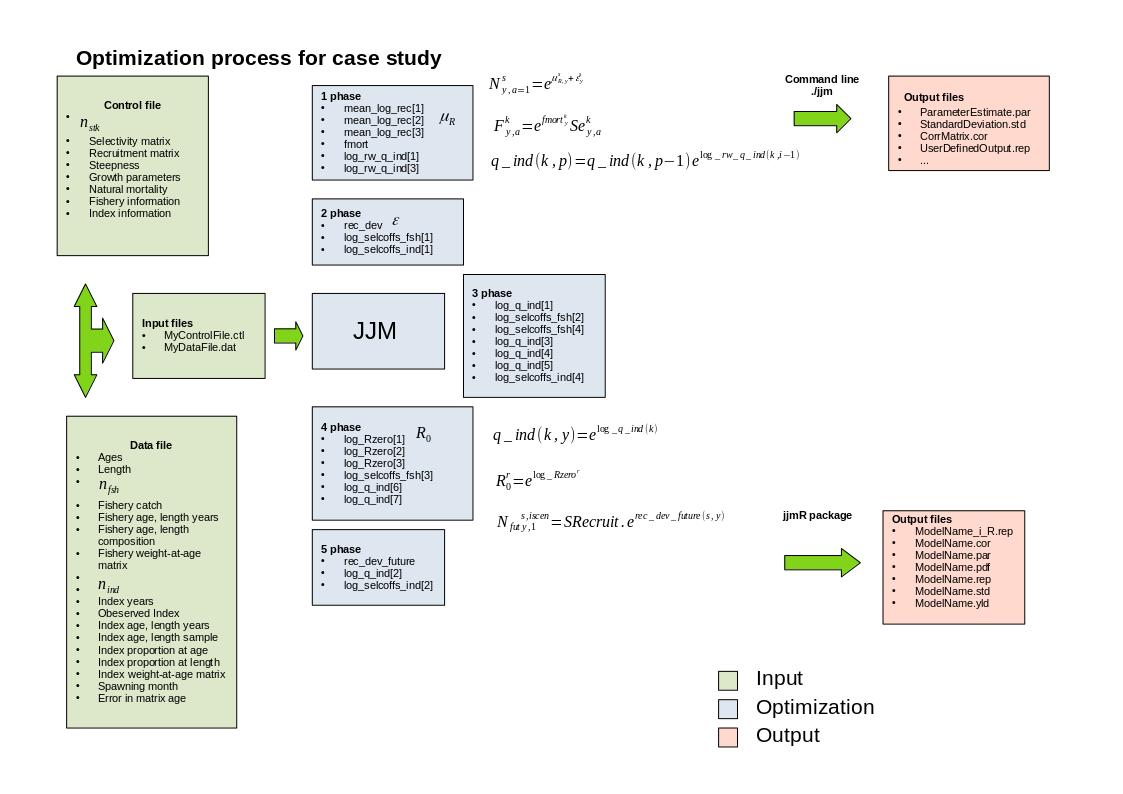
\includegraphics[scale = 0.6]{graficofases2.jpg}
    \caption{Optimization process of the JJM (Joint Jack Mackerel) model. In green: the inputs (control and data file), in each green box the respective inputs are listed. In blue: the optimization process, in this case it is a model with 5 phases; each box in blue is an optimization phase and the respective parameters to be estimated are listed. In red: the outputs, the top box represents the outputs produced when running the model using the command line, and in the bottom box the outputs using the jjmR package.}
    \label{fig:mesh1}
\end{figure}





\label{section:AppendixA}
\section{Appendix B: Assessment results of case study}
\begin{figure}[H]
    \centering
    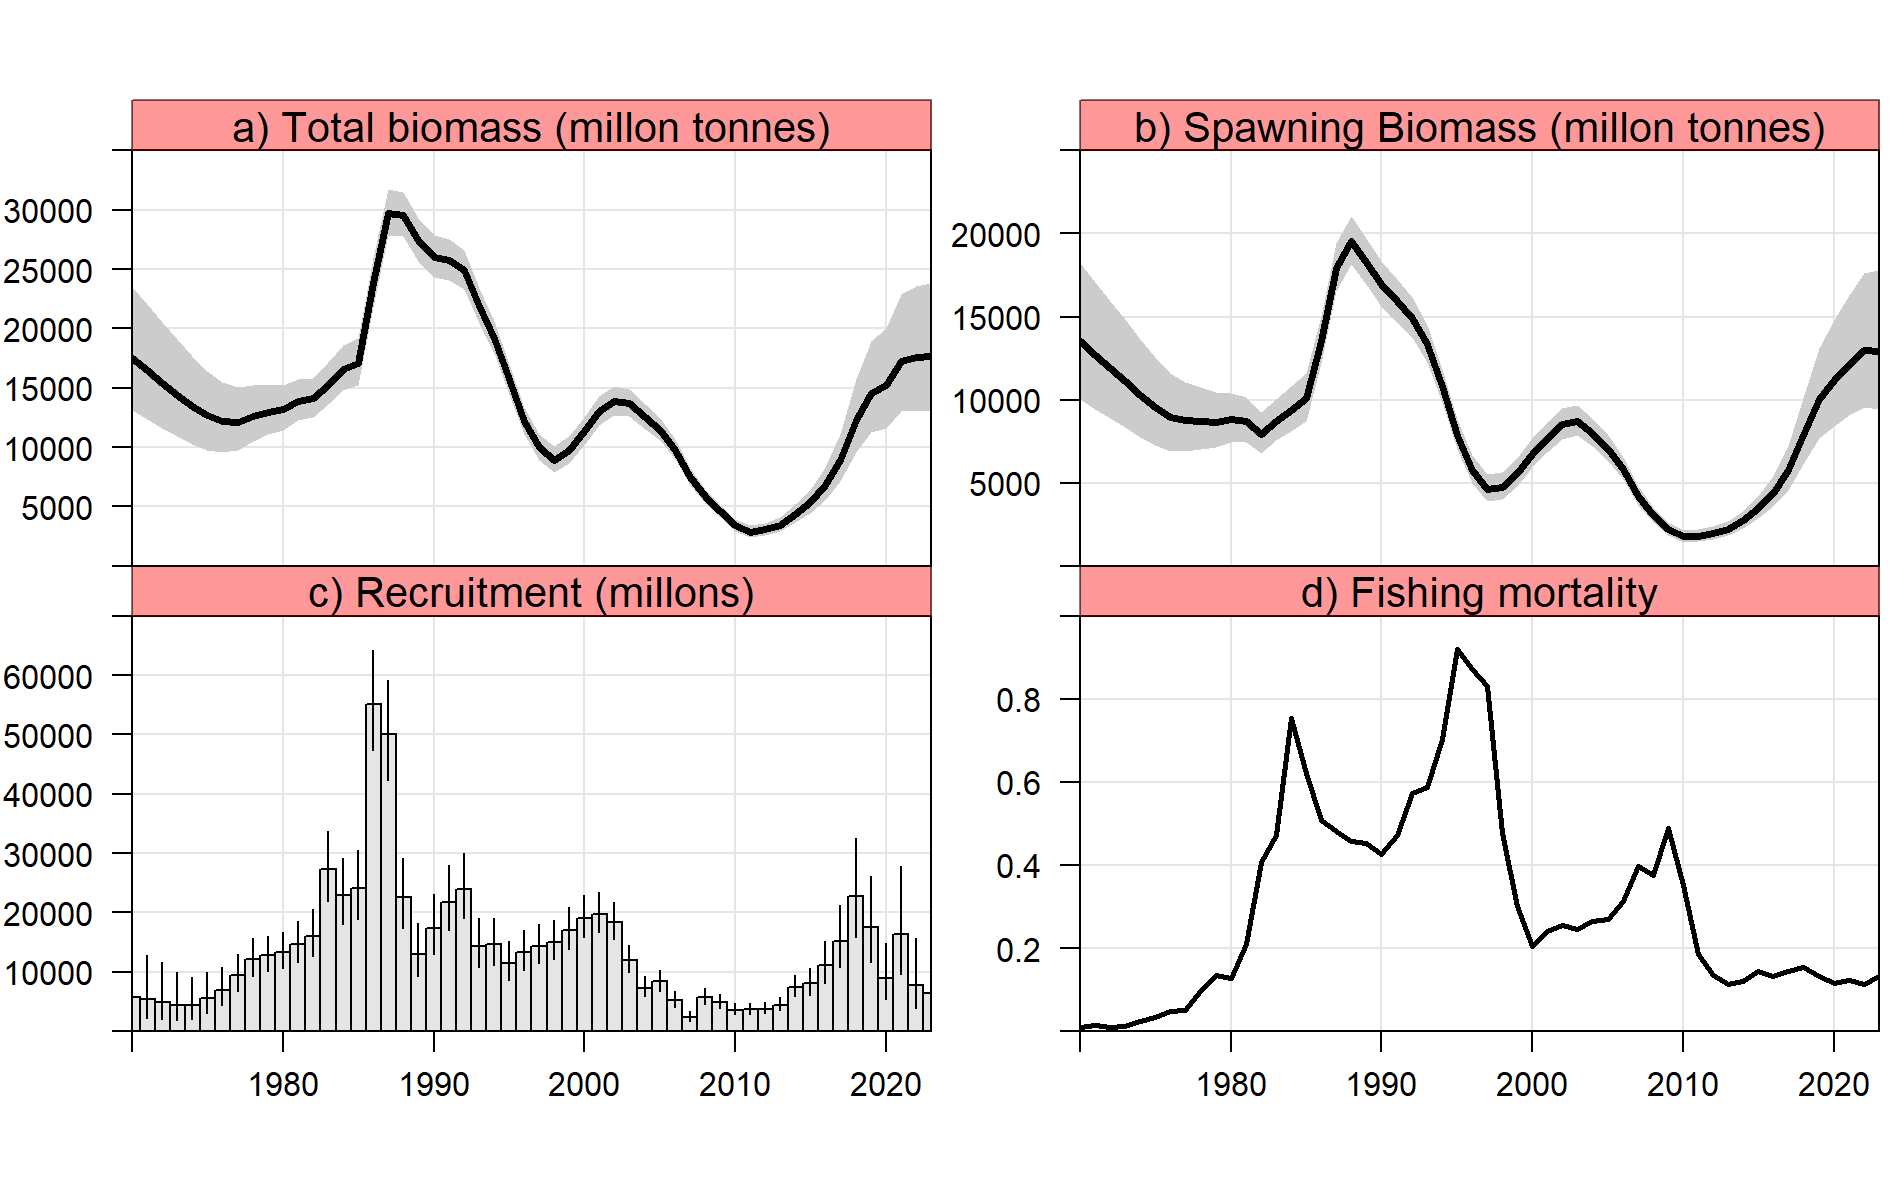
\includegraphics[scale = .9]{stock1.png}
    \caption{Plot for stock 1.  Times series of (a) Total biomass, (b) Spawning biomass, (c) Recruitment, and (d) Fishing mortality.}
    \label{fig:mesh2}
\end{figure}

\begin{figure}[H]
    \centering
    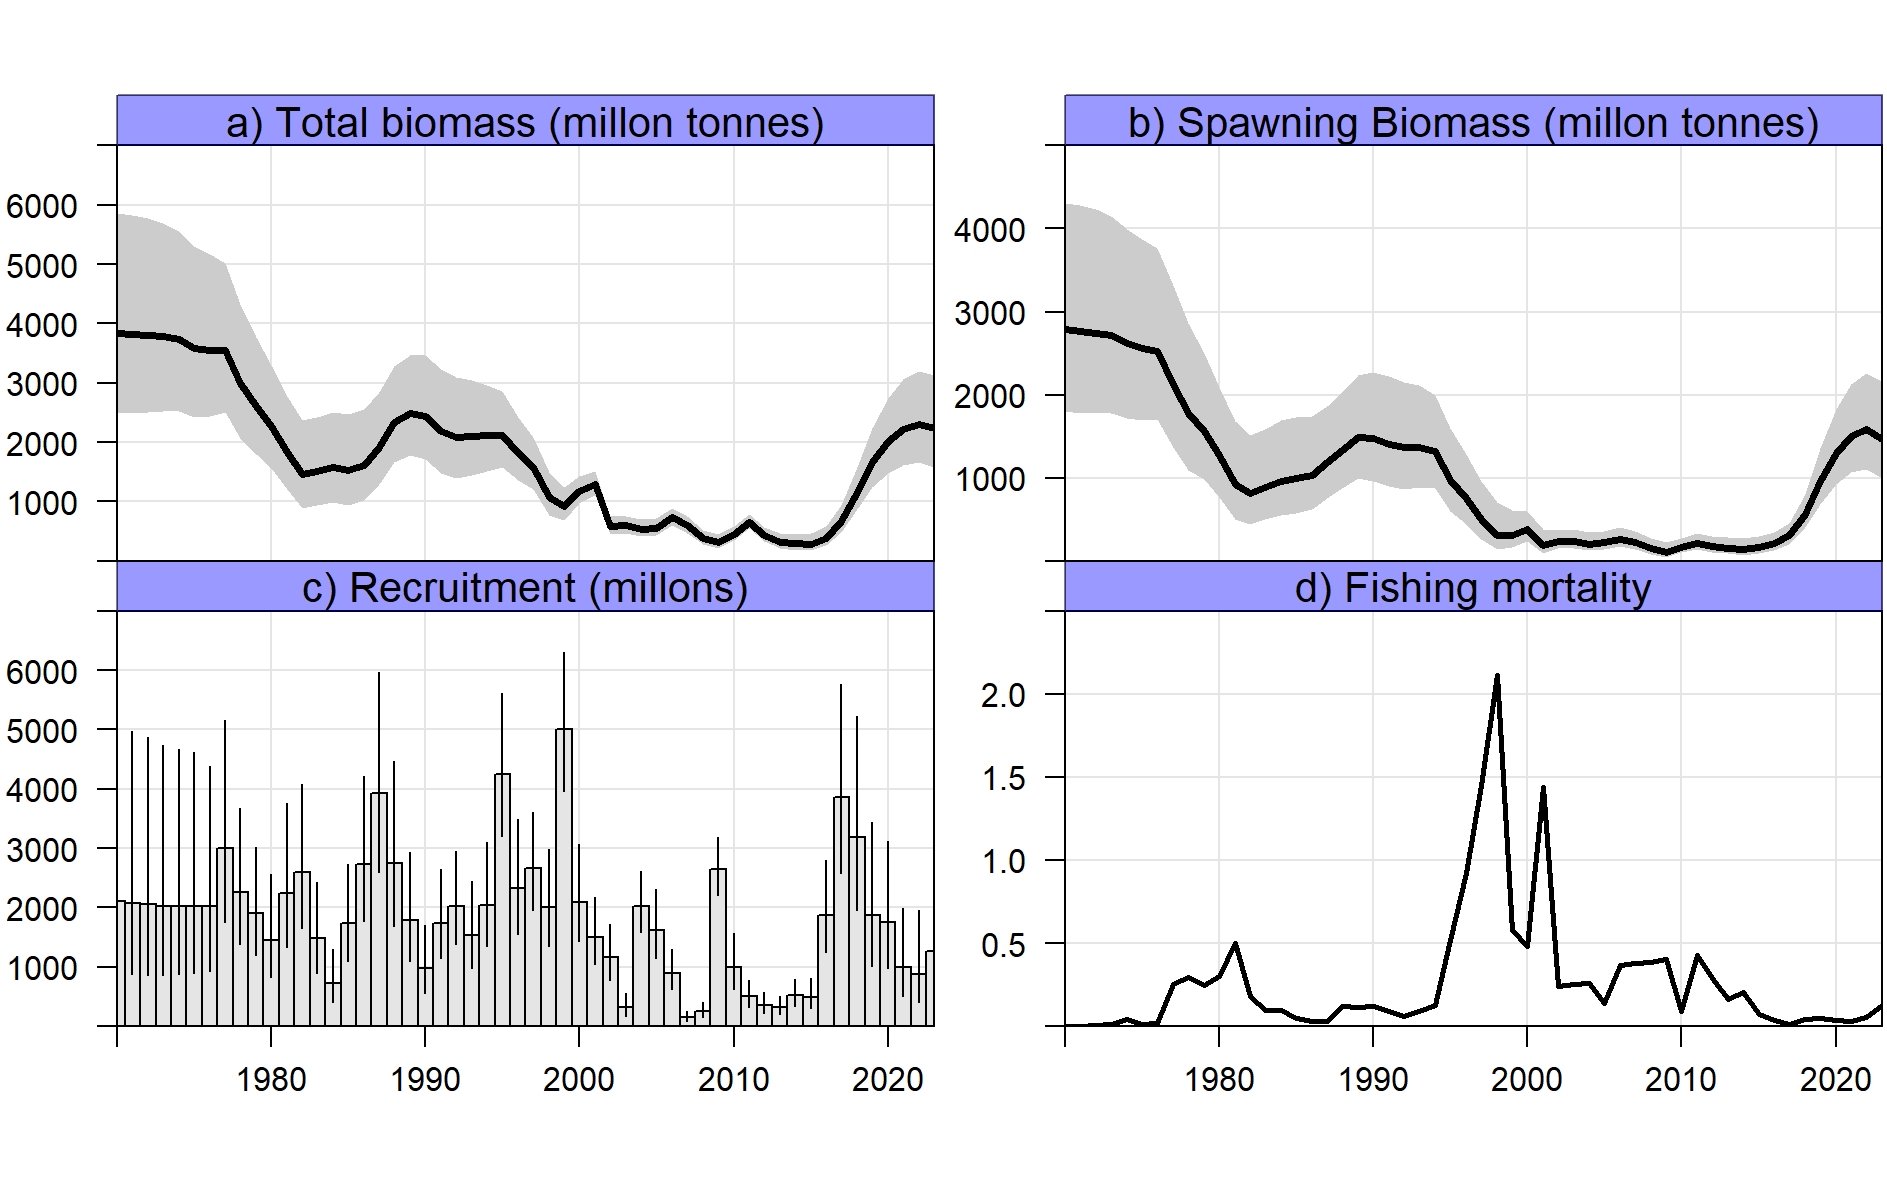
\includegraphics[scale = .9]{stock2.png}
    \caption{Plot for stock 2.  Times series of (a) Total biomass, (b) Spawning biomass, (c) Recruitment, and (d) Fishing mortality.}
    \label{fig:mesh3}
\end{figure}




\label{section:AppendixB}
%\section{Appendix: Another useful functions}
\nocite{*}



%\bibliographystyle{apelike} 
\printbibliography

% @online{
% link,
% author = "",
% url = "https://www.fisheries.noaa.gov/southeast/sustainable-fisheries/frequent-questions-annual-catch-limit-monitoring"
% }







\end{document}
